%% Hello emacs, this is -*- latex -*-
\typeout{ ====================================================================}
\typeout{ This is file main.tex, created at 23-Jan-2004 }
\typeout{ Maintained by Andre DOS ANJOS <Andre.dos.Anjos@cern.ch> }
\typeout{ ====================================================================}

\documentclass[a4paper,12pt]{report}

%% -----------------------------------------
%% Lista de Pacotes que você deverá precisar
%% -----------------------------------------
\usepackage[french,english,portuges]{babel} % Para hifenação automática.
\usepackage[T1]{fontenc} % Para a hifenação de palavras acentuadas
\usepackage[utf8]{inputenc} % Para tradução automática de acentos.
\usepackage{indentfirst}
\usepackage{tocbibind} % Para a inclusão de bibliografia e índices na ToC
\renewcommand{\tocbibname}{Referências Bibliográficas}

% André DOS ANJOS <Andre.dos.Anjos@cern.ch>
% $Id: mycolor.tex,v 1.1 2002/04/01 19:44:54 andre Exp $

% Entries that are specific to colors
%% Estes comandos aqui definem novas cores. Para usá-las, você tem que
%% incluir no seu fonte, o pacote 'color'
\usepackage{color}
\definecolor{brightred}{rgb}{1,0,0}
\definecolor{red}{rgb}{0.75,0,0}
\definecolor{darkred}{rgb}{0.5,0,0}

\definecolor{brightgreen}{rgb}{0,0.75,0}
\definecolor{green}{rgb}{0,0.5,0}
\definecolor{darkgreen}{rgb}{0,0,0.25}

\definecolor{brightblue}{rgb}{0,0,1}
\definecolor{blue}{rgb}{0,0,0.75}
\definecolor{darkblue}{rgb}{0,0,0.5}
 % Para descrever cores.
% Dear emacs, this is -*- latex -*-
% Andr� DOS ANJOS <Andre.dos.Anjos@cern.ch>
% $Id: ifpdf.tex,v 1.1 2002/04/01 19:44:54 andre Exp $

% Declares the \ifpdf command

\newif\ifpdf
\ifx\pdfoutput\undefined
    \pdffalse          % N�o estamos rodando PDFLaTeX
\else
    \pdfoutput=1       % N�s estamos rodando PDFLaTeX
    \pdftrue
\fi

 % Para a próxima seleção.
\ifpdf % Gráficos, thumbnails e hiper-referências
% André DOS ANJOS <Andre.dos.Anjos@cern.ch>
% $Id: pdfheader.tex,v 1.1 2002/04/01 19:44:54 andre Exp $

% Entries that are specific to process the document with PDFLATEX

% Ligações coloridas
%% \usepackage[pdftex,%
%% 	    colorlinks=true,%
%%             urlcolor=blue,% \href{...}{...}
%%             anchorcolor=brightblue,%
%%             filecolor=green,% \href*{...}
%%             linkcolor=red,% \ref{...} and \pageref{...}
%%             menucolor=darkblue,%
%%             citecolor=darkgreen,%
%%             pdftitle={Tese de Doutorado de André Rabello dos Anjos},%
%%             pdfauthor={Andre Rabello dos Anjos <Andre.dos.Anjos@cern.ch>},%
%%             pdfsubject={Tese},%
%%             pdfkeywords={tese doutorado andre rabello anjos},%
%%             pagebackref,%
%%             pdfpagemode=None,%
%%             bookmarksopen=true]{hyperref}

% Ligações em preto e branco para impressão
\usepackage[pdftex,%
    	    colorlinks=true,%
            urlcolor=black,% \href{...}{...}
            anchorcolor=black,%
            filecolor=black,% \href*{...}
            linkcolor=black,% \ref{...} and \pageref{...}
            menucolor=black,%
            citecolor=black,%
            pdftitle={Tese de Doutorado de Andre Rabello dos Anjos},%
            pdfauthor={Andre DOS ANJOS <Andre.dos.Anjos@cern.ch>},%
            pdfsubject={Tese},%
            pdfkeywords={tese doutorado andre rabello anjos},%
            pagebackref=false,% this enables the back reference at bibitems
            pdfpagemode=None,%
            bookmarksopen=true]{hyperref}
\pdfcompresslevel=9
\usepackage[pdftex]{graphicx}
\DeclareGraphicsExtensions{.pdf,.png,.jpg,.mps}	% modify the preferences
%%\usepackage{thumbpdf}
%%\usepackage{palatino} % try to get closer to adobe tools output


\else
% Andr� DOS ANJOS <Andre.dos.Anjos@cern.ch>
% $Id: texheader.tex,v 1.1 2002/04/01 19:44:54 andre Exp $

% Entries that are specific to process the document with simple LATEX

\usepackage{graphicx}
\usepackage[colorlinks=true,%
            urlcolor=blue,% \href{...}{...}
            anchorcolor=brightblue,
            filecolor=green,% \href*{...}
            linkcolor=red,% \ref{...} and \pageref{...}
            menucolor=darkblue,%
            citecolor=brightgreen]{hyperref}

\fi
\graphicspath{{figures/}} % Aonde encontrar as figuras...
\usepackage{rotating} % para rotacionar alguns flutuantes
\usepackage{tabularx} % para tabelas mais legais

%\usepackage[T1]{fontenc} % Para fontes mais nítidas
\usepackage[hmargin=3.0cm,vmargin=2.5cm]{geometry} % Para mais espaço no texto
%% Aumenta espaçamento para 1.5 ao invés de 1.2 para ficarmos de acordo com a
%% norma COPE
\renewcommand{\baselinestretch}{1.5}

%% --------------------------
%% Ajustando a saída HTML
%% --------------------------
%\usepackage{html} % Para usar os comandos pre-definidos por latex2html

%% --------------------------
%% Lista de Pacotes Opcionais (descomente o que for preciso)
%% --------------------------
\usepackage{amssymb} % Para os símbolos matemáticos. Coloque antes de amsmath
\usepackage{amsmath} % Para as fórmulas e ambientes.
\usepackage{multirow} % Para ter múltiplas linhas por coluna
\usepackage{hhline} % Para linhas mais interessantes em artigos
\usepackage{alltt} % Para entrada verbatim com comandos LaTeX
\usepackage{subfigure} % Para múltiplas figuras em uma só

% Algumas coisas já definidas, você deverá ter o fonte comandos.tex no
% diretório atual para poder usar estes comandos.
% $Id: comandos.tex,v 1.3 2002/04/01 19:43:59 andre Exp $

% Este fonte LaTeX deve ser inclu�do com um \input{} em outro fonte LaTeX.
% Ele consiste de novos comandos que facilitam certas atividades quando se
% est� escrevendo em LaTeX.

%% Mudan�a de linguagem com o Babel. O pacote 'babel' deve ser usado.
\newcommand{\eng}[1]{\foreignlanguage{english}{\textit{#1\/}}}
\newcommand{\fr}[1]{\foreignlanguage{french}{\em{#1\/}}}

%% Alguns atalhos
\newcommand{\eiro}{$^{\underline{o}}$} % Desenha o 'o.' do 1o.
\newcommand{\eira}{$^{\underline{a}}$} % Desenha o 'a.' de 1a.
\newcommand{\expo}[2]{$#1^{#2}\/$} % exponencia o 1o. arg com o 2o.
\newcommand{\raw}[1]{\texttt{#1}} % Vai para modo truetype (raw text)

%% Mais atalhos para �ndices remissivos e gloss�rios
\newcommand{\idx}[1]{#1\index{#1}}
\newcommand{\idxeng}[1]{\eng{#1}\index{#1}}
\newcommand{\idxfr}[1]{\fr{#1}\index{#1}}

%% Atalhos
\newcommand{\etem}{\ensuremath{\text{E}^{\text{e.m.}}_{T_{3\times7}}}}
\newcommand{\ethad}{\ensuremath{\text{E}^{\text{HAD-1}}_{T_{0,2\times0,2}}}}
\newcommand{\rcore}{\ensuremath{\text{R}^{3\times7/7\times7}_{\text{e.m.}_{2}}}}
\newcommand{\eratio}{\ensuremath{\text{R}^{\text{2-m�ximos}}_{\text{e.m.}_{1}}}}
\newcommand{\ep}{\ensuremath{\eta\times\phi}}



%% Selecione aqui o que você deseja incluir na próxima
%% impressão.

%% Parte introdutória
%\includeonly{rosto, ficha, dedicatoria, resumo, conteudo, introducao}

%% capítulo de interesse
%%\includeonly{introducao}

%% Tudo
\includeonly{rosto, ficha, dedicatoria, resumo, conteudo, introducao,%
fisica, atlas, trigger, baseline, neural, implement, conclusao2,%
coord-atlas, rna, neuralringer, published}

%\includeonly{rosto}

%% Defesa de Tema em 14 de julho de 2004
%% Defesa de Tese em 14 de dezembro de 2006
%% Entrega da versão final em 8 de janeiro de 2007

%% Hello emacs, this is -*- latex -*-
\typeout{ ====================================================================}
\typeout{ This is file title.tex, created at 29-Jun-2004 }
\typeout{ Maintained by Andre Rabello dos Anjos <Andre.dos.Anjos@cern.ch> }
\typeout{ ====================================================================}

\title{Sistema Online de Filtragem em um Ambiente com Alta Taxa de Eventos}
\author{Andr� Rabello dos Anjos (\texttt{Andre.dos.Anjos@cern.ch}) \\
	Orientador: Jos� Manoel de Seixas (\texttt{seixas@lps.ufrj.br})}

\typeout{ *************** End of file title.tex *************** }

%\includeonly{conteudo, introducao, fisica, atlas, trigger, baseline, neural,
%implement, conclusao2, coord-atlas, neuralringer, published}

%\includeonly{trigger, baseline, neural, implement, neuralringer, conclusao2}
%\includeonly{published}

%\includeonly{neural, implement}
%\includeonly{neural}

%% Preparando o índice remissivo, que é opcional
%%\usepackage{makeidx}
%%\makeindex

% O início do documento para o LaTeX2e
\begin{document}

\maketitle

% Começamos com a página de título
\begin{titlepage}
\begin{center}
{ SISTEMA ONLINE DE FILTRAGEM EM UM AMBIENTE COM ALTA TAXA DE EVENTOS }

\vspace*{1.0cm}
{André Rabello dos Anjos}
\end{center}
\vspace*{1.0cm}

{ \noindent 
TESE~~ SUBMETIDA~ AO~ CORPO DOCENTE~~ DA~ COORDENAÇÃO~ DOS
PROGRAMAS DE PÓS-GRADUAÇÃO DE ENGENHARIA DA \mbox{UNIVERSIDADE} FEDERAL~~ DO~
RIO~ DE~ JANEIRO~ COMO~ PARTE~ DOS~ REQUISITOS \mbox{NECESSÁRIOS} PARA A
OBTENÇÃO DO GRAU DE MESTRE EM CIÊNCIAS EM ENGENHARIA ELÉTRICA. }  \\

\noindent Aprovada por:
\vspace{1.0cm} % nao tinha

\begin{flushright}
\parbox{10cm}
{
\begin{center}

\rule{10cm}{.02cm} \\
Prof. José Manoel de Seixas, D.Sc. \\
\vspace{.30in}

\rule{10cm}{.02cm} \\
Prof. Sicraninho de Tal, Titulacao \\
\vspace{.30in}

\rule{10cm}{.02cm} \\
Prof. Beltraninho de Tal, Titulacao \\
\vspace{.30in}

\rule{10cm}{.02cm} \\
Prof. Nao Sei Mais O Que Inventar de Tal, Titulacao \\
\vspace{.30in}

\end{center}
}
\end{flushright}
\vspace{-.5cm}

\vfill
\begin{center}
RIO DE JANEIRO, RJ - BRASIL \\
JULHO DE 2004
\end{center}

\end{titlepage}


% A numeração aqui começa a partir de 2, em
% romano. A ficha catalográfica é obrigatória!
\pagenumbering{roman} \setcounter{page}{2}
% Esta � a ficha catalogr�fica da COPPE, como apresentado
% em suas normas de tese.

%% Define um ambiente para a ficha bibliogr�fica
\newenvironment{ficha}{%
  \newlength{\largura}% calcula a largura de 40 colunas verbatim (36...)
\settowidth{\largura}{\ttfamily aaaaaaaaaaaaaaaaaaaaaaaaaaaaaaaaaaa}%
\begin{center}%
\begin{minipage}{\largura}%
\newlength{\saveparid}% cria um reposit�rio
\setlength{\saveparid}{\parindent}% guarda o valor default
\setlength{\parindent}{0.6cm}}%
{%
\setlength{\parindent}{\saveparid}% restaura o valor default
\end{minipage}%
\end{center}}

% centraliza verticalmente
\vspace*{\fill}{
\begin{ficha}
\noindent
ANJOS, ANDR� RABELLO DOS

Sistema Online de Filtragem em um Ambiente com Alta Taxa de Eventos
[Rio de Janeiro] 2004

%% O primeiro n�mero, romanos, indica o n�mero de p�ginas at� a primeira
%% p�gina em n�mero ar�bico (equivale ao cap�tulo 1 na maior parte dos 
%% casos. O segundo n�mero equivale ao n�mero de p�ginas em ar�bico.
XVII, 167 p. 29,7 cm
(COPPE/UFRJ, D.Sc., Engenharia El�trica, 2004)

Tese - Universidade Federal do Rio de Janeiro, COPPE

\noindent
1.~F�sica de Altas Energias~ 2.~Calorimetria~ 3.~Redes Neuronais~
4.~Processamento R�pido~ 5.~Processamento Distribu�do

I.COPPE/UFRJ \hspace{.5cm} II.T�tulo (s�rie)
\end{ficha}
}
\vfill

\clearpage


% Agradecimentos e dedicatórias
%% Escreva aqui sua dedicatória e/ou agradecimentos

%% Define um ambiente para as dedicatórias e agradecimentos
\newenvironment{dedicate}[2]{%
\begin{flushright}%
\begin{minipage}{#1}%
\begin{center}
#2
\end{center}
\setlength{\saveparid}{\parindent}% guarda o valor default
\setlength{\parindent}{0.6cm}}%
{%
\setlength{\parindent}{\saveparid}% restaura o valor default
\end{minipage}%
\end{flushright}}

\vspace*{\fill}{
\begin{dedicate}{0.5\textwidth}{}
\hspace{0.8cm}Ao \textbf{grande} amor de minha vida, Aninha: você é a minha luz.
\end{dedicate}}

\clearpage
% Agradecimentos

\vspace*{\fill}{
\begin{dedicate}{0.7\textwidth}{Agradecimentos:}
\hspace{0.8cm}Em especial, a meu amor, Aninha, que suportou a minha ausência
nestes longos meses que passamos afastados por causa deste trabalho. À minha
super-mãe Léa, que nunca pára de me apoiar, te amo. Aos meus irmãos Guga e Vá,
pela amizade eterna que nutrimos uns pelos outros. Ao meu pai, por seu bom
humor de sempre e nossos almoços aos sábados. À Ira, nossa sempre-amiga e
mãe. Aos meus pais postiços, Dedé e Sidney, pela filha e pelo carinho de
sempre. A meu amigo e mestre Seixas, pelas incontáveis discussões e por me
guiar, sempre no melhor dos caminhos.
\end{dedicate}}


% Os resumos
%% Define um ambiente para o resumo, mais compacto e que dá mais texto
\newenvironment{summary}[1]{%
\begin{minipage}{\linewidth}%
\newcommand{\saveparameter}{\baselinestretch}% guarda o valor default
\renewcommand{\baselinestretch}{#1}%
\normalsize}%
{%
\renewcommand{\baselinestretch}{\saveparameter}% restaura o valor default
\end{minipage}%
}

\noindent
Resumo da Tese apresentada à COPPE/UFRJ como parte dos requisitos necessários
para a obtenção do grau de Doutor em Ciências (D.Sc.)

\vspace{1.5cm}

\begin{center}
SISTEMA ONLINE DE FILTRAGEM EM UM AMBIENTE COM ALTA TAXA DE EVENTOS
\vspace{1cm}

André Rabello dos Anjos
\vspace{1cm}

Julho/2004
\end{center}
\vspace{1.5cm}

\noindent
Orientador: José Manoel de Seixas
\vspace{1.5cm}

\noindent
Programa: Engenharia Elétrica
\vspace{2cm}

\begin{summary}{1.2}
O experimento ATLAS no CERN, Suíça, contará com um Sistema de Filtragem que
deverá separar a Física ordinária dos eventos que possam representar
decaimentos do raro bóson de Higgs. O Segundo Nível deste Sistema de
Filtragem, em específico, será constituído de cerca de 1.000 computadores
ligados em rede, processando cada um evento completo aprovado pelo Primeiro
Nível. Cada evento terá em média 10 milissegundos para ser processado.  Neste
nível, operará um conjunto de algoritmos descritos em \eng{software} que
executará a seleção de eventos. Dentre esses, algoritmos de discriminação
elétron/jato têm papel fundamental na eficiência da aquisição de dados, uma
vez que a ocorrência de elétrons pode representar a Física de interesse. Neste
trabalho apresentamos resultados obtidos para sistemas de discriminação mais
eficientes, baseados em redes neurais artificiais e um sistema de compactação
de dados que se beneficia do perfil de deposição energético de elétrons e
jatos com calorímetros para alcançar melhor eficiência de classificação. Os
resultados sugerem que a utilização de ferramentas de processamento de sinais
como a Análise de Componentes Principais e Componentes Independentes, poderá
melhorar ainda mais a qualidade da análise executada neste nível de filtragem.
\end{summary}

\clearpage

\noindent
Abstract of Thesis presented to COPPE/UFRJ as a partial fulfillment of the
\linebreak requirements for the degree of Doctor of Science (D.Sc.)

\vspace{1.5cm}

\begin{center}
ONLINE TRIGGER SYSTEM FOR A HIGH EVENT RATE ENVIRONMENT 
\vspace{1cm}

André Rabello dos Anjos
\vspace{1cm}

July/2004
\end{center}
\vspace{2cm}

\noindent
Advisor: José Manoel de Seixas
\vspace{2cm}

\noindent
Department: Electrical Enginnering
\vspace{2cm}

\begin{summary}{1.2}
(esta tradução já não condiz com o texto original em português...)
The ATLAS experiment at CERN, Switzerland, will count on a Trigger System that
separates the ordinary Physics from that which represents decays of the rare
Higgs boson. This system was initially designed to operate in 3 levels
cascade-conneted, with higher complexity, detection quality and operation time
per event. The Second Level Trigger, specifically, will be made out of 1,000
commodity computers interconnected forming a network, processing each a full
single event approved by the First Level. Each event shall have an averaged
processing time of 10 miliseconds.

At the second level of this system, operates a set of algorithms described in
software, that will execute the event selection. Among those, electron/jet
discriminators play a fundamental role for the overall efficiency, since
electrons may represent interesting Physics. This work presents results
obtained for more efficient discriminating systems, based on artificial neural
networks. The results suggest that the use of signal processing tools like
Principal Component Analysis or Independent Components may improve even more
the analysis quality executed at this trigger level.
\end{summary}


% Aqui você poderá anexar a lista de
% conteúdos, lista de figuras e tabelas
% do documento. 
\tableofcontents
\clearpage
\listoffigures
\clearpage
\listoftables
\clearpage
\printglossary
\clearpage



% Normalmente, eu uso o arquivo principal somente para os detalhes de
% apresentação, deixando o conteúdo em arquivos isolados. Se você quiser
% fazer o mesmo, descomente as linhas abaixo e troque o nome dos arquivos
% contendo as seções ou capítulos. Lembre-se, o processador LaTeX vai
% procurar seus arquivos em arquivo.tex se você fizer \input{arquivo}

\pagenumbering{arabic}
\chapter{Introdu��o}
\label{chap:introducao}

\idx{F�sica de Part�culas} ou \idx{F�sica de Altas Energias} (do ingl�s,
\idxeng{High Energy Physics}, comumente abreviado por \eng{HEP}) denominam o
ramo da f�sica que estuda a mat�ria enquanto formada por part�culas
subat�micas como el�trons, quarks e pr�tons, e suas propriedades. Neste
cap�tulo, introduzimos seus conceitos fundamentais, iniciando com um breve
hist�rico desta �rea.

%% Advocate: necess�rio para o leitor entender porqu� fala-se que o CERN �
%% o topo de gama neste campo!

\section{Um pouco de hist�ria}

Desde a antiguidade, as pessoas t�m buscado entender o comportamento da
mat�ria: \textit{- Porque objetos largados caem no ch�o?}, \textit{- Porque
  materiais diferentes tem propriedades diferentes}, e assim por
diante. Outros mist�rios incluem a caracter�stica do pr�prio universo onde
habitamos e o comportamento dos corpos celestes. Muitas teorias foram
propostas desde ent�o, a maior parte errada, embora este seja um efeito
colateral da empreitada cient�fica. As teor�as f�sicas na antiguidade eram
baseadas somente em termos filos�ficos e raramente verificadas por testes
experimentais sistem�ticos \cite{partadv}.

No in�cio do s�culo XVII, Kepler formulou um modelo do sistema solar baseado
em cinco s�lidos plat�nicos, em uma tentativa de explicar porque as orbitas
dos planetas tinha os tamanhos relativos observados. Seu acesso a observa��es
acuradas realizadas por outro cientista da �poca o capacitou a determinar que
seu modelo estava inconsistente com as �rbitas observadas. Depois de um
esfor�o her�ico de 7 anos, Kepler concluiu que os planetas n�o descrevem uma
�rbita circular, mas el�pticas, tendo o Sol em um de seus focos. Kepler tamb�m
sugeriu que uma "for�a" emanado do Sol afastaria os planetas de suas �rbitas
naturais, levando-os a perseguir uma �rbita el�ptica.

Durante este mesmo s�culo, Galileu fez-se do uso, pela primeira vez, de um
"experimento" no sentido acad�mico da palavra, para validar teorias f�sicas,
o que � uma id�ia-chave no m�todo cient�fico atual. O uso do experimento por
Galileu e sua insist�ncia de que os resultados observados ter�o sempre que
anteceder os resultados te�ricos, limparam a aceita��o de "dogmas" e fizeram
nascer uma nova era onde as id�ias cient�ficas eram abertamente discutidas e
rigorosamente testadas.

Dentre outros grandes momentos, em 1687, \idx{Isaac Newton} publicou o
\eng{Principia Mathematica}, detalhando dois compreensivos e bem sucedidos
modelos f�sicos: a lei do movimento, de onde parte a mec�nica cl�ssica; e a
lei da gravidade, que descreve esta for�a fundamental. Ambas as teorias
concordavam bastante bem com experimentos executados na �poca. A mec�nica
cl�ssica foi exaustivamente extendida por v�rios outros cientistas que
produziram novas formula��es, princ�pios e resultados.

O in�cio do s�culo XX iniciou uma revolu��o na f�sica. As aclamadas teorias
newtonianas mostraram-se incorretas em v�rias circunst�ncias. N�o somente a
\idx{Mec�nica Qu�ntica} mostrou que as leis do movimento n�o se confirmavam em
pequenas escalas, como ainda mais inquietante, a relatividade geral mostrou
que o fundo fixo do espa�o-tempo, no qual a mec�nica newtoniana e a
relatividade especial dependiam, n�o poderia existir.

Em 1904, Thomson prop�s o primeiro mod�lo at�mico, conhecido como
\idx{"Pudim de Ameixas"}\footnote{A exist�ncia do �tomo tinha sido proposta
em 1808 por Dalton.}. J� em 1905, apenas um ano depois, Einstein formulou a
"Teoria de Relatividade Especial", unificando espa�o e tempo em uma entidade
singular, chamada de espa�o-tempo. Em 1915, o pr�prio extendeu sua teoria de
relatividade especial com a "Teoria de Relativade Geral", substituindo a lei
newtoniana sobre a gravidade. As teorias de Newton e Einstein concordam para
regimes de pouca massa e energia.

Ainda em 1911, Rutherford deduziu a exist�ncia de um \idx{n�cleo at�mico}
compacto, consistindo de cargas positivas chamadas de \idx{pr�tons}. Para tal,
utilizou-se de um feixe de part�culas alfa, emitido por uma fonte radioativa,
uma folha de ouro e um simples detetor feito de Sulfeto de Zinco para testar
sua teoria \cite{halliday}. As part�culas alfa, ao baterem no detetor,
marcavam-no (veja a configura��o do experimento de Rutherford na
Figura~\ref{fig:rutherford}). Embora n�o pudesse ver o que ocorria no mundo
sub-at�mico, Rutherford podia teorizar, testar sua hip�tese e ent�o analisar
os dados experimentais para verificar se seus c�lculos estavam corretos. A
�nica teoria cab�vel, ap�s seus experimentos, � que o �tomo teria que ser
composto por um n�cleo compacto e positivo e uma periferia negativamente
carregada, de part�culas mais leves e menores que aquelas no n�cleo.

\begin{figure}
\begin{center}
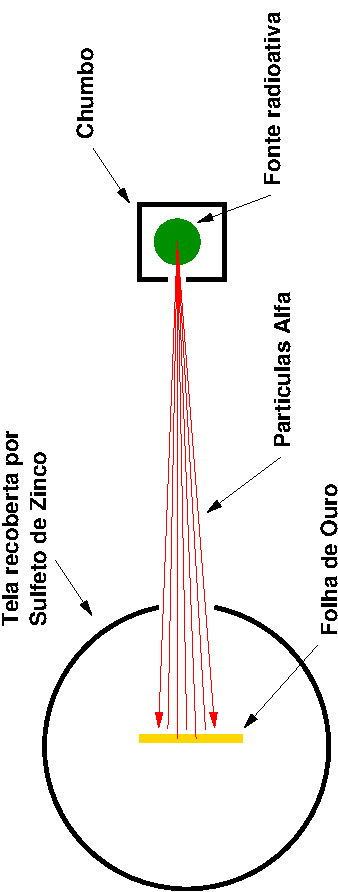
\includegraphics[scale=0.9,angle=-90]{rutherford}
\end{center}
\caption[O \eng{setup} de Rutherford.]{A configura��o do experimento de
Rutherford para a constata��o de que o n�cleo at�mico era denso e positivo.}
\label{fig:rutherford}
\end{figure}

Os \idx{Neutrons}, os constituintes nucleares de carga neutra, foram
descobertos em 1932 por Chadwick. Planck e Bohr entre outros f�sicos
desenvolveram as teorias qu�nticas para explicar v�rias anomalias
experimentais introduzindo o conceito de n�veis (ou \idxeng{quanta}) de
energia. Em 1925, Heisenberg e Schr�dinger formularam a \idx{Mec�nica
Qu�ntica}, que explica as teoricas qu�nticas anteriores. Nesta �rea, os
resultados de medidas f�sicas s�o de natureza inerentemente probabil�stica. A
teoria modela o c�lculo destas probabilidades e, de forma bem-sucedida,
descreve o comportamento da mat�ria em pequenas escalas.

A mec�nica qu�ntica tam\-b�m fornece ferramentas te\-�\-ri\-cas para a
f�\-si\-ca de ma\-t�\-ria condensada, que estuda o comportamento f�sico de
s�lidos e l�quidos, incluindo fen�menos de cristaliza��o, semi-condutividade e
super-condutividade.

A \idx{Teoria Qu�ntica dos Campos} foi formulada para estender a mecanica
qu�ntica fazendo-a consistente com a relatividade especial, atingindo sua
forma moderna no final dos anos 40 com o trabalho de Feynman, Schwinger,
Tomonaga e Dyson. Eles formularam a \idx{Eletrodin�mica Qu�ntica}, que
descreve a intera�ao eletromagn�tica.

A teoria qu�ntica dos campos fornece o ferramental de fundo para a f�\-si\-ca de
par\-t�\-cu\-las moderna, que estuda primordialmente as for�as elementares entre as
part�culas. Em 1954, Yang e Mills desenvolveram uma classe de teorias de
Gauge, introduzindo o \idx{Modelo At�mico Padr�o} ou simplesmente \idx{Modelo
Padr�o}, que foi completado nos anos 70. O Modelo Padr�o descreve de forma
bem-sucedida quase todas as part�culas elementares observadas at� hoje e
encompassa as \idx{for�as fundamentais} "forte", "fraca" e "eletromagn�tica"
assim como as part�culas de que se comp�e toda a mat�ria. O Modelo Padr�o n�o,
no entanto, uma teoria fundamental de todas a intera��es existentes na
natureza, primariamente por n�o descrever a gravidade.

\section{F�sica de part�culas moderna}

Embora de grande sucesso modelando resultados encontrados
ex\-pe\-ri\-men\-tal\-men\-te, o Modelo Pa\-dr�o nunca foi aceito como uma
teoria completa de f�sica fundamental. Isto acontece por causa de dois
aspectos:

\begin{enumerate}
\item O modelo cont�m 19 par�metros livres, como a massa das part�culas, que
  precisam ser determinados experimentalmente (e mais outros 10 para massas de
  neutrinos). Estes par�metros n�o podem ser calculados independentemente;

\item O modelo n�o descreve a intera��o gravitacional;
\end{enumerate}

Desde a comple��o do Modelo Padr�o, muitos esfor�os foram travados para
resolver ambos os pontos. Um deles � conhecido como a \idx{Grande Unifica��o},
do qual muitos aspectos est�o bastante longe de serem observados em
laborat�rio. O \idx{b�son de Higgs}, que � previsto pelo modelo padr�o ainda
n�o foi observado at� os dias de hoje. Alguns experimentos, dentre os quais o
experimento \idx{ATLAS} (do ingl�s, \eng{A Toroidal LHC Apparatus}) no
\idx{CERN}, Su��a, est� sendo constru�do para o estudo desta f�sica.

\subsection{Aceleradores e Detetores}

De forma parecida a Rutherford, os f�sicos atuais usam um feixe de part�culas
aceleradas para criar em laborat�rio condi��es que permitam o estudo da
intera��es sub-at�micas que se deseja estudar. Este feixes podem colidir com
um alvo fixo ou com um outro feixe de part�culas, que � acelerado em dire��o
contr�ria ao feixe prim�rio. Para visualizar eletronicamente os sub-produtos
de tais intera��es f�sicas, utilizam-se m�ltiplos detetores.

A acelera��o das part�culas resolve dois problemas que os f�sicos de hoje
encontram em seus experimentos:

\begin{enumerate}
\item Comprimento de Onda - O comprimento de onda determina a acur�cia do que
� poss�vel observar \cite{partadv}.

Uma vez que par\-t�\-culas tam\-b�m apresentam caracte\-r�s\-ticas de onda, n�o
� pos\-s�\-vel obter uma medida acurada usando-se part�culas comuns, como um
e\-l�\-tron, na observa��o de part�culas muito pequenas. Um el�tron n�o serve,
nem mesmo, para observar outro el�tron. A acelera��o da part�cula, no entanto,
aumenta seu momento, diminuindo\footnote{O comprimento de onda e o momento de
um corpo s�o inversamente proporcionais.} seu comprimento de onda e permitindo
que medidas acuradas possam ser tomadas usando-se part�culas maiores, como
el�trons.

\item Energia Cin�tica - Deseja-se, nos experimentos modernos, que o impacto
seja o mais aniquilador poss�vel. Isto � interessante, pois ao se aniquilar
mat�ria, liberando muita energia, part�culas mais massivas e menos est�veis s�o
geradas. Ao se acelerar uma part�cula, aumenta-se sua energia cin�tica,
tornando a colis�o com o alvo mais eficiente (melhor aniquila��o).
\end{enumerate}

\subsection{A acelera��o das part�culas}

A acelera��o de part�culas \index{acelera��o de part�culas} � um processo
bastante simples: inicialmente deve-se escolher part�culas eletricamente
carregadas para um experimento - e\-l�\-trons, p�\-sitrons, pr�\-tons,
anti-\-pr�\-tons ou �ons, num geral, s�o aconse\-lh�\-veis. As par\-t�\-culas
eletricamente carregadas s�o posicionadas no interior de um t�nel e excitadas a
acelerar por pulsos eletromagn�ticos \index{pulsos eletromagn�ticos}. A
Figura~\ref{fig:acelera} exemplifica como el�trons s�o acelerados por pulsos
eletromagn�ticos (e.m.): as ondas e.m. aceleram as part�culas, pois elementos
eletricamente carregados adquirem for�a (acelera��o) quando envoltos
por um campo eletromagn�tico.

\begin{figure}
\begin{center}
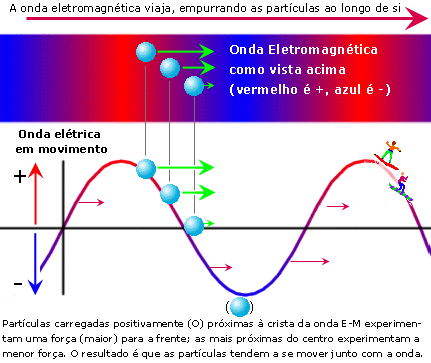
\includegraphics[scale=0.7]{static-wave}
\end{center}
\caption[A acelera��o de part�culas.]{A acelera��o de part�culas eletricamente
carregadas usando-se de pulsos e.m..}
\label{fig:acelera}
\end{figure}

Os aceleradores podem ter dois formatos\index{acelerador!tipos}: linear e
circular. Num acelerador linear\index{acelerador!linear}, as part�culas s�o
injetadas em uma extremidade e percorrem uma reta at� que colidam com outras
part�culas ou com um alvo fixo. A outra possibilidade � ter um acelerador
circular ou
s�ncrotron\index{acelerador!circular}\index{acelerador!s�ncrotron|see{acelerador
circular}}. Num acelerador circular, as part�culas s�o injetadas em um ponto do
anel de acelera��o e l� permanecem at� que tenham adquirido velocidade
suficiente ao experimento a que se destinam. A acelera��o circular exige que
magnetos poderosos curvem a trajet�ria das part�culas injetadas. Aceleradores
circulares tamb�m permitem que v�rios experimentos sejam conduzidos em pontos
de sua circunfer�ncia, simultaneamente. Aceleradores circulares possuem uma
desvantagem: quanto maior a energia necess�ria no centro de impacto, maior deve
ser o per�metro de sua circunfer�ncia.

\subsection{Dete��o: vendo o que ocorreu a\-p�s a coli\-s�o}

Depois de um acelerador ter ``bombeado"\ energia suficiente para suas
par\-t�\-culas, elas colidem com um alvo fixo ou, ent�o, com as part�culas de
outro feixe acelerado. Cada uma dessas colis�es forma um \emph{evento}
f�sico. O objetivo dos f�sicos � isolar cada evento, coletar dados a seu
respeito e verificar se o processo do qual a part�cula participou est� de
acordo com a teoria que est� sendo testada no experimento em quest�o.

A an�lise de cada evento � muito complexa, porque muitas part�culas s�o
produzidas. A maioria dessas part�culas (ou ``objetos") t�m tempo de vida t�o
diminuto que viajam por dist�ncias extremamente curtas, antes de deca�rem em
outras part�culas, sem deixar pistas aparentemente detet�veis.

Para procurar esses v�rios objetos e os produtos de seu decaimento, os f�sicos
projetam detetores com multi-componentes, que testam diferentes aspectos de um
evento. Cada componente de um detetor moderno � usado para medir v�rios
par�metros das part�culas provenientes de um evento, e/ou distinguir os
diferentes tipos de objetos gerados.  Quando todos esses componentes funcionam
juntos para detetar um evento, part�culas individuais podem ser distinguidas da
multid�o para efeito de an�lise.

Seguindo cada evento, os sistemas de processamento coletam e interpretam a
vasta quantidade de dados dos detetores e apresentam os resultados extrapolados
aos f�sicos.

Os f�sicos interessam-se pelos eventos que ocorrem durante ou mesmo depois da
colis�o das part�culas. Por essa raz�o, colocam detetores em regi�es nas quais
os objetos resultantes daquela intera��o passar�o. Os detetores s�o constru�dos
de diferentes maneiras, dependendo do tipo de colis�o analisada:

\begin{description}
\item[Alvo fixo] Num experimento envolvendo um alvo fixo, as part�culas
produzidas geralmente projetam-se para frente; por isso, os detetores s�o na
forma de cones e s�o colocados ao longo da dire��o do feixe;

\item[Feixes de colis�o] Durante um experimento envolvendo feixes em
co\-li\-s�o, as par\-t�\-cu\-las s�o espalhadas em todas as dire��es; assim, o
detetor mais adequado � esf�rico ou, mais comumente, cil�ndrico.
\end{description}

\subsubsection{Composi��o dos detetores}

Os detetores modernos s�o feitos de pe�as distintas, que testam diferentes
aspectos de um evento. Esses v�rios componentes s�o organizados de tal maneira
que os f�sicos possam obter o m�ximo de informa��o sobre as part�culas geradas
durante um evento. A Figura~\ref{fig:modern-detect} mostra um diagrama
esquem�tico de um detetor cil�ndrico moderno. Uma figura humana � mostrada em
escala, indicando a enormidade dos detetores t�picos de altas energias.

\begin{figure}
\begin{center}
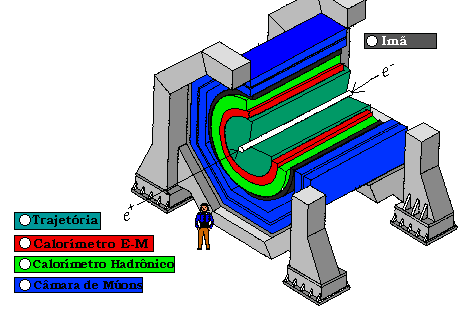
\includegraphics[scale=0.7]{modern_detect}
\end{center}
\caption{O diagrama de um detetor cil�ndrico moderno.}
\label{fig:modern-detect}
\end{figure}

Na Figura~\ref{fig:modern-detect}, � poss�vel observar que um detetor moderno
� composto de 4 sub-detetores principais. O primeiro detetor, de dentro para
fora (tomando o feixe de part�culas como origem), tem a fun��o de determinar a
rota e curvatura de part�culas, por isto � chamado de detetor de trajet�ria ou
tra�os. A curvatura das part�culas sobre o campo magn�tico a que s�o expostas
no detetor d� informa��es sobre a carga da part�cula e seu momento. O segundo
detetor � chamado calor�metro eletromagn�tico (e.m.) e tem a fun��o de
determinar a energia total de el�trons, p�sitrons e f�tons (raios
$\gamma$). Estas part�culas decaem, formando chuveiros de outros el�trons,
p�sitrons e f�tons por dentro do calor�metro e.m.. O terceiro detetor, o
calor�metro hadr�nico, mede a energia total de chuveiros originados por
h�drons (pr�tons, n�utrons ou m�sons). � composto de material pesado, que
for�a o decaimento dos h�drons num chuveiro hadr�nico, bem mais largo e
profundo que o eletromagn�tico. O quarto detetor � um detetor de
m�ons. Somente estas part�culas e neutrinos escapam dos outros sistemas de
dete��o. Neutrinos, infelizmente, nem por este �ltimo s�o detetados. Sua massa
pode ser calculada, no entanto, atrav�s da energia faltante no evento. A
Figura~\ref{fig:decay} mostra como alguns tipos de part�culas interagem com
estes detetores. F�tons, por exemplo, t�m carga nula e n�o s�o detetados pelos
detetores de tra�os, mas interagem com os calor�metros e.m.. El�trons e
p�sitrons interagem tanto com os detetores de tra�os quanto com o calor�metro
e.m., desenvolvendo cascata e.m. neste �ltimo. Pr�tons s�o detet�veis pelos
detetores de tra�os, mas desenvolvem cascata somente nos calor�metros
hadr�nicos. N�utrons somente desenvolvem cascata nos detetores hadr�nicos.

\begin{figure}
\begin{center}
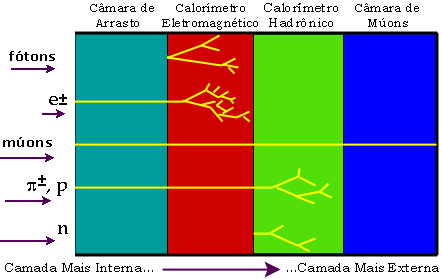
\includegraphics[scale=0.6]{decay_chart}
\end{center}
\caption{A intera��o de part�culas com os detetores modernos.}
\label{fig:decay}
\end{figure}

\section{Calorimetria moderna}
\index{Calorimetria}

Em espec�fico, \idx{Calor�metros} s�o detetores compostos utilizando a
absor��o total de part�culas para medir a energia e a posi��o de part�culas e
jatos. Durante o processo de absor��o, chuveiros s�o gerados por cascatas de
intera��es, e da� o nome ocasionalmente utilizando "contador de
chuveiros". Durante a forma��o do chuveiro, eventualmente, a maior parte da
part�cula ser� convertida em radia��o ou "calor", que explica o nome deste
tipo de detetor. � claro, nenhuma temperatura � medida, mas as caracter�sticas
de intera��o com a mat�ria (e.g. excita��o at�mica, ioniza��o) s�o utilizadas
para gerar um efeito detet�vel, atrave de part�culas carregadas. A
calorimetria � tamb�m a �nica forma previs�vel de medir part�culas neutras
entre as secund�rias produzidas em uma colis�o de altas energias
\cite{bock:detector, booth}.

Estes detetores s�o normalmente compostos de diferentes partes e t�m seu
desempenho otimizado para as diferentes part�culas que indir�o sobre seu
corpo. Cada calor�metro � feito de m�ltiplas \idx{c�lulas} individuais, sobre
o qual o volume a energia absorvida � integrada. As c�lulas s�o alinhadas para
formar torres tipicamente na dire��o de incid�ncia. A an�lise da energia
depositada nas c�lulas e torres permite medir o perfil lateral e longitudinal
das cascatas e da� sua geometria ser otimizada para este prop�sito.

Tipicamente \idx{part�culas eletromagn�ticas} incidentes (i.e. el�trons e
f�tons), s�o completamente absorvidos em calor�metros eletromagn�ticos, a
primeira das camadas de calor�metros compostos. Sua constru��o aproveita-se da
geometria de chuveiros eletromagn�ticos que s�o compactos e curtos para medir
a energia e posi��o com precis�o �tima para estas part�culas, que incluem
$\pi^{0}$'s, decaindo eletromagneticamente.

\idx{H�drons} incidentes (pr�tons, neutrons, etc.), diferentemente,
\textbf{podem} come�ar seu decaimento no calor�metro eletromagn�tico, mas
quase sempre somente ser�o completamente absorvidos em camadas posteriores,
i.e. em \idx{calor�metros hadr�nicos}, constru�dos exatamente para conter
estes chuveiros. Chuveiros hadr�nicos t�m formato bastante diversificado.

A discrimina��o, comumente no sistema de filtragem do experimento, entre
chuveiros eletromagn�ticos e hadr�nicos � um crit�rio importante para um
calor�metro. Portanto, � importante conter chuveiros eletromagn�ticos em um
espa�o mais curto, sem que se inicie um grande n�mero de chuveiros hadr�nicos.

Calor�metros tamb�m prov�m assinaturas para part�culas que n�o s�o absorvidas:
\idx{m�ons} e \idx{neutrinos}. M�ons n�o formam chuveiro na mat�ria, mas sua
carga deixa um signal de ioniza��o, que pode ser identificado em um
calor�metro se a part�cula est� suficientemente isolada (e a eletr�nica
associada permitir), e ent�o pode ser associada a um tra�o detetado nos
detetores de tra�o ou no detetor de m�ons. Neutrinos, por outro lada, n�o
deixam sinais em um calor�metro, mas sua exist�ncia pode ser algumas vezes
inferida atrav�s do princ�pio da conserva��o de energia: num calor�metro
hermeticamente fechado, ao menos um neutrino suficientemente energ�tico ou
grupo desbalanceado de neutrinos pode ser observado formando-se a soma
vetorial de todos os outros momentos medidos, tomando a energia observada em
cada c�lula do calor�metro. A precis�o de tais m�todos, usualmente limitada a
dire��o transversal, requer um vazamento m�nimo de energia em todas as
dire��es e da� o desafio para o projeto de calor�metros na pr�tica.

O desenvolvimento do chuveiro � um \idx{processo estat�stico}. Isto explica
porque a acur�cia das medidas de energia em calor�metros aumenta com o aumento
da energia de part�culas indentes, de acordo com a f�rmula emp�rica:

\begin{equation}
  \frac{\sigma_{E}}{E} \approx \frac{a}{\sqrt{E}} \beta
\end{equation}

Onde $E$ � a energia da part�cula incidente e $\sigma_{E}$ representa o desvio
padr�o da medida de energia e $a$ e $\beta$ s�o constantes que dependem do
tipo de detetor, e.g. sua espessura e caracter�sticas das camadas ativas e
passivas.

Quanto � constru��o, � poss�vel distinguir-se os seguintes tipos de calor�metro:

\begin{itemize}
  \item \textbf{Homog�neos:}\index{Calor�metro!Homog�neo} Em calor�metros
  deste tipo as fun��es de absor��o e gera��o e leitura de sinais s�o
  combinadas em um �nico tipo de material. Estes materiais s�o quase que
  exclusivamente usados para calor�metros eletromagn�ticos, por exemplo
  cristais, materiais compostos ou gases nobres em estado l�quido;

  \item \textbf{Heterog�neos:}\index{Calor�metro!Heterog�neo} Tamb�m conhecidos
  como \idx{ca\-lo\-r�\-me\-tros de a\-mos\-tra\-gem}. Neste tipo de detetor as fun��es de
  absor��o de energia e leitura do sinal s�o separadas. Isto permite uma
  escolha �tima do material de absor��o e liberdade no tratamento do
  sinal. Calor�metros heterog�neos s�o, em sua maior parte, constru�dos como
  sandu�ches (e.g. a�o, ferro e ur�nio), alternando estes materias com camadas
  de material ativo (e.g. cintiladores l�quidos ou s�lidos ou contadores
  proporcionais). Somente parte da energia do chuveiro absorvida pelo material
  ativo � medida. Calor�metros hadr�nicos, necessitando de uma profundidade
  consider�vel e largura para criar e absorver os chuveiros, s�o
  necessariamente deste tipo.

  Em constru��es modernas, a propor��o entre a energia perdida no material
  passivo ou nos absovedores � bastante grande, tipicamente na ordem de
  10. Ainda que o desempenho n�o dependa fortemente da orienta��o, a espessura
  n�o pode variar em demasiado para assegurar uma resolu��o independente da
  dire��o e da posi��o dos chuveiros.
\end{itemize}

A calorimetria moderna � a arte de escolher entre duas restri��es
conflitantes; a principal � normalmente formulada em termos da resolu��o em
energia, coodernadas espaciais, capacidade de filtragem, dureza � radia��o dos
materiais usados e em par�metros eletr�nicos como a faixa de opera��o e a
extra��o de sinais. Na maior parte dos casos, o custo final de produ��o � o
par�metro mais limitante. O n�mero de solu��es em calorimetria � maior para
calor�metros que detetores de tra�os, e solu��es bastante engenhosas foram
encontradas nos �ltimos 15 anos \cite{hadcal}.

Dentre as raz�es pelas quais os calor�metros emergiram como detetores-chave em
praticamente todos os experimentos em f�sica de part�culas est�o
\index{Calor�metro!vantagens}:

\begin{enumerate}
\item Calor�metros s�o sens�veis a part�culas neutras e carregadas;
\item Devido a diferen�as na forma de deposi��o de energia das part�culas, a
identifica��o de part�culas com alta efici�ncia pode ser atingida usando-se
calor�metros;
\item Quanto maior a energia da part�cula, mais acurado � o resultado. Isto n�o
acontece com outros tipos de detetores;
\item Para conter o desenvolvimento de cascatas dos objetos a serem medidos, a
profundidade dos calor�metros aumenta logaritmicamente com a energia, o que
permite o projeto de detetores mais compactos;
\item N�o precisam de campos magn�ticos (como os detetores de tra�os);
\item Podem ser segmentados, o que permite acurada medida da energia e a
visualiza��o da tra\-je\-t�\-ria das par\-t�\-cu\-las;
\item Resposta r�pida (melhor que 50 ns) pode ser atingida, o que � importante
num ambiente com alta taxa de eventos;
\item A informa��o de energia pode ser usada para filtrar eventos interessantes
com alta seletividade;
\end{enumerate}

\subsection{Calorimetria eletromagn�tica}
\index{Calorimetria!eletromagn�tica}

Part�culas eletromagn�ticas perdem energia atrav�s de dois processos durante a
intera��o com calor�metros:

\begin{itemize}
\item {\bf radia��o:} atrav�s do fen�meno conhecido como
  \idxeng{Bremsstrahlung}\cite{bock:detector}, onde a energia da part�cula �
  suficientemente grande para se decompor criando um par el�tron-p�sitron. As
  part�culas geradas por este fen�meno, se tiverem energia, repetiram este
  processo at� que as part�culas formada n�o possam mais irradiar. Esta
  energia limite � conhecida como \idx{Energia Cr�tica} ($\varepsilon_{c}$) e
  depende do peso at�mico (Z) do material por onde se desenvolve a cascata
  eletromagn�tica. Valores t�picos de $\varepsilon_{c}$ est�o na faixa de dezenas
  de MeV (exemplo: $\varepsilon_{c}(Cu) = 25$ MeV). Quanto maior o n�mero
  at�mico, maiores as chances de perda por radia��o \cite{hadcal}.

\item {\bf ioniza��o:} interagindo com o n�cleo do material em que viaja a
  part�cula, ionizando-o e desta forma perdendo energia. Este fen�meno � mais
  contido longitudinalmente se comparado ao anterior.
\end{itemize}

Por estas raz�es, chuveiros eletromagn�ticos s�o curtos e bem contidos em
calor�metros pouco espessos. A cascata desenvolve-se do tra�o desenvolvido
pela part�cula que penetra no calor�metro de forma aproximadamente isotr�pica,
num espa�o de tempo extremamente curto, na ordem de centenas de picossegundos.

\subsection{Calorimetria hadr�nica}
\index{Calorimetria!hadr�nica}

O chuveiro hadr�nico � dominado por uma sucess�o de intera��es hadr�nicas
inel�sticas. Em altas energias, estas s�o caracterizadas pela produ��o de
part�culas m�ltiplas e pela emiss�o de part�culas origin�rias de decaimentos
nucleares do material excitado. Devido a frequente gera��o de $\pi^{0}$'s
(diz-se "pi-zeros", ou seja, P�ons que n�o possuem carga el�trica), chuveiros
hadr�nicos tem componentes eletromagn�ticas.

Limites intr�nsecos na resolu��o em energia de calor�metros hadr�nicos s�o:

\begin{itemize}
  \item Uma componente $\pi^{0}$ flutuante dentre os chuveiros secund�rios que
  interaja eletromagneticamente sem qualquer outra intera��o nuclear ($\pi^{0}
  \rightarrow \gamma\gamma$). A fra��o de $\pi^{0}$'s � dada por
  $\frac{\pi^{0}}{all} \approx 0.10 \log{E}$, $E$ em GeV. Chuveiros podem
  desenvolver uma componente eletromagn�tica dominante;

\item Uma boa parte da energia dispon�vel � convertida em excita��o e quebra
  de n�cleos at�micos. Somente uma pequena fra��o desta energia aparecer� como
  sinal detet�vel, havendo largas flutua��es evento-a-evento;

\item Uma fra��o consider�vel da energia da part�cula incidente � despendida
  em rea��es que n�o resultar�o em sinal observ�vel, tais como vazamento de
  energia em v�rias formas (evapora��o ou quebra nuclear, excita��o nuclear,
  etc.).
\end{itemize}

De forma contr�ria a chuveiros eletromagn�ticos que se desenvolvem num curto
espa�o de tempo, a f�sica de chuveiros hadr�nicos � caracterizada por
diferentes escalas de tempo. Os fen�menos mais lentos podem durar de centenas
de nanossegundos a um microssegundo.

\section{Sistemas de Filtragem}
\index{Sistemas de Filtragem}

Um Sistema de Filtragem, ou \idxeng{Trigger}, � um conjunto de dispositivos,
normalmente uma combina��o de componentes eletr�nicos e computadores, provendo
um sinal r�pido quando f�sica interessante acontece
\cite{bock:detector}. Tipicamente, um sistema de filtragem est� associado a
experimento com detetores e o sinal discutido ativa o sistema de grava��o de
eventos a registrar parte ou a totalidade dos sinais captados em m�dia
permanente. O evento tal como visto pelo sistema de filtragem deve permitir a
caracteriza��o de f�sica interessante. As condi��es que levam o sistema de
filtragem a produzir o sinal de aceita��o s�o comumente chamadas de
\idx{assinaturas de evento}. As condi��es podem ser t�o simples quanto
identificar um tra�o gerado por uma part�cula carregada passando por
cintiladores durante um per�odo de tempo, ou t�o complexos quanto o crit�rio
de massa efetiva entre l�ptons identificados que devem satisfazer colis�es de
altas energias.

Em muitos experimentos, a aquisi��o de dados, atrav�s do \idx{tempo morto} que
causa, � um fator cr�tico determinante que limita as estat�sticas e o
potencial f�sico; um sistema de filtragem eficaz � ent�o o ponto-chave para a
transmiss�o de dados que t�m alta probabilidade de conter f�sica de interesse
e rejeitar, com base nas possibilidades de dete��o, todo ou a maioria dos
eventos que representam f�sica ordin�ria e trivial. Claramente, n�o somente a
eletr�nica e inform�tica do sistema de filtragem s�o necess�rias ao trabalho,
mas tamb�m os dados carregados pelo sistema de leitura do detetor, que prov�m
as informa��es que ser�o averiguadas por este sistema.

Dependendo do acelerador utilizado, sistemas de filtragem podem ser chaveados
(e.g. por pacotes de part�culas chegando ao ponto de colis�o) ou
permanentemente ativados (como para o estudo de raios c�smicos). As
implementa��es podem ser s�ncronas ou operar em tempo real, ou ainda
comporem-se de v�rios circuitos ass�ncronos operando paralelamente,
respeitando uma unidade de controle central (que tamb�m tem a fun��o de
resincronizar o sistema como um todo). As implementa��es nos dias de hoje v�o
desde simples portas E/OU at� \idxeng{Field-Programmable Gate Arrays} ou
\idx{FPGA}'s. Os tempos de retardo dependem no volume dos dados a serem
analisados (e comumente na ocupa��o de recursos locais). Algoritmos de
filtragem tamb�m podem ter seu tempo de execu��o dependente do tempo.

Em grandes experimentos, sistemas de filtragem s�o implementados em m�ltiplos
n�veis, tipicamente consistindo de um primeiro n�vel ass�ncrono que identifica
candidatos a partir de um subconjunto dos dados colhidos pelos detetores,
reduzindo a taxa de eventos por algum fator. Subsequentemente, os dados s�o
digitalmente transmitidos para \idx{bancos de mem�ria} (do ingl�s
\idxeng{buffers}) e para um segundo n�vel de filtragem, normalmente ass�ncrono,
onde algor�tmos mais complexos baseados em um conjunto de dados mais completos
consegue reduzir novamente a taxa de eventos. Eventualmente, depois talvez uma
terceira ou quarta itera��o, o evento � gravado em m�dia permanente.

As implementa��es de sistemas de filtragem n�o somente dependem no projeto do
detetor e na forma em que seus dados s�o lidos, mas tamb�m na tecnologia de
transmiss�o de dados que se desenvolvem t�o rapidamente nos dias de hoje. As
comparativamente complexas situa��es de fluxo de dados podem somente ser
compreendidas utilizando-se programas de modelagem ou \idx{simula��es de Monte
Carlo}. A teoria de filas permite a predi��o do comportamento � nivel local
nos n�s de processamento do sistema.


%% Hello emacs, this is -*- latex -*-
\typeout{ ====================================================================}
\typeout{ This is file introducao.tex, created at 01-Feb-2004 }
\typeout{ Maintained by Andre DOS ANJOS <Andre.dos.Anjos@cern.ch> }
\typeout{ ====================================================================}

\chapter{A Física de Altas Energias}
\label{chap:introducao}

\idx{Física de Partículas} ou \idx{Física de Altas Energias} (do inglês,
\idxeng{High Energy Physics}, comumente abreviado por \eng{HEP}) denomina o
ramo da física que estuda a matéria considerando-se sua característica
sub-atômica, formada por partículas sub-atômicas como elétrons, quarks e
prótons.

Neste capítulo, introduzimos seus conceitos fundamentais, iniciando com um
breve histórico desta área. O material desta seção encontra-se detalhado em
\cite{partadv}.

%% Advocate: necessário para o leitor entender porquê fala-se que o CERN é
%% o topo de gama neste campo!

\section{Um Pouco de História}

Desde a Antiguidade, as pessoas têm buscado entender o comportamento da
matéria: \textit{- Porque objetos soltos no espaço caem no chão?}, \textit{-
Porque materiais diferentes tem propriedades diferentes?}, e assim por
diante. Outros mistérios incluem a característica do próprio universo onde
habitamos e o comportamento dos corpos celestes. Muitas teorias foram
propostas desde então, a maior parte errada, embora este seja um efeito
colateral da empreitada científica. As teorias físicas na Antiguidade eram
baseadas somente em termos filosóficos e raramente verificadas por testes
experimentais sistemáticos.

Já no início do século XVII, Kepler formulou um modelo do sistema solar
baseado em cinco sólidos platônicos, em uma tentativa de explicar porque as
órbitas dos planetas tinham os tamanhos relativos observados. Seu acesso às
observações acuradas realizadas por outro cientista da época o capacitou
determinar que seu modelo estava inconsistente com as órbitas
observadas. Depois de um esforço heróico de 7 anos, Kepler concluiu que os
planetas não descrevem uma órbita circular, mas elíptica, tendo o Sol em um de
seus focos. Kepler também sugeriu que uma ``força'' emanada do Sol afastaria
os planetas de suas órbitas naturais, levando-os a perseguir uma órbita
elíptica.

Durante este mesmo século, Galileu fez uso, pela primeira vez, de um
experimento tendo por base o comportamento sub-atômico dos materiais, para
validar suas teorias. O uso do experimento por Galileu e sua insistência de
que os resultados observados terão sempre que anteceder os resultados teóricos
eliminaram a aceitação de ``dogmas'' e fizeram nascer uma nova era, onde as
idéias científicas eram abertamente discutidas e rigorosamente testadas.

Dentre outros grandes momentos, em 1687, \idx{Isaac Newton} publicou o
\eng{Principia Mathematica}, detalhando dois compreensivos e bem sucedidos
modelos físicos: a lei do movimento, de onde parte a mecânica clássica; e a
lei da gravidade, que descreve esta força fundamental. Ambas as teorias
concordavam bastante bem com experimentos executados na época. A mecânica
clássica foi exaustivamente estendida por vários outros cientistas que
produziram novas formulações, princípios e resultados.

O início do século XX iniciou uma revolução na Física. As aclamadas teorias
newtonianas mostraram-se incorretas em várias circunstâncias. Não somente a
\idx{Mecânica Quântica} mostrou que as leis do movimento não se confirmavam em
pequenas escalas como, ainda mais inquietante, a relatividade geral mostrou
que a relação fixa do espaço-tempo, no qual a mecânica newtoniana e a
relatividade especial dependiam, não poderia existir.

Em 1904, Thomson propôs o primeiro modelo atômico, conhecido como
\idx{``Pudim de Ameixas''}\footnote{A existência do átomo tinha sido proposta
em 1808 por Dalton.}. Já em 1905, apenas um ano depois, Einstein formulou a
``Teoria de Relatividade Especial'', unificando espaço e tempo em uma entidade
singular, chamada de espaço-tempo. Em 1915, o próprio estendeu sua teoria de
relatividade especial com a ``Teoria de Relatividade Geral'', substituindo a
lei newtoniana sobre a gravidade. As teorias de Newton e Einstein concordam
para regimes de pouca massa e energia.

Ainda em 1911, Rutherford descobriu a existência de um \idx{núcleo atômico}
compacto, consistindo de cargas positivas chamadas de \idx{prótons}. Para tal,
utilizou-se de um feixe de partículas alfa, emitido por uma fonte radioativa,
uma folha de ouro e um simples sistema de detetores feito de Sulfeto de Zinco
para testar sua teoria \cite{halliday}. As partículas alfa, ao baterem no
detetor, marcavam-no (veja a configuração do experimento de Rutherford na
Figura~\ref{fig:rutherford}). Embora não pudesse ver o que ocorria no mundo
sub-atômico, Rutherford podia teorizar, testar sua hipótese e então analisar
os dados experimentais para verificar se seus cálculos estavam corretos. A
única teoria cabível, após seus experimentos, é que o átomo teria que ser
composto por um núcleo compacto e positivo e uma periferia negativamente
carregada de partículas mais leves e menores que aquelas no núcleo.

\begin{figure}
\begin{center}
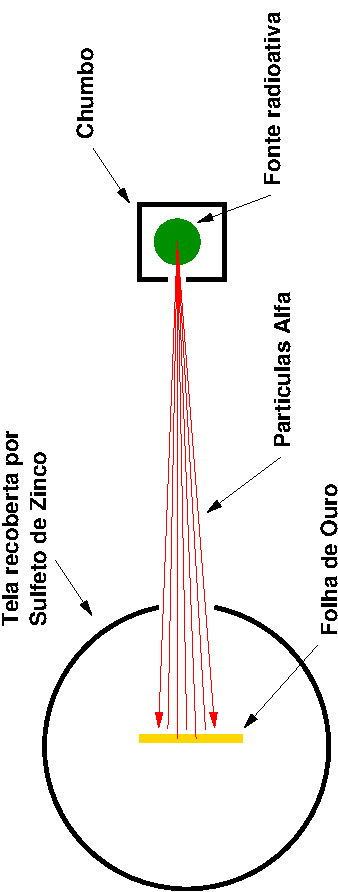
\includegraphics[scale=0.9,angle=-90]{rutherford}
\end{center}
\caption[O \eng{setup} de Rutherford.]{A configuração do experimento de
Rutherford para a constatação de que o núcleo atômico era denso e
positivo. Extraída de \cite{partadv}.}
\label{fig:rutherford}
\end{figure}

Os \idx{nêutrons}, os constituintes nucleares de carga neutra, foram
descobertos em 1932 por Chadwick. Planck e Bohr entre outros físicos
desenvolveram as teorias quânticas para explicar várias anomalias
experimentais, introduzindo o conceito de níveis (ou \idxeng{quanta}) de
energia. Em 1925, Heisenberg e Schrödinger formularam a \idx{Mecânica
Quântica}, que sintetizou o formalismo matemático que substituiu a dinâmica de
Newton. Nesta área, os resultados de medidas físicas são de natureza
inerentemente probabilística. A teoria modela o cálculo destas probabilidades
e, de forma bem-sucedida, descreve o comportamento da matéria em pequenas
escalas.

A mecânica quântica tam\-bém fornece ferramentas te\-ó\-ri\-cas para a
fí\-si\-ca de ma\-té\-ria condensada, que estuda o comportamento físico de
sólidos e líquidos, incluindo fenômenos de cristalização, semi-condutividade e
super-condutividade.

A \idx{Teoria Quântica dos Campos} foi formulada para estender a mecânica
quântica fazendo-a consistente com a relatividade especial, atingindo sua
forma moderna no final dos anos 40 com o trabalho de Feynman, Schwinger,
Tomonaga e Dyson. Eles formularam a \idx{Eletrodinâmica Quântica}, que
descreve a interação eletromagnética.

A teoria quântica dos campos fornece o ferramental de fundo para a fí\-si\-ca
de par\-tí\-cu\-las moderna, que estuda primordialmente as forças elementares
entre as partículas. Em 1954, Yang e Mills desenvolveram uma classe de teorias
de Gauge, introduzindo o \idx{Modelo Atômico Padrão} ou simplesmente
\idx{Modelo Padrão}, que foi completado nos anos 70. O Modelo Padrão descreve
de forma bem-sucedida quase todas as partículas elementares observadas até
hoje e abrange as \idx{forças fundamentais} ``forte'', ``fraca'' e
``eletromagnética'' assim como as partículas de que se compõe toda a matéria
conhecida. O Modelo Padrão não é, no entanto, uma teoria fundamental de todas
a interações existentes na natureza, primariamente por não descrever a
gravidade.

\section{Física de Partículas Moderna}

Embora de grande sucesso, modelando resultados encontrados
ex\-pe\-ri\-men\-tal\-men\-te, o Modelo Pa\-drão nunca foi aceito como uma
teoria completa de física fundamental. Isto acontece por causa de dois
aspectos:

\begin{enumerate}
\item O modelo contém 19 parâmetros livres, como a massa das partículas, que
  precisam ser determinados experimentalmente (e mais outros 10 para massas de
  neutrinos). Estes parâmetros não podem ser calculados independentemente;

\item O modelo não descreve a interação gravitacional;
\end{enumerate}

Desde a finalização do Modelo Padrão, muitos esforços foram travados para
resolver ambos os pontos. Um deles é conhecido como a \idx{Grande Unificação},
do qual muitos aspectos estão bastante longe de serem observados em
laboratório. O bóson de Higgs\index{bóson de Higgs}, que é previsto pelo
modelo padrão, ainda não foi observado até os dias de hoje. Alguns
experimentos, dentre os quais o experimento \idx{ATLAS} (do inglês, \eng{A
Toroidal LHC Apparatus}) no \idx{CERN}, Suíça, estão sendo construídos para o
estudo desta física.

\subsection{Aceleradores e Detetores}

De forma parecida a Rutherford, os físicos atuais usam um feixe de partículas
aceleradas para recriar em laboratório condições que permitam o estudo das
interações sub-atômicas que se deseja averiguar. Estes feixes podem colidir com
um alvo fixo ou com um outro feixe de partículas, que é acelerado em direção
contrária ao feixe primário. Para visualizar eletronicamente os sub-produtos
de tais interações físicas, utilizam-se múltiplos detetores.

A aceleração das partículas resolve dois problemas que os físicos de hoje
encontram em seus experimentos:

\begin{enumerate}
\item Comprimento de Onda - O comprimento de onda determina a acurácia do que
é possível observar \cite{partadv}.

Uma vez que as par\-tí\-culas tam\-bém apresentam caracte\-rís\-ticas de onda,
não é pos\-sí\-vel obter uma medida acurada usando-se partículas comuns, como
um e\-lé\-tron, na observação de partículas muito pequenas. Um elétron não
serve, nem mesmo, para observar outro elétron. A aceleração da partícula, no
entanto, aumenta seu momento, diminuindo\footnote{O comprimento de onda
($\lambda$) e o momento ($p$) de um corpo são inversamente proporcionais -
$p=h/\lambda$.} seu comprimento de onda e permitindo que medidas acuradas
possam ser tomadas, usando-se partículas maiores, como léptons.

\item Energia Cinética - Deseja-se, nos experimentos modernos, que o impacto
seja o mais aniquilador possível. Isto é interessante, pois ao se aniquilar
matéria, liberando muita energia, partículas mais massivas e menos estáveis são
geradas. Ao se acelerar uma partícula, aumenta-se sua energia cinética,
tornando a colisão com o alvo mais eficiente.
\end{enumerate}

\subsection{A Aceleração das Partículas}

A aceleração de partículas \index{aceleração de partículas} é um processo
bastante simples: inicialmente devem-se escolher partículas eletricamente
carregadas para um experimento - e\-lé\-trons, pró\-tons ou íons são
utilizados normalmente. As par\-tí\-culas eletricamente carregadas são
posicionadas no interior de um túnel e aceleradas por pulsos
eletromagnéticos\index{pulsos eletromagnéticos} (e.m). A
Figura~\ref{fig:acelera} exemplifica como elétrons possam ser acelerados: as
ondas e.m. aceleram as partículas, pois elementos eletricamente carregados
adquirem força (aceleração) quando envoltos por um campo eletromagnético.

\begin{figure}
\begin{center}
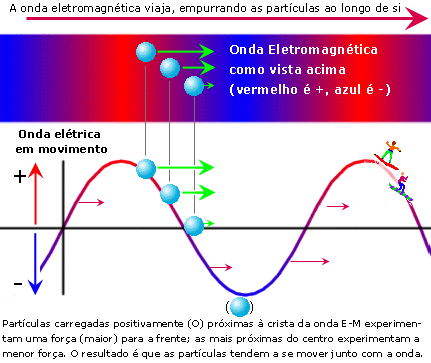
\includegraphics[scale=0.7]{static-wave}
\end{center}
\caption[A aceleração de partículas.]{A aceleração de partículas eletricamente
carregadas usando-se de pulsos e.m.. Extraído de \cite{partadv}.}
\label{fig:acelera}
\end{figure}

Os aceleradores podem ter dois formatos\index{acelerador!tipos}: linear e
circular. Num acelerador linear\index{acelerador!linear}, as partículas são
injetadas em uma extremidade e percorrem uma reta até que colidam com outras
partículas ou com um alvo fixo. A outra possibilidade é ter um acelerador
circular ou
síncrotron\index{acelerador!circular}\index{acelerador!síncrotron|see{acelerador
circular}}. Num acelerador circular, as partículas são injetadas em um ponto
do anel de aceleração e lá permanecem até que tenham adquirido velocidade
suficiente ao experimento a que se destinam. A aceleração circular exige que
ímãs poderosos curvem a trajetória das partículas injetadas. Aceleradores
circulares também permitem que vários experimentos sejam conduzidos em pontos
de sua circunferência, de forma simultânea.

\subsection{Deteção: Vendo o que ocorreu a\-pós a coli\-são}

Depois de um acelerador ter ``bombeado''\ energia suficiente para suas
par\-tí\-culas, estas são colocadas em rota de colisão com um alvo fixo ou,
então, com as partículas de um outro feixe acelerado. Cada uma dessas colisões
forma um \emph{evento} físico. O objetivo dos físicos é isolar cada evento,
coletar dados a seu respeito e verificar se o processo do qual a partícula
participou está de acordo com a teoria que está sendo testada no experimento
em questão.

A análise de cada evento pode ser bastante complexa, já que muitas (sub)
par\-tí\-cu\-las podem ser produzidas. A maioria dessas partículas têm tempo
de vida tão curto que viajam por distâncias extremamente curtas, antes de
decaírem em outras partículas, sem deixarem pistas aparentemente detetáveis.

Para procurar esses vários objetos e os produtos de seus decaimentos, os
físicos projetam detetores com multi-componentes, que testam diferentes
aspectos de um evento \cite{d0, cms, atlas-tp, booth}. Cada componente de um
detetor moderno é usado para medir vários parâmetros das partículas
provenientes de um evento, e/ou distinguir os diferentes tipos de objetos
gerados.  Quando todos esses componentes funcionam juntos para detetar um
evento, partículas individuais podem ser distinguidas da multidão para efeito
de análise e o evento original pode ser reconstruído.

Seguindo cada evento, os sistemas de processamento coletam e interpretam a
vasta quantidade de dados dos detetores e apresentam os resultados extrapolados
aos físicos.

Os físicos interessam-se pelos eventos que ocorrem durante ou mesmo depois da
colisão das partículas. Por essa razão, colocam detetores em regiões nas quais
os objetos resultantes daquela interação passarão. Os detetores são construídos
de diferentes maneiras, dependendo do tipo de colisão analisada:

\begin{description}
\item[Alvo fixo] Num experimento envolvendo um alvo fixo, as partículas
produzidas geralmente projetam-se para frente; por isso, os detetores são na
forma de cones e são colocados ao longo da direção do feixe;

\item[Feixes de colisão] Durante um experimento envolvendo feixes em
co\-li\-são, as par\-tí\-cu\-las são espalhadas em todas as direções; assim, o
detetor mais adequado é esférico ou, mais comumente, cilíndrico.
\end{description}

\subsubsection{Composição dos Detetores}

Os detetores modernos são feitos de peças distintas, que testam diferentes
aspectos de um evento. Esses vários componentes são organizados de tal maneira
que os físicos possam obter o máximo de informação sobre as partículas geradas
durante um evento. A Figura~\ref{fig:modern-detect} mostra um diagrama
esquemático de um pequeno detetor cilíndrico moderno. Uma figura humana é
mostrada em escala, indicando as grandes proporções dos detetores típicos em
Física de Altas Energias.

\begin{figure}
\begin{center}
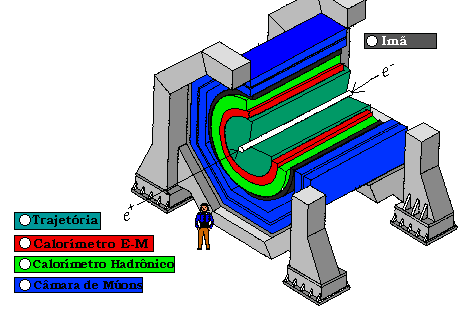
\includegraphics[scale=0.7]{modern_detect}
\end{center}
\caption{O diagrama de um detetor cilíndrico moderno. Extraído de \cite{partadv}.}
\label{fig:modern-detect}
\end{figure}

Na Figura~\ref{fig:modern-detect}, é possível observar que um detetor moderno
é composto, basicamente, de 4 sub-detetores principais. O primeiro detetor, de
dentro para fora (tomando o feixe de partículas como origem), tem a função de
determinar a rota e curvatura de partículas, por isto é chamado de detetor de
trajetória, arrasto ou, mais comumente, traços. A curvatura das partículas
sobre o campo magnético a que são expostas no detetor dá informações sobre a
carga da partícula e seu momento. O segundo detetor é chamado calorímetro
eletromagnético (e.m.) e tem a função de determinar a energia total de
elétrons, pósitrons e fótons (raios $\gamma$). Estas partículas interagem com
este detetor, originando chuveiros compostos de outros elétrons, pósitrons e
fótons. O terceiro detetor, o calorímetro hadrônico, mede a energia total de
chuveiros originados por hádrons (prótons, nêutrons ou mésons). No caso de
partículas hadrônicas, este chuveiro é mais largo e profundo que o equivalente
para partículas como elétrons e fótons. O quarto detetor é um detetor de
múons. Somente estas partículas e neutrinos escapam dos outros sistemas de
deteção. Neutrinos, infelizmente, nem por este último são detetados. Sua massa
pode ser estimada, no entanto, através da energia faltante no evento
\cite{atlas-tp}. A Figura~\ref{fig:decay} mostra como alguns tipos de
partículas interagem com estes detetores. Fótons, por exemplo, têm carga nula
e não são detetados pelos detetores de traços, mas interagem com os
calorímetros e.m.. Elétrons e pósitrons interagem tanto com os detetores de
traços quanto com o calorímetro e.m., desenvolvendo cascata e.m. neste
último. Prótons são detetáveis pelos detetores de traços, mas desenvolvem
cascata somente nos calorímetros hadrônicos. Nêutrons somente desenvolvem
cascata nos detetores hadrônicos.

\begin{figure}
\begin{center}
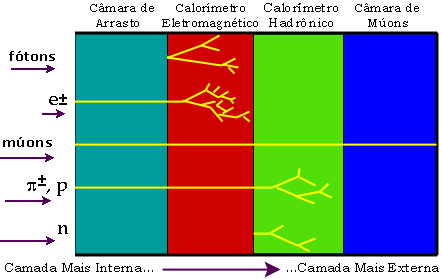
\includegraphics[scale=0.6]{decay_chart}
\end{center}
\caption{A interação de partículas com os detetores modernos. Extraído de
\cite{partadv}.} 
\label{fig:decay}
\end{figure}

\section{Calorimetria Moderna}
\index{Calorimetria}
\label{sec:calorimetria}

\idx{Calorímetros} são detetores compostos utilizando a absorção
total de partículas para medir a energia e a posição de partículas e
jatos. Durante o processo de absorção, chuveiros são gerados por cascatas de
interações. Durante a formação do chuveiro, eventualmente, a maior parte da
massa da partícula será convertida em radiação ionizante, o que explica o nome
deste tipo de detetor. É claro, nenhuma temperatura é medida, mas as
características de interação com a matéria (e.g. excitação atômica, ionização)
são utilizadas para gerar um efeito detetável, através de partículas
carregadas. A calorimetria é também uma forma de detetar e medir partículas
neutras entre as secundárias produzidas em uma colisão de altas energias
\cite{bock:detector}.

Estes detetores são normalmente construídos tendo por base diferentes
sub-detetores e têm seu desempenho otimizado para as diferentes partículas que
incidirão sobre seu corpo. Cada sub-detetor de um calorímetro é por sua vez
formado por múltiplas células de deteção, que medem a energia das partículas
que interagem por seu volume. As células são alinhadas para formar torres
tipicamente na direção de incidência. A análise da energia depositada nas
células e torres permite medir o perfil lateral e longitudinal das cascatas e
daí sua geometria ser otimizada para este propósito.

Tipicamente, \idx{partículas eletromagnéticas} incidentes (i.e. elétrons e
fótons) são completamente absorvidos em calorímetros eletromagnéticos, a
primeira das camadas de calorímetros compostos. Sua construção aproveita-se da
geometria de chuveiros eletromagnéticos, que são compactos e curtos, para
medir a energia e posição com precisão ótima para as partículas, que
incluem $\pi^{0}$'s, que decaem eletromagneticamente.

\idx{Hádrons} incidentes (prótons, nêutrons, etc.), diferentemente,
podem começar sua interação no calorímetro eletromagnético, mas quase sempre
só serão completamente absorvidos em camadas posteriores, i.e. em
\idx{calorímetros hadrônicos}, construídos exatamente para conterem estes
chuveiros. Chuveiros hadrônicos têm formato bastante diversificado.

A qualidade da discriminação entre chuveiros eletromagnéticos e hadrônicos, é
um critério importante para um calorímetro. É importante conter chuveiros
eletromagnéticos em um espaço mais curto, sem que se inicie um grande número
de chuveiros hadrônicos.

Calorímetros também provêm assinaturas para partículas que não são absorvidas:
\idx{múons} e \idx{neutrinos}. Múons não formam chuveiro na matéria, mas sua
carga deixa um sinal de ionização, que pode ser identificado em um calorímetro
se a partícula está suficientemente isolada (e a eletrônica associada
permitir), e ser associado a um traço detetado nos detetores de traço e/ou no
detetor de múons. Neutrinos, por outro lado, não deixam sinais em um
calorímetro, mas sua existência pode ser, algumas vezes, inferida através do
princípio da conservação de energia: num calorímetro hermeticamente fechado,
ao menos um neutrino suficientemente energético ou grupo de neutrinos pode ser
observado tomando-se a soma vetorial de todos os outros momentos medidos, e a
soma da energia observada em cada célula do calorímetro. A precisão de tais
métodos, usualmente limitada à direção transversal, requer um vazamento mínimo
de energia em todas as direções e daí o desafio para o projeto de calorímetros
na prática.

\subsection{Tipos de Calorímetros}

Quanto à construção, é possível se distinguir os seguintes tipos de
calorímetro \cite{bock:detector, hadcal}:

\begin{itemize}
  \item \textbf{Homogêneos:}\index{Calorímetro!Homogêneo} Em calorímetros
  deste tipo, as funções de absorção e geração e leitura de sinais são
  combinadas em um único tipo de material. Estes materiais são quase que
  exclusivamente usados para calorímetros eletromagnéticos, por exemplo
  cristais (vidros dopados com chumbo), materiais compostos ou gases nobres em
  estado líquido;

  \item \textbf{Heterogêneos:}\index{Calorímetro!Heterogêneo} Tam\-bém
  conhecidos como \idx{ca\-lo\-rí\-me\-tros de amostragem}. Neste tipo de
  detetor, as fun\-ções de ab\-sor\-ção de energia e leitura do sinal são
  separadas. Isto permite uma escolha ótima do material de absorção e
  liberdade no tratamento do sinal. Calorímetros heterogêneos são, em sua
  maior parte, construídos como sanduíches (e.g. chumbo, aço e ferro),
  alternando estes materiais com camadas de material ativo (e.g. cintiladores
  líquidos, sólidos ou contadores proporcionais). Somente parte da energia do
  chuveiro absorvida pelo material ativo é medida. Calorímetros hadrônicos,
  necessitando de uma profundidade considerável e largura para criar e
  absorver os chuveiros, são necessariamente deste tipo (veja a
  Seção\ref{sec:calohad}).

  Ainda que o desempenho não dependa fortemente da orientação, a espessura não
  pode variar em demasiado para assegurar uma resolução independente da
  direção e da posição dos chuveiros.
\end{itemize}

A calorimetria moderna é a arte de escolher entre duas restrições
conflitantes; a principal é normalmente formulada em termos da resolução em
energia, coodernadas espaciais, capacidade de filtragem, resistência à
radiação dos materiais usados e em parâmetros eletrônicos como a faixa de
operação e a extração de sinais. Na maior parte dos casos, o custo final de
produção, a segunda restrição, é o parâmetro mais limitante. O número de
soluções em calorimetria é maior para calorímetros do que para detetores de
traços, e soluções bastante engenhosas foram encontradas nos últimos 15 anos
\cite{hadcal}.

\subsection{A Física da Calorimetria}

A acurácia das medidas de energia em calorímetros aumenta com o aumento da
energia de partículas incidentes \cite{hadcal}, de acordo com a fórmula
empírica:

\begin{equation}
  \frac{\sigma_{E}}{E} \approx \frac{a}{\sqrt{E}} + b
\end{equation}

Onde $E$ é a energia da partícula incidente e $\sigma_{E}$ representa o desvio
padrão da medida de energia e $a$ e $b$ são constantes que dependem do tipo de
detetor, e.g. sua espessura e características das camadas ativas e passivas.

\subsubsection{Calorimetria eletromagnética}
\index{Calorimetria!eletromagnética}

Partículas eletromagnéticas perdem energia através de dois processos durante a
interação com calorímetros:

\begin{itemize}
\item {\bf radiação:} através do fenômeno conhecido como
  \idxeng{Bremsstrahlung}, onde a partícula incidente muda de rota, perdendo
  energia e gerando um fóton. Este fóton seguirá um caminho de interação
  independente do elétron original, possivelmente através de espalhamento
  Compton, efeito foto-elétrico ou produção de pares elétron-pósitron,
  dependendo diretamente da energia com o qual foi gerado. Os elétrons
  remanescentes deste processo, se tiverem energia, poderão repetir este
  processo até que as partículas formadas não possam mais irradiar. Esta
  energia limite é conhecida como \idx{Energia Crítica} ($\varepsilon_{c}$) e
  depende do peso atômico (Z) do material por onde se desenvolve a cascata
  eletromagnética. Valores típicos de $\varepsilon_{c}$ estão na faixa de
  dezenas de MeV (exemplo: $\varepsilon_{c}(Cu) = 25$ MeV). Quanto maior o
  número atômico, maiores as chances de perda por radiação\cite{knoll, leo}.

\item {\bf ionização:} interagindo com os elétrons do material em que viaja a
  partícula, ionizando-o e desta forma perdendo energia.
\end{itemize}

Por estas razões, chuveiros eletromagnéticos são curtos e bem contidos em
calorímetros pouco espessos. A cascata desenvolve-se a partir do eixo de
penetração da par\-tí\-cu\-la, de forma aproximadamente isotrópica, num espaço
de tempo extremamente curto, na ordem de centenas de picossegundos.

A Figura~\ref{fig:cms-ecal} mostra um diagrama esquemático em três dimensões
da seção eletromagnética do calorímetro do experimento \idx{CMS} (do inglês
\idxeng{Compact Muon Solenoid}) no CERN, Suíça. Este calorímetro em formato
cilíndrico é feito de cristais compostos. Na cavidade central deste aparato
encaixam-se os detetores de traço do experimento. A segmentação do detetor é
indispensável para a localização de objetos no espaço.

\begin{figure}
\begin{center}
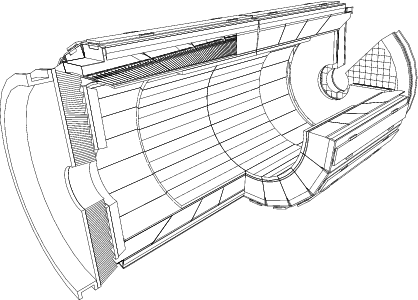
\includegraphics[scale=0.8]{cms-ecal}
\end{center}
\caption{Diagrama da seção eletromagnética do calorímetro do experimento CMS.}
\label{fig:cms-ecal}
\end{figure}

\subsubsection{Calorimetria hadrônica}
\index{Calorimetria!hadrônica}
\label{sec:calohad}

O chuveiro hadrônico é dominado por uma sucessão de interações inelásticas
deste tipo. Em altas energias, estas são caracterizadas pela produção de
partículas múltiplas e pela emissão de partículas originárias de decaimentos
nucleares do material excitado. Devido a freqüente geração de $\pi^{0}$'s
(diz-se ``pi-zeros'', ou seja, píons que não possuem carga elétrica),
chuveiros hadrônicos têm também componentes eletromagnéticas.

Quando um hádron altamente ener\-gé\-tico penetra num bloco de ma\-té\-ria,
ele, em algum ponto, interagi\-rá com algum nú\-cleo atômico. Neste processo,
mésons são usualmente gerados (píons, káons, etc.). Outra fração da energia
inicial da partícula é transferida para o núcleo com o qual o hádron
interagiu. Este núcleo excitado, liberará esta energia emitindo um certo
nú\-mero de nú\-cleons (prótons ou nêutrons) e num estado posterior,
$\gamma$'s de baixa energia, perdendo sua energia cinética por ionização. As
partículas produzidas nesta reação (mésons, núcleons e $\gamma$'s), por sua
vez, podem perder sua energia cinética por ionização ou induzir novas reações
formando uma cascata ou chuveiro \cite{hadcal}.

Limites intrínsecos na resolução em energia de calorímetros hadrônicos são
\cite{hadcal}:

\begin{itemize}
  \item Uma componente $\pi^{0}$, flutuante dentre os chuveiros secundários, que
  interaja eletromagneticamente sem qualquer outra interação nuclear ($\pi^{0}
  \rightarrow \gamma\gamma$). A fração de $\pi^{0}$'s é dada por
  $\frac{\pi^{0}}{all} \approx 0,10 \log{E}$, $E$ em GeV. Chuveiros hadrônicos
  podem desenvolver uma componente eletromagnética dominante;

\item Uma boa parte da energia disponível é convertida em excitação e quebra
  de núcleos atômicos. Somente uma pequena fração desta energia aparecerá como
  sinal detetável, havendo largas flutuações evento-a-evento. Estas flutuações
  podem ser compensadas com a boas escolhas dos materiais ativos e absorvedores
  do detetor;

\item Uma fração considerável da energia da partícula incidente é despendida
  em reações que não resultarão em sinal observável, tais como vazamento de
  energia em várias formas (evaporação ou quebra nuclear, excitação nuclear,
  etc.).
\end{itemize}

De forma contrária a chuveiros eletromagnéticos, que se desenvolvem num curto
espaço de tempo, chuveiros hadrônicos são caracterizada por diferentes escalas
de tempo. Os fenômenos mais lentos podem durar de centenas de nanossegundos a
um microssegundo.

Sumarizando:

\begin{enumerate}
\item Calorímetros são sensíveis a partículas neutras e carregadas;

\item Devido a diferenças na forma de deposição de energia das partículas, a
identificação de partículas com alta eficiência pode ser atingida usando-se
calorímetros;

\item Quanto maior a energia da partícula, mais acurado é o resultado. Isto não
acontece com outros tipos de detetores;

\item Para conter o desenvolvimento de cascatas dos objetos a serem medidos, a
profundidade dos calorímetros aumenta logaritmicamente com a energia, o que
permite o projeto de detetores mais compactos;

\item Não precisam de campos magnéticos (como os detetores de traços);

\item Podem ser segmentados, o que permite acurada medida da energia e a
visualização da tra\-je\-tó\-ria das par\-tí\-cu\-las;

\item Resposta rápida (melhor que 50 ns) pode ser atingida, o que é importante
num ambiente com alta taxa de eventos;

\item A informação de energia pode ser usada para filtrar eventos interessantes
com alta seletividade;
\end{enumerate}

\section{Sistemas de Filtragem}
\index{Sistemas de Filtragem}
\label{sec:trigger}

Os sinais detetados por calorimetria são normalmente utilizados como fonte de
discriminação rápida de eventos interessantes em experimentos modernos. Um
Sistema de Filtragem, ou \idxeng{Trigger}, é um conjunto de dispositivos,
normalmente uma combinação de componentes eletrônicos e computadores, provendo
um sinal rápido quando a física interessante acontece
\cite{bock:detector, cms-trigger, d0-trigger, d0-trigger2, hlt-tdr,
trig-review}. Tipicamente, um sistema de filtragem está associado a
experimentos com detetores e seus sinais ativam o sistema de gravação de
eventos para registrar parte ou a totalidade dos impulsos captados em mídia
permanente. As condições que levam o sistema de filtragem a produzir o sinal
de aceitação são comumente chamadas de
\idx{assinaturas do evento}. As condições podem ser tão simples quanto
identificar um traço gerado por uma partícula carregada passando por
cintiladores durante um período de tempo, ou tão complexos quanto o critério
de massa efetiva entre léptons identificados que devam satisfazer colisões de
altas energias.

Em muitos experimentos, a aquisição de dados, através do \idx{tempo morto} que
causa, é um fator crítico determinante, que limita as estatísticas e o
potencial físico. Um sistema de filtragem eficaz é então o ponto-chave para a
transmissão de dados que têm alta probabilidade de conter física de interesse
e rejeição, com base nas possibilidades de deteção, de todos ou da maioria dos
eventos que representem física ordinária e trivial. Claramente, não somente a
eletrônica e informática do sistema de filtragem são necessárias ao trabalho,
mas também os dados carregados pelo sistema de leitura do detetor, que provêm
as informações que serão averiguadas pelo primeiro.

Dependendo do acelerador utilizado, sistemas de filtragem podem ser chaveados
(e.g. por pacotes de partículas chegando ao ponto de colisão) ou
permanentemente ativados (como para o estudo de raios cósmicos). As
implementações podem ser síncronas ou operar em tempo real, ou ainda
se comporem de vários circuitos assíncronos operando paralelamente,
respeitando uma unidade de controle central (que também tem a função de
re-sincronizar o sistema como um todo). As implementações nos dias de hoje vão
desde simples portas E/OU até \idxeng{Field-Programmable Gate Arrays} ou
\idx{FPGA}'s. Os tempos de retardo dependem do volume dos dados a serem
analisados (e comumente na ocupação de recursos de processamento a que se
destinam). Algoritmos de filtragem também podem ter seu desempenho variando no
tempo já que dependem da complexidade dos objetos em análise.

Em grandes experimentos, sistemas de filtragem são implementados em múltiplos
níveis, tipicamente consistindo de um primeiro nível síncrono, que identifica
candidatos a partir de um subconjunto dos dados colhidos pelos detetores,
reduzindo a taxa de eventos por algum fator. Subseqüentemente, os dados são
digitalmente transmitidos para \idx{bancos de memória} (do inglês
\idxeng{buffers}) e para um segundo nível de filtragem, normalmente assíncrono,
onde algoritmos mais complexos, baseados em um conjunto de dados mais
completo, conseguem reduzir novamente a taxa de eventos. Eventualmente,
depois de uma terceira ou quarta iteração, o evento é gravado em mídia
permanente.

\subsection{Sistemas de filtragem em experimentos modernos}

Um experimento em Física de Altas Energias como o DZERO \cite{d0}, localizado
no FermiLab, próximo a Chicago nos Estados Unidos, é um exemplo de um
experimento com um sistema de filtragem moderno. O cruzamento de pacotes de
prótons e anti-prótons que geram as colisões a serem estudadas ocorrem numa
taxa de 2,5 MHz (ou seja, 2,5 milhões de colisões por segundo). Cada colisão
poderá produzir um evento que possui 0,25 \eng{megabytes} em dados. Se a taxa
total fosse escrita em fitas magnéticas\footnote{Este tipo de tecnologia ainda
é atualmente utilizado para a armazenagem de grandes quantidades de dados ($>
10^{2} Terabytes$).}, assumindo um custo de 40 centavos de dólar por
\eng{Gigabyte}, o custo total seria de 10,5 milhões de dólares por ano. No 
entanto, a maior parte das colisões de pacotes contém interações elásticas ou
até mesmo nulas. Para tirar proveito desta natureza, o experimento DZERO
emprega um sistema de filtragem em múltiplos níveis para reduzir a taxa de
eventos registrada a 50 Hz, implicando em um custo aproximado de 75.000
dólares por ano em fitas magnéticas.

É claro que a economia em fitas magnéticas não é a única razão da existência
de um sistema de filtragem. Planejar e projetar um sistema de aquisição de
dados com uma taxa de dados de 600 \eng{gigabytes} por segundo seria
proibitivo economicamente, especialmente considerando-se o valor relativo dos
dados coletados. Os atuais programas de reconstrução de eventos também
consomem grande poder de processamento e, se a entrada puder ser sensivelmente
reduzida em volume, menor a quantidade de recursos computacionais serão
necessários para a análise \eng{offline}.

O enfoque usado para projetar e implementar um sistema de filtragem depende
fortemente do domínio do problema. Um experimento moderno em Física de Altas
Energias deve estar apto a responder a um novo evento, em geral, a cada
dezena ou dezenas de nanossegundos. O \idx{tamanho do evento} para grandes
experimentos (veja a Figura~\ref{fig:eventsize}) também tende a ser grande,
chegando a alguns \eng{megabytes} por evento em alguns dos experimentos do
\idx{LHC} (\idxeng{Large Hadron Collider}).

\begin{figure}
\begin{center}
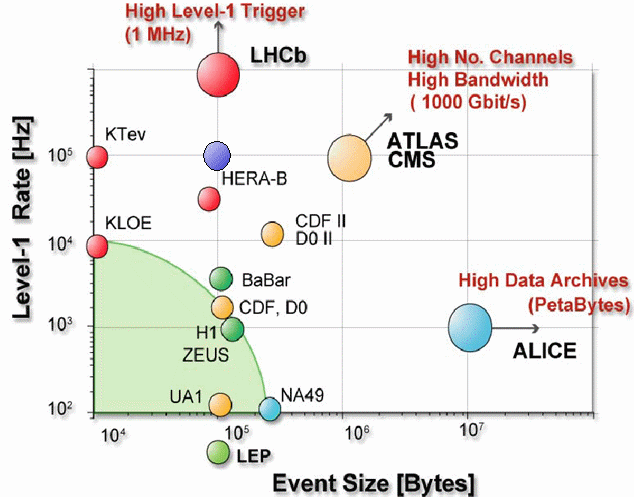
\includegraphics[scale=0.6]{eventsize}
\end{center}
\caption{O tamanho do evento \eng{versus} a taxa de produção em experimentos
atuais. Extraído de \cite{trig-review}.}
\label{fig:eventsize}
\end{figure}

Experimentos modernos usam um sistema de filtragem dividido em múltiplos
níveis para endereçar o problema das taxas de entrada. Os níveis mais baixos
implementam algoritmos simples e rápidos, normalmente usando FPGA's e
\eng{hardware} personalizado, que rejeitem os processos (\eng{background})
mais simples e abundantes. Os níveis mais altos são progressivamente mais
sofisticados e também requerem mais tempo para atingir níveis de rejeição
aceitáveis. Ademais, carregando uma menor quantidade ou qualidade de dados nos
níveis iniciais de filtragem, estes experimentos conseguem reduzir o fluxo de
informação no sistema de leitura: tão logo um evento seja rejeitado, seus
dados são descartados.

Classicamente, o nível em \eng{hardware} é chamado de \idx{Primeiro Nível}. O
seguinte, composto de partes personalizadas em \eng{hardware} e computadores,
é chamado de \idx{Segundo Nível}. O último estágio, chamado de
\idx{Terceiro Nível}, composto normalmente de redes de computadores
tipo PC, realiza a classificação final. Comumente o segundo e terceiro níveis
de filtragem são conhecidos como \idx{Filtros de Alto Nível} ou
\idxeng{High-Level Triggers}, \idx{HLT}.

%% Hello emacs, this is -*- latex -*-
\typeout{ ====================================================================}
\typeout{ This is file atlas.tex, created at 13-Feb-2004 }
\typeout{ Maintained by Andre DOS ANJOS <Andre.dos.Anjos@cern.ch> }
\typeout{ ====================================================================}

\chapter{O Experimento ATLAS no CERN}
\label{chap:atlas}

% advocate: CERN um centro de grandes pesquisas e pesquisadores.
% Alguns Premios Nobel foram executados no CERN, o que o classifica como
% um grande centro de pesquisa.

O experimento \idx{ATLAS} � um dos 4 experimentos que est�o sendo constru�dos
ao redor do super-acelerador e colisionador de part�culas \idx{LHC} (do ingl�s
\idxeng{Large Hadron Collider}), no Laborat�rio Europeu para a F�sica de
Part�culas - \idx{CERN} em Genebra, Su��a \cite{atlas-tp}. O \idx{CERN} � um
dos maiores, sen�o o maior laborat�rio para a F�sica de Altas Energias na
atualidade, conduzindo v�rios experimentos em regime de colabora��o
internacional. A pr�xima se��o introduz um pouco de sua hist�ria, que culmina
na aprova��o para cria��o do LHC e dos 4 grandes experimentos montados a
partir de sua infraestrutura.

\section{O Laborat�rio CERN}

O CERN surgiu em 1952 quando, depois de v�rias reuni�es, 11 Estados europeus
aceitaram organizar um Conselho Europeu para a Pesquisa Nuclear (do franc�s
\idxfr{Conseil Europ�en pour la Recherche Nucl�aire}) Provis�rio, com sede
prevista em um local pr�ximo � Genebra, na Su��a. Dois anos ap�s a ratifica��o
de uma convers�o por seus \idx{Estados-Membro}, no dia 29 de Maio de 1954, o
centro era inaugurado. Embora o termo ``Provis�rio'' tenha sido banido do nome
do laborat�rio, a sigla CERN continuou a ser empregada.
 
O primeiro acelerador do CERN\index{CERN!primeiro acelerador}, um
\idxeng{Synchro-Cyclotron} de pr�tons a 600 MeV, come�ou a operar em
1957. Este acelerador foi respons�vel pela obten��o do primeiro resultado
experimental do laborat�rio: a observa��o do decaimento de um p�on em um
el�tron e um neutrino. Em 1959, a primeira ``grande'' m�quina do CERN j�
estava em opera��o. Era um \idxeng{Proton Synchrotron} (PS) de 28 GeV - o
acelerador de maior energia na �poca.

Algumas das tecnologias para colis�o e dete��o de part�culas existentes nos
dias de hoje foram inventadas neste laborat�rio. Dentre as principais, podemos
destacar:

\begin{itemize}
\item \idx{T�cnica de Resfriamento Estoc�stico} (do ingl�s
\idxeng{Stochastic Cooling Technique}), proposta por Simon van der Meer em
1968;

\item as \idx{C�maras Proporcionais Multifio} (do ingl�s
\idxeng{Multiwire Proportional Chambers}) e as \idx{C�maras de Arrasto} (do
ingl�s \idxeng{Drift Chambers}). A cria��o desta tecnologia daria o Pr�mio
Nobel a Georges Charpack em 1992;
\end{itemize}

Outras tecnologias associadas tamb�m tiveram destaque. Por exemplo, em 1990,
Tim Berners-Lee, trabalhando em conjunto com Robert Cailliau, prop�s um
sistema de informa��o distribu�da, baseado em ``hipertextos'', uma forma de
descrever liga��es a documentos guardados em computadores. Escondendo o
endere�o de rede atrav�s de �tens grafados na tela, a informa��o pode ser
ligada atrav�s de v�rios computadores. O nome \idx{Word-Wide Web} foi
escolhido na ocasi�o.

A inje��o de fundos para a pesquisa nuclear alavancou a cria��o de uma grande
infra-estrutura de an�is de acelara��o e estocagem de part�culas na d�cada de
60, dos quais o mais importante aparato foi o \idxeng{Super Proton
Synchrotron} (\idx{SPS}), que come�ou a operar em 1976 com energia inicial de
300 GeV. O SPS t�m 7 km de extens�o e atravessa a fronteira franco-su��a nos
arredores de Genebra, tendo sido o maior instrumento cient�fico da �poca.  A
hist�rica descoberta dos b�sons W e Z em janeiro e maio de 1983
respectivamente ficou por conta dos trabalhos no SPS, confirmando a
\idx{teoria eletrofraca}, que unificava as for�as fraca\index{for�a fraca} e
eletromagn�ticas\index{for�a eletromag�tica}. Carlo Rubia e Simon van der Meer
receberam o pr�mio Nobel por este trabalho em 1984. Este trabalho motivou a
constru��o do \idx{Grande Colisionador El�tron-P�sitron} (do ingl�s
\idxeng{Large Electron-Positron Collider}, \idx{LEP}), com energia incial
prevista para 50 GeV. O LEP estudaria em detalhes as part�culas Z em quatro
experimentos simult�neos.

Os anos de 1989 a 1994 foram marcados pelo sucesso dos experimentos no LEP. O
resultado mais impressionante se deu com a precisa medi��o dos par�metros de
resson�ncia da part�cula Z: os 4 experimentos do LEP reconstru�ram mais de 10
milh�es de deca�mentos desta part�cula no per�odo. Com base nestes resultados,
o Conselho dos Estados-Membro aprovou a constru��o do \idx{Grande Colisionador
de H�drons} (do ingl�s \idxeng{Large Hadron Collider}, LHC). A
Figura~\ref{fig:accel} mostra o atual conjunto de aceleradores do CERN e suas
interconex�es.

\begin{figure}
\begin{center}
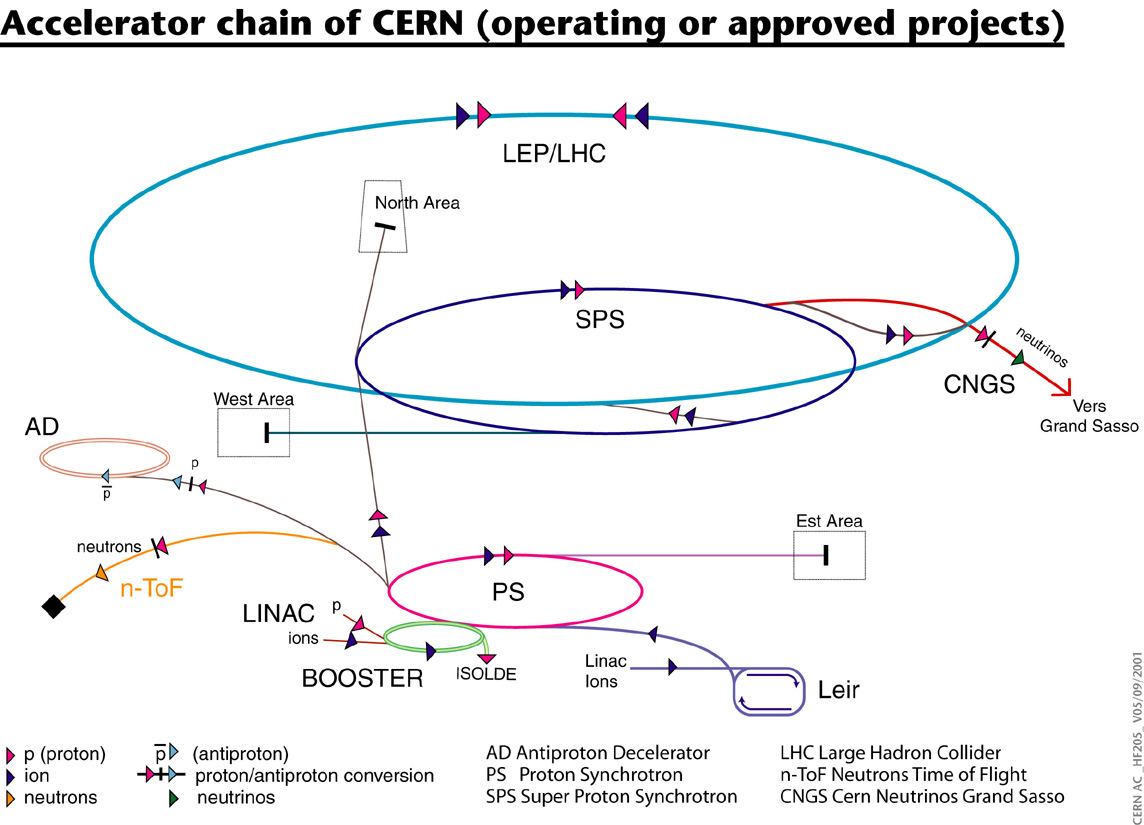
\includegraphics[scale=0.74]{accelerators}
\end{center}
\caption{Diagrama esquem�tico dos aceleradores do CERN e suas conex�es.}
\label{fig:accel}
\end{figure}

\section{O LHC}

No LHC, a energia dispon�vel nas colis�es entre os constituintes dos pr�tons
(\idxeng{quarks} e \idxeng{gl�ons}) chegar� a faixa dos TeV's, o que
representa aproximadamente 10 vezes a pot�ncia atingida pelo LEP ou pelo
Tevatron no Fermilab \cite{lhc}. De forma a manter um programa de f�sica
efetivo a uma energia mais alta (digamos, $E$), a luminosidade de um
colisionador, uma quantidade proporcional ao n�mero de colis�es por segundo,
deve aumentar proporcionalmente com $E^2$. Isto acontece porque o comprimento
de onda associado � part�cula decresce com $1/E$ e, portanto, a se��o
transversal da part�cula decrescer� com $1/E^2$! Se o tamanho da part�cula
decresce, menor a chance de ocorrer uma colis�o. Para compensar este efeito,
aumenta-se o n�mero de colis�es por base de tempo. Enquanto colisionadores
mais antigos podem atingir uma luminosidade de $L = 10^{32}
\text{cm}^{-2}\text{s}^{-1}$, no LHC este par�metro ser� de $L = 10^{34}
\text{cm}^{-2}\text{s}^{-1}$. Este valor ser� atingido alimentando-se cada um dos
dois an�is com 2835 pacotes de 1011 part�culas cada.

Quando dois pacotes cruzam o centro de um detetor, somente uma pequena fra��o
das part�culas colide de forma aproximadamente inel�stica, provocando uma
aniquila��o bastante eficiente da mat�ria, para produzir os eventos de
interesse. Todas as outras s�o defletidas pelo forte campo magn�tico do outro
pacote. Estas defle��es, que s�o mais intensas para pacotes mais densos,
acumulam-se volta ap�s volta e, com isso, podem eventualmente acarretar em
perda de part�culas. Este efeito do feixe foi estudado em colisionadores mais
antigos e a experi�ncia mostrou que n�o � poss�vel aumentar muito a densidade
do pacote de part�culas acima de um limite feixe-feixe para preservar uma vida
�til suficientemente grande para o feixe. Para atingir a luminosidade
desejada, o LHC tem que operar bastante pr�ximo deste limite. Seus injetores,
o antigo PS e o SPS, est�o sendo re-equipados para prover exatamente a
densidade de feixe desejada.

Os feixes do LHC s�o armazenados por aproximadamente 10 horas em altas
energias. Durante este per�odo, as part�culas fazem 400 milh�es de revolu��es
ao redor da m�quina, um n�mero verdadeiramente astron�mico. Enquanto isso, a
amplitude das oscila��es ao redor da �rbita central n�o pode aumentar
significativamente, pois isso dissolveria o feixe e degradaria a luminosidade
do colisionador. Isto � bastante dif�cil de ser atingido j� que, al�m da
intera��o feixe-feixe mencionada anteriormente, pequenas n�o-linearidades nos
componentes geradores dos campos magn�ticos para a focaliza��o do feixe podem
fazer o movimento se tornar ligeiramente ca�tico de forma que, depois de
v�rias voltas, part�culas podem ser perdidas. No LHC, os efeitos mais
desestabilizadores das imperfei��es magn�ticas s�o produzidos durante a
inje��o das part�culas no grande anel. Para controlar os estragos deste tipo
de efeito, se utilizam computadores r�pidos para rastrear o tra�ado de
centenas de part�culas passo-a-passo, atrav�s dos milhares de im�s
espalhados pelo LHC, at� completarem cerca de 1.000.000 de voltas,
compensando-se o efeito dos campos para estabilizar o sistema.

Quatro grandes experimentos se basear�o no LHC:

\begin{itemize}

\item \idx{\textbf{ALICE}}: estuda a f�sica de mat�ria com fortes intera��es
em energias extremamente densas \cite{alice};

\item \idx{\textbf{LHCb}}: para realizar medidas precisas da viola��o CP e
decaimentos raros \cite{lhcb};

\item \idx{\textbf{ATLAS}} \cite{atlas-site} e \idx{\textbf{CMS}} \cite{cms}:
que estar�o basicamente focados na dete��o do \idx{b�son de Higgs}, embora
tamb�m incluam programas para estudo de outros tipos de F�sica, como F�sica B
ou envolvendo �ons pesados. Estes detetores s�o bastante complexos e podem ser
reconfigurados facilmente para estudo de nova f�sica, na remota possibilidade
de n�o serem encontradas evid�ncias do b�son de Higgs.

\end{itemize}

Uma vez que o LHC ser� constru�do sob a superf�cie (aproximadamente a 100
metros de profundidade), para evitar dist�rbios causados pela radia��o solar,
estes experimentos ser�o montados em po�os comunicantes com a estrutura do
acelerador. A Figura~\ref{fig:aerial} mostra uma vis�o esquem�tica da
fronteira entre Su��a e a Fran�a, indicando a localiza��o dos po�os dos
experimentos acima, tal como a localiza��o dos dom�nios do CERN, em
\fr{Meyrin} na Su��a e em \fr{Prevessin} na Fran�a.

\begin{figure}
\begin{center}
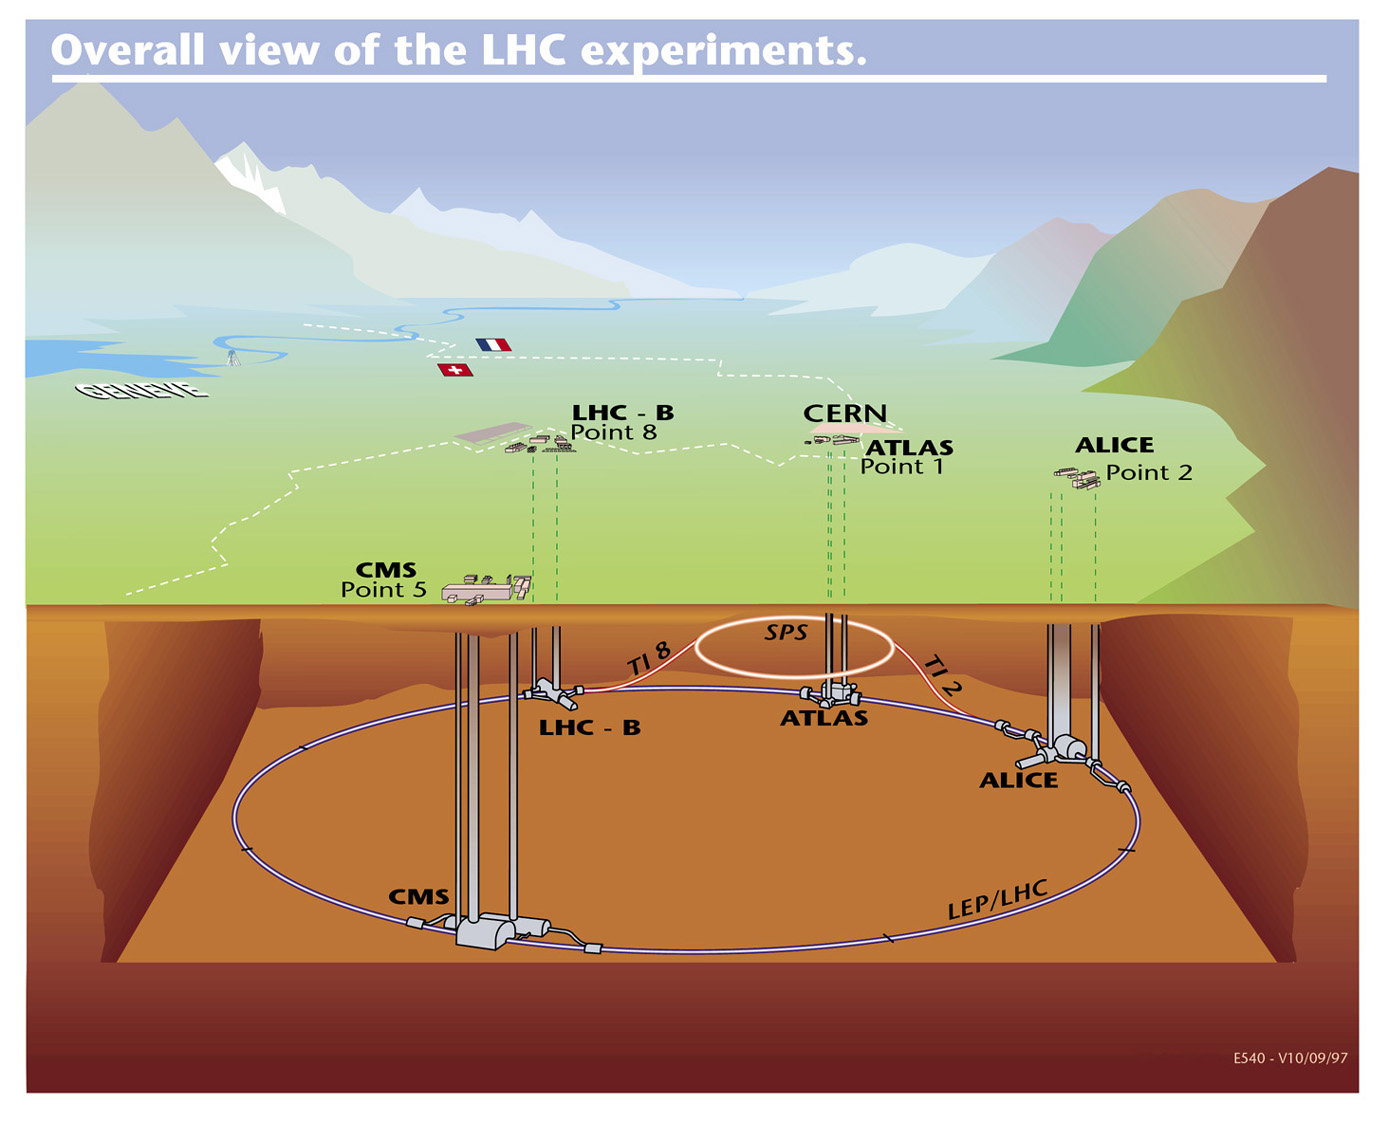
\includegraphics[scale=0.6]{lhc-underground.jpg}
\end{center}
\caption{Vis�o esquem�tica da fronteira franco-su��a mostrando o CERN e os
pontos de accesso aos po�os dos 4 experimentos do LHC.}
\label{fig:aerial}
\end{figure}

O LHC estar� apto a produzir cerca de 40.000.000 milh�es de intera��es por
segundo (ou 40 MHz) e estar� dedicado a cada um dos experimentos de forma
alternada com rela��o a paradas para o enchimento do feixe (do ingl�s
\idxeng{fill}). Cada per�odo de aquisi��o programada ou \idxeng{run} durar�
cerca de 10 horas. Os experimentos ter�o este per�odo para adquirir dados e
perseguir o objetivo f�sico a que se destinam.

\section{O Experimento ATLAS}
\index{ATLAS}

Um dos objetivos principais do experimento ATLAS � descobrir e estudar o
\idx{b�son de Higgs}. Esta part�cula tem import�ncia cr�tica na teoria das
part�culas, como destacado no Cap�tulo~\ref{chap:introducao}, pois est�
diretamente ligada ao conceito de ``massa''\index{conceito de massa} e,
portanto, das part�culas.

\paragraph{A charada da massa} � interessante notar que um conceito t�o
familiar como a massa n�o era entendido at� a proposi��o do \idx{Modelo
Padr�o}. A maioria de n�s est� familiarizado com campos magn�ticos, el�tricos
e gravitacionais. Uma pessoa no campo gravitacional da Terra sente a sua
for�a. Ondas eletromagn�ticas viajam pelo espa�o da mesma forma que ondas
se propagam sobre �gua. Se este balan�o fosse descrito pela Mec�nica Qu�ntica,
a superf�cie da �gua que carrega as ondas seria chamada de ``campo''.

O Modelo Padr�o prop�e que exista um outro campo ainda n�o observado, um campo
que � praticamente indisting��vel do espa�o vazio. Este campo � normalmente
chamado de \idx{campo de Higgs}. Acredita-se que todo o espa�o seja preenchido
com este campo e, interagindo com ele, part�culas adquirem suas
massas. Part�culas que interajam fortemente com o campo s�o pesadas, enquanto
que aquelas que interajam fracamente tornam-se mais leves.

O campo de Higgs tem ao menos uma nova part�cula associada a ele - o b�son de
Higgs. O detetor ATLAS ser� capaz de detetar esta part�cula, se existir,
tornando-se uma das maiores descobertas f�sicas de todos os tempos.

\section{O Detetor ATLAS}

O detetor ATLAS � um aparato em formato cil�ndrico, capaz de registrar os
subprodutos de colis�es pr�ton-antipr�ton a 40 MHz. A
Figura~\ref{fig:atlas-scheme} mostra um esquema do detetor. Repare na parte
inferior � direita, em escala, o tamanho proporcional das pessoas.

\begin{figure}
\begin{center}
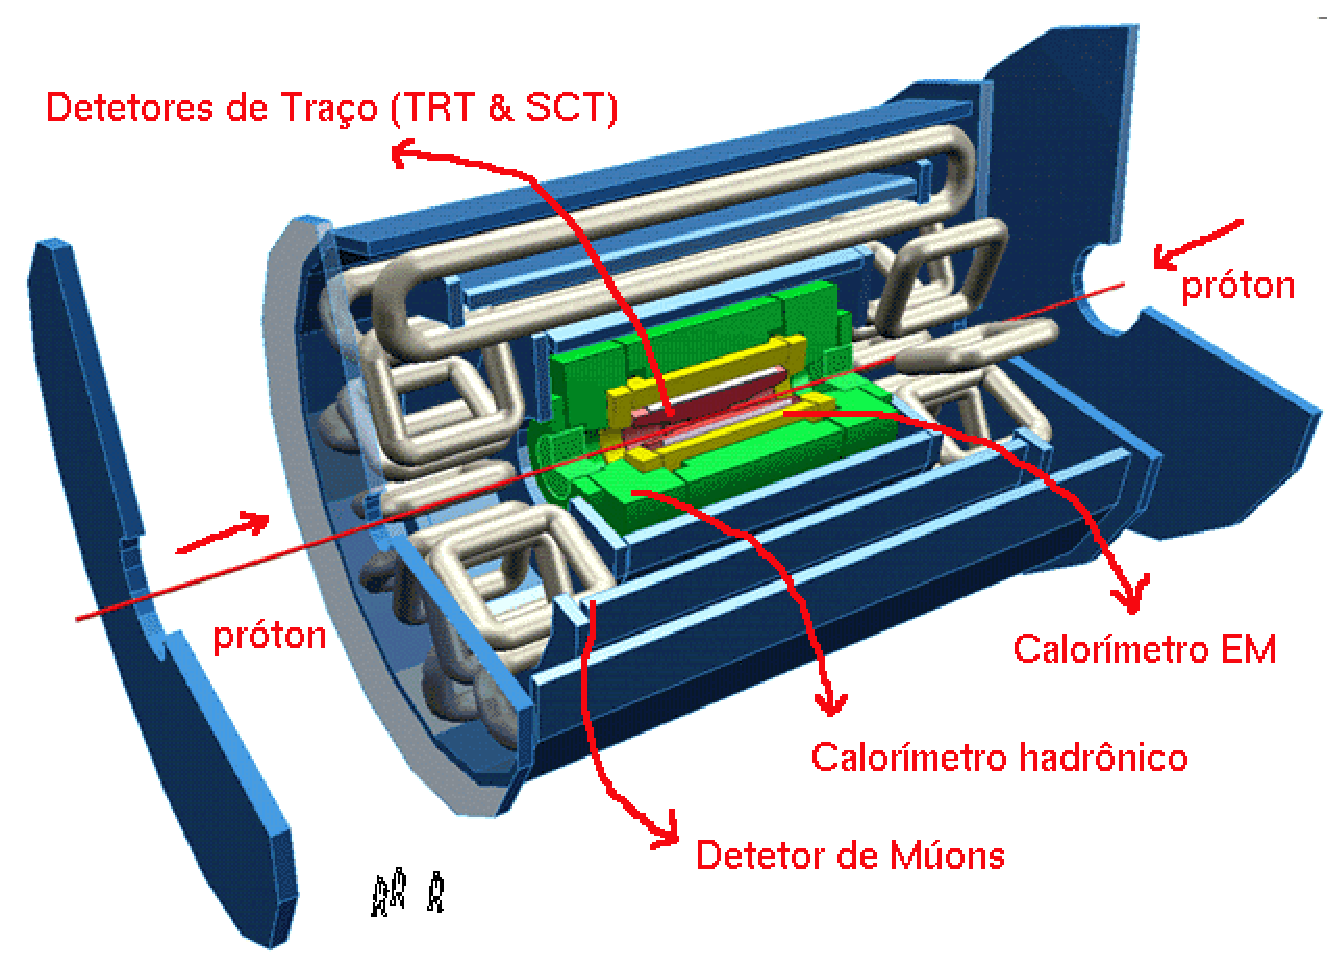
\includegraphics[scale=0.65]{atlas-andre}
\end{center}
\caption{O detetor ATLAS.}
\label{fig:atlas-scheme}
\end{figure}

O detetor \idx{ATLAS} � composto, como mostra a figura, de 4 sistemas de
dete��o independentes. Na parte mais interna, encontram-se detetores de tra�o
altamente segmentados, que podem medir a trajet�ria de part�culas
carregadas. Ao redor deste sistema, ficar� instalado a se��o eletromagn�tica
do calor�metro. Em seguida, vemos a se��o hadr�nica dos calor�metros do ATLAS
e, finalmente, englobando toda a estrutura, detetores de m�ons. A posi��o do
feixe com rela��o ao detetor tamb�m � destacada na figura.

\subsection{Os Detetores de Tra�os}
\index{detetores de tra�os}
\label{sec:atlas-id}

O papel do \idx{Detetor Interno} (do ingl�s \idxeng{Inner Detector}, ID) �
reconstruir tra�os e v�rtices de um evento com alta efici�ncia conjuntamente
ao calor�metro (veja a Se��o~\ref{sec:atlas-calo}) e aos detetores de m�ons
(veja a Se��o~\ref{sec:atlas-muon}), para o reconhecimento de el�trons, f�tons
e m�ons e suprindo assinaturas extras para v�rtices provenientes de part�culas
que decaem rapidamente \cite{atlas-id-tdr}. Sua aceita��o cobre a regi�o de
\idx{pseudo-rapidez} (veja o Ap�ndice~\ref{ap:coord}) de $\pm2,5$, igualando,
em alcance, o restante dos sistemas do detetor ATLAS.

A Figura~\ref{fig:atlas-id-3d} mostra um corte tridimensional do ID. Este
sistema combina detetores de alta resolu��o na parte interna com elementos
para a dete��o de tra�os em modo cont�nuo, na parte externa, todos envolvidos
por um \idx{solen�ide} com campo central de 2 Tesla.

\begin{figure}
\begin{center}
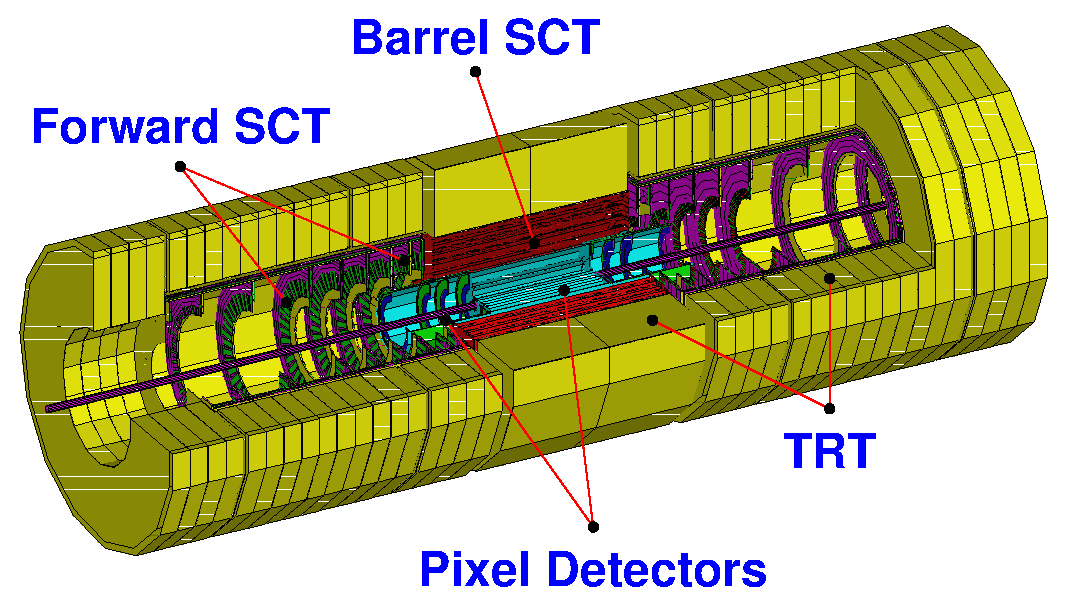
\includegraphics[scale=0.8]{inner_3D}
\end{center}
\caption{Corte tridimensional do Detetor Interno do ATLAS.}
\label{fig:atlas-id-3d}
\end{figure}

Os alvos de momento e resolu��o de v�rtices requerem que medi��es de alta
precis�o sejam feitas com detetores de alta segmenta��o, dada a grande
densidade de tra�os esperada em experimentos ao redor do LHC. \idx{Detetores
de tra�os baseados em semi-condutores} (do ingl�s, \idxeng{Semi-Conductor
Tracker}, \idx{SCT}), usando pastilhas\index{SCT!pastilhas} e
pontos\index{SCT!pontos} (ou \idxeng{pixels}) microsc�picos de sil�cio
oferecem estas caracter�sticas e, portanto, esta tecnologia � utilizada na
parte mais interior do ID. Entretanto, o n�mero total de camadas de precis�o
deve ser limitado por causa do excesso de mat�ria que estes detetores
introduzem e do seu alto custo. Segundo o projeto do ID, a trajet�ria das
part�culas cruzar�, na pior das hip�teses, 4 camadas com sensores em formato
de pastilhas e 3 camadas com sensores em pontos de sil�cio.

Um grande n�mero de pontos da trajet�ria (tipicamente 36 por tra�o) ser�
detetado por um \idx{Detetor de tra�os em microtubos} (do ingl�s,
\idxeng{Straw Tube Tracker}, \idx{TRT}) que prov� a possibilidade do
acompanhamento das trajet�rias em modo cont�nuo com uma quantidade muito menor
de material por ponto e baixo custo. A combina��o destas duas t�cnicas
propicia um reconhecimento de trajet�rias bastante robusto e com alta
precis�o, tanto em $\phi$ como em $z$ (veja a defini��o completa no
Ap�ndice~\ref{ap:coord}. A sensibiliza��o dos microtubos na parte
exterior do detetor contribuir� para a dete��o do momento da part�cula, onde a
baixa precis�o do sistema, se comparado com o SCT, � compensada pelo grande
n�mero de pontos medidos numa maior se��o do espa�o.

\subsection{Os Calor�metros}
\index{calor�metros}
\label{sec:atlas-calo}

Os calor�metros desempenham um papel central na arquitetura do experimento
ATLAS \cite{atlas-calo-tpr}. Estes detetores foram projetados para contribuir
ativamente na filtragem de f�sica interessante e na medi��o precisa de
el�trons, f�tons, jatos e \idx{energia transversa perdida} (do ingl�s
\idxeng{missing $E_{T}$}) no dif�cil ambiente do LHC, trabalhando na sua
m�xima luminosidade.

O sistema pode ser caracterizado funcionalmente ou
arquiteturalmente. Funcionalmente � poss�vel classificar os calor�metros do
ATLAS em:

\begin{itemize}
\item \textbf{Eletromagn�tico ou e.m.}: Para a dete��o de part�culas que
desenvolvem cascatas e.m. como el�trons ou f�tons, situando-se na parte mais
interior da estrutura;

\item \textbf{Hadr�nico}: Para a dete��o de part�culas ou jatos que
desenvolvam cascatas baseadas em h�drons, como n�utrons, pr�tons e p�ons.

\item \textbf{\idx{Avan�ado} ou \idxeng{Forward}}: Para a dete��o de part�culas
pr�ximas ao eixo do feixe de colis�o. Estes dispositivos tendem a ser menos
precisos uma vez que a f�sica envolvida nestes �ngulos de pseudo-rapidez
normalmente n�o representam processos de interesse. Este calor�metro n�o ser�
abordado neste trabalho, em nenhum de seus n�veis, uma vez que � comumente
utilizado somente para efeitos de an�lise \eng{off-line}.
\end{itemize}

Com rela��o � arquitetura dos calor�metros, � poss�vel classificar os
detetores da seguinte forma:

\begin{itemize}
\item \textbf{\idx{Arg�nio L�quido} com \idx{eletrodos de chumbo}}: � um
calor�metro que utiliza o Arg�nio L�quido como material absorvedor e eletrodos
de chumbo para captar os �ons formados durante a intera��o da part�cula com
seu volume. Os eletrodos s�o dispostos em forma de "acorde�o", o que confere a
esta estrutura um formato peculiar. Esta tecnologia foi escolhida para a maior
parte do sistema, cobrindo toda a se��o e.m., as tampas hadr�nicas e para o
calor�metro avan�ado \cite{lar-tdr}.

\item \textbf{\idx{Telhas Cintilantes} ou \idxeng{Tiles}}: � um
calor�metro de amostragem que utiliza uma liga de a�o como material absorvedor
e telhas cintilantes\footnote{Diz-se cintilante o material que emite luz
quando uma part�cula cruza seu volume. A luz emitida � proporcional � energia
da part�cula que passa.} como elemento amostrador. Esta t�cnica foi escolhida
somente para a se��o hadr�nica do barril \cite{tilecal}.
\end{itemize}

A Figura~\ref{fig:calo-general} mostra uma esquematiza��o dos calor�metros do
ATLAS, indicando as partes mencionadas.

\begin{figure}
\begin{center}
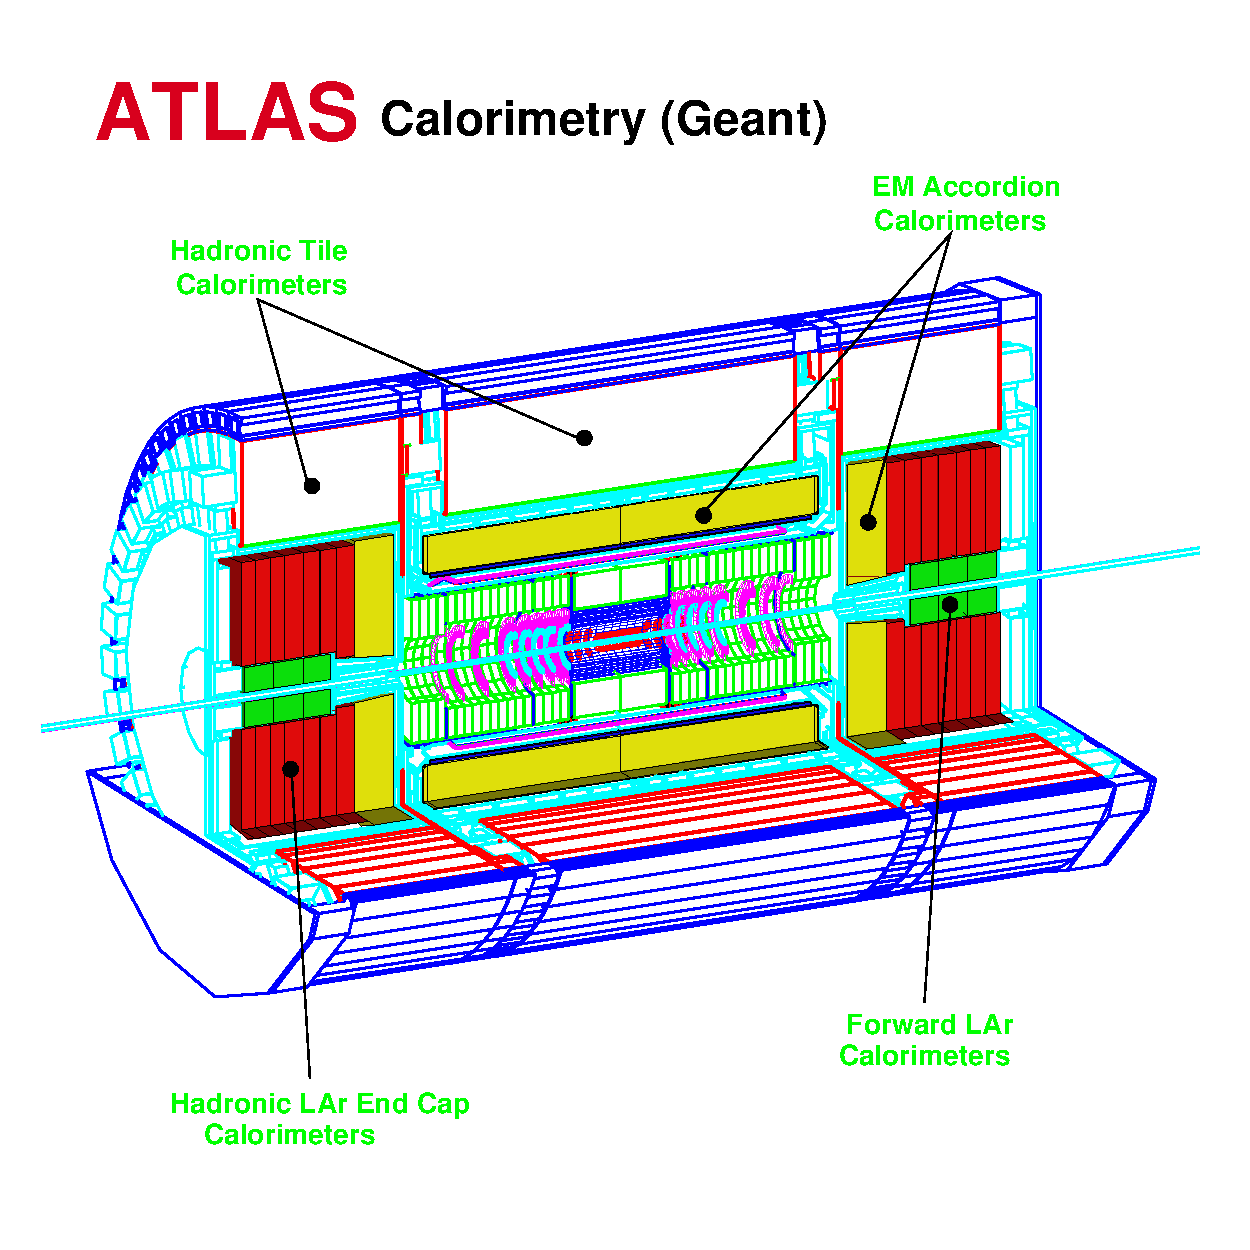
\includegraphics[scale=0.7]{atlas-calorimetry}
\end{center}
\caption{Diagrama esquem�tico dos calor�metros no detetor ATLAS.}
\label{fig:calo-general}
\end{figure}

\subsubsection{A Se��o E.M.}

A se��o e.m. do ATLAS � divida em 3 camadas, das quais a segunda � a mais
profunda. Cada camada possui uma segmenta��o\footnote{A ``segmenta��o"\ de um
detetor � a resolu��o deste no plano $\eta\times\phi$.} espec�fica que otimiza
a rela��o custo-benef�cio do detetor. As camadas mais internas s�o mais
segmentadas, permitindo a localiza��o precisa das part�culas no plano
$\eta\times\phi$, enquanto as mais externas s�o concebidas de forma menos
segmentada e mais profunda, com o objetivo de absorver toda a energia da
part�cula incidente, limitando os custos de produ��o. 

A se��o e.m. � divida em tr�s partes: o barril (do ingl�s
\eng{barrel}) e duas tampas (\eng{endcap}). Estas partes fecham quase que
hermeticamente o espa�o ao redor da colis�o at� um valor de $|\eta|=3,2$ (para
maiores refer�ncias sobre o sistema de coordenadas do ATLAS, leia o
Ap�ndice~\ref{ap:coord}). A Figura~\ref{fig:lar-pos} mostra o posicionamento
do calor�metro eletromagn�tico no detetor ATLAS. Sua segmenta��o n�o �
mostrada nesta figura. Ao inv�s, mostram-se os valores de $\eta$ que definem
os limites geom�tricos da se��o e.m.. Pode-se perceber que a por��o do barril
de tal calor�metro estende-se de $\eta=0$ at� $|\eta|=1,475$. Em
$|\eta|=1,375$, o barril come�a a sobrepor a tampa, que � dividida entre tampa
exterior (at� $|\eta|=2,5$) e interior (de $|\eta|=2,5$ at� $|\eta|=3,2$).

\begin{figure}
\begin{center}
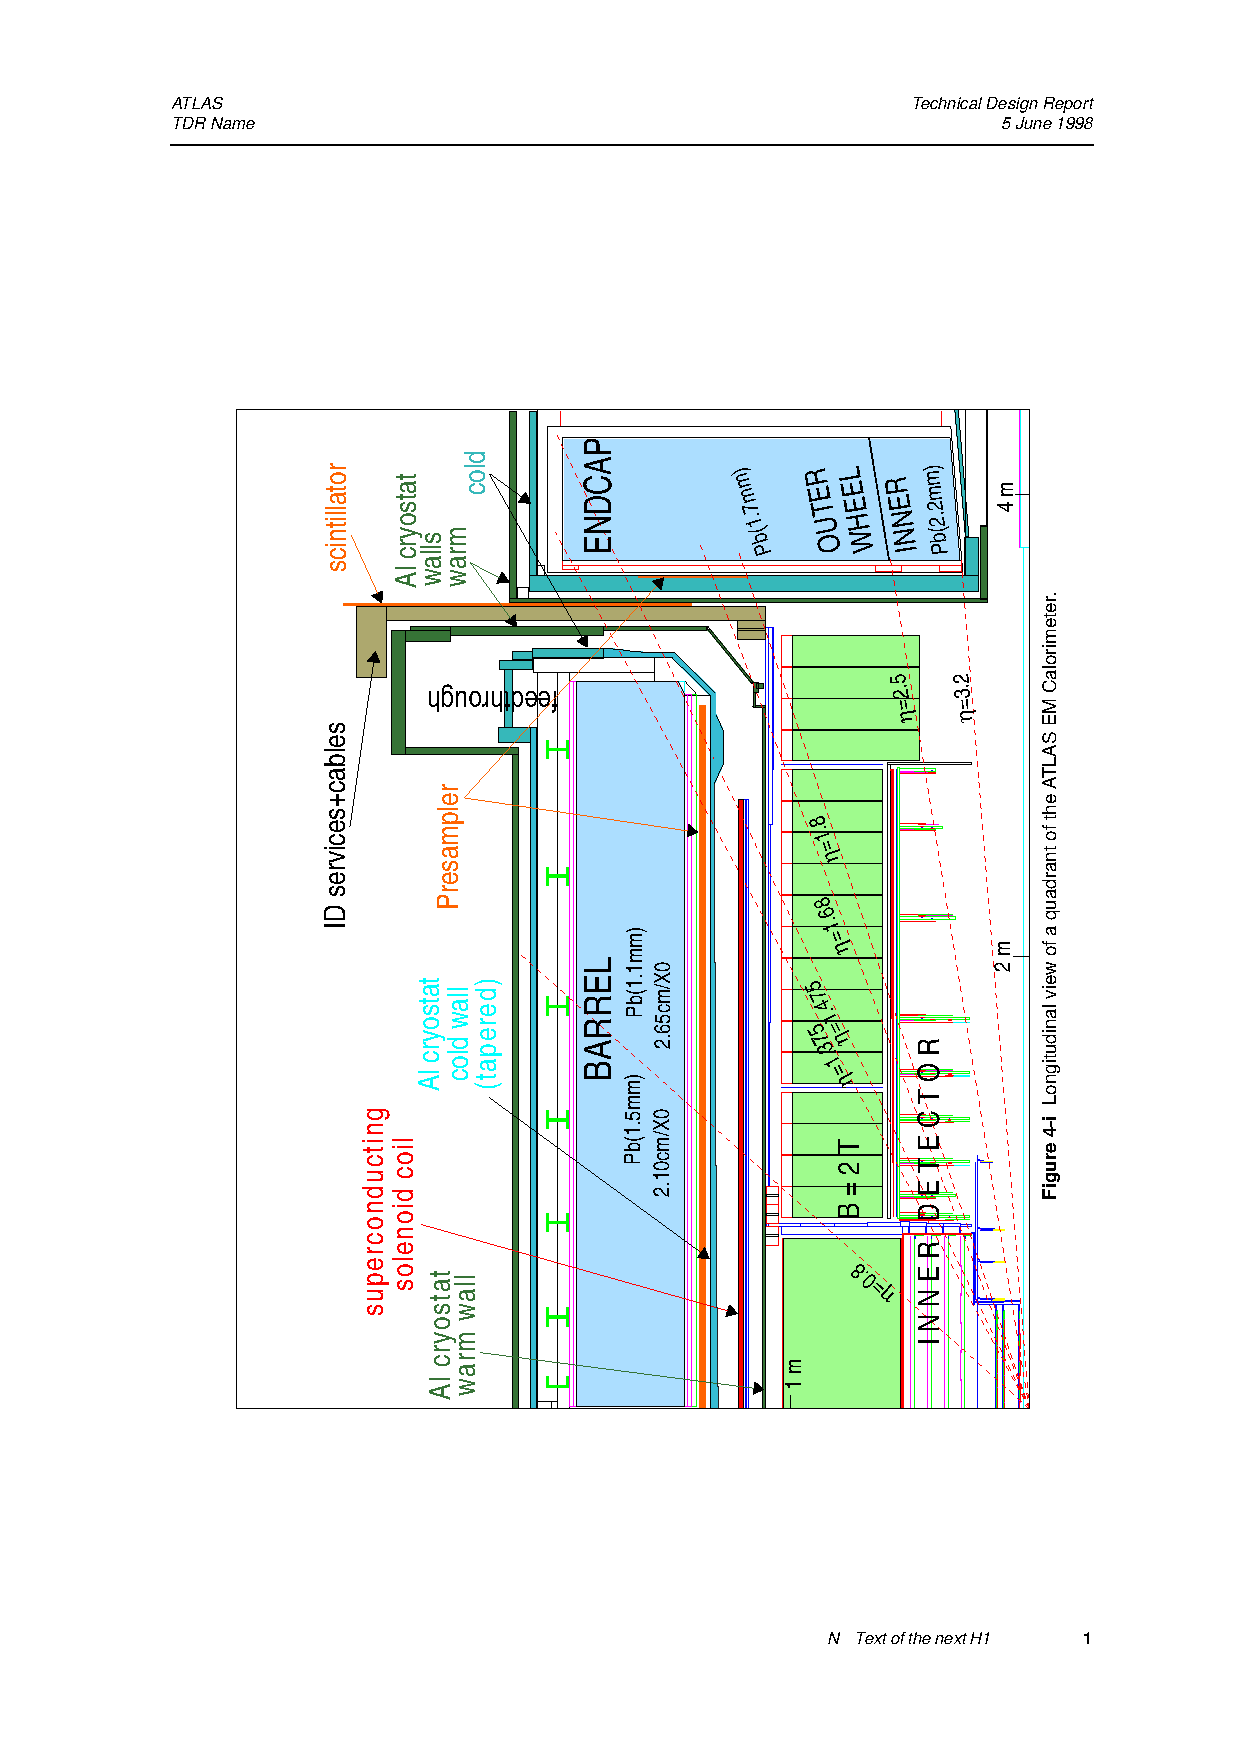
\includegraphics[scale=0.6]{lar-detail}
\end{center}
\caption{O Calor�metro e.m. do ATLAS em um corte transversal.}
\label{fig:lar-pos}
\end{figure}

O calo\-r�\-metro e.m. do ATLAS tam\-b�m inclui um pr�-irradiador (do ingl�s,
\eng{pre-sampler}), que funciona praticamente como um calo\-r�\-metro muito
fino, posicionado antes dos calo\-r�\-metros de ar\-g�\-nio l�\-quido, com a
fun��o de recuperar a informa��o perdida no material \textit{morto} da se��o
e.m. (ou seja, fios, encapamentos, etc.). O pr�-irradiador pode ser observado,
na figura, de $\eta=0$ at� $|\eta|=1,5$ no barril, e depois, de $|\eta|=1,5$
at� $|\eta|=1,8$ nas tampas.

Uma observa��o mais apurada da Figura~\ref{fig:lar-pos} revela um
\textit{buraco} entre o barril e a tampa da se��o e.m.. Esta falha existe para
que seja poss�vel passarem-se os cabos acoplados aos sensores do ID. Para que
a perda nessa regi�o seja minimizada, decidiu-se por colocar um cintilador
(indicado na figura). Cintiladores s�o detetores que se excitam pela passagem
das part�culas energ�ticas e produzem luz. Cintiladores s�o normalmente
bastante compactos e finos.

\paragraph{Segmenta��o da se��o e.m.} O calor�metro e.m. do ATLAS possui
uma segmenta��o constante com rela��o � rota��o (eixo $\phi$), mas vari�vel
com rela��o ao eixo $\eta$. Este calor�metro � dividido em 3 camadas, com
segmenta��es independentes. Isto quer dizer que ao longo do eixo z, a
segmenta��o pode variar. A Figura~\ref{fig:lar-detail} exemplifica a
diversifica��o da segmenta�ao ao longo do eixo $\phi$. Cada camada � formada
por c�lulas de diferentes tamanhos. Nesta figura, tamb�m se verifica que a
segunda camada � a que possui c�lulas mais profundas. � plaus�vel esperar que
mais energia seja amostrada nesta camada.

\begin{figure}
\begin{center}
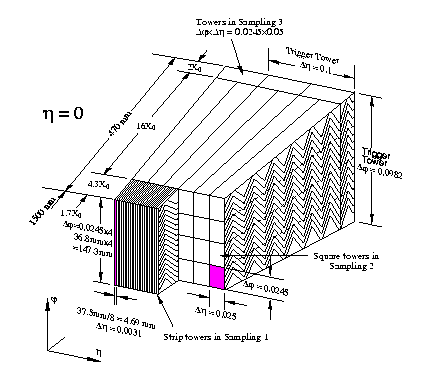
\includegraphics[scale=0.95]{lar-square}
\end{center}
\caption{Diagrama de um dos gomos do barril da se��o e.m. do ATLAS.}
\label{fig:lar-detail}
\end{figure}

A Tabela~\ref{tab:lar} resume as informa��es de segmenta��o para a se��o e.m.,
incluindo informa��es sobre o \eng{pre-sampler} e as tampas. Nota-se, a partir
da tabela, que a segmenta��o de algumas camadas varia bastante com $\eta$. A
coluna da extrema direita indica o n�mero de c�lulas numa �rea de
$0,1\times0,1$ no plano $\eta\times\phi$. Esta �rea � uma refer�ncia para os
n�veis de filtragem, como ser� visto mais adiante.

\begin{table}
\caption{A segmenta��o, camada a camada, dos calo\-r�\-metros e.m. do ATLAS.}
\label{tab:lar}
\index{calor�metro!e.m.!segmenta��o}
\begin{center}
%% Hello emacs, this is -*- latex -*-
\typeout{ ====================================================================}
\typeout{ This is file em-grains.tex, created at 25-Feb-2004 }
\typeout{ Maintained by Andre DOS ANJOS <Andre.dos.Anjos@cern.ch> }
\typeout{ ====================================================================}

\begin{tabular}{||l||l||c||c||c||c||} 
\hhline{|t:=:t:=:t:=:t:=:t:=:t:=:t|}
Camada & Peça & $\eta_{\text{início}}$ & $\eta_{\text{fim}}$& 
$\Delta\eta \times \Delta\phi$& $ N_{\eta} \times N_{\phi} $ \\ 
\hhline{|:=::=::=::=::=::=:|}
\multirow{2}{70pt}{\eng{Pre-sampler}} & Barril & 0 & 1,5 &
	$0,025\times0,1$ & $4 \times 1$\\ 
\hhline{||~||-||-||-||-||-||}
& Tampa & 1,5 & 1,8 & 
	$0,025\times0,1$ & $4 \times 1$ \\ \hhline{|:=::=::=::=::=::=:|}

\multirow{8}{70pt}{Camada 1} & \multirow{2}{40pt}{Barril} & 0& 1,4&
	$0,003125\times1$& $32 \times 1$\\
                  	    & & 1,4 & 1,475 & 
	$0,025\times0,025$& $4 \times 4$ \\
\hhline{||~||-||-||-||-||-||}
& \multirow{6}{70pt}{Tampa} & 1,375& 1,5& $0,025\times0,1$& $1 \times 4$\\
& & 1,5& 1,8& $0,003125\times0,1$& $32 \times 1$\\
& & 1,8& 2,0& $0,004167\times0,1$& $24 \times 1$\\
& & 2,0& 2,4& $0,00625\times0,1$& $16 \times 1$\\
& & 2,4& 2,5& $0,025\times0,1$& $4 \times 1$\\
& & 2,5& 3,2& $0,1\times0,1$& $1 \times 1$\\ \hhline{|:=::=::=::=::=::=:|}

\multirow{4}{70pt}{Camada 2} & \multirow{2}{40pt}{Barril} & 0& 1,4& 
	$0,025\times0,025$& $4 \times 4$\\
		             & & 1,4 & 1,475 & $0,075\times0,025$& $1\times4$\\
\hhline{||~||-||-||-||-||-||}
                             & \multirow{2}{40pt}{Tampa} & 1,375& 2,5& 
	$0,025\times0,025$ & $4 \times 4$\\
			     & & 2,5& 3,2& $0,1\times0,1$ & $1 \times 1$\\
\hhline{|:=::=::=::=::=::=:|}

\multirow{2}{70pt}{Camada 3} & Barril & 0& 1,35& 
$0,05\times0,025$ & $2 \times 4$\\ \hhline{||~||-||-||-||-||-||} 
& Tampa & 1,5 & 2,5& $0,05\times0,025$ & $2 \times 4$\\
\hhline{|b:=:b:=:b:=:b:=:b:=:b:=:b|}

\end{tabular}

\typeout{ *************** End of file em-grains.tex *************** }

\end{center}
\end{table}

\subsubsection{A Se��o Hadr�nica}

Os calor�metros hadr�nicos do ATLAS s�o formados pelo \idx{Calor�metro de
Telhas} ou \idxeng{TileCal} e pela Tampa Hadr�nica baseada em Arg�nio L�quido
- a mesma t�cnica usada para a se��o e.m.. O TileCal � um calor�metro de
amostragem cujo material absorvedor � uma liga com a�o e os elementos
amostradores s�o telhas cintilantes \cite{tilecal}. As telhas s�o posicionadas
em planos perpendiculares aos feixes de part�culas colididas e conectadas a
fibras �pticas em duas de suas extremidades. Estas fibras coletam o sinal
luminoso, gerado pela telha ao interagir com a part�cula, e transportam-no at�
tubos fotomultiplicadores (PM)\index{tubos fotomultiplicadores}, onde o sinal
� convertido em sinal el�trico. Somadores r�pidos \cite{seixas:adder} se
encarregam de adicionar os sinais das telhas entre si formando c�lulas de
dete��o, de forma equivalente � se��o e.m.. O TileCal � posicionado ap�s a
se��o e.m., como � poss�vel verificar na Figura~\ref{fig:tile-pos}.

\begin{figure}
\begin{center}
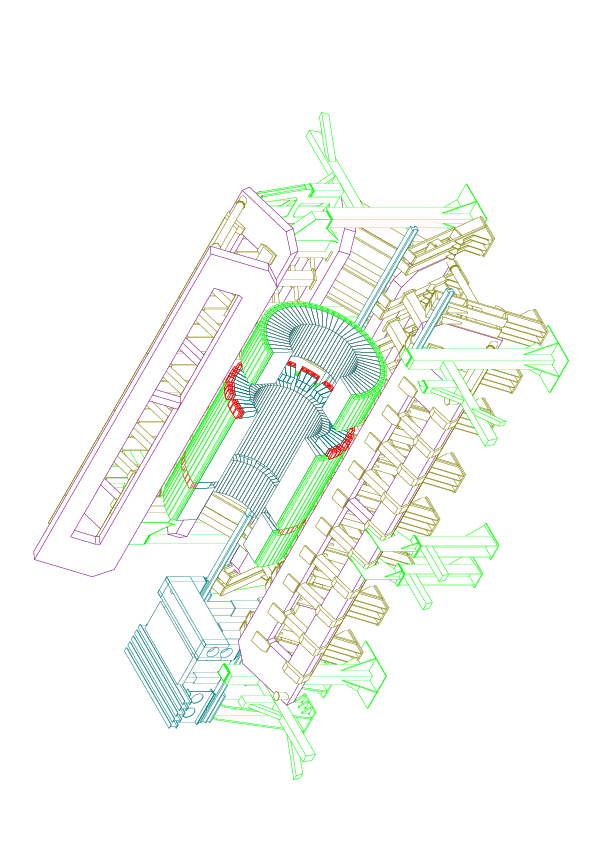
\includegraphics[scale=0.5,angle=-90]{tilecal-3d}
\end{center}
\caption{O calor�metro de telhas do ATLAS (em verde ao centro), em sua posi��o
final, envolvido pelo detetor de m�ons (em roxo e marrom).}
\label{fig:tile-pos}
\end{figure}

Uma peculiaridade dos calor�metros hadr�nicos do ATLAS � que o barril e a
tampa s�o feitos de formas diferentes, ao contr�rio da se��o e.m.. O
calor�metro de telhas (TileCal) abrange as por��es do barril ($0<|\eta|<1,0$)
e sua extens�o ($0,8<|\eta|<1,7$). A tampa desta se��o � feita como os
calor�metros e.m., no formato de acorde�es, usando Arg�nio l�quido.

A Tabela~\ref{tab:had} resume a informa��o de segmenta��o da se��o hadr�nica
dos calor�metros do ATLAS, de forma equivalente a da Tabela~\ref{tab:lar}.
Nessa tabela � poss�vel perceber que o tamanho das c�lulas, em m�dia, � bem
maior que o valor equivalente no calor�metro eletromagn�tico. A segmenta��o
� tamb�m mais uniforme que na se��o e.m. dos calor�metros do ATLAS. Isto se
deve ao fato dos chuveiros hadr�nicos serem mais largos e profundos,
provocando maiores flutua��es nas medidas de energia e, portanto, n�o
necessitando de uma segmenta��o t�o fina.

Outra diferen�a � na �rea de refer�ncia. Na se��o e.m., considera-se
$0,1\times0,1$ - aqui a �rea de refer�ncia � de $0,2\times0,2$, j� que se
encontram c�lulas maiores que a �rea de refer�ncia no calor�metro e.m..

\begin{table}
\caption{A segmenta��o, camada a camada, dos calo\-r�\-metros ha\-dr�\-nicos
do ATLAS.}
\label{tab:had}
\index{calor�metro!hadr�nico!segmenta��o}
\begin{center}
%% Hello emacs, this is -*- latex -*-
\typeout{ ====================================================================}
\typeout{ This is file had-grains.tex, created at 25-Feb-2004 }
\typeout{ Maintained by Andre DOS ANJOS <Andre.dos.Anjos@cern.ch> }
\typeout{ ====================================================================}

\begin{tabular}{||l||l||c||c||c||c||} 
\hhline{|t:=:t:=:t:=:t:=:t:=:t:=:t|}
Camada& Pe�a & $\eta_{\text{in�cio}}$ & $\eta_{\text{fim}}$& 
$\Delta\eta \times \Delta\phi$& $ N_{\eta} \times N_{\phi} $ \\ 
\hhline{|:=::=::=::=::=::=:|}
\multirow{4}{50pt}{Camadas 1 e 2} & Barril (TileCal)& 0 & 1,0 & 
	$0,1\times0,1$ & $2\times2$ \\
\hhline{||~||-||-||-||-||-||}
				  & Barril Ext. (TileCal)& 0,8 & 1,7 & 
	$0,1\times0,1$ & $2\times2$ \\
\hhline{||~||-||-||-||-||-||}
	& \multirow{2}{60pt}{Tampa (LAr)} & 1,5 & 2,5 &
	$0,1\times0,1$ & $2\times2$ \\
	&                           & 2,5 & 3,2 & 
	$0,2\times0,2$ & $1\times1$ \\

\hhline{|:=::=::=::=::=::=:|}

\multirow{4}{50pt}{Camada 3} & Barril (TileCal)& 0 & 1,0 & 
	$0,2\times0,1$ & $1\times2$ \\
\hhline{||~||-||-||-||-||-||}
				  & Barril Ext. (TileCal)& 0,8 & 1,7 & 
	$0,2\times0,1$ & $1\times2$ \\
\hhline{||~||-||-||-||-||-||}
	& \multirow{2}{60pt}{Tampa (LAr)} & 1,5 & 2,5 & 
	$0,1\times0,1$ & $2\times2$ \\
	&                           & 2,5 & 3,2 & 
	$0,2\times0,2$ & $1\times1$ \\

\hhline{|b:=:b:=:b:=:b:=:b:=:b:=:b|}

\end{tabular}

\typeout{ *************** End of file had-grains.tex *************** }

\end{center}
\end{table}

A Figura~\ref{fig:tilecell} mostra uma se��o transversal da parte do Barril do
Calor�metro de Telhas. Nesta figura, verifica-se que o sistema de leitura
agrupa as c�lulas deste detetor em 3 camadas. A segmenta��o no sentido de
$\eta$ � mantida constante ainda assim.

\begin{figure}
\begin{center}
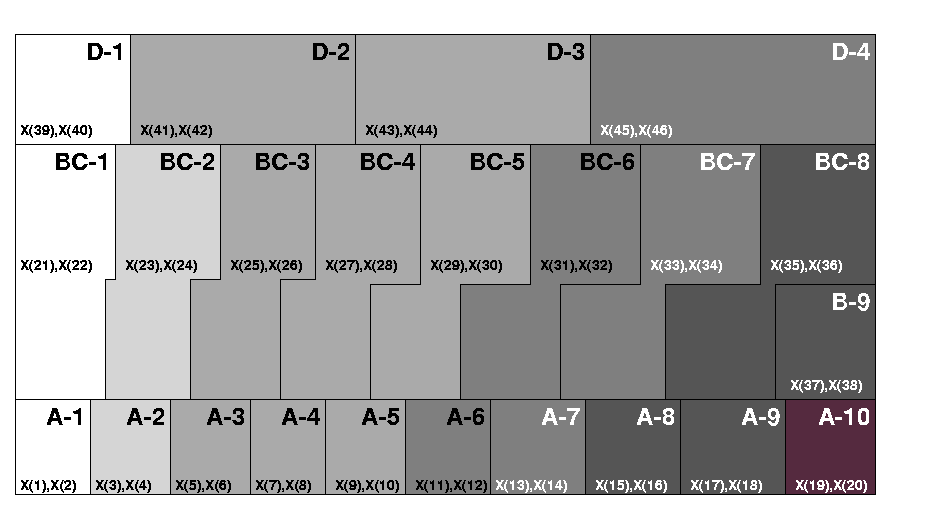
\includegraphics[scale=0.5]{tilecell}
\end{center}
\caption{Configura��o de leitura das c�lulas da se��o do barril do Calor�metro
de Telhas.}
\label{fig:tilecell}
\end{figure}

\subsection{O Detetor de M�ons}
\index{detetor de m�ons}
\label{sec:atlas-muon}

\idx{M�ons} com grande momento s�o \idx{assinaturas} bastante
promissoras e robustas da f�sica de interesse no LHC. Para explorar este
potencial, foi projetado um spectr�metro de m�ons (veja a
Figura~\ref{fig:atlas-muon-3d}) com sistemas de filtragem e medi��o de momento
com alta resolu��o independentes do restante do sistema, sens�vel a este tipo
de part�culas \cite{atlas-mu-tdr}. A dete��o � baseada na deflex�o (magn�tica)
de m�ons provida por um grande tor�ide com n�cleo a ar e detetores de tra�o
bastante precisos. Para $|\eta| \leq 1,0$, um grande magneto em formato de
barril ser� constru�do com oito molas circundando a se��o hadr�nica dos
calor�metros. Para $1,4 \leq |\eta| \leq 2,7$, a deflex�o ser� garantida por
magnetos na forma de tampas ao redor do barril. Esta configura��o prov� um
campo magn�tico praticamente transversal � trajet�ria de eventuais m�ons.

\begin{figure}
\begin{center}
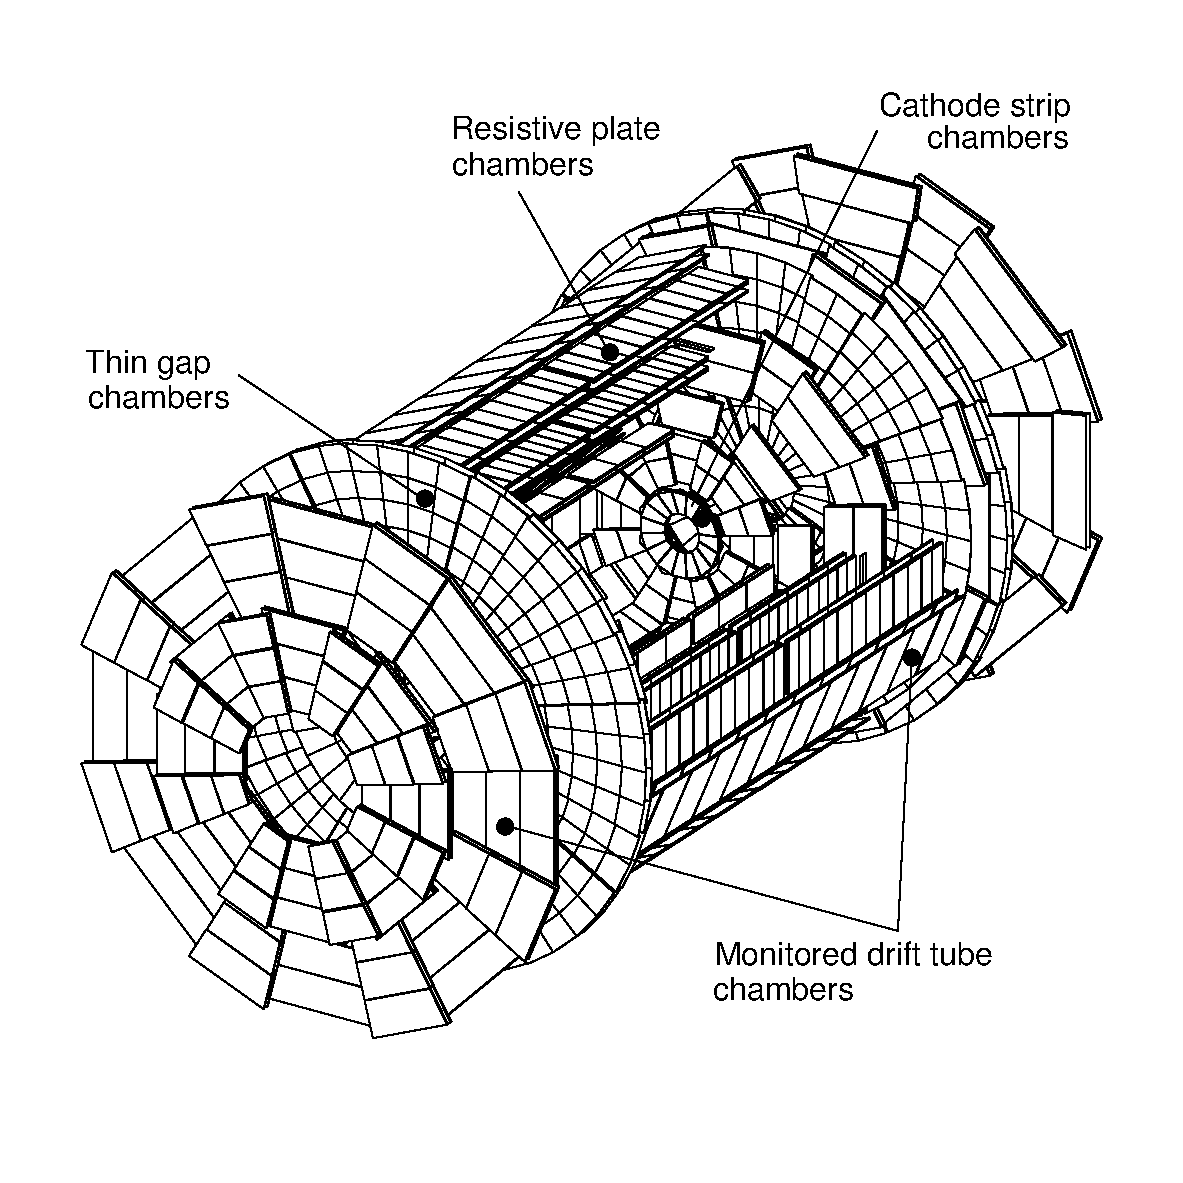
\includegraphics[scale=0.7]{muon-detector}
\end{center}
\caption{Vis�o tridimensional dos detetores de m�ons do ATLAS.}
\label{fig:atlas-muon-3d}
\end{figure}

Na regi�o do barril, as trajet�rias ser�o detetadas por c�meras organizadas em
tr�s camadas cil�ndricas (esta��es) ao redor do eixo de colis�o. Na regi�o da
tampa, as c�maras ser�o montadas verticalmente, tamb�m em n�mero de tr�s. As
coordenadas dos tra�os � medida precisamente por \idx{C�maras de Tra�os
Monitoradas} (do ingl�s, \idxeng{Monitored Drift Chambers}, MDT) na dire��o
principal de deflex�o do campo magn�tico, na maior parte do campo da
pseudo-rapidez. Para grandes valores de pseudo-rapidez, \idx{C�maras de
Pastilhas Cat�dicas} (do ingl�s, \idxeng{Cathode Strip Chambers}, CSC) com
alta segmenta��o ser�o constru�das para garantir a precis�o da dete��o nesta
�rea bastante ruidosa. Tal como os calor�metros, o Spectr�metro de M�ons est�
diretamente acoplado ao primeiro n�vel do sistema de filtragem de eventos do
ATLAS (Veja o Cap�tulo~\ref{chap:trigger}).

\typeout{ *************** End of file atlas.tex *************** }

%% Hello emacs, this is -*- latex -*-
\typeout{ ====================================================================}
\typeout{ This is file trigger.tex, created at 28-Feb-2004 }
\typeout{ Maintained by Andre dos Anjos <Andre.dos.Anjos@cern.ch> }
\typeout{ ====================================================================}

\chapter{O Sistema de Filtragem e Aquisição de dados do ATLAS}
\label{chap:trigger}

O \idx{sistema de filtragem} do experimento ATLAS tem o encargo de separar, de
forma \eng{online}, a Física considerada como ordinária segundo o experimento,
dos raros eventos de interesse. A taxa de eventos produzida pelo LHC será de
40 milhões por segundo, ou 40 MHz, em bateladas que durarão cerca de 10 horas
(este período é comumente referido como \eng{run}). Cada evento poderá
produzir uma colisão favorável à Física de interesse, embora a grande maioria,
mais de 99,9999\%, represente canais físicos já bastante estudados em
experimentos anteriores, ainda que a luminosidade do sistema seja tão
elevada. Ademais, cada evento detetado pelo ATLAS produzirá cerca de 1,5
Megabytes em dados, o que torna o problema da filtragem bastante difícil, já
que o fluxo de dados que deve ser analisado por base de tempo está acima da
capacidade de qualquer tecnologia de transporte de dados atual.

Para o experimento ATLAS, o sistema de filtragem será construído em 3 níveis
seqüenciais (veja a Figura~\ref{fig:trigger-sketch}). Cada nível que se sucede
refina a decisão do nível anterior através da aquisição de mais dados do
detetor. O \idx{Primeiro Nível} de filtragem (do inglês \idxeng{First-Level
Trigger}, LVL1) deverá reduzir a taxa de eventos do LHC para cerca de 100 kHz
apenas, através de técnicas simples de filtragem codificadas em hardware
dedicado. O \idx{Segundo Nível} de filtragem (do inglês
\idxeng{Second-Level Trigger}, LVL2) reduzirá a taxa de saída do LVL1 para
aproximadamente 1 kHz utlizando aplicações codificadas em software para
computadores do tipo PC, tão comuns quanto os disponíveis para aplicações
domésticas. O \idx{Terceiro Nível} de filtragem ou
\idx{Filtro de Eventos} (do inglês \idxeng{Event Filter}, EF) estará baseado
na mesma tecnologia escolhida para o LVL2, reduzindo a taxa de entrada de
eventos para aproximadamente 100 Hz, através de algoritmos de filtragem mais
eficientes porém com menor desempenho. Os eventos ultimamente selecionados
pelo EF são armazenados em mídia permanente, para posterior análise
\eng{offline}. 

\begin{figure}
\begin{center}
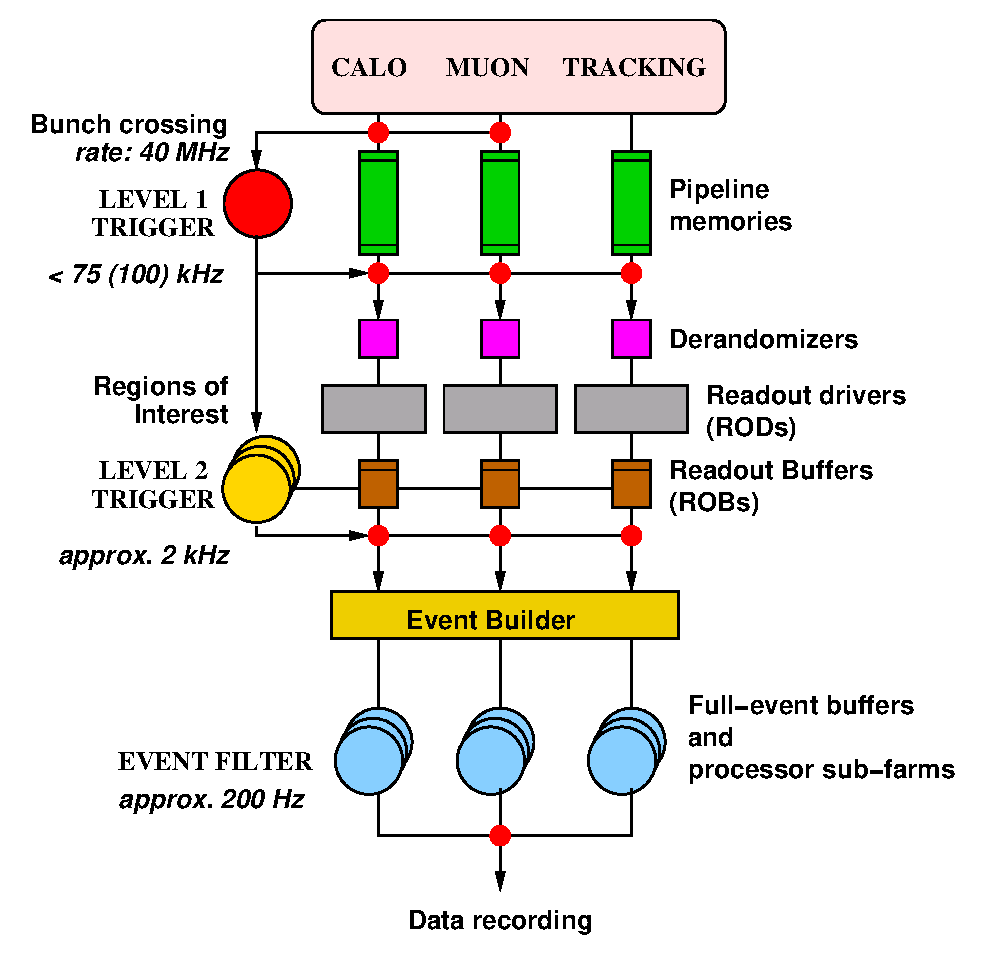
\includegraphics[angle=-90,scale=0.8]{trigger-sketch}
\end{center}
\caption[Visão funcional simplificada do sistema de filtragem do experimento
ATLAS.]{Visão funcional simplificada do sistema de filtragem do experimento
ATLAS. Extraído de \cite{hlt-tdr}.}
\label{fig:trigger-sketch}
\end{figure}

\section{O Primeiro Nível de Filtragem}
\label{sec:lvl1}

O Primeiro Nível de Filtragem (LVL1) realiza uma seleção inicial de candidatos
à Física de interesse baseada em informações com segmentação reduzida,
fornecidas por um subconjunto dos detetores do ATLAS, os calorímetros e os
detetores de múons \cite{l1-tdr}. Múons com altos valores de \idx{momento
transverso} ($p_T$) são identificados a partir das câmaras de trigger
conectadas ao Spectrômetro de Múons (veja a Seção~\ref{sec:atlas-muon}) na
região do barril e da tampa. As seleções baseadas em calorimetria utilizam uma
segmentação reduzida das seções e.m. e hadrônica no barril e na tampa. Os
objetos procurados usando-se calorímetros no LVL1 são elétrons com altos
valores de $p_T$ e fótons, jatos, taus decaindo em cascatas hadrônicas,
grandes quantidades de energia faltante ou energia transversa total. No caso
da seleção de elétrons e fótons ou hádrons e taus, isolamento em
energia\footnote{Isolamento em energia significa a ausência de outros picos
energéticos adjacentes ao pico energético sendo analisado.} pode ser
requisitado.

Para gerar os sinais de filtragem necessários ao LVL1, o sistema de leitura de
dados dos calorímetros é equipado com somadores rápidos \cite{seixas:adder,
lar-tdr} que aglomeram o sinal de 2 ou mais células destes detetores para
gerar macrocélulas de filtragem denominadas \idx{torres de filtragem} (do
inglês \idxeng{Trigger Towers}, TT). O sistema de múons também possui
circuitos equivalentes que determinam a ocorrência de traços com altos valores
de $p_T$ naquele subdetetor.

Os eventos selecionados pelo LVL1 são lidos a partir da eletrônica específica
de cada dos detetor por meio de \eng{drivers} denominados \idxeng{ReadOut
Drivers} ou \idx{ROD}'s. Cerca de 1.600 ROD's serão necessários para ler todos
os dados do detetor, ou seja, aproximadamente $10^7$ canais
independentes. Vários canais de leitura são multiplexados em cada ROD. Bancos
de memória primários, chamados de \idxeng{derandomizers}, garantem um fluxo
contínuo dos dados aos ROD's, apesar da irregularidade da aceitação de eventos
proporcionada pelo LVL1.

Os dados completos de eventos selecionados são guardados momentaneamente em
bancos de memória denominados \idxeng{ReadOut Buffers} (ROB's) até que o
evento seja rejeitado pelo LVL2 ou, no caso de ser aceito por este nível, até
que os dados sejam transferidos para o terceiro nível de filtragem (EF). O
processo de mover os dados dos ROB's para o EF é chamado de \idx{construção do
evento} (do inglês, \idxeng{Event Building}, EB). Porém, até a fase de
construção do evento, os dados estarão segmentados em ROB's. Após esta etapa,
o evento completo estará guardado em um único banco de memória e acessível a
um processador do EF.

\paragraph{Regiões de Interesse} Além do disparo dado pelo LVL1 à eletrônica de
leitura, este nível de filtragem deve enviar ao LVL2 um mapa dos objetos de
interesse encontrados no detetor durante a avaliação do evento. Este mapa
indica, na precisão do LVL1, as \idx{regiões de interesse} no detetor (do inglês
\idxeng{Region of Interest}, RoI) que contribuíram para a seleção, os tipos
de objetos encontrados e o valor mínimo (\eng{threshold}) de $p_T$ que
satisfazem. Informações de RoI's secundárias (que não contribuíram para a
decisão do LVL1, mas que excitaram notavelmente o detetor) também podem ser
transmitidas ao LVL2, provendo maior flexibilidade de decisão a este nível.

Na Figura~\ref{fig:l1-context}, é possível observar um diagrama do tipo
``caixa-preta'', indicando os sinais de entrada e saída do LVL1. A este
sistema são injetados os sinais provenientes da eletrônica de leitura e dos
sistemas de filtragem diretamente acoplados aos detetores e do LHC
(\eng{clock} de 40 MHz). Deste sistema serão colhidos sinais que serão, por
sua vez, encaminhados para o LVL2, para a eletrônica de aquisição e para o
sistema de monitoração central.

\begin{figure}
\begin{center}
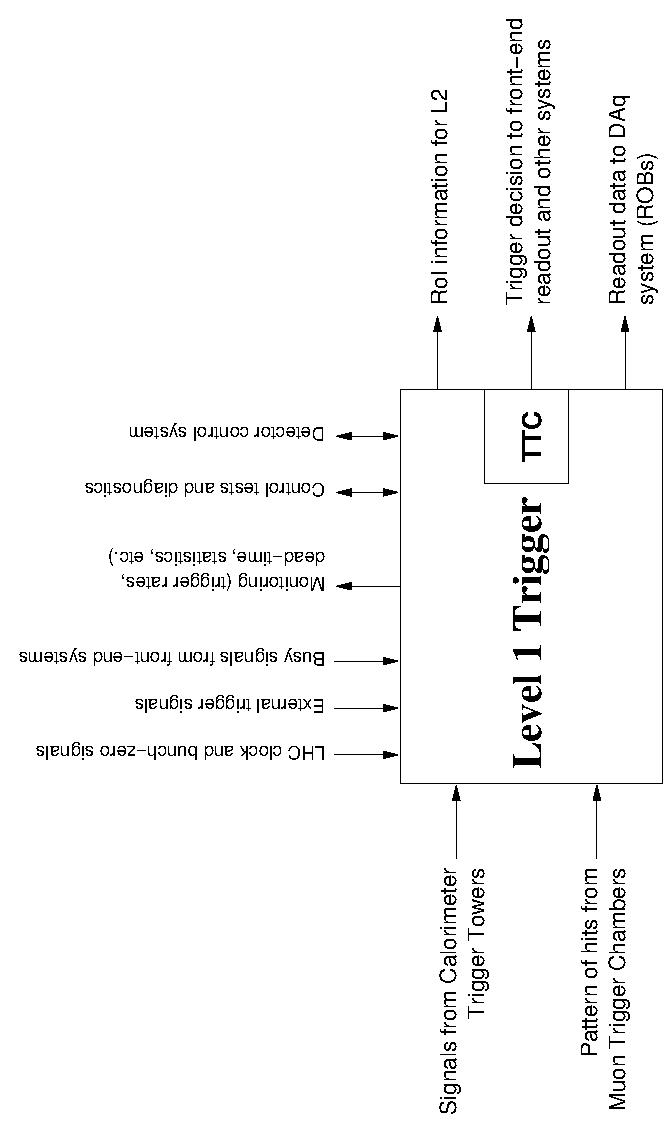
\includegraphics[scale=0.75,angle=-90]{l1-blackbox}
\end{center}
\caption[Diagrama simplificado dos sinais de entrada e saída do
LVL1.]{Diagrama simplificado dos sinais de entrada e saída do LVL1. Extraído
de \cite{hlt-tdr}.}
\label{fig:l1-context}
\end{figure}

Na Figura~\ref{fig:l1-functional} observa-se um diagrama funcional
simplificado do LVL1. Nesta figura é possível identificar processadores
específicos para os sinais provenientes dos detetores. Um \idx{processador
central de filtragem} (marcado na figura como \idxeng{Central Trigger
Processor}) é responsável pela decisão final e pela emissão do sinal para o
LVL2 e para o sistema de distribuição de tempo, disparo e controle (indicado
como \idxeng{Timming, Trigger and Control distribution}, ou TTC), que gera,
finalmente, o sinal para a leitura dos dados do detetor. Dentre os componentes
do TTC está o \idx{Construtor de RoI's} (do inglês \idxeng{RoI Builder}, RoIB)
que monta o mapa de RoI's destacadas pelo LVL1 e comunica, através de uma
conexão serial rápida tipo S-Link, estes dados ao LVL2.

\begin{figure}
\begin{center}
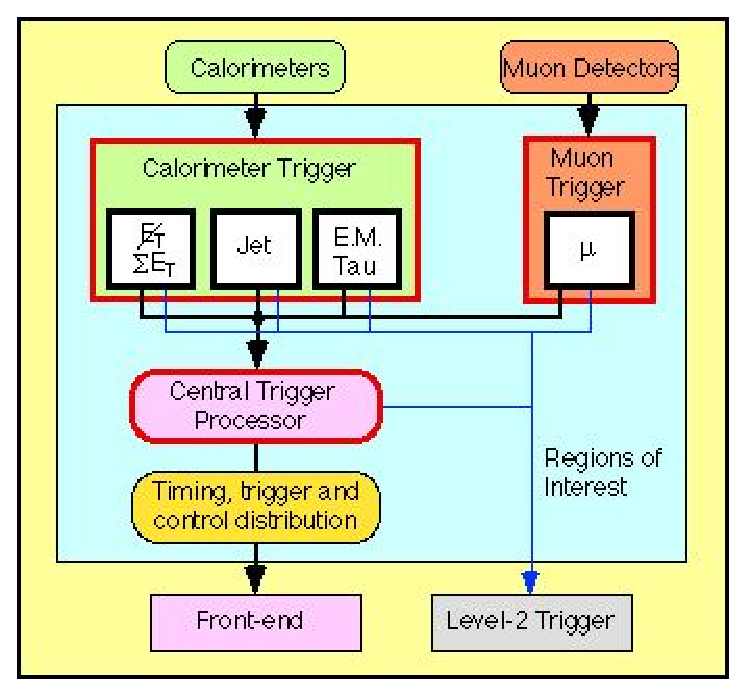
\includegraphics[scale=0.8]{l1-functional}
\end{center}
\caption[Diagrama em blocos indicando as principais funções do LVL1.]{Diagrama
em blocos indicando as principais funções do LVL1. Extraído de \cite{hlt-tdr}.}
\label{fig:l1-functional}
\end{figure}

\section{Os Altos Níveis de Filtragem, Aquisição de Dados e Controle}
\label{sec:hlt-daq}

%% Observação: falta referência para S-Links

O \idx{sistema de aquisição de dados} do ATLAS (do inglês \idxeng{Data
Acquisition System}, \idx{DAQ}) é composto por processadores que estão
encarregados da transmissão e manipulação dos dados produzidos pelo detetor
\cite{hlt-tdr}. O DAQ trabalha em cooperação com os diversos níveis de
filtragem e controle do experimento de forma a garantir a correção dos dados
transmitidos e a minimização do tempo morto despendido no tráfego de
informação pelo sistema. A cadeia de operação do DAQ é iniciada por um disparo
do LVL1 para a leitura de dados executada nos ROD's. Cada ROD é ligado,
através de uma conexão S-Link\footnote{Conexão ponto-a-ponto com taxa máxima
de transferência de 160 megabits por segundo.}, a somente um ROB. Cada ROB
pode receber dados de um ou no máximo 3 ROD's, dependendo da configuração
final do experimento.

Cabe aos \idx{Altos Níveis de Filtragem} (do inglês \idxeng{High-Level
Triggers}, \idx{HLT}), analisando de forma ótima os dados presentes nos ROB's,
decidir, disparando mais uma vez o DAQ, sobre o futuro de cada evento aceito
pelo LVL1. O conjunto HLT-DAQ-Controle deverá funcionar harmoniosamente sobre
uma mesma base computacional, utilizando ainda o mesmo conjunto de ferramentas
para a codificação, análise e depuração de eventuais problemas que possam
ocorrer. Por esta razão, esta união de produtos de \eng{hardware} e
\eng{software} é considerada um macro-sistema do experimento. Este sistema
pode ser subdividido em 4 partes:

\begin{itemize}
\item \textbf{\idx{Sistema de controle do detetor} ou \idxeng{Detector Control
System}, \idx{DCS}}: responsável pela operação coerente e segura (no que tange
radiação, controle de altas tensões, etc.) do detetor ATLAS e pelo
interfaceamento com sistemas externos e serviços incluindo o acelerador
LHC. Uma vez que este tópico não está diretamente envolvido neste trabalho,
será abordado somente em caráter introdutório;

\item \textbf{\idxeng{Online}}: é responsável por todos os aspectos de
operação e controle durante a aquisição de dados do experimento e durante
\eng{runs} de teste e calibração;

\item \textbf{\idx{Fluxo de dados} ou \idxeng{Dataflow}}: este sistema é
responsável por receber os dados do detetor, servir um subconjunto destes
dados ao HLT e transportar os dados de eventos selecionados em última
instância para armazenagem em mídia permanente;

\item \textbf{\idx{Altos Níves de Filtragem} ou \idx{HLT}}: são responsáveis pela
seleção de eventos após o LVL1, envolvendo a redução da taxa de eventos e a
classificação de todos os eventos aceitos.

\end{itemize}

\subsection{O Sistema de Controle do Detetor}
\label{sec:dcs}

O DCS supervisa todos os componentes de \eng{hardware} do arranjo
experimental, incluindo todos os sistemas de deteção do ATLAS e a
infraestrutura experimental comum a todos os outros sistemas. O DCS também se
comunica com sistemas externos, como a infraestrutura de serviços do CERN e,
mais notavelmente, com o acelerador LHC.

Aspectos de seguranção são tratados pelo DCS somente no nível de menor
severidade. Este trabalho tange principalmente questões ligadas ao
seqüenciamento de operações ou à requisição onde prevaleçam condições
específicas, antes de permitir que outros procedimentos sejam
executados. Ferramentas para a construção de interdependências, tanto em
\eng{hardware} quanto em \eng{software}, são providas pelo DCS. Monitoração e
prevenção de situações que poderiam causar danos maiores ao detetor e à vida
das pessoas são de responsabilidade de sistemas dedicados - o \idx{Sistema de
Segurança do Detetor} (do inglês \idxeng{Detetor Safety System}, \idx{DSS}) e
do sistema de segurança e alarme do CERN respectivamente. O DCS interage com
ambos os sistemas.

Todas as ações iniciadas pelo operador e todos os erros, avisos e alarmes que
impliquem em falha de \eng{hardware} do detetor são gerenciadas pelo DCS. Este
sistema provê informação \eng{online} da situação presente, com a
granularidade necessária para uma operação centralizada do sistema. A
interação dos \eng{experts} em detetores com suas máquinas também é feita
através do DCS, que continuamente monitora todos os parâmetros operacionais,
guiando o operador e sinalizando qualquer comportamento anormal do
maquinário. O DCS também será capaz de acionar procedimentos automáticos para
trazer o sistema de deteção para um estado seguro, se necessário for.

No que tange à operação do experimento, a interação com o sistema de aquisição
de dados é de importância primária. A boa qualidade da Física gravada em mídia
permanente depende de uma sincronização absoluta entre o DAQ e o DCS; ambos os
sistemas são complementares. O DAQ lida com eventos caracterizados por números
e o DCS guarda o estado operacional do detetor enquanto os dados estão sendo
adquiridos, correlacionando os números dos eventos com a qualidade da
aquisição, que, finalmente, é avaliada \eng{offline}.

Algumas partes do detetor operarão continuamente, pois qualquer interrupção
pode ser custosa em tempo, fundos ou desempenho do sistema global. Portanto, a
supervisão do sistema de deteção é necessária constantemente. Por outro lado,
o DAQ é somente necessário durante a aquisição de dados ou durante \eng{runs}
de monitoração, calibração ou teste. Assim sendo, o DCS precisa ter completa
independência funcional, ainda que, ao mesmo tempo, este quesito não deva
imperativamente acarretar em limites operacionais com o DAQ.

\subsection{O Sistema \textit{Online}}
\label{sec:online}

O sistema \idxeng{online} engloba o conjunto de aplicações para configurar,
controlar e monitorar o sistema de filtragem e aquisição de dados do ATLAS (do
inglês \eng{Trigger and Data Acquisition}, TDAQ), excluindo o gerenciamento,
processamento e transporte de dados físicos. É um conjunto personalizável de
ferramentas que provê a ``cola'' que une entradas e saídas dos outros
sistemas. O sistema \eng{online} não contém elementos que sejam específicos
aos detetores pois é também utilizado por todos os sistemas de instrumentação
da aquisição de dados de forma transparente. Ele coopera com outros
sub-sistemas e interfaces para a leitura do detetor, DCS, LVL1,
\eng{Dataflow}, HLT, \eng{Offline} e o interfaceamento com operadores dos
\eng{runs}.

Um dos papéis importantes do sistema \eng{online} é prover serviços para guiar
o TDAQ na sua inicialização e finalização, de forma que os aplicativos
executem de maneira ordenada. Este sistema é responsável pela sincronização
dos estados de um \eng{run} para todo o sistema de filtragem, aquisição e
supervisão. Os procedimentos de ligamento e desligamento são projetados para
se alcançar o menor tempo possível, reduzindo tempos-mortos pois isto afeta
diretamente a quantidade de dados que podem ser adquiridos em um período de
funcionamento do LHC. Ferramentas de verificação e diagnóstico ajudam a
detetar problemas de maneira precoce e eficiente. Bancos de dados com a
configuração do sistema são fornecidos contendo um grande número de parâmetros
que descrevem a topologia do sistema, os componentes de
\eng{hardware} e \eng{software} assim como os modos e ordem de
execução. Durante a aquisição, componentes especilizados capturam e servem
informação relacionadas à monitoração dos diversos processos do experimento,
como dados estatísticos, histogramas ou parâmetros de rejeição, assim como
mensagens de erro e diagnóstico enviadas pelas diversas aplicações. Interfaces
(gráficas) aos operadores permitem configurar e controlar diversas
funcionalidades do experimento. Estas interfaces fornecem visões simplificadas
de vários sub-sistemas durante um \eng{run}.

\subsubsection{Arquitetura do Sistema \eng{Online}}
\label{sec:online-arch}
\index{online}

O projeto do sistema \eng{online} é baseado numa arquitetura de componentes,
que respeitam o modelo cliente-servidor. Os componentes podem ser dividos em 3
grupos, que incluem um conjunto de pacotes cada um. Cada um dos pacotes está
associado a um grupo de funções para este sistema e provê um conjunto definido
de serviços. Os serviços possuem interfaces bem definidas e são desacoplados
entre si.

\paragraph{Controle:} contém pacotes para o controle do sistema de
aquisição, filtragem e deteção. Os pacotes de controle existem para propiciar
ao TDAQ capacidades de inicialização e finalização, distribuição de comandos,
sincronização, manuseio de erros e verificação do sistema.

O sistema de controle de dispositivos e aplicações do \eng{online} é baseado
em uma \idx{máquina de estados finitos} global mostrada na
figura~\ref{fig:online-fsm}. Todos os dispositivos do sistema devem
obedecê-la, enviando avisos e erros caso falhem em cumprir as ordens do
operador.

\begin{figure}
\begin{center}
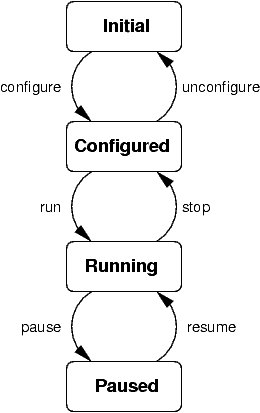
\includegraphics[scale=0.7]{online-fsm}
\end{center}
\caption{A máquina de estados finitos utilizada por todos os componentes do
TDAQ e detetores do ATLAS.}
\label{fig:online-fsm}
\end{figure}

Este pacote também provê uma interface gráfica, escrita em Java, para o
acionamento e verificação de todas as partes do sistema de filtragem e
aquisição de dados, indicando prontamente problemas ou encaminhando avisos ao
operador do \eng{run}. 

%Na Figura~\ref{fig:playdaq} é possível ver algumas
%imagens desta interface. A imagem na parte superior mostra a janela de
%controle central. Outras abas existem e podem ser utilizadas para acessar
%outras informações, como o estado do equipamento ou a taxa de operação de cada
%processador do sistema.

%\begin{figure}
%\begin{center}
%
\includegraphics[scale=1]{missing}
%\end{center}
%\caption{Algumas janelas da interface ao usuário do Sistema \eng{online}.}
%\label{fig:playdaq}
%\end{figure}

\paragraph{Bancos de dados:} contêm pacotes para a \idx{configuração} do TDAQ e
detetores. Os pacotes de configuração existem para propiciar parâmetros de
configuração do sistema, sua descrição e acesso e registro operacional de
informações durante a aquisição de dados. Há também componentes que provêm
acesso de leitura e escrita a bancos de dados que descrevem as condições do
feixe provido pelo LHC e do detetor.

Como no caso do pacote de controle, existem ferramentas para a manipulação e
verificação dos bancos de dados produzidos pelo usuário, que podem facilmente
chegar a dezenas de megabytes em sua versão final, uma vez que englobará a
configuração de milhares de componentes. Atualmente, somente uma das
interfaces de operação a banco de dados está disponível e é baseada na
utilização de arquivos locais, uma vez que o código para o acesso remoto de
bancos de dados não está implementado ainda. Os arquivos de configuração são
descritos em XML (\eng{eXtended Markup Language}) e podem ser manipulados
diretamente por usuários experientes.

\paragraph{Compartilhamento de informação:} contém pacotes para o
compartilhamento de informação no TDAQ. Os componentes destes pacotes podem
anunciar erros, publicar estados, estatística e histogramas construídos pelos
sub-sistemas do TDAQ e pelos detetores. Há um conjunto de interfaces gráficas
para a monitoração do Sistema de Filtragem do ATLAS, que podem ser acessadas
através da linha de comando em ambientes apropriadamente configurados.

%A Figura~\ref{fig:daqmonitor} exibe uma das possibilidades de
%monitoração. Nesta janela estamos observando algumas aplicações sendo
%processadas em diferentes nós de um sistema de teste.

%\begin{figure}
%\begin{center}
%
\includegraphics[scale=1]{missing}
%\end{center}
%\caption{Uma das interfaces gráficas do sistema de monitoração do DAQ exibindo
%o estado atual de alguns aplicativos.}
%\label{fig:daqmonitor}
%\end{figure}

\subsection{O Sistema de Fluxo de Dados}
\label{sec:dataflow}

O Sistema de Fluxo de Dados (do inglês \eng{Dataflow}, DF) do DAQ é
encarregado da transmissão correta e coerente dos dados do detetor, garantindo
a menor quantidade de tempo morto possível, dentro das expectativas do
experimento \cite{aa:chep-2003-2, aa:rt-2003, aa:tns-2004-3}. A
Figura~\ref{fig:dfbasic} define os componentes deste sub-sistema. Os sinais de
entrada, como podem ser observados nesta figura, são providos pelo LVL1 e
ROD's. Nesta figura, as caixas representam processadores enquanto as linhas
conectando-os representam conexões de rede (neste caso, \eng{gigabit} ou
\eng{10-gigabit} ethernet). Próximo aos nós de processamento, há uma
estimativa da quantidade destes tipos de processadores que serão necessárias
para manter a taxa de operação de 100 kHz \cite{hlt-tdr}.

\begin{figure}
\begin{center}
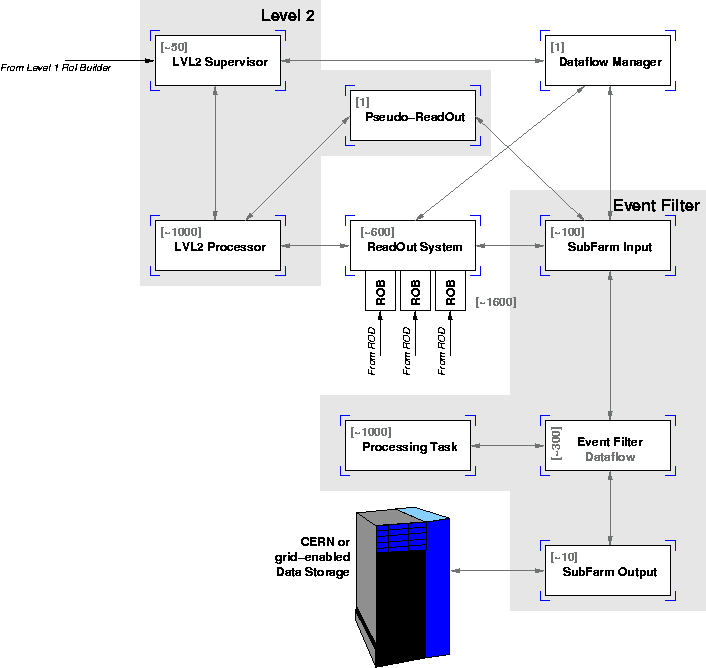
\includegraphics[scale=0.65]{dfbasic}
\end{center}
\caption{Os componentes do DF e suas interconexões.}
\label{fig:dfbasic}
\end{figure}

A seqüência de funcionamento se dá da seguinte forma: o Supervisor do LVL2
(L2SV) recebe uma mensagem do RoIB do LVL1 indicando a ocorrência de um evento
interessante e aprovado por este nível. Somente há um RoIB no sistema, que
envia para o primeiro Supervisor do LVL2 disponível a mensagem sobre o
evento. Cada Supervisor mantém um conjunto de Unidades de Processamento do
LVL2 (do inglês \eng{LVL2 Processing Unit}, L2PU) em sua lista de nós
supervisionados. Logicamente atrelado a cada L2PU há uma fila de eventos que
foram recentemente alocados para processamento. O L2SV localiza a L2PU com
menos eventos atribuídos e envia a mensagem do LVL1 para este processador.

A L2PU decodifica a mensagem enviada pelo L2SV e analisa as regiões do detetor
de que precisará para processar o evento. O tamanho e a quantidade de dados
que a L2PU necessitará para processar o evento depende dos algoritmos que são
lá executados e, portanto, este processador tem livre arbítrio na quantidade e
qualidade dos dados que irá requisitar. Para coletar os dados, a L2PU computa
o número e a localização dos ROB's que são necessários e encaminha um pedido
de dados prontamente ao Sistema de Leitura do Detetor (do inglês, \idxeng{Read
Out System}, ROS). Os ROS's afetados respondem com os dados dos ROB's
relevantes e, desta forma, a L2PU poderá classificar o evento. Após algum
intervalo de tempo necessário a análise da Física do evento, a L2PU responde
ao L2SV com um valor binário, indicando rejeição ou aceitação do evento. Se o
evento for aceito, a L2PU também envia um diagnóstico do que foi encontrado no
evento para dentro de um pseudo-ROS (pROS), que permitirá a anexação desta
informação ao evento final.

A segunda parte do processamento do evento nos altos níveis de filtragem é
iniciada por uma mensagem do L2SV ao Gerente do Fluxo de Dados (do inglês,
\eng{Dataflow Manager}, DFM), indicando o destino de todos os eventos até
então aprovados pelo LVL1. No caso de um determinado evento ser
desconsiderado, o DFM envia uma mensagem para o ROS indicando que este deverá
apagá-lo dos \eng{buffers} ou, caso contrário, enviará uma mensagem indicando
ao processador de construção de eventos (\eng{SubFarm Input}, SFI) que deverá
coletar os fragmentos do evento. O SFI então envia mensagens a cada um dos
ROS's no sistema e requer todas as informações disponíveis para o evento de
interesse. O objetivo do SFI é aglutinar todas as partes do evento em um único
espaço de memória, liberando as partes anteriores do sistema do encargo do
gerenciamento deste mesmo espaço.

Uma vez construído, o evento é guardado em uma pilha lógica dentro do SFI que
aguarda um pedido de um Gerente do Filtro de Eventos (do inglês, \eng{Event
Filter Dataflow Manager}, EFD), indicando que está disponível para processar
mais um evento. Este evento é transferido integralmente para o EFD neste
momento. O EFD, de forma análoga ao L2SV, verificará a Unidade de
Processamento (\eng{Processing Task}, PT) disponível e a alocará para tratar
as informações deste evento. Neste momento, todo o evento (com seus dados) é
disponibilizado à PT que poderá levar mais tempo processando o evento que sua
análoga no LVL2, dado a taxa reduzida de eventos remanescentes. Se aprovado, o
evento é encaminhado a um processador de saída (\eng{SubFarm Output}, SFO),
que coopera com o sistema de gravação de dados na disponibilização dos eventos
colhidos pelo DAQ.

O sistema também é equipado com dispositivos que garantem o funcionamento de
cada componente na falha de outros ou quando algum nó ou nós começam a
responder mais lentamente provocando congestionamentos. Para funcionar
plenamente, o \eng{Dataflow} está montado sobre as bases do Sistema
\eng{Online}, que provê as ferramentas de controle e configuração necessárias
para operar uma cadeia de aquisição completa.

\subsubsection{Ferramentas do \eng{Dataflow}}
\label{sec:dftools}

Para se projetar um conjunto de aplicações que funcionem coerentemente é
necessário partir de uma base funcional comum. Desta forma, optou-se pelo
projeto e construção de um conjunto de ferramentas que fornecem uma base para
o desenvolvimento das aplicações do DF. Estas ferramentas incluem:

\begin{itemize}
\item Ferramentas para isolamento do Sistema Operacional: reúnem um
conjunto de bibliotecas que executam funções primárias como a criação de
tarefas (para ambientes multi-tarefa), relógios e primitivas como filas
protegidas. Esta camada de funções também isola, dentro do possível, variações
no sistema operacional de alterações no código das aplicações do DF;

\item Ferramentas para troca de mensagem: provêm uma interface simples para a
troca de mensagens entre aplicações. Os canais de comunicação são
configuráveis permitindo o tráfego (transparente) de dados diretamente sobre
pacotes \eng{ethernet}, UDP ou TCP. Este pacote também engloba ferramentas
para a codificação e decodificação dos dados provenientes dos detetores.

\item Ferramentas para configuração: provêm interfaces para a configuração dos
aplicativos utilizando o Sistema \eng{Online};

\item Ferramentas para controle e relatório de erros: permitem o envio de
mensagens de erro e depuração para os nós de controle da cadeia de
aquisição. Este conjunto de ferramentas também imbute os aplicativos, nos
moldes da máquina de estados apresentada na Figura~\ref{fig:online-fsm}.
\end{itemize}

Para aumentar a qualidade dos programas desenvolvidos e a manutenção a
longo prazo (o experimento deve operar por 10 anos), optou-se por utilizar
técnicas de orientação à objetos (OO) aplicadas sobre C++. Alguns problemas,
e.g. ineficiência da utilização dos \eng{containers}-padrão da biblioteca
padrão (\eng{Standard Template Libraries}, STL) C++ em ambientes multi-tarefa,
advieram desta decisão \cite{aa:chep-2003}. De fato, a alocação de memória
implementada pelos compiladores da linha GCC \cite{web:gcc, web:gcc-stl} visa
a otimização da alocação de memória por processo enquanto em ambientes
multi-tarefas (do inglês \eng{multi-threading}) é necessário a utilização de
pilhas separadas para cada tarefa. A solução neste caso foi a adoção de
alocadores mais eficientes para este propósito, que não fazem parte do padrão
C++.

\subsection{Fluxo de dados e a arquitetura no LVL2}
\label{sec:lvl2arch}

Em específico para este trabalho, a arquitetura e \eng{modus operandi} do
segundo nível de filtragem do experimento são de especial atenção. É possível
observar na Figura~\ref{fig:lvl2arch} um esquema da troca de mensagens das
aplicações no LVL2, como anteriormente indicado na área acinzentada da
Figura~\ref{fig:dfbasic}. Nesta figura, as linhas tracejadas indicam mensagens
de controle do sistema e as linhas cheias, as mensagens que carregam dados do
detetor ou resultados da operação de filtragem. Inicialmente, o Supervisor do
LVL2 recebe uma mensagem contendo as informações das RoI encontradas pelo
LVL1. As RoI's equivalem a objetos encontrados, seja nos detetores de múons ou
nos calorímetros, com energia mínima para a ativação dos subseqüentes níveis
de filtragem. Esta mensagem é chamada de Resultado do LVL1, e abreviadamente
de ``L1R''. A mensagem que chega ao L2SV representa, portanto, uma avaliação
do evento com uma qualidade equivalente à visibilidade que o LVL1 tem do
detetor. Para continuar com a avaliação do evento, o L2SV alocará uma L2PU que
esteja sob sua guarda para processá-lo.

\begin{figure}
\begin{center}
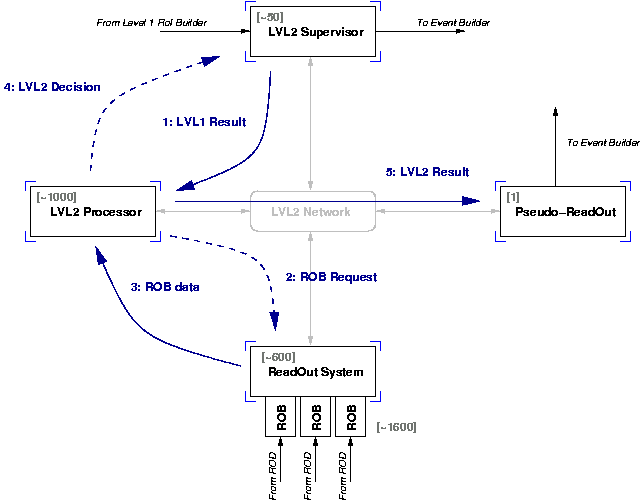
\includegraphics[scale=0.7]{lvl2arch}
\end{center}
\caption{A ordem das mensagens trocadas pelas aplicações do LVL2.}
\label{fig:lvl2arch}
\end{figure}

A L2PU processa eventos por RoI. Para cada RoI encontrada em um resultado do
LVL1, a L2PU requisitará os dados ao redor do objeto e avaliará novamente o
objeto, levando em conta a máxima granularidade do detetor ao redor daquele
ponto. Se o objeto encontrado pelo LVL1 tiver sido achado através de sua
interação com o calorímetro, o LVL2 requisitará inicialmente os dados deste
sub-detetor. Caso o objeto tenha sido encontrado nos detetores de múons, o
processamento começará a partir deste sub-sistema. O processamento de cada
evento na L2PU se dá de forma seqüencial. Para cada RoI destacada pelo LVL1 é
feita uma confirmação da análise do LVL1 contando com a melhor precisão
disponível para os dados avaliados e possíveis validações cruzadas, levando-se
em conta dados dos detetores internos. Se a RoI for rejeitada, o processamento
é abortado e imediatamente uma mensagem de controle é enviada ao L2SV
indicando um evento inválido. Caso as diversas etapas de processamento se
confirmem ao longo da análise do evento, a resposta ao L2SV é atrasada até que
o evento seja confirmado em última instância ou rejeitado no meio do
processamento. Nota-se aqui que eventos interessantes terão maior tempo de
processamento que eventos ordinários, já que os últimos serão rejeitados assim
que possível, enquanto que os primeiros terão que ser aprovados por todos os
critérios de processamento no LVL2. O processamento como um todo continua
requisitando dados à medida do necessário, aos diversos ROS's, até que a L2PU
possa concluir, com baixíssima probabilidade de erro, se o evento deve ser
aprovado ou rejeitado.

O L2SV opera de forma indiferente à rejeição ou aceitação do evento por um
Processador do LVL2, já que repassará todas as mensagens, possivelmente
agrupadas para melhorar o desempenho da comunicação de pacotes, ao DFM. Por
outro lado, a cadeia de processamento para a L2PU se dá de forma ligeiramente
diferente se tiver um evento confirmado. Caso o evento seja rejeitado, somente
uma mensagem de controle é enviada ao L2SV. De outra forma a L2PU deverá,
antes da mensagem de controle, enviar um extrato completo das operações
executadas a um \eng{buffer} indicado na Figura~\ref{fig:lvl2arch} por
\eng{Pseudo ReadOut}, PROS. Este único processador do sistema opera como um ROS,
porém, ao invés de coletar dados de ROB's, armazena os resultados
(diagnósticos) de eventos bem-sucedidos do LVL2, servindo estes resultados a
um SFI quando o evento é construído. É desta forma que o resultado das
operações do LVL2 poderá chegar ao Filtro de Eventos. O PROS é uma aplicação
bastante simples que fornece 2 interfaces (lógicas) de rede. A primeira coleta
os dados de todas as L2PU's do sistema e a segunda responde a requisições dos
SFI's que desejam construir os eventos aprovados.

Após enviar o resultado das operações do LVL2 (L2R) ao PROS, a L2PU poderá
enviar a mensagem de aceitação ao L2SV. Desta forma garante-se que a
construção do evento operará corretamente, uma vez que o PROS não receberá um
pedido para enviar o L2R antes de o ter recebido. O processamento prosseguirá
desta forma por períodos que durarão até 10 horas e, portanto, erros de
programação e, principalmente, vazamentos de memória são proibitivos neste
árduo ambiente.

O orçamento do sistema é otimizado para canalizar a maior quantidade de
recursos possível em poder de classificação de eventos. Portanto, a relação
entre o número de L2PU's e os demais nós de processamento deve ser tão grande
quanto possível. Atualmente estima-se que serão necessários cerca de 1.000
processadores (operando como L2PU's) para suportar a taxa de entrada de
eventos de 100 kHz. Dado o paralelismo inerente ao processo, cada L2PU deverá
processar um evento em não mais do que 10 milissegundos, i.e., cada um poderá
suportar uma taxa de 100 Hz.

\subsubsection{Arquitetura da L2PU}
\label{sec:l2puarch}

A arquitetura da L2PU pode ser melhor descrita através da
Figura~\ref{fig:l2puarch}, onde é possível observar três componentes primários:

\begin{itemize}
\item Tarefa de Entrada (\eng{input thread}): Canaliza o recebimento de dados
dentro da L2PU. Cada tipo de mensagem recebida está associada a um manuseador
(\eng{handler}) distinto que especifica o destino a ser dado à mensagem
recebida. Por exemplo, mensagens do L2SV indicando resultados do LVL1 são
encaminhadas para uma pilha protegida;

\item Pilha Protegida: Controla o acesso concorrente das tarefas processadoras
(\eng{worker threads}) aos resultados do LVL1 depositados na L2PU;

\item Tarefas Processadoras: É onde o processamento (seqüencial) de cada
evento é feito. Cada tarefa possui um Coletor de Dados que é responsável pela
comunicação com os ROS's disponíveis para reunir os dados necessários a cada
passo do processamento de um evento.
\end{itemize}

\begin{figure}
\begin{center}
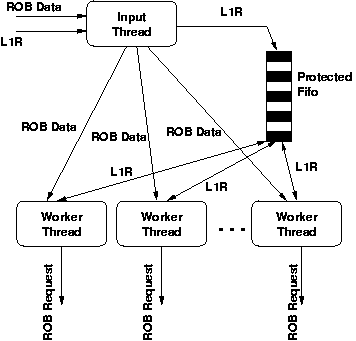
\includegraphics[scale=0.8]{l2puarch}
\end{center}
\caption{A arquitetura da L2PU.}
\label{fig:l2puarch}
\end{figure}

Ao receber um L1R do Supervisor, a tarefa de entrada irá colocá-lo numa pilha
tipo FIFO (\eng{First In First Out}) protegida ao acesso concorrente da cada
uma das tarefas processadoras. As tarefas concorrem na aquisição de um L1R
para iniciar o processamento e, caso sucedam, saem do modo de espera, onde
praticamente não consomem a CPU do sistema hospedeiro, e iniciam a
discriminação do evento. Para isso, requisitam dados aos ROS's disponíveis que
enviarão, dentro de suas possibilidades, os fragmentos da RoI equivalentes ao
subdetetor de interesse. É possível que determinados ROS's não consigam
responder ao tempo máximo de espera da L2PU e, neste caso, o evento deve ser
processado com dados faltantes. Há outras possibilidades que podem comprometer
a integridade dos dados que serão finalmente manipulados na L2PU, já que a
cadeia de aquisição, passando pela eletrônica de aquisição acoplada ao
detetor, os ROB's e finalmente os ROS's, podem apresentar inúmeros tipos de
falhas que resultarão na perda dos dados analisados pela L2PU, total ou
parcialmente. Os algoritmos de discriminação devem estar preparados para estas
anomalias de funcionamento e devem ser construídos para consumir o mínimo
possível de dados, já que além da maior probabilidade de falhas, mais dados
também significam maior banda passante necessária à rede que interliga estes
dois nós de processamento.

Os fragmentos de RoI (e também do detetor) que são carregados pela L2PU são
armazenados e transmitidos em um formato particular e uma biblioteca de
codificação e decodificação \cite{aa:ef-urd, aa:ef-ooad} está disponível para
este propósito. Os dados não são somente decodificados, mas também
rearranjados e calibrados antes do uso, o que pode consumir grande parte do
tempo de processamento (10 ms) no LVL2.

O L2R juntamente com a decisão do LVL2 são enviados diretamente das tarefas
processadoras ao L2SV e ao PROS sem a intervenção de outros componentes dentro
da L2PU.

\subsubsection{Parâmetros de \eng{Hardware} do DAQ}

A escolha da tecnologia de processamento, tal qual aquela empregada para a
rede de interconexão destes nós, é um parâmetro vital para viabilização do
Sistema de Aquisição de Dados do ATLAS. Diversos aspectos devem ser
considerados:

\begin{itemize}
\item Econômico: Deve-se maximizar os recursos disponíveis. Desta forma,
deseja-se despender o mínimo necessário em recursos para a compra de
equipamento. Por ``mínimo necessário'' entende-se o mínimo necessário para
operar, de forma cômoda, o experimento por 10 anos;

\item Operacionais: O equipamento deve ter sua operabilidade maximizada. Deve
ser relativamente fácil repor componentes ou realizar atualizações que não
impliquem na reposição de toda a cadeia de aquisição. A manutenção e operação
dos programas deve ser acessível a novos usuários.
\end{itemize}

Por estas razões decidiu-se pela utilização de equipamentos disponíveis no
mercado de comodidades atual: PC's operando sobre redes padrão (\eng{gigabit}
ou 10-\eng{gigabit}) ethernet. O sistema operacional escolhido foi Linux. A
razão desta escolha se deve a estabilidade do sistema em operação contínua e a
confiabilidade dos módulos para conexão em rede. A utilização de um sistema
operacional aberto, gratuitamente distribuído, também facilita o
desenvolvimento de \eng{drivers} especializados para atividades específicas.

Para maximizar a operabilidade e diminuir o custo, pretende-se adquirir
máquinas duplamente ou quadruplamente processadas com memória compartilhada
(arquitetura SMP, do inglês \eng{Symmetric Multi-Processor}). Esta arquitetura
apresenta várias vantegens:

\begin{itemize}
\item Para cada 2 ou 4 processadores, somente 1 disco e 2 interfaces de rede
serão necessárias\footnote{Uma das interfaces de rede é alocada para sinais e
dados de controle enquanto a outra funciona exclusivamente para o tráfego de
dados do detetor. Nesta configuração, somente uma das duas interfaces de rede
necessita de uma banda passante maior, a interface por onde trafegarão os
dados obtidos no detetor.}. Desta forma, não há somente economia de espaço e
dinheiro, mas também no tamanho da rede final que será projetada;

\item Há também economia de energia durante a operação e, principalmente,
durante o momento de ligação das máquinas. A conexão concomitante de 2.500
discos rígidos pode acarretar problemas de super-aquecimento do \eng{cluster}
e quedas de tensão em outros pontos do sistema.
\end{itemize}

A arquitetura da L2PU, apresentada na Seção~\ref{sec:l2puarch}, deriva desta
escolha do equipamento. Uma vez que somente uma das interfaces estará
disponível para o tráfego de dados, a utilização de mais tarefas para esta
atividade torna-se desnecessária. O número de tarefas processadoras, no
entanto, deve ser otimizado para que o sistema atinja o seu desempenho máximo.

\subsection{Análise Funcional do Fluxo de Dados no LVL2}
\label{sec:lvl2work}

Para avaliar a correta operação dos diversos processos que compõem o LVL2, é
necessário operar os diversos componentes em uma bancada de teste (do inglês
\eng{testbed}). Por razões econômicas, o sistema em sua escala de produção
(cerca de 2.500 nós de processamentos) somente estará disponível em uma data
próxima ao início de operação do detetor. Por outro lado, a transferência na
data de compra também possibilita a aquisição de processadores mais potentes
pelo mesmo custo. Desta forma, as \eng{testbeds} disponíveis para teste, ainda
que representando o estado da arte dos equipamentos escolhidos, são de tamanho
reduzido se comparadas ao sistema final.

De forma a qualificar a avaliação de cada componente, faz-se necessário criar
condições de operação que satisfaçam o modelo de operação final. Com relação
ao LVL2, muitos modelos foram explorados \cite{aa:tns-2004} ao longo de 2 anos
de testes. Estes modelos e a verificação do funcionamento coerente desta parte
do sistema de aquisição encontram-se sintetizados nesta seção \cite{hlt-tdr}.

Como será detalhado mais adiante, na Seção~\ref{sec:hlt}, os módulos que
executam a análise da Física de interesse são carregados dinamicamente na
L2PU, através de parâmetros de configuração disponíveis ao operador do
experimento. Esta estratégia permite que o sistema de fluxo de dados seja
testado independentemente dos algoritmos de filtragem, paralelizando o
desenvolvimento \cite{aa:tns-2004-2} e reduzindo significativamente as
possibilidades de falha devido a componentes que não relevem a natureza dos
testes. Para os processos descritos nesta seção, foram utilizados emuladores
dos componentes de discriminação, que podem simular a aquisição de dados de
RoI's e até o tempo de processamento entre cada tomada de dados, possivelmente
em múltiplos passos. Este bloco emulador é sintonizado para caracterizar os
parâmetros normais de operação do LVL2.

\subsubsection{Parâmetros Críticos do Sistema de Leitura}

Um dos parâmetros que se deseja investigar é a capacidade da L2PU de coletar
dados do sistema de leitura, neste caso representado pelos diversos
ROS's. Como colocado anteriormente, ao processar um resultado do L1R, a L2PU
começa por confirmar o resultado encontrado no nível precedente, utilizando,
para isso, a granularidade máxima do detetor ao redor da RoI. O tamanho da RoI
dependerá diretamente dos valores discriminantes que devem ser
encontrados. Algumas modalidades de algoritmos podem requerer mais dados e,
portanto, aumentar significativamente o tráfego de dados na rede. Algoritmos
mais eficientes tenderão a consumir dados em pequenas parcelas, minimizando o
tempo de rejeição necessária para cada evento do ruído de fundo. É possível,
em todos os casos, adquirir pequenas parcelas de dados inicialmente e aumentar
o campo de atuação do algoritmo à medida que o evento não é rejeitado. Por
outro lado, também é possível compartimentalizar a aquisição de dados por
sub-detetores. Cada estágio do processamento seqüencial do evento adquirirá,
neste modelo, dados de diferentes camadas do ATLAS. A solução ótima está
provavelmente na utilização das duas técnicas, ou seja, o consumo parcelado de
dados para cada sub-detetor com rejeição assim que possível. Uma rejeição
rápida garante mais tempo para o processamento de eventos realmente
interessantes e minimiza o tráfego de rede.

Cada L2PU, como visto anteriormente, mantém uma fila tipo FIFO com eventos
alocados pelo Supervisor do LVL2. A maximização do tempo de processamento
disponível depende, portanto, da não-escassez de eventos nesta fila, uma vez
que com a fila vazia, uma ou mais das tarefas processadoras serão
bloqueadas. Desta forma, o L2SV é sintonizado cuidadosamente para que esta
situação nunca ocorra.

Ainda que o número e o tamanho médio das RoI's dependam da Física a ser
avaliada, o fator de concentração de ROB's (o número de ROB's que deve ser
lido de cada ROS) é um parâmetro que deve ser otimizado. Variações de
desempenho nesta área indicam melhores geometrias para a interconexão do
sistema de leitura do detetor e a rede que liga o LVL2. Por outro lado, o
número ótimo de tarefas processadoras operando dentro de cada L2PU dependerá
do tempo-morto despendido durante a aquisição de dados e do número de
processadores disponível em cada máquina. Em máquinas duplamente processadas,
por exemplo, o número ótimo de tarefas processadoras deve estar entre 3 e 4,
já que o uso de um número menor deste tipo de tarefas implicará na
subutilização do poder de processamento de cada nó.

Medidas foram realizadas variando-se parâmetros críticos para o desempenho da
coleção de dados para RoI's. A contribuição gerada pela coleção de dados para
uma RoI, ao tempo de processamento de uma L2PU em função do tamanho da RoI e o
número de ROS's na qual a RoI está distribuída, é mostrada na
Figura~\ref{fig:tns-4fig}. Estes testes foram executados em uma bancada com
apenas um L2SV, doze ROS's e uma L2PU. Todos os nós nesta bancada de teste são
PC's duplamente processados com Intel/Xeon's de 2,2 GHz e 1 \eng{gigabyte} de
memória RAM, interconectados por uma chave padrão \eng{gigabit} ethernet. Na
figura, o eixo vertical é possível observar a taxa de processamento inversa de
um L2SV com uma única L2PU sob seu controle. Este parâmetro representa o tempo
médio que cada evento levou para ser inteiramente processado pelo LVL2, ou
seja:

\begin{figure}
\begin{center}
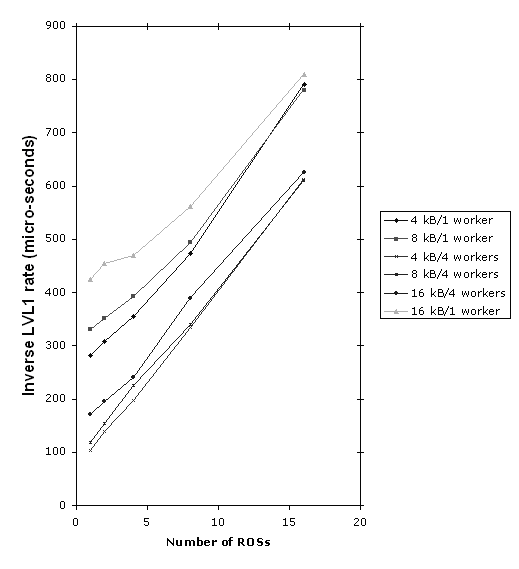
\includegraphics{tns/4fig}
\end{center}
\caption{Desempenho da coleção de dados de RoI para várias combinações de
tamanhos de RoI (em bytes) e tarefas processadoras.}
\label{fig:tns-4fig}
\end{figure}

\begin{enumerate}
\item O tempo de envio do resultado do LVL1 para o L2PU;
\item A aquisição do resultado pela tarefa processadora;
\item O mapeamento da RoI nos ROB's de interesse;
\item A aquisição dos dados dos ROS's;
\item A resposta para o L2SV indicando aceitação ou rejeição.
\end{enumerate}

Neste caso, o tempo de processamento para os dados foi ajustado para zero. A
resposta da L2PU ao L2SV é sempre negativa (para evitar o envio do L2R ao
PROS). 

No eixo horizontal da Figura~\ref{fig:tns-4fig}, é possível observar o número
de ROS's que contribuíram para os dados na RoI. O conjunto de medidas
apresentado nesta figura corresponde a valores de tamanhos de RoI realísticos
para dados partindo da seção e.m. do calorímetro, representando este o pior
dos casos. Para este sub-detetor, estima-se que a RoI para os dados de todas
as três camadas do detetor encontre-se espalhada por 13 a 16 ROB's e tenha um
tamanho total, em média, de 16 \eng{kilobytes}. É possível notar, através
deste gráfico, que o tempo de coleção de dados contribui, no pior dos casos,
em apenas 10\% do tempo de processamento médio estimado para cada evento no
LVL2 (10 milissegundos).

Podemos também notar que o aumento no número de tarefas processadoras de 1
para 4 modifica significativamente o perfil do tempo-morto gasto na aquisição
de dados, já que não haverá esperas espontâneas no sistema como colocado
anteriormente neste texto. No caso de 4 tarefas processadoras, o tempo de
coleção de dados está na ordem de 600 microssegundos. Podemos também observar
que com maior distribuição de dados no sistema (mais ROS's), o tempo de
coleção de dados de uma RoI aumentará numa relação aproximadamente linear, o
que casa bastante bem com o modelo OO apresentado. A minimização do número de
ROS's é portanto desejável para um tempo-morto menor.

Na Figura~\ref{fig:tns-5fig} observa-se o desempenho de uma única L2PU contra
a taxa de operação de um L2SV invertida para um número variável de tarefas
processadoras. Neste teste o tamanho da RoI está fixo em 16
\eng{kilobytes}. As diferentes curvas representam a mesma RoI sendo coletada
de 2, 4, 8 ou 16 ROS's. Por exemplo, a curva superior representa os resultados
para coletar uma RoI de 16 \eng{kilobytes} de 16 ROS's (1 \eng{kilobyte} por
ROS). O resultado indica que o número ótimo de tarefas processadoras para esta
bancada de testes (sistemas duplamente processados) é de, aproximadamente,
três e é independente do número de ROS's dos quais os dados da RoI estão sendo
coletados. Ademais, os resultados mostram que, para as condições deste teste,
e para 3 tarefas processadoras, a coleção de dados contribui com menos de 10
\% do tempo de processamento médio esperado no LVL2 de 10 ms. Isto concorda
com o estudo anterior.

\begin{figure}
\begin{center}
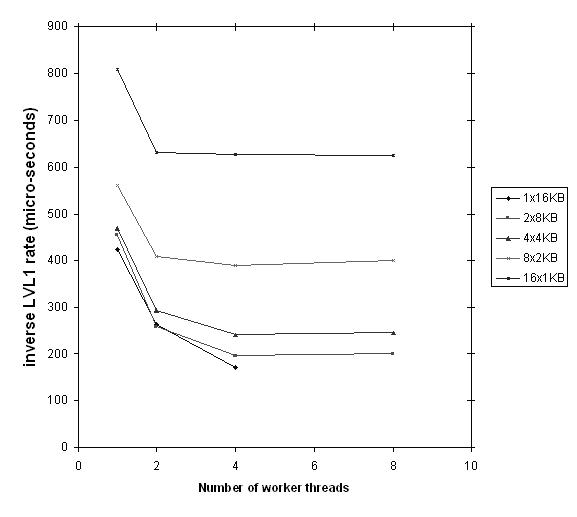
\includegraphics[scale=0.9]{tns/5fig}
\end{center}
\caption{A taxa inversa em um L2SV para uma única L2PU funcionando com
diferentes números de tarefas processadoras.}
\label{fig:tns-5fig}
\end{figure}

\subsubsection{Escalabilidade do LVL2}

Os testes apresentados até agora mostraram a taxa com a qual uma L2PU pode
coletar dados, se não estiver equipada com algoritmos de discriminação de
eventos. O desempenho atingido depende do tamanho da RoI, o fator de
concentração de ROB's por ROS's e do número de tarefas processadoras
disponível neste processador. Para o sistema de aquisição como um todo, no
entanto, é também necessário demonstrar que, quando muitas L2PU's estão
coletando dados ao mesmo tempo do mesmo conjunto de ROS's, o desempenho da
coleção de RoI's não degrada de forma inaceitável.

Para este teste, L2PU's não equipadas de algoritmos de filtragem reais foram
usadas novamente e, por esta razão, deve ser notado que a taxa de envio de
mensagens de cada um destes nós estará operando num patamar bastante acima do
que o sistema real necessitará. Para estes testes, cada L2PU estará gerando
\textbf{10 vezes} mais tráfego que o esperado no sistema final. De forma
análoga e aditiva, o número de ROS's do sistema também não é ideal, devido a
baixa disponibilidade de equipamento para testes. É, portanto, necessário
garantir que a taxa de requisições de dados para cada ROS não exceda um valor
limite que mascararia quaisquer resultados obtidos.

Estes testes foram executados em uma bancada com três L2SV's, quatro ROS's e
até onze L2PU's. Todos os nós nesta bancada de teste são PC's, na mesma
configuração de antes, interconectados por uma chave padrão \eng{gigabit}
ethernet. Para este teste, cada ROS foi configurado para emular 12 conexões
com ROB's, gerando um total de 48 ROB's para este teste. Para cada requisição,
a L2PU escolhe um dos 48 ROB's aleatoriamente e um número de ROB's com
numeração consecutiva. Por exemplo, no caso em que cada RoI consista de 6
ROB's, a L2PU seleciona o primeiro aleatoriamente e completa o pedido com
outros 5 ROB's, cuja a numeração sucede o primero ROB. Se o último ROB fosse
selecionado, o algoritmo voltaria ao primeiro ROB disponível
(\eng{wrap-around}).

A Figura~\ref{fig:tns-6fig} traz os resultados sintetizados desta
bancada. Nesta figura é possível observar a taxa de eventos média tratados em
cada L2PU em função do número de L2PU's usadas no teste para uma RoI
distribuída por 1, 6 ou 24 ROB's (com cerca de 1,5 \eng{kilobytes} por
ROB). Observa-se na figura que a taxa por L2PU diminui quando o número de
L2PU's aumenta, por aproximadamente 20\% para 1 ROB por RoI e aproximadamente
40\% para 24 ROB's por RoI. Entretanto, com 11 L2PU's configurados na bancada,
a taxa de requisições por ROS é de 17 kHz para 1 ROB por RoI e de 8 kHz para
24 ROB's por RoI. Estas duas situações representam uma sobrecarga jamais
atingível no sistema final. A taxa total de requisições de dados de RoI nesta
pequena bancada de testes é de 70 kHz e 11 kHz para os dois números de ROB's
por RoI indicados.

\begin{figure}
\begin{center}
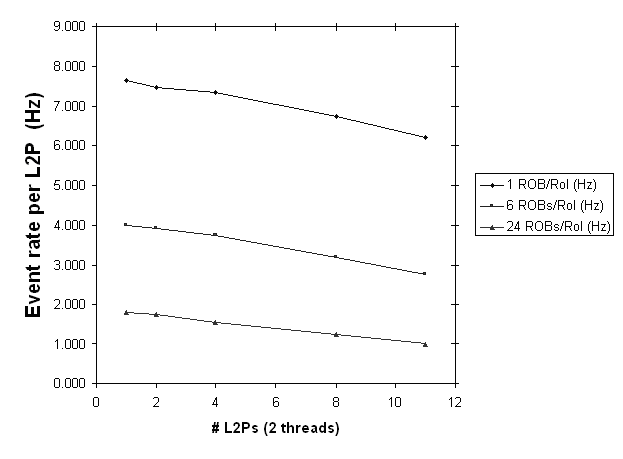
\includegraphics[scale=0.9]{tns/6fig}
\end{center}
\caption{A taxa de eventos média para cada L2PU em função do número de
L2PU's no sistema para diferentes números de ROB's por RoI. Cada ROB contribui
com um montante igual dos dados da RoI.}
\label{fig:tns-6fig}
\end{figure}

Na Figura~\ref{fig:tns-scale-burn} é possível observar os resultados de uma
bancada de testes equivalente contendo 1, 2, 4 e 8 L2PU's. Porém, desta vez,
ajustou-se o tempo de processamento emulado para cada evento em 1
milissegundo. Isto representa apenas a décima parte do esperado no sistema
final. Nesta figura, é possível observar um bom escalonamento do
sistema. Dadas as extremas condições recriadas nestas bancadas, é razoável
assumir que a escalabilidade do sistema final se mostrará aceitável às
condições do DAQ.

\begin{figure}
\begin{center}
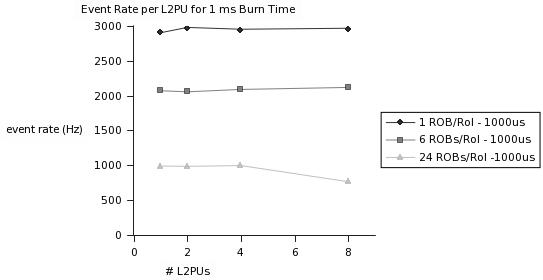
\includegraphics[scale=0.7]{tns/scale-1msburn}
\end{center}
\caption{A taxa de eventos média para cada L2PU em função do número de L2PU's
no sistema. O tempo de processamento emulado para cada evento é de 1 ms.}
\label{fig:tns-scale-burn} 
\end{figure}

Observa-se na Figura~\ref{fig:tns-7fig} a taxa sustentada por um L2SV em
função do número de L2PU's sob seu controle. Nesta bancada, o nó de
processamento rodando o L2SV está conectado através de uma chave \eng{gigabit}
ethernet, com um número de outras máquinas rodando o código da L2PU sem
algorítmos de discriminação carregados e sem coletar dados dos ROS's. Este é
portanto um teste extremo, visto que as L2PU's vão responder o mais rápido
possível a cada requisição de processamento de eventos feita pelo L2SV. Como
pode ser visto pela figura, um único L2SV pode sustentar a taxa de 32 kHz
enquanto distribuindo L1R's para apenas uma das L2PU's sob seu controle e a
dependência no número de L2PU's está na ordem de 1\%. Desta forma, tomando-se
como ponto de partida a implementação do sistema de fluxo de dados e as
máquinas, cerca de 10 L2SV's seriam capazes de suprir a taxa de entrada do
LVL2. Há, todavia, outros fatores não considerados nesta suposição, tais como
robustez e a conexão com o DFM, que certamente penaliza a taxa de
processamento. Levando-se todos os pontos em questão, parece ser razoável
contar com a presença de 30 a 50 L2SV's no sistema final.

\begin{figure}
\begin{center}
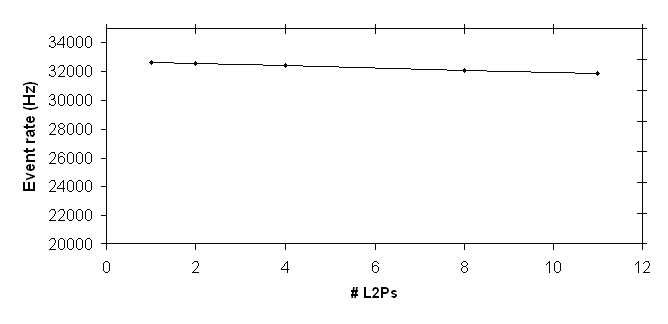
\includegraphics[scale=0.8]{tns/7fig}
\end{center}
\caption{A taxa sustentada por L2SV com o aumento de L2PU's no sistema.}
\label{fig:tns-7fig}
\end{figure}

Os testes aqui descritos descrevem e comprovam o funcionamento da
infraestrutura que permite o acoplamento dos algoritmos que executam a
discriminação dos eventos lidos pelo detetor ATLAS. A eficiência destes mesmos
algoritmos é de extrema importância para o desempenho final do sistema de
filtragem. Um conjunto de procedimentos ineficaz e lento será mais oneroso
economicamente e também tecnicamente, já que a qualidade dos eventos
finalmente aprovados se torna duvidosa.

\subsection{Altos Níveis de Filtragem e seus algoritmos}
\label{sec:hlt}

A infraestrutura de seleção de eventos dos Altos Níveis de Filtragem constitui
o ambiente de processamento para os algoritmos de discriminação do DAQ. Esta
infraestrutura é comum ao LVL2 e ao EF e é composta de 4 partes distintas. O
Gerente do HLT (ou, do inglês, \eng{Steering}) agenda os algoritmos do HLT
correspondentes ao tipo de evento que está sendo analisado. Informações sobre
quantidades físicas específicas a um evento são trocadas através de
componentes do Modelo de Dados do Evento (do inglês \eng{Event Data Model},
EDM). Durante o processamento, os dados gerados são guardados e acessados
através de um Gerente de Dados (do inglês, \eng{Data Manager}, DM). Isto
permite transparência às escolhas de plataforma de armazenamento e tecnologia
utilizadas para executar as operações de filtragem. Os algoritmos do HLT
propriamente ditos reconstróem quantidades relativas aos eventos ou confirmam
hipóteses através de quantidades previamente calculadas. A
Figura~\ref{fig:hlt-arch} ilustra o relacionamento entre estes macrossistemas
do HLT com alguns exemplos de classes representativas.

\begin{figure}
\begin{center}
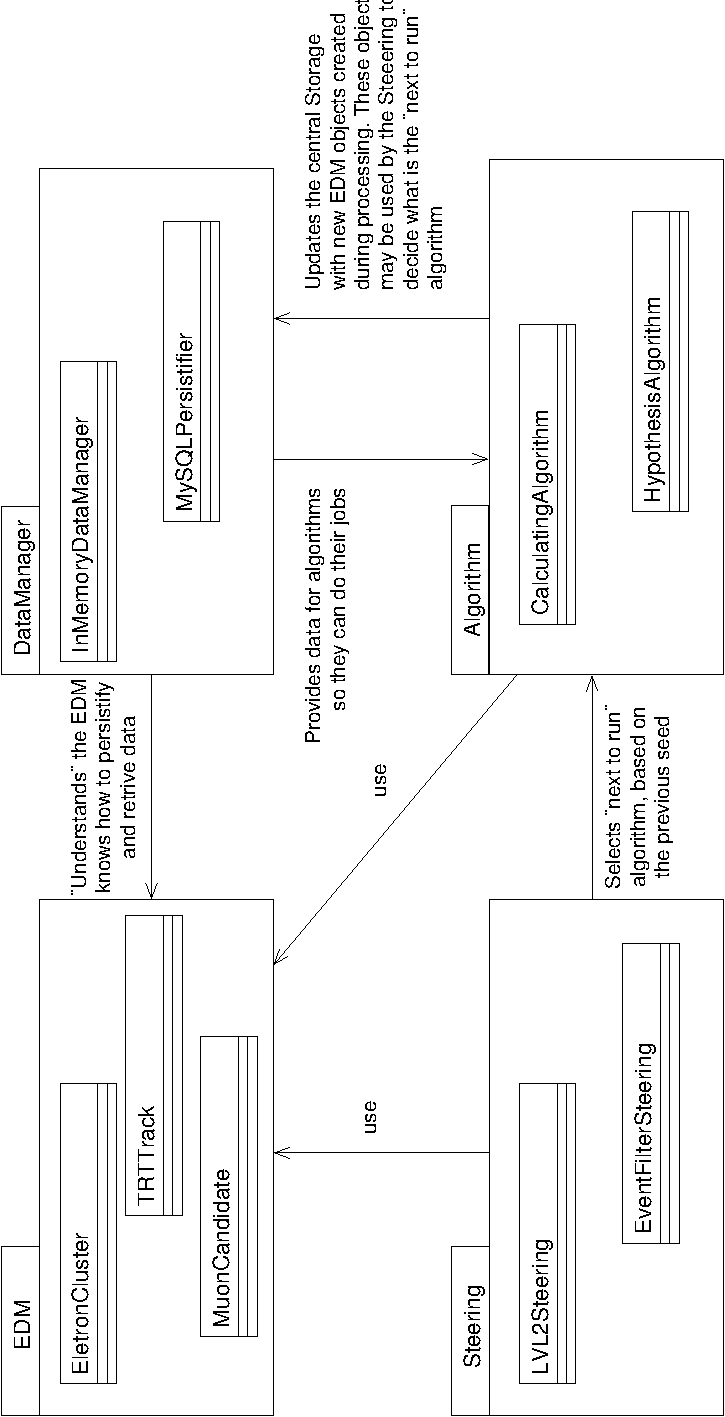
\includegraphics[scale=0.8,angle=90]{hlt-arch}
\end{center}
\caption[Relação entre os macrossistemas do HLT.]{Relação entre os
macrossistemas do HLT. Extraído de \cite{hlt-tdr}.}
\label{fig:hlt-arch}
\end{figure}

Uma vez que o propósito do \eng{software} de discriminação de eventos do HLT é
a seleção de eventos, ele deve executar de maneira eficiente e confiável no
ambiente do DAQ/Fluxo de Dados. Os componentes críticos para a seleção devem
ser portados ao ambiente \eng{offline} para seu desenvolvimento e
teste. Provendo um conjunto básico de interfaces para ambos os cenários, o HLT
garante a consistência para o desenvolvimento do sistema de
filtragem. Ademais, alguns estudos \cite{jb:e-gamma} mostram que um grande
custo computacional pode ser economizado com a otimização global do sistema de
filtragem quanto à ordem e a qualidade dos algoritmos executados. A existência
de uma infraestrutura comum também facilita este tipo de estudo.

Uma vez que o Filtro de Eventos provê um ambiente de computação praticamente
igual ao ambiente \eng{offline}, o conjunto de rotinas do HLT é naturalmente
baseado no ambiente de análise \eng{offline}, Athena, que por sua vez é
baseado na infraestrutura de análise física Gaudi \cite{athena:home-page,
athena:devel-guide}. Esta estratégia permite a reutilização do Gerente de
Dados, do EDM, da descrição dos detetores e de muitos algoritmos que já se
encontram desenvolvidos por esta comunidade. Apenas o Gerente do HLT
(\eng{Steering}) e determinados algoritmos restam como desenvolvimentos
específicos a este sub-sistema. No caso específico do LVL2, um enfoque similar
torna-se mais complexo, já que o processo de seleção ocorre em múltiplas
tarefas concorrentes às unidades de processamento disponíveis e restrições
mais severas tornam-se necessárias. Ainda que os algoritmos destinados ao LVL2
sejam especialmente desenvolvidos para esta plataforma (devido às restrições
no desempenho), eles utilizam o mesmo EDM e descrição do detetor presentes no
EF e \eng{offline}. A utilização transparente de tais componentes é possível e
uma implementação comum da infraestrutura do HLT para ambos o LVL2 e o EF pode
ser realizada se a mesma interface estiver disponível para o LVL2. Esta
comunalidade é provida pelo Gerente do HLT no LVL2 (\eng{LVL2 Steering
Controller}, L2SC).

\subsubsection{O L2SC}

O L2SC é componente de \eng{software} que faz a interface entre a L2PU, que
provê acesso aos dados do detetor através dos ROS's e dos ROB's, e os
componentes do HLT. O propósito do L2SC está em 3 aspectos: permitir que a
L2PU seja hospedeira do \eng{software} do HLT e sua controladora primária;
permitir a reutilização do mesmo conjunto de componentes (algoritmos, EDM,
etc) entre o LVL2, o EF e \eng{offline}; prover um mecanismo de transmissão
dos resultados do LVL1 e do LVL2 entre o DAQ e \eng{software} de seleção de
eventos. Por esta razão, da mesma forma que a L2PU, o L2SC deve seguir a
máquina de estados descrita na Figura~\ref{fig:online-fsm}, ativando seus
múltiplos estágios de configuração e processamento conforme requerido pelo
operador do DAQ. Um aspecto importante deste enfoque é que o acesso aos dados
providos pelo LVL2 é totalmente gerenciado pela base funcional do Sistema de
Fluxo de Dados. O L2SC não precisa interagir diretamente com a tarefa de
entrada ou quaisquer outros componentes da aplicação hospedeira.

A Figura~\ref{fig:l2sc-interaction} ilustra a seqüência de interações do L2SC
com a L2PU e com alguns dos componentes pertinentes do HLT. Durante a fase de
configuração, parâmetros de execução e dados atrelados às condições de deteção
são obtidos de bancos de dados externos através desta interface. Estes dados
são posteriormente utilizados para configurar o sistema de seleção de eventos
e componentes associados. Três estados são mostrados: \textit{Configuração},
\textit{Inicialização} e \textit{Término}. A área em cinza mostra interações
que ocorrem em tarefas processadoras (concorrentes).

\begin{figure}
\begin{center}
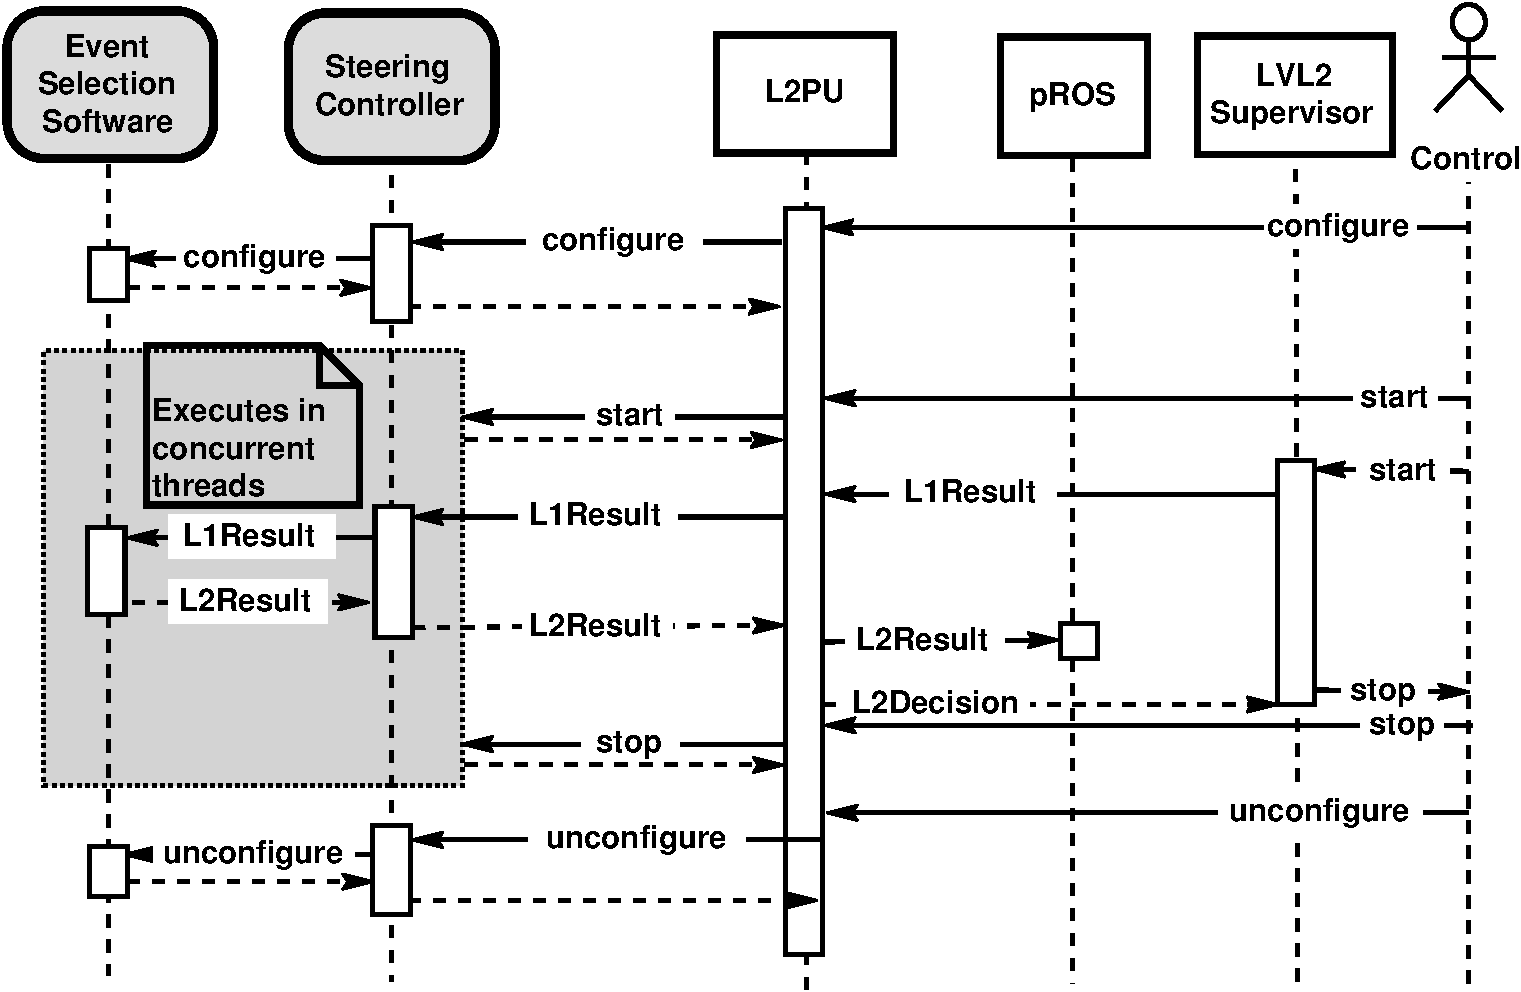
\includegraphics[scale=0.55]{tns2/2fig}
\end{center}
\caption{A seqüência de interações do L2SC com o L2PU e o \eng{software} de
seleção de eventos.}
\label{fig:l2sc-interaction}
\end{figure}

Após a \textit{Inicialização} o L2SC recebe uma chamada \texttt{Execute Event}
com um resultado do LVL1 como argumento. O resultado do processamento do
evento é automaticamente retornado como resultado do LVL2 para a L2PU. O
comando \textit{Término} termina a execução dos algoritmos e produz um sumário
do período de execução.

\subsubsection{Modelo de Desenvolvimento do L2SC}

Uma vez que as mesmas interfaces estão disponíveis no LVL2 e no EF, o código
desenvolvido no ambiente \eng{offline} pode ser diretamente carregado em seu
formato binário nestes processadores. Para o LVL2, no entanto, o desenvolvedor
deve seguir um conjunto de regras simples \cite{aa:lvl2-coding} durante o
ciclo de desenvolvimento para produzir código seguro ao acesso concorrente (do
inglês \eng{thread-safe}) ou serviços compatíveis com a criação automática de
múltiplas cópias na L2PU. Não deve ser necessário utilizar trancas
(\eng{locks}) ou \eng{mutexes} para adaptar o código a este ambiente
multi-tarefas. Para respeitar as retrições no tempo de execução para o LVL2, o
número e o tipo de serviços disponíveis estão restritos ao mínimo necessário,
sendo este um subconjunto do serviços disponíveis no EF e \eng{offline}. Desta
forma é sempre possível mover um componente do LVL2 para executar no EF ou até
\eng{offline}. A movimentação de componentes no sentido oposto, no entanto,
deve observar as restrições de operação no LVL2. 

\subsubsection{Desempenho do HLT}

Após integrar o L2SC com o Sistema de Fluxo de Dados, testes de desempenho e
robustez form conduzidos em uma máquina duplamente processada com AMD/Athon's
de 1,533 GHz. O L2SC rodou por mais de 50 horas com três tarefas
processadoras. O protótipo executou sem problemas aparentes (\eng{dead-locks},
vazamentos de memória, etc.) em nós simples ou duplamente processados,
mostrando a segurança ao acesso concorrente. Medidas do desempenho desta
infraestrutura exibiram um \eng{overhead} de 13 $\mu$s por evento. Este valor
foi estimado comparando-se o número de eventos por segundo uma L2PU pode
manusear quando operando com e sem o L2SC e executando um algoritmo simples
(primeira e segunda linhas da Tabela~\ref{tab:l2sc}). Esta tabela também
mostra a taxa de processamento obtida quando, adicionalmente, o resultado do
LVL1 é transferido para o Gerente de Dados. O valor de \eng{overhead}
mencionado inclui toda a infraestrutura Athena para agendar e executar os
algoritmos e os serviços básicos. Estes valores são basedos em execuções de,
no mínimo, 100.000 eventos. Escalonamento quase perfeito da latência medida
foi observado quando o tempo de execução dos algoritmos era variada com um
ciclo de processamento fictício de 0 a 8 milissegundos em configurações
distintas, indicando que o \eng{overhead} por evento introduzido pelo L2SC
seja independente do tempo de execução observado.

\begin{table}
\begin{center}
\begin{tabular}{|l|c|c|}
\hline
Configuração do Protótipo & Taxa Medida & \eng{Overhead} por Evento \\
\hline
\hline
L2PU & 21,7 kHz & 46 $\mu$s \\
\hline
L2PU + L2SC & 17,0 kHz & 59 $\mu$s \\
\hline
L2PU + L2SC + Gerente de Dados & 15,3 kHz & 65 $\mu$s \\
\hline
\end{tabular}
\end{center}
\caption{Taxas de processamento em um sistema duplamente processado AMD-Athlon 1,533 GHz.}
\label{tab:l2sc}
\end{table}

Na seqüência, testes mais complexos foram feitos com uma fatia completa do
sistema de seleção para elétrons e fótons ($e^-/\gamma$). Estes testes
continham o Gerente do HLT, um algoritmo decodificador do resultado do LVL1,
agendamento de algoritmos para o LVL2 e o envio dos resultados do
processamento do LVL2 para o EF. O Gerente de Dados, o EDM e a descrição dos
detetores para os calorímetros do ATLAS foram também carregados no conjunto de
teste, que estava funcionando sobre uma bancada que consistia de três nós de
processamento: dois duplamente processados (o AMD/Athlon anteriormente
mencionado e um Intel/Xeon de 2,2 GHz) hospedando o ROS e a L2PU
respectivamente, interconectados por
\eng{Gigabit} ethernet e um nó com apenas um processador (Intel/Pentium 4 de
2,2 GHz) para hospedar o L2SV. O algoritmo de extração de características para
dados do calorímetro foi especialmente desenvolvido para o LVL2, utilizando
toda a infraestrutura disponível mencionada anteriormente. Para este teste, 95
\% dos eventos foram processados em menos de 5 milissegundos para uma amostra
simulada de jatos duplos (\eng{di-jets}) em baixa luminosidade, para um
tamanho de RoI de $\Delta\eta \times \Delta\phi = 0,3 \times 0,3$. A
Figura~\ref{fig:l2sc-mu} exibe resultados similares para uma fatia completa de
seleção para múons. Nesta figura é possível ver que as contribuições, em ordem
decrescente, para o tempo de processamento total de cada evento são
pré-processamento dos dados e sua conversão para o EDM, os \eng{overheads} da
infraestrutura provida pelo HLT (\eng{Steering}), processamento do algoritmo
de extração de características (denotado por \texttt{muFast} na figura) e o
tempo de acesso dos dados pela rede. As curvas mostram que, neste exemplo, o
processamento termina, para 95 \% dos eventos, em menos de 2 milissegundos. A
amostra de dados analisada consiste de múons com massa de 200 GeV em um
ambiente de alta luminosidade do feixe. Esta amostra, que é simulada através
de processos de Monte Carlo, inclui um ruído de fundo equivalente ao que será
observado na caverna do ATLAS em sua disposição final.

\begin{figure}
\begin{center}
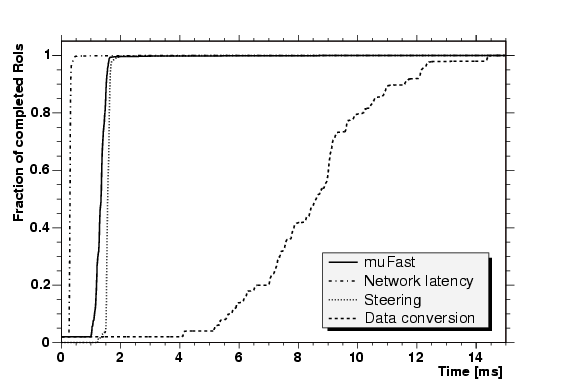
\includegraphics[scale=0.65]{tns2/4fig}
\end{center}
\caption{As principais contribuições para o tempo de processamento mostradas
como integrais para a fatia completa do sistema de seleção para RoI's de
múons.}
\label{fig:l2sc-mu}
\end{figure}

\typeout{ *************** End of file trigger.tex *************** }

%% Hello emacs, this is -*- latex -*-
\typeout{ ====================================================================}
\typeout{ This is file baseline.tex, created at 18-Aug-2006 }
\typeout{ Maintained by Andre Anjos <Andre.dos.Anjos@cern.ch> }
\typeout{ ====================================================================}

\chapter{Filtragem baseada em calorimetria no experimento ATLAS}
\label{chap:baseline}

Sistemas de calorimetria são habitualmente construídos com forma e leitura
segmentada de maneira que possam ser usados diretamente na dete\-ção de
par\-tí\-culas. Isto é possível uma vez que muitos processos interessantes são
distinguíveis pela forma com que depositam energia à medida que interagem com
estes detetores, tanto de forma radial quanto longitudinal
\cite{wigmans-book}. Cada segmento ou célula de um calorímetro contém a
informação de energia depositada por uma par\-tí\-cula ou conjunto de
par\-tí\-culas que interagiu com o detetor naquela área espe\-cí\-fica. A
seg\-men\-ta\-ção destes instrumentos dependerá da Física do experimento e
também, normalmente, do eixo de dispersão das partículas de interesse.

Algoritmos de dete\-ção são normalmente concebidos por especialistas em
Calorimetria que compreendam os diferentes perfis de intera\-ção para a
Fí\-sica de interesse. O primeiro passo é definir um processo de redu\-ção de
dimensionalidade, de acordo com os processos que se deseja detetar, ainda que
levando-se em consideração à velocidade requerida na deteção. Quanto menor o
tempo disponível à deteção, maior a compressão a ser realizada de forma a
simplificar este processo. Este pré-processamento para a compressão dos dados
ou Extração de Características (do inglês, \eng{Feature Extraction} ou FEx) é,
em geral, feito com perda de informação do perfil de deposição, mas de forma a
manter as principais características do objeto que se deseja detetar. Em
seguida, tendo por base simulações ou dados reais da Física de interesse,
define-se um conjunto de cortes por métodos com conhecimento da informação
\eng{a priori} que maximizem a probabilidade de deteção das partículas
interessantes.

O Sistema de Filtragem \eng{online} do experimento ATLAS deverá prover uma
seleção de eventos muito eficiente e desprovida de tendências, mantendo o
potencial de descoberta do detetor. Deve ser extremamente flexível, de forma a
operar no ambiente desafiador do LHC, com até 23 colisões inelásticas por
interação, 14~TeV de energia no centro de massa e apenas 25~ns (40~MHz) entre
colisões sucessivas. Além disso, deve prover critérios de seleção robustos e,
onde possível, redundantes. É altamente desejável a rejeição de canais
ruidosos, não interessantes ou falsos o mais rápido possível, de forma a
otimizar o uso dos recursos computacionais disponíveis.

Para trazer uma eficiência compatível com este árduo ambiente, o Sistema de
Filtragem fará uso de um enfoque baseado na \textbf{inclusão} para a seleção
\eng{online}, garantindo assim um conjunto de \eng{triggers} ótimo para a nova
Física. O critério da inclusão tem por objetivo selecionar um conjunto de
fenômenos físicos baseados em características comuns entre eles, que ainda
sejam claramente distinguíveis dentro do ruidoso ambiente produzido pelo
acelerador. Com este objetivo, o Sistema de Filtragem estará sendo disparado
para eventos que contenham assinaturas baseadas em objetos simples ou duplos
com alto valor de momento transverso. Neste contexto, objetos com alto valor
de momento transverso são, entre outros, \eng{léptons} com carga e com momento
transverso acima de $\sim$10 GeV \cite{hlt-tdr}.

Neste capítulo, fazemos uma análise do processo de filtragem de elétrons a ser
conduzido no Sistema de Filtragem do experimento ATLAS. Como em muitos outros
experimentos em Física de Altas Energias \cite{abolins-calor-2000,
monteiro-calor-1999}, este sistema é seccionado em níveis que realizam o
processo de filtragem em passos com complexidade e tempo de execução
crescentes. O primeiro dos níveis é normalmente implementado em
\eng{hardware}, para atender as demandas de tempo do feixe, enquanto que os
demais em \eng{software}, maximizando a flexibilidade. Em particular, atenção
será dada à definição do funcionamento do Primeiro e Nível de Filtragem (LVL1)
com relação a deteção de elétrons e, em seguida, o sistema desenvolvido
atualmente para o LVL2. Finalmente, uma caracterização dos dados disponíveis
segundo as premissas desenvolvidas neste capítulo é estabelecida como base de
comparação ao restando do trabalho.

\section{Objetos de interesse e RoI's}

Foi visto no Capítulo~\ref{chap:trigger} que o Primeiro Nível de Filtragem do
ATLAS define, para objetos encontrados seja nos Calorímetros ou nos Detetores
de Múons, regiões de interesse onde objetos relevantes tenham sido
observados. Para cada objeto interessante, a região aproximada de interação do
objeto com o detetor é anotada e repassada aos demais níveis de filtragem, no
caso da aprovação do evento pelo LVL1. Este processo define as Regiões de
Interesse ou RoI's, que guiarão o processo de seleção nos Altos Níveis de
Filtragem (do inglês, \eng{High-Level Triggers} ou HLT).

De fato, dadas as condições do feixe provido pelo LHC, múltiplos objetos
poderão ser detetados a cada evento. Porém, quando um ou mais objetos
detetados ativam a aceitação do evento, o LVL1 marca o dado de forma especial,
distinguindo este objeto como primário, em contraste com aqueles que também
foram detetados, mas não fizeram objeto da aceitação deste nível de
filtragem. O processo de deteção no LVL2 começa por uma confirmação dos
objetos primários detetados pelo LVL1, utilizando-se da granularidade
completada do detetor ao redor da RoI. Em seguida, o processo de filtragem
poderá, eventualmente, ser refinado ainda neste nível de filtragem ou mais a
frente, no EF, complementando-se a análise com base em RoIs secundárias. Este
sistema de filtragem \eng{online} baseado em RoIs é um elemento de
diferenciação do experimento ATLAS \cite{atlas-tp}, sendo esta a primeira vez
que é implementado em um ambiente em Física de Altas Energias.

A Tabela~\ref{tab:l1-rates} apresenta as taxas (simuladas) para as diferentes
assinaturas de interesse, ou conjuntos de objetos primários, que serão
entregues pelo LVL1~\cite{hlt-tdr} ao HLT, encabeçados pelo LVL2, para a
luminosidade inicial de $2\times10^{33}cm^{-2}s^{-1}$. Este valor de
luminosidade está cerca de uma ordem de magnitude abaixo do valor final de
operação do LHC, de $\approx 10^{34}cm^{-2}s^{-1}$. Com o aumento da
luminosidade do feixe, a relação entre as taxas ou até o tipo das assinaturas
nesta tabela sofrerá alterações tendo em vista a mudança na probabilidade de
ocorrência de fenômenos mais raros.

\begin{table}
\caption{Taxas de saídas para as assinaturas reconhecidas pelo LVL1,
para a luminosidade de pico inicial de $2\times10^{33}cm^{-2}s^{-1}$. Dados
baseados em uma simulação do LVL1.}
\label{tab:l1-rates}
\begin{center}
\begin{sideways}
\begin{tabular}{|l|l|r|}
\hline
\textbf{Assinatura do LVL1} & \textbf{Codinome} & \textbf{Taxa (kHz)} \\ \hline
e.m., 25 GeV, com isolamento & \texttt{EM25i} & 12 \\ \hline
2 $\times$ e.m., 15 GeV, com isolamento & \texttt{2EM15i} & 4 \\ \hline
Múon, 20 GeV & \texttt{MU20} & 0.8 \\ \hline
2 $\times$ múon, 6 GeV & \texttt{2MU6} & 0.2 \\ \hline
Jato, 200 GeV & \texttt{J200} & 0.2 \\ \hline
3 $\times$ jato, 90 GeV & \texttt{3J90} & 0.2 \\ \hline
4 $\times$ jato, 65 GeV & \texttt{4J65} & 0.2 \\ \hline
Jato, 60 GeV $+$ \textit{Missing Energy}, 60 GeV & \texttt{J60} $+$
\texttt{XE60} & 0.4 \\ \hline
$\tau$, 25 GeV, com isolamento $+$ \textit{Missing Energy}, 30 GeV &
\texttt{TAU25i} $+$ \texttt{XE30} & 2 \\
\hline
Múon, 10 GeV $+$ e.m., 15 GeV, com isolamento & \texttt{MU10} $+$ \texttt{EM15i} & 0.1 \\ \hline
Outros disparos (pré-escalonados, aleatórios, calibração, monitoração) & -- & 5 \\
\hline
Total & -- & $\sim$25 \\ \hline
\end{tabular}
\end{sideways}
\end{center}
\end{table}

Nota-se que, aproximadamente, 16 dos 25 kHz (i.e. $\sim$65\% das assinaturas)
entregues pelo LVL1 conterão objetos tipo e.m.. Estes objetos são assim
classificados por representarem elétrons \textbf{ou} fótons, que interagem com
os detetores a partir de interações eletromagnéticas em vez das componentes
hadrônicas presentes em outros casos. Em algumas das assinaturas, exige-se que
o objeto seja \emph{isolado}. Isto quer dizer que a quantidade de energia no
centro do objeto deverá manter uma razão mínima com relação a energia
depositada em sua periferia, como ficará claro mais a frente.

\section{Análise do sistema de filtragem com relação à Física}

A Figura~\ref{fig:trigger-physics} apresenta um diagrama esquemático que
despreza as interfaces em \eng{hardware} propostas pela construção do Sistema
de Filtragem e tenta enfocar melhor o problema do ponto de vista da análise
dos canais físicos. De cima para baixo, indica-se o tráfego de mensagens até a
completa aceitação de um evento por parte do Sistema de Filtragem.

\begin{figure}
\begin{center}
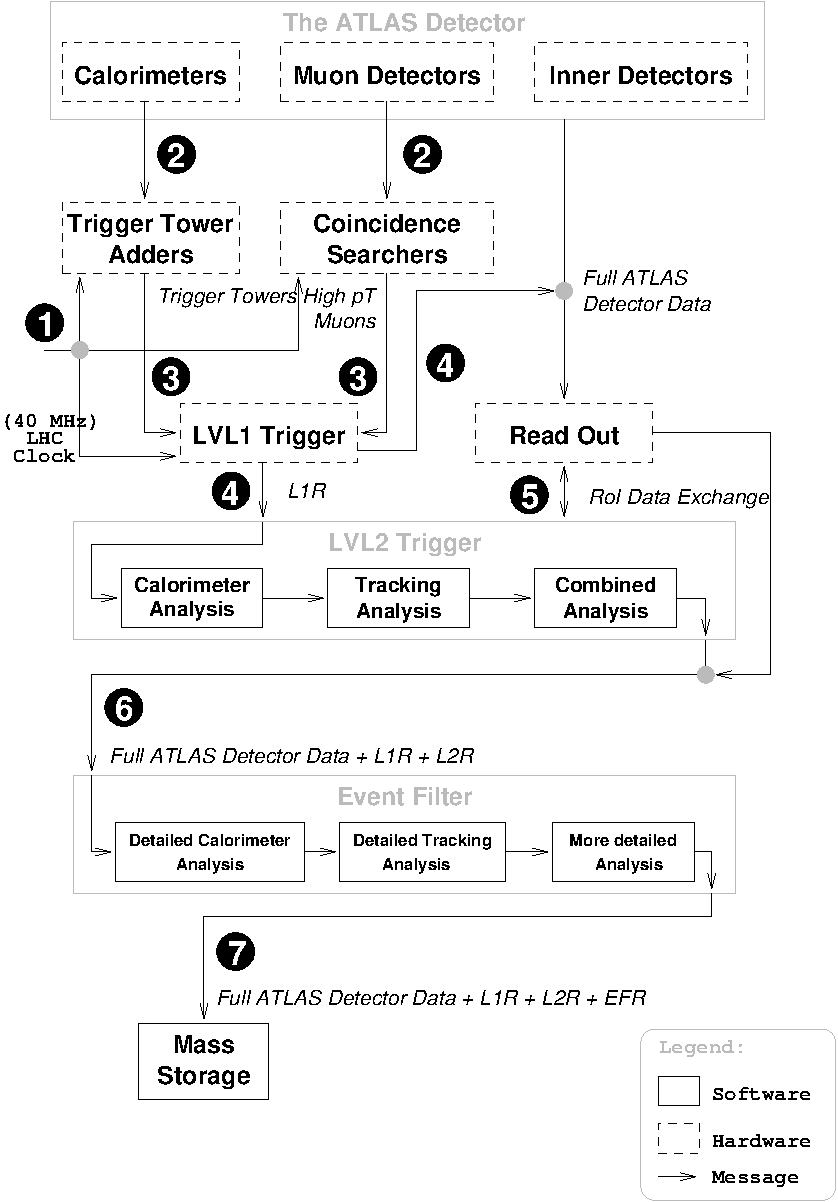
\includegraphics[scale=0.9]{trigger-physics}
\end{center}
\caption{Diagrama esquemático do Sistema de Filtragem do Experimento ATLAS
segundo suas funções de filtragem.}
\label{fig:trigger-physics}
\end{figure}

O processamento começa à medida que o LVL1 recebe o sinal do LHC acusando o
iminente cruzamento de pacotes (do inglês \eng{Bunch Crossing}) no ponto de
impacto (mensagem \ding{182}). Uma janela de aquisição de alguns nanossegundos
fará com que o Sistema de Leitura do LVL1 registre o evento (mensagem
\ding{183}). Os sistemas de pré-processamento são ativados em seguida.

No caso dos Calorímetros, somadores rápidos \cite{seixas:adder} agrupam as
informações das células dos calorímetros e.m. e hadrônicos, formando, para
cada seção, uma matriz de dados com granularidade reduzida
\cite{l1-tdr}. Estas macro-células ou ``torres'' de filtragem (do inglês,
\eng{Trigger Towers}, ou TT) agrupam os dados formando elementos com tamanho
igual a $0,1\times0,1$ no plano $\eta\times\phi$. Estes dois planos com
granularidade minimizada são varridos pelos diversos processadores do LVL1 e
os objetos de interesse, ou seja RoI's, localizados no detetor. Um processo
análogo é conduzido tendo por base os detetores de múons, com o objetivo de
encontrar objetos deste tipo (mensagem \ding{184}).

No final do processamento pelo LVL1, rapidamente depois da colisão, e no caso
de tratar de um evento interessante, uma mensagem contendo a localização dos
objetos encontrados por este nível de filtragem e variáveis indicando as
assinaturas pelo qual o evento foi aprovado, é repassada ao LVL2
(mensagem \ding{185}). Esta mensagem é chamada de Resultado do LVL1 (do inglês
\eng{LVL1 Result}) ou L1R, como visto na Seção~\ref{sec:lvl2arch}. Nota-se que
o L1R pode conter múltiplas assinaturas em um único evento, no caso deste
conter elementos que confirmem mais de uma das linhas da
Tabela~\ref{tab:l1-rates}. Ademais, múltiplas RoI's secundárias podem estar
presentes na lista de objetos na mensagem. Em paralelo ao envio da mensagem em
direção ao LVL2, o LVL1 indica ao sistema de aquisição de dados (marcado na
figura como \eng{Read Out}) que carregue todos os dados do detetor em seus
\eng{buffers}.

O processamento no LVL2 é seqüencial. Ao receber um L1R, o Coordenador de
Execução do LVL2 (do inglês, \eng{Steering}) chamará um algoritmo de filtragem
para a confirmação do disparo do LVL1. O algoritmo em questão poderá
transferir, do sistema de leitura do detetor, a quantidade de dados que achar
necessária, ao redor da RoI, de forma a processá-la (mensagem \ding{186}). Se
não for possível rejeitar a assinatura do LVL1, o \eng{Steering} poderá chamar
mais e mais algoritmos até que o evento seja rejeitado ou definitivamente
aprovado ao Terceiro Nível de Filtragem ou Filtro de Eventos (do inglês
\eng{Event Filter} ou EF). Neste último caso, de forma equivalente à relação
entre o LVL1 e o LVL2, o LVL2 enviará um sumário indicando a razão da
aceitação do evento ao EF (mensagem \ding{187}). Este sumário contém valores
refinados de energia, momento e localização dos objetos explorados no contexto
LVL2. Analogamente ao resultado do LVL1, o resultado do LVL2 é chamado L2R (do
inglês {LVL2 Result}). Espera-se que o LVL2 atinja uma redução da taxa de
eventos de aproximadamente 25 vezes, de forma que o EF possa operar a uma taxa
de apenas alguns (1 ou 2)~kHz. O tempo médio de processamento para o LVL2 deve
estar na ordem dos 10~ms e para o EF, na ordem de alguns segundos, levando-se
em consideração o número de processadores disponíveis nestes níveis de
filtragem. No caso do evento ser aprovado pelo EF, é armazenado em mídia
permanente (mensagem
\ding{188}).

Os tempos de processamento-alvos representam a média de processamento por
evento. De fato, espera-se que eventos de interesse utilizem mais tempo de
processamento, enquanto que eventos pouco ou nada interessantes sejam
rapidamente descartados. Neste contexto, entende-se que, quanto menor o tempo
necessário e maior a qualidade da deteção dos diversos componentes do sistema
de filtragem, mais tempo computacional será despendido com a Física de
interesse e menos recursos com eventos que representem Física ordinária.

Diferentemente do LVL2, a análise no EF começa com 100\% dos dados do evento e
os resultados dos nível precedentes (L1R e L2R) já disponíveis na
memória. Neste nível de filtragem, correlações mais complexas podem ser feitas
entre as diferentes RoI's, e uma análise mais depurada do evento poderá ser
conduzida. Por exemplo, é possível fazer uso das RoI's secundárias para
atingir maior redução da taxa de eventos a serem registrados em mídia
permanente. Se aprovado, o evento é guardado, devidamente ``etiquetado'' e
repassado às fazendas (\eng{farms}) de processamento \eng{offline} para
posterior reconstrução.

\section{Deteção de elétrons baseada em calorimetria}
\label{sec:e-detection}

O \eng{trigger} de elétrons ou fótons para o ATLAS conterá forte contaminação
de jatos com componentes hadrônicas, que formam o ruído de fundo na deteção de
elétrons \cite{nevski-calor-1992}. Estima-se que o ruído de contaminação
original esteja na ordem de $10^6$. O LVL1 do ATLAS poderá excluir grande
parte dos jatos QCD, se as conversões hadrônicas forem importantes neste
objeto, e apenas observando a quantidade de energia hadrônica depositada na
seção de mesmo nome dos calorímetros, mas terá pouca eficiência em conversões
com menos componentes hadrônicas. Estima-se em
\cite{daqnote00-02}, que a cada 25.000 objetos do tipo e.m., aprovados pelo
LVL1, apenas 1 será um elétron ou fóton verdadeiro. Somente no LVL2, o Sistema
de Filtragem, disporá do tempo e da completa granularidade do detetor para
executar uma seleção mais criteriosa, refinando a decisão obtida no LVL1
\cite{hlt-tdr} (mas originalmente discutida em \cite{ellis-calor-1992}). O
algoritmo de calorimetria também refina a posição do objeto originalmente
determinada pelo LVL1, de forma que algoritmos de deteção de traços,
reconhecidamente menos eficientes, possam reduzir sua área de procura. Por
estas razões, a correta identificação de elétrons é de suma importância para o
experimento.

A Figura~\ref{fig:e-shower} mostra a interação de um elétron com um detetor de
traços (\eng{Cloud Chambers}) e absorvedores de chumbo. Nesta figura, é
possível observar a formação de um chuveiro de partículas que diverge,
aproximadamente de forma isotrópica, do eixo de penetração do elétron. No caso
de elétrons \cite{wigmans-book}, a dispersão é menor que no caso de jatos de
partículas, já que há uma grande probabilidade de espalhamento múltiplo (do
inglês \eng{Multiple Scattering}) causado pelas componentes hadrônicas do
conjunto de partículas. A distância de penetração é diretamente proporcional à
energia do objeto em análise \cite{leo, knoll}, ainda que, para os mesmos
valores energéticos, jatos tendam a penetrar mais profundamente nos
dispositivos.

\begin{figure}
\begin{center}
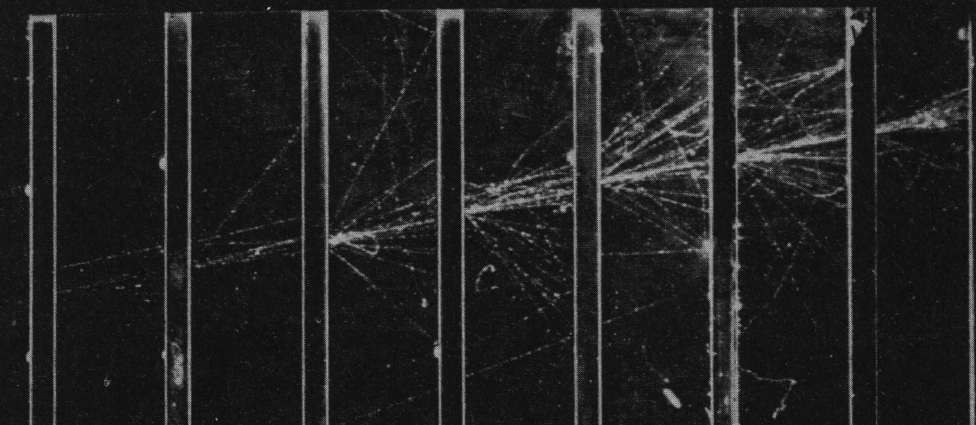
\includegraphics[scale=0.4]{e-cloud-chamber}
\end{center}
\caption{Interação de um elétron com um detetor de traços com absorvedores em
chumbo.} 
\label{fig:e-shower}
\end{figure}

%%CONSEGUIR FOTO DE UMA ROI COM O DÊNIS: ELECTRON, JET?

A deteção de elétrons beneficia-se deste conhecimento básico para
distingui-los de sua contaminação natural de jatos (e píons). Numa primeira
fase, chamada de Extração de Características, avalia-se, para uma região do
detetor, normalmente centralizada em um ponto pré-determinado, um conjunto de
valores que representem, o melhor possível, os perfis de deposição lateral (ou
radial) do objeto sendo estudado e sua penetração no aparato. Este processo
comprime\footnote{Para os fins deste trabalho define-se ``compressão'' ou
compactação a técnica pelo qual reduz-se a dimensionalidade de um sinal em um
espaço bem definido, preservando ou tentando preservar a informação relevante
que caracteriza este sinal de interesse. A transformação do espaço original
para o espaço ``comprimido'' é irreversível, salvo onde especificado.} a
informação de entrada, que normalmente possui dimensionalidade bastante
elevada (O(100)-O(1000)), para um conjunto pequeno (O(10)) de variáveis que
possam ser analisadas mais facilmente.

A questão da dimensionalidade da entrada está intimamente correlacionada com a
capacidade discriminatória do calorímetro. Quanto mais granular, maior
precisão pode ser obtida na definição de pontos de impacto e deteção de
partículas. O revés é o custo - detetores multi-segmentados são mais difíceis
e custosos de serem construídos.

No caso do experimento ATLAS (veja a Seção~\ref{sec:atlas-calo} para mais
detalhes), os calorímetros são segmentados em diversas camadas, e, camada a
camada, granularizados em células de deposição energética. A granularidade
varia camada a camada, pois cada uma delas possui um objetivo distinto de
emprego: as camadas iniciais têm por objetivo a discriminação de elétrons e
fótons e estimativa de posicionamento, as mais traseiras a deteção de
hádrons. As camadas da seção e.m. têm profundidade variante, sendo que a
segunda (EM2, a contar do zero, ou seja o pré-irradiador), tem a maior
profundidade de todas, ocupando mais de 80\% do volume total desta seção.

Para elétrons com valores energéticos até algumas dezenas de
gigaelétron-volts, espera-se que a maior parte da energia do objeto esteja
depositada nesta camada. A granularidade é bastante regular, tanto ao longo do
eixo $\eta$ quanto ao longo de $\phi$, como é possível observar na
Tabela~\ref{tab:lar}. Esta tabela também mostra o fator de compressão (ou
tamanho da torre de filtragem) $N_{\eta} \times N_{\phi}$ aplicado ao processo
de agrupamento necessário ao pré-processamento antes da análise feita pelo
LVL1.

A seção hadrônica do calorímetro é bastante menos granular. O tamanho padrão
da célula ($0,1\times0,1$ no espaço $\eta\times\phi$) foi otimizado para
detetar hádrons. Esta classe de partículas penetra mais profundamente na
matéria e desenvolve complexas cascatas ao longo da penetração, normalmente
pouco interessantes. Entretanto, devem estar contidas no espaço do detetor. O
agrupamento padrão (torre de filtragem) para o LVL1 é de $2\times2$ células.

A Figura~\ref{fig:e-jet-deposit} mostra histogramas da relação da deposição
energética na seção hadrônica e a energia total do objeto considerando-se uma
área $0,4\times0,4$ no plano $\eta\times\phi$. Os eventos considerados são
simulações de elétrons e jatos cobrindo um campo energético de algumas dezenas
de GeV até 90 GeV interagindo com os calorímetros do ATLAS. Os eventos
selecionados passaram uma simulação realística do LVL1 e portanto representam,
todos, eventos que seriam classificados como elétrons por este nível de
filtragem. Observa-se que para jatos há uma probabilidade maior de depósito na
seção hadrônica que na seção e.m..

\begin{figure}
\begin{center}
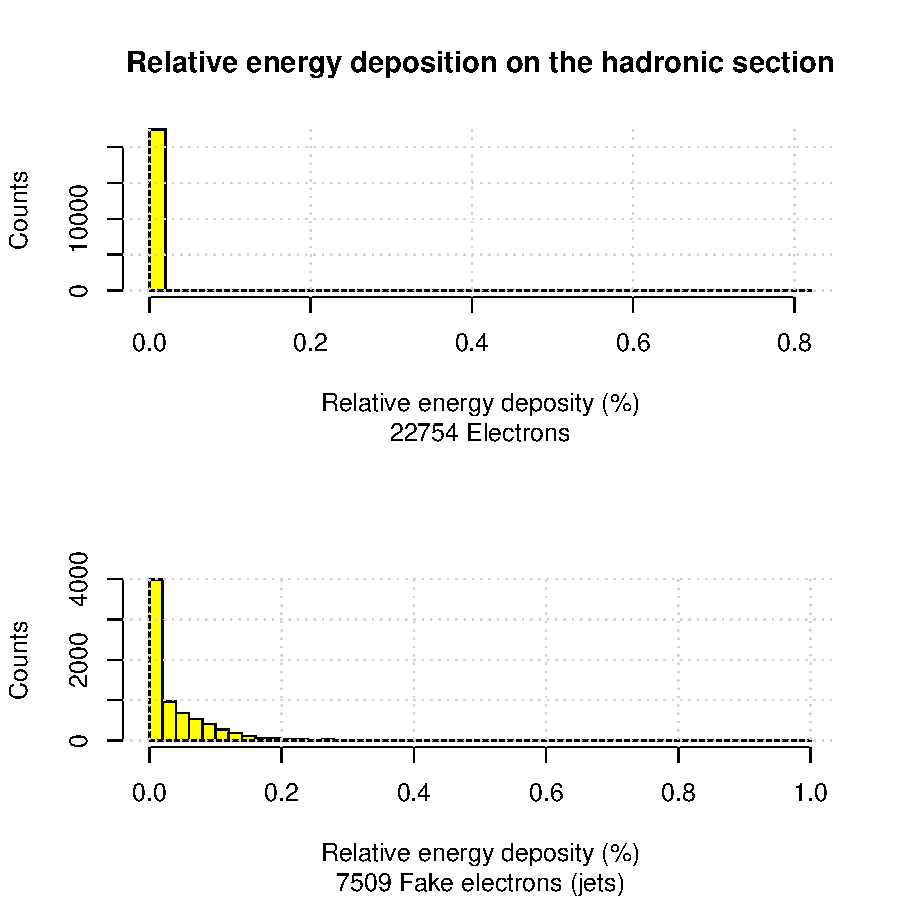
\includegraphics[scale=0.95]{em-had-percent}
\end{center}
\caption{Exemplo da relação de deposição energética na seção hadrônica e
energia total para elétrons (topo) e jatos (baixo).}
\label{fig:e-jet-deposit}
\end{figure}

Em seguida, aplica-se a discriminação da Física de interesse. Tipicamente
\cite{nevski-calor-1992, guida-calor-1992, palutan-calor-2000}, a deteção é
realizada por meio da definição de patamares de separação (também ditos
\emph{cortes}) com informação \emph{a priori}. Este trabalho é normalmente
realizado por um físico experiente, de acordo com os canais físicos de maior
interesse para o experimento.

%É importante salientar que o melhor classificador baseado em cortes com
%informação \emph{a priori} também pode ser atingido iterativamente através de
%utilização de discriminadores lineares \cite{haykin-adaptative}, opcionalmente
%com atribuição de pesos para cada classe de partículas, definindo importâncias
%diferentes aos diferentes tipos de objetos estudados.

\section{Deteção de elétrons no LVL2}
\label{sec:lvl2-detect-electron}

O LVL1 (Seção~\ref{sec:lvl1}) executa seu procedimento de filtragem procurando
elementos nos calorímetros e detetores de múons que obedeçam a certos
critérios de classificação. A Tabela~\ref{tab:l1-rates}, mostrada
anteriormente, indica os principais objetos de interesse. No caso de objetos
e.m. (elétrons e fótons), o algoritmo pode ser resumido da seguinte forma:

\begin{enumerate}
\item Os sinais analógicos provenientes das células do detetor são agrupados
em macro-células chamadas Torres de Filtragem (do inglês \eng{Trigger Towers},
TT). A taxa de agrupamento não é uniforme, mas, em geral, forma TT's com
$0,1\times0,1$ no plano $\eta\times\phi$ para a seção eletromagnética do
calorímetro e $0,2\times0,2$ na seção hadrônica;

\item Os sinais somados das TT's são disponibilizados para a
lógica de leitura do LVL1;

\item Processadores especializados (4 no total) cobrem diferentes áreas do
detetor e utilizam um algoritmo de agrupamento, baseado em uma janela
deslizante \cite{l1-tdr} cobrindo uma região de $4\times4$ TT's (16 no
total), aqui resumido:

\begin{enumerate}
\item Se o núcleo de $2\times2$ TT's contiver energia maior que a
periferia, para um determinado patamar programável, um candidato a RoI é
definido;

\item Em seguida, somam-se, duas a duas, as energias transversas das TT's do
núcleo de $2\times2$ TT's e utiliza-se a maior das somas em uma comparação com
um patamar de energia EM;

\item Caso passe este critério, a energia na periferia da RoI-candidata é
verificada para assegurar o isolamento do objeto; 

\item O último critério é o isolamento hadrônico, onde o LVL1 verifica se não
há grande depósito de energia (transversa) na seção hadrônica.
\end{enumerate}  

No caso de atender a todos os pré-requisitos, o objeto candidato é promovido a
uma RoI tipo e.m.. Este algoritmo está representado na
Figura~\ref{fig:l1-calo}.
\end{enumerate}

\begin{figure}
\begin{center}
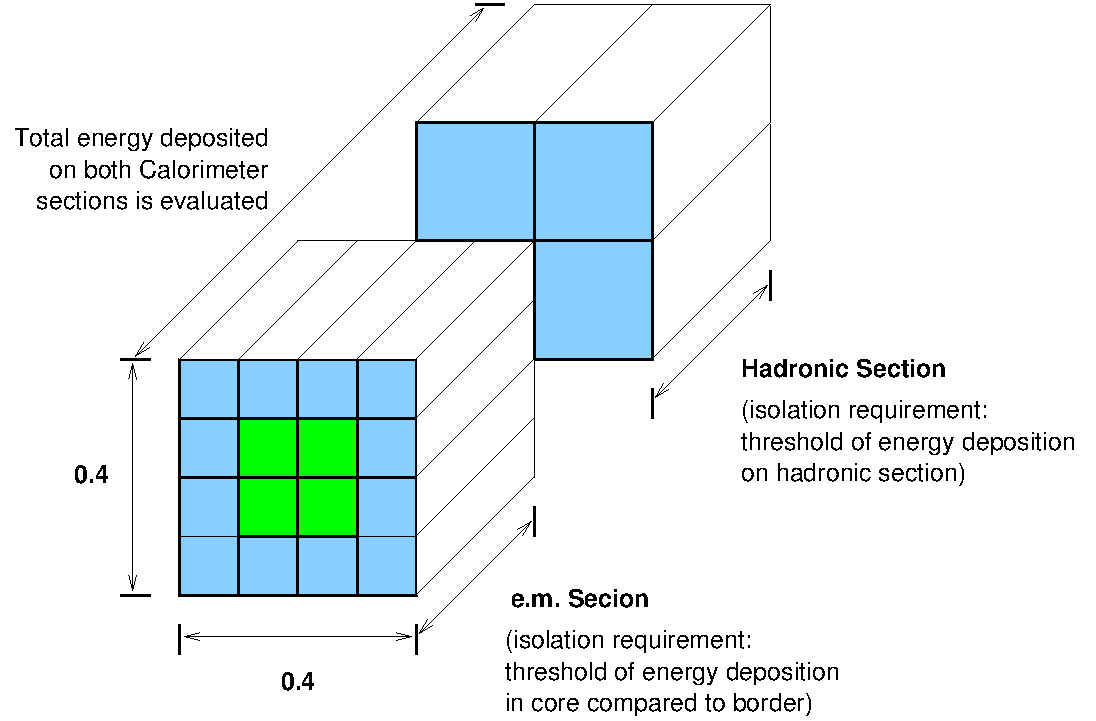
\includegraphics[scale=0.78]{l1-calo}
\end{center}
\caption{Representação gráfica do algoritmo de deteção de objetos e.m. no LVL1.}
\label{fig:l1-calo}
\end{figure}

Os diversos sub-módulos do LVL1 irão detetar e pré-classificar os elementos de
interesse para jatos, múons e energia faltante. Em seguida:

\begin{enumerate}
\item Os objetos detetados e seus pontos \textbf{centrais} de impacto
estimados no plano $\eta\times\phi$, ou seja, as RoIs, são encaminhados ao
Processador Central do Sistema de Filtragem do LVL1 (do inglês \eng{Central
Trigger Processor}, CTP) e uma decisão é feita levando-se em consideração as
assinaturas de interesse e resultados dos processamentos de outros módulos
(jatos, energia faltante e múons). A decisão de aprovar um evento é tomada
baseando-se em RoI's de acordo com critérios de preferência estipulados \eng{a
priori}. As RoI's que são utilizadas para a decisão de aprovação são rotuladas
``primárias'' ao passo que as demais, ``secundárias'';

\item Um sumário do resultado e das RoI's encontradas, já rotuladas (primárias
e secundárias) é repassado, através do \eng{RoI Builder} ao LVL2.
\end{enumerate}

A primeira vez onde o evento será analisado tendo por base a granularidade
máxima do detetor é no Segundo Nível de Filtragem do experimento ATLAS. O
objetivo deste nível de filtragem, de uma forma geral, é a confirmação das
informações do LVL1 e eventual depuração e extensão. Aproveitando-se de toda a
granularidade disponibilizada pelo sistema de leitura do detetor, o LVL2
começa analisando o evento através das RoI's classificadas como primárias pelo
LVL1.

Ao receber as informações das RoI's o \eng{Steering} ativará o passo de
decodificação do resultado do LVL1 e, em seguida, selecionará a próxima fase
de análise, que dependerá diretamente do tipo das RoI's primárias do
evento. No caso de RoI's do tipo e.m., um algoritmo de deteção de elétrons (e
fótons) será ativado.

\section{Deteção de elétrons no LVL2 do ATLAS}
\label{sec:classic-detection}

Como discutido anteriormente, na Seção~\ref{sec:e-detection}, o processo de
deteção veloz baseado em calorimetria pode ser sub-dividido nas seguintes partes:

\begin{enumerate}
\item Compactação do sinal de entrada;
\item Deteção da Física de interesse baseada no espaço comprimido.
\end{enumerate}

Para o ATLAS, a fase de compactação irá mapear o espaço de entrada definido
pelas células da RoI sendo tratada em 4 variáveis com alto poder
discriminatório, baseado na percepção da Física de interesse e da contaminação
esperada. No caso de elétrons, espera-se que haja forte contaminação de jatos
com muitas componentes e.m.. Desta forma, a compactação da informação de entrada
tentará realçar informações como a dispersão do objeto na RoI ou a
profundidade de interação do objeto com as diversas camadas do detetor.

O nome do algoritmo usado para a FEx de RoI's primárias tipo e.m. é
\emph{T2Calo}, uma abreviação composta das palavras \eng{Trigger}, LVL2 e
Calorimetria. As variáveis extraídas do \eng{cluster} definido pela RoI do
LVL1, por este algoritmo, estão descritas a seguir. Cada uma destas variáveis
define uma etapa ou mais etapas do processamento do T2Calo que está
esquematizada nas figuras correspondentes:

\begin{enumerate}
\item \textbf{Energia do núcleo e.m.}, Figura~\ref{fig:t2calo-1}: O
primeiro passo do algoritmo é um refinamento do centro da RoI. Isto é feito
encontrando-se o pico de deposi\-ção ener\-gé\-tica na segunda camada da
se\-ção eletroma\-gné\-tica do calo\-rí\-metro, que é tam\-bém a mais profunda
desta se\-ção (veja uma discus\-são mais detalhada da geometria do detetor na
Seção~\ref{sec:atlas-calo}). O valor do centro da cé\-lula é tomado como uma
nova estimativa de posicionamento da RoI e será utilizado para os cál\-culos
seguintes.

Em seguida, ainda utilizando-se dos dados da segunda camada e.m., calcula-se a
soma dos valores de deposição energética numa região de tamanho
$\Delta_\eta=0,075\times\Delta_\phi=0,175$ e numa região de tamanho
$\Delta_\eta=0,175\times\Delta_\phi=0,175$, ao redor do centro de impacto
encontrado anteriormente. De posse destes valores, a primeira característica
será extraída:

\begin{equation}
\rcore \text{ ou } R_\text{core} = \frac{\text{Energia}^{e.m.2}_{\Delta_\eta=0,075\times\Delta_\phi=0,175}}{\text{Energia}^{e.m.2}_{\Delta_\eta=0,175\times\Delta_\phi=0,175}}
\end{equation}

Esta quantidade tenta estimar o espalhamento da cascata formada pelo
decaimento do objeto na RoI. No caso do objeto ser um jato, espera-se que a
cascata tenha um espalhamento maior que no caso de elétrons, resultando em um
valor menor que 1 para esta quantidade;

\begin{figure}
\begin{center}
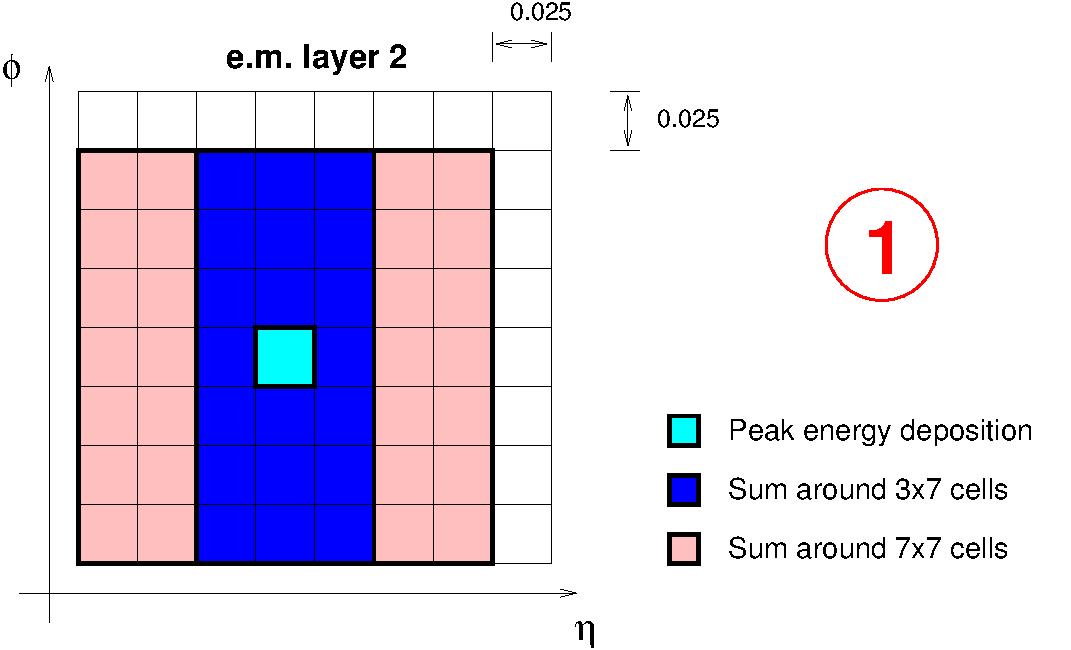
\includegraphics[scale=0.725]{t2calo-1}
\end{center}
\caption{T2Calo, Etapa 1: Cálculo do centro refinado e deposições de
energia na segunda camada e.m., para regiões de tamanho
$\Delta_\eta=0,075\times\Delta_\phi=0,175$ e
$\Delta_\eta=0,175\times\Delta_\phi=0,175$.} 
\label{fig:t2calo-1}
\end{figure}

\item \textbf{Máximos na primeira camada e.m.}, Figura~\ref{fig:t2calo-2}: Os
dois maiores picos de energia na primeira camada da seção e.m. (denominados
$E_1$ e $E_2$ respectivamente) são detetados. De posse destes valores, a
segunda característica é extraída:

\begin{equation}
\eratio \text{ ou } E_\text{ratio} = \frac{E_1-E_2}{E_1+E_2}
\end{equation}

Uma vez que jatos de par\-tí\-culas interagem de forma mais espalhada do que
e\-lé\-trons, espera-se que, na primeira camada e.m., sejam observados vários
picos. Desta forma, se o objeto for um elétron (objeto único), espera-se que
$E_2=0$, já que a cascata de partículas que o elétron forma na sua interação
com o calorímetro é, tipicamente, bastante estreita. Assim sendo, para
elétrons, \eratio tenderá a 1. Para jatos, normalmente, \eratio\ será menor
que 1, já que $E_2 \neq 0$.

\begin{figure}
\begin{center}
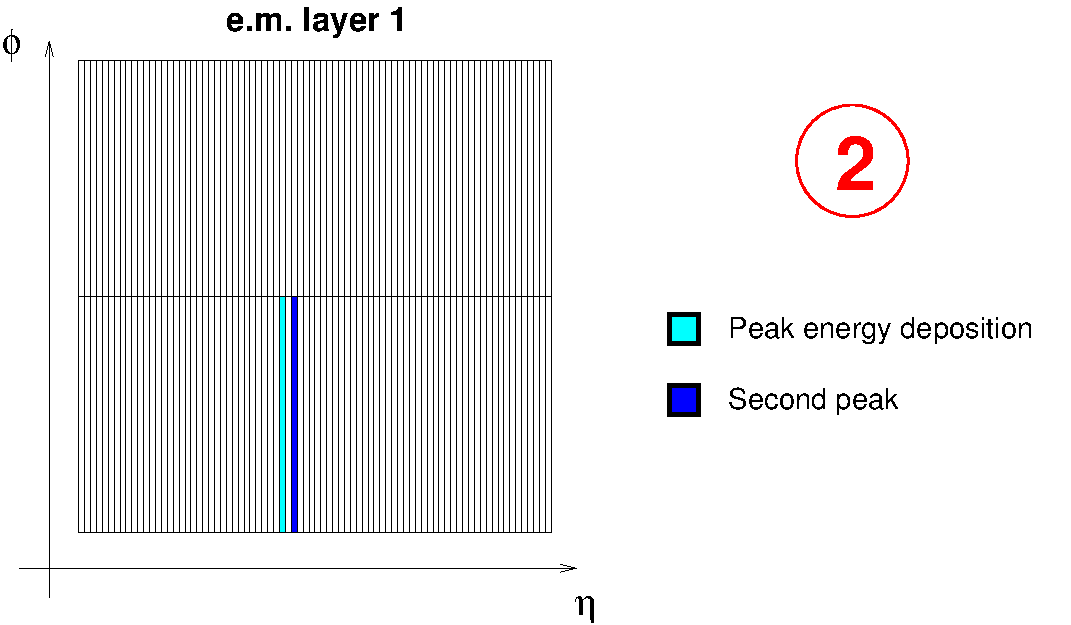
\includegraphics[scale=0.8]{t2calo-2}
\end{center}
\caption{T2Calo, Etapa 2: Procura dos dois maiores picos na primeira camada e.m..}
\label{fig:t2calo-2}
\end{figure}

\item \textbf{Energia e.m.}, Figura~\ref{fig:t2calo-3}: Os valores parciais de
deposição energética para cada camada da seção e.m., numa região de
$\Delta_\eta=0,075\times\Delta_\phi=0,175$ ao redor do pico de deposição
energética na segunda camada, também são calculados. Destas somas parciais, a
terceira característica da RoI é calculada somando-se estes 4 valores. O valor
original calculado é dividido pelo $\cosh{|\eta|}$ para que obtenha-se a
energia transversa\footnote{O termo ``transverso'' neste contexto refere-se ao
feixe de partículas.} (projetada no plano $x \times y$ do detetor). Espera-se
que a energia de elétrons esteja totalmente contida nesta janela; por sua vez,
jatos devem apresentar uma fração menor de sua energia depositada nesta área;

\begin{figure}
\begin{center}
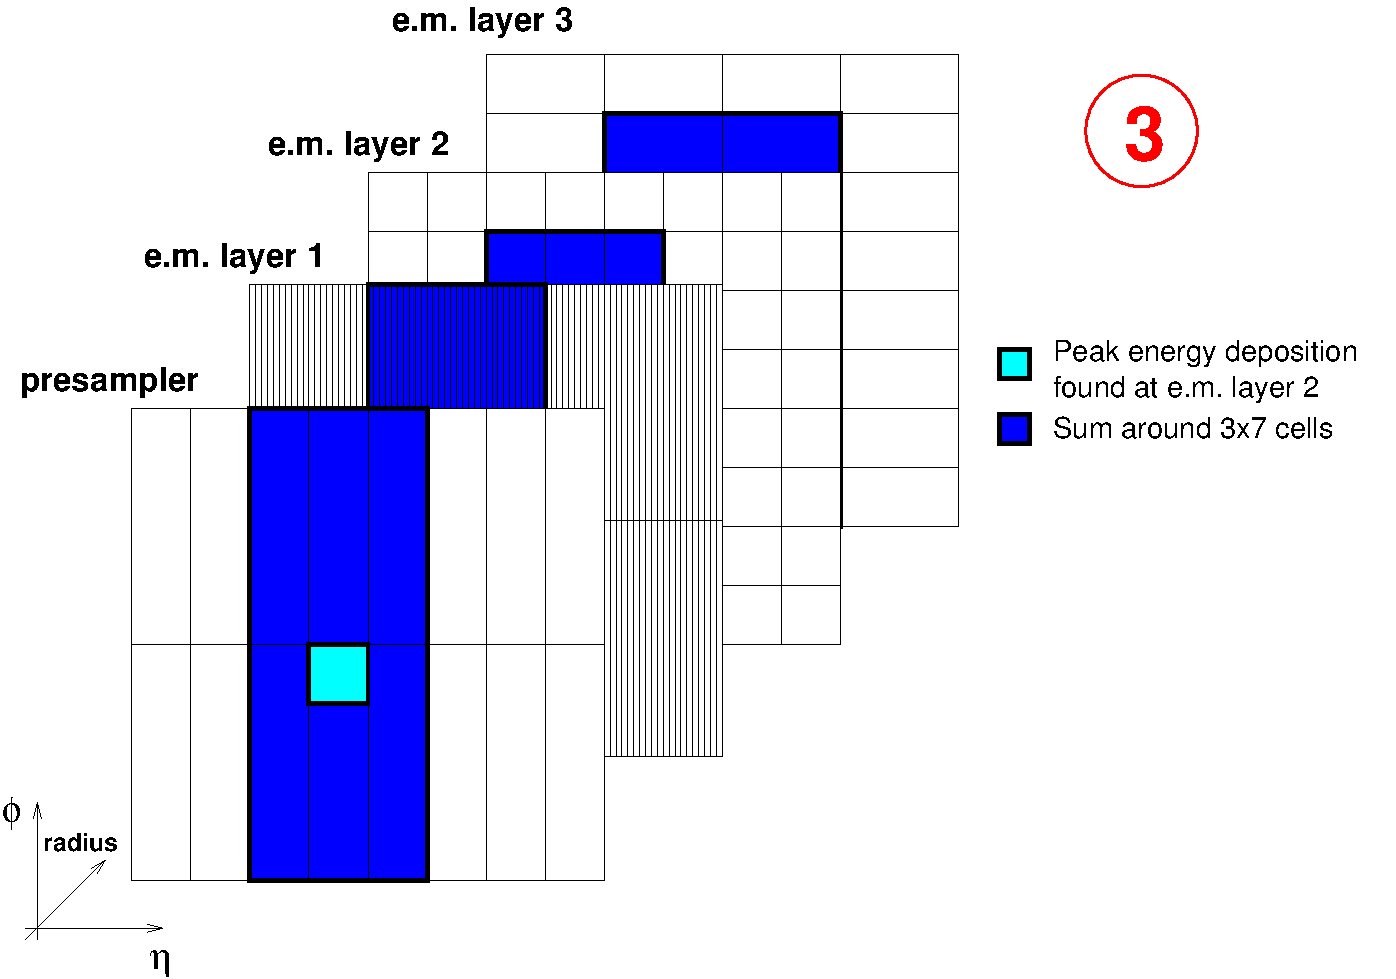
\includegraphics[scale=0.55]{t2calo-3}
\end{center}
\caption{T2Calo, Etapa 3: Cálculo dos somatórios parciais de energia por
camada, em uma área equivalente a $\Delta_\eta=0,075\times\Delta_\phi=0,175$.}
\label{fig:t2calo-3}
\end{figure}

\item \textbf{$\text{Energia
Hadrônica}_{\Delta_\eta=0,2\times\Delta_\phi=0,2}$}: Calcula-se a energia
total numa região $\Delta_\eta=0,2\times\Delta_\phi=0,2$, centrado no pico de
deposição energética na segunda camada e.m.. Este procedimento é executado
para cada camada na seção hadrônica, e depois uma somatório do total
transverso é executado. Para elétrons, a quantidade de energia depositada na
camada hadrônica deve ser próxima de zero, enquanto que, para jatos, espera-se
que seja diferente de zero.

\begin{figure}
\begin{center}
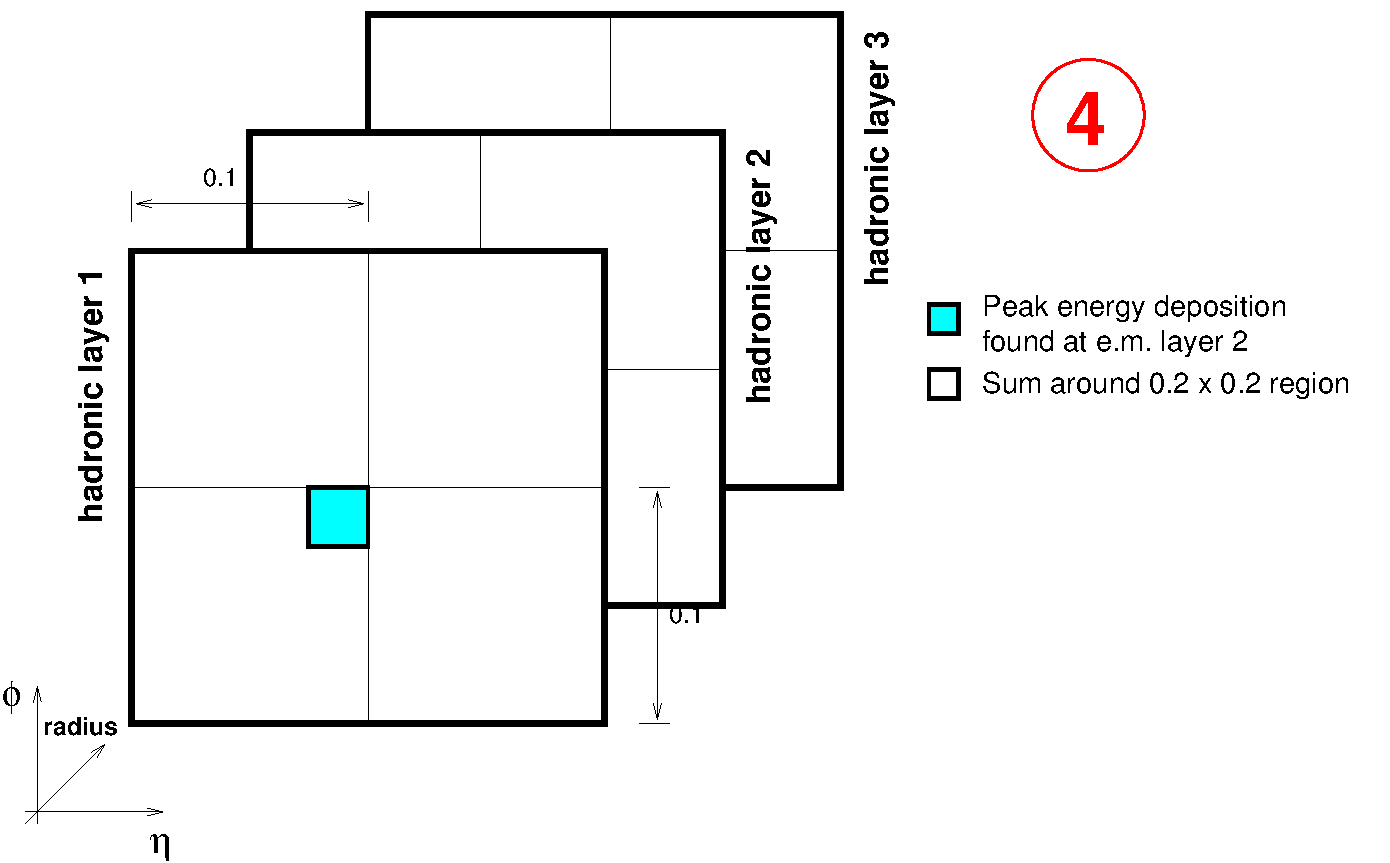
\includegraphics[scale=0.6]{t2calo-4}
\end{center}
\caption{T2Calo, Etapa 4: Valores parciais e somatório das energias, em uma
área equivalente a $0,2\times0,2$ no plano $\eta\times\phi$, para as camadas
da seção hadrônica.} 
\label{fig:t2calo-4}
\end{figure}

\end{enumerate}

O algoritmo de deteção propriamente dito segue a execução do T2Calo e é
chamado \emph{EGammaHypo}. Este algoritmo tem a função exclusiva de combinar
as informações disponibilizadas a partir do processo de extração de
características e tomar uma decisão simples baseada nas propriedades físicas
das partículas de interesse. A seqüência discriminatória empregada pelo
EGammaHypo está representada a seguir, em pseudo-código: 

\newcommand{\textbu}[1]{\textbf{\underline{#1}}}
\newcommand{\IF}[1]{\textbu{se} #1, \textbu{então}}
\newcommand{\RETURN}[1]{\\ \textbu{retornar} #1\textbf{;}}
\newcommand{\lumihi}{\ensuremath{10^{33} \text{cm}^{-2}\text{s}^{-1}}}

\begin{description}
\item[\ding{182}] \IF{$\rcore \lessapprox \text{corte}_{\rcore}$}
	\RETURN{\textbf{não é} elétron}

\item[\ding{183}] \IF{$\eratio \lessapprox \text{corte}_{\eratio}$}
	\RETURN{\textbf{não é} elétron}

\item[\ding{184}] \IF{$\etem \lessapprox \text{corte}_{\etem}$}
	\RETURN{\textbf{não é} elétron}

\item[\ding{185}] \IF{$\ethad \gtrapprox \text{corte}_{\ethad}$}
	\RETURN{\textbf{não é} elétron}

\end{description}

Se o objeto definido pelo LVL1 conseguir passar todos os critérios definidos
neste procedimento, é promovido a ``candidato à elétron'' dentro do LVL2. As
fases seguintes de discriminação tentarão encontrar um traço, com momento
equivalente a energia do \eng{cluster}, e uma nova rodada de hipóteses
confirmará (ou não) o possível elétron. A procura de traços nos detetores
internos é um procedimento tipicamente lento (na ordem de dezenas, dependendo
centenas de milissegundos \cite{hlt-tdr}), e deve ser evitada tanto quanto
possível. Por outro lado, deseja-se que o sistema de deteção preliminar,
baseado em calorimetria, seja o mais rápido possível, e mantenha bons níveis
de discriminação, como já discutido.

Uma das estratégias em consideração atualmente, pondera sobre a utilização dos
diversos estágios de hipótese de forma seqüencial, durante a extração de
característica. Neste caso, após interagir com a segunda camada e.m., o T2Calo
seria brevemente suspenso e a primeira das hipóteses verificada, criando
recursos para uma rejeição mais antecipada. Em seguida, os dados da RoI para a
primeira camada e.m. seriam carregados no processador, a segunda variável
seria calculada e mais uma rodada de decisão seria tomada. As próximas etapas
seriam a carga dos dados da terceira camada e.m. e do pré-irradiador,
seguindo-se da análise de dados na seção hadrônica.

\subsection{Ajuste fino para cada canal}

Para cada uma das assinaturas de interesse aprovadas pelo LVL1, o segundo
nível contará com algoritmos e sistemas de hipótese adequados àquela Física. É
interessante notar que, mesmo para os canais similares, e.g. (veja a
Tabela~\ref{tab:l1-rates}) \texttt{EM25i} e \texttt{EM15i}, os cortes impostos
pelo algoritmo de hipótese serão otimizados para estas categorias de energia.

%Neste trabalho estaremos comparando os diversos algoritmos de deteção
%utilizando um conjunto de eventos destinado ao estudo da discriminação
%elétron/jato no contexto da assinatura mais freqüente do experimento:
%\texttt{EM25i}.

\section{Caracterização do T2Calo e do EGammaHypo}
\label{sec:def-eghypo}

Para a caracterização de operação do T2Calo e do algoritmo de hipótese
associado, o EGammaHypo, os seguintes grupamentos de dados foram
considerados:

\begin{itemize}
\item Cerca de 23.000 elétrons simulados via Monte Carlo para o \eng{Data
Challenge} 1, no CERN, proveniente de interações tipo $H (130
\text{GeV})\rightarrow ZZ
\rightarrow 4e^-$ e $H (130 \text{GeV})\rightarrow ZZ \rightarrow 2e^- +
2\mu$. Os elétrons de cada evento simulado interagem com diferentes regiões do
detetor;
\item Cerca de 250.000 jatos-duplos, simulados via Monte Carlo (\eng{Pythia})
para o \eng{Data Challenge} 1, no CERN, com energia total, fixa em 25 GeV,
também interagindo com várias partes do detetor.
\end{itemize}

Nos dois casos, considerou-se simulações com ruído, proveniente da eletrônica,
e uma planta de detetor compatível com o que está sendo instalado atualmente
na caverna do experimento, provendo um ambiente bastante acurado dentro do que
é possível prever-se em termos de operação, mas ainda exeqüível para um
ambiente de simulação.

Esta massa original de dados foi submetida a uma simulação do LVL1, que
implementa o algoritmo discutido na Seção~\ref{sec:lvl2-detect-electron},
aceitando todos os eventos com objetos tipo EM com as seguintes
características:

\begin{itemize}
\item ao menos 10 GeV numa região de $2\times2$ torres de filtragem na seção
e.m.;
\item no máximo 4 GeV na região periférica ao núcleo de $2\times2$ torres de
filtragem; 
\item no máximo 2 GeV de depósito na seção hadrônica;
\item qualquer valor para o centro em $\phi$;
\item $\eta$ variando de $-2,5$ a $+2,5$;
\end{itemize}

Um total de cerca de 22.000 elétrons e 7.000 fazem parte da massa de dados
remanescente após a aplicação dos cortes acima. A
Figura~\ref{fig:transverse-energy} contém os histogramas de deposição
energética total transversa de elétrons e jatos, em uma janela de $0,4 \times
0,4$ no plano $\eta\times\phi$, considerando-se as duas seções do calorímetro
(e.m. e hadrônica). É possível distinguir um corte acentuado nas redondezas de
aproximadamente 10~GeV, que equivale à ação da simulação do LVL1, como
esperado. Para o histograma de jatos a média aproxima-se ao valor esperado de
25~GeV, exibindo um pico pronunciado ao redor deste valor. Como observa-se,
grande parte dos jatos encontram-se com valor de energia transversa entre 10 e
40~GeV, enquanto que para elétrons, a distribuição decai suavemente até
$\approx$ 91~GeV (aproximadamente a massa de repouso do bóson Z).
%Antes do corte, é possível distinguir uma cauda, se estendendo até a
%origem. Este fenômeno pode ser observado no LVL2 já que os valores de
%calibração de energia aplicados às células do calorímetro neste nível de
%filtragem não estão disponíveis ao nível de filtragem anterior.

% Interessante observar que isto poderá e deverá influenciar nos resultados
% disponíveis, mas o que deseja-se demonstrar é a técnica e não uma solução
% pronta para o problema.

\begin{figure}
\begin{center}
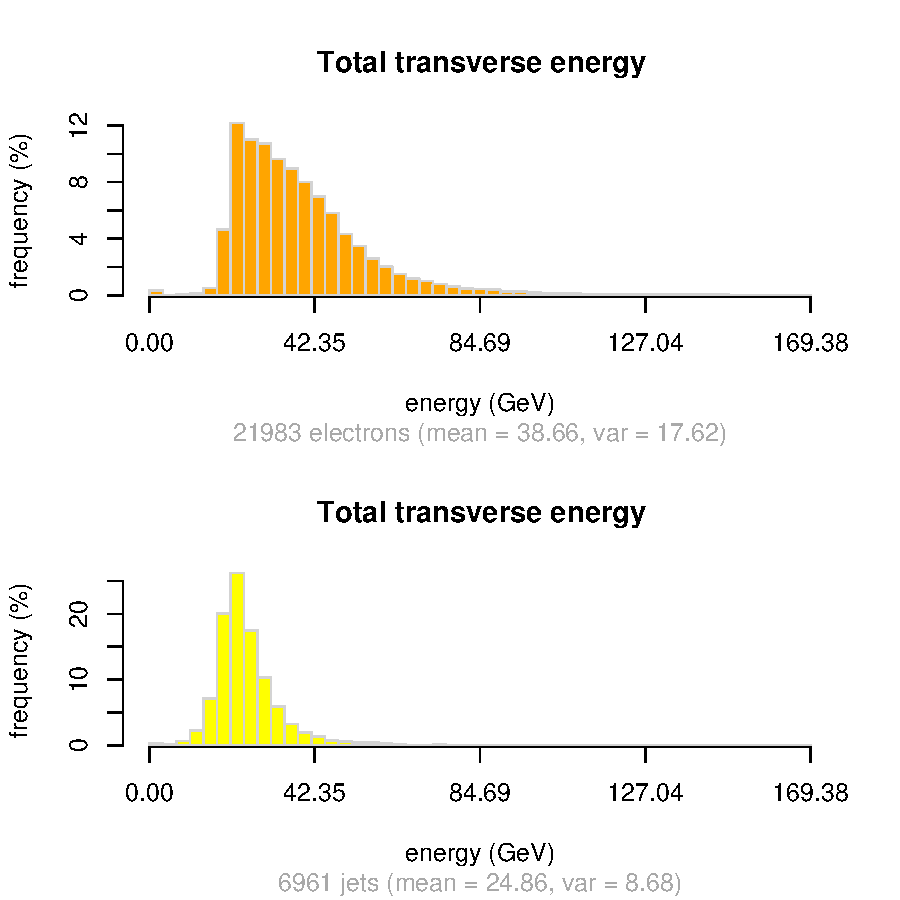
\includegraphics[scale=0.95]{transverse-energy}
\end{center}
\caption{A deposição total de energia em uma região $0,4 \times 0,4$ no plano
$\eta\times\phi$ para elétrons (em cima) e jatos (em baixo) para a massa de
dados disponível para o estudo.}
\label{fig:transverse-energy}
\end{figure}

As Figuras~\ref{fig:em-tenergy} e \ref{fig:had-tenergy} mostram histogramas da
energia transversa total por seção de calorimetria para e\-lé\-trons e
jatos. Nota-se que, para elétrons, quase 100\% da energia total do objeto é
retida na seção e.m., enquanto que, para jatos, observa-se algum vazamento de
energia na seção hadrônica. Embora o corte realizado pelo LVL1 tenha sido em
2~GeV para o vazamento de energia nesta seção, observa-se uma quantidade não
desprezível de eventos com energia hadrônica além deste valor. Por outro lado,
a energia total nesta seção decai rapidamente e assume-se que a existência
desta cauda esteja relacionada à (baixa) qualidade da calibração dos dados
utilizada no LVL1.

\begin{figure}
\begin{center}
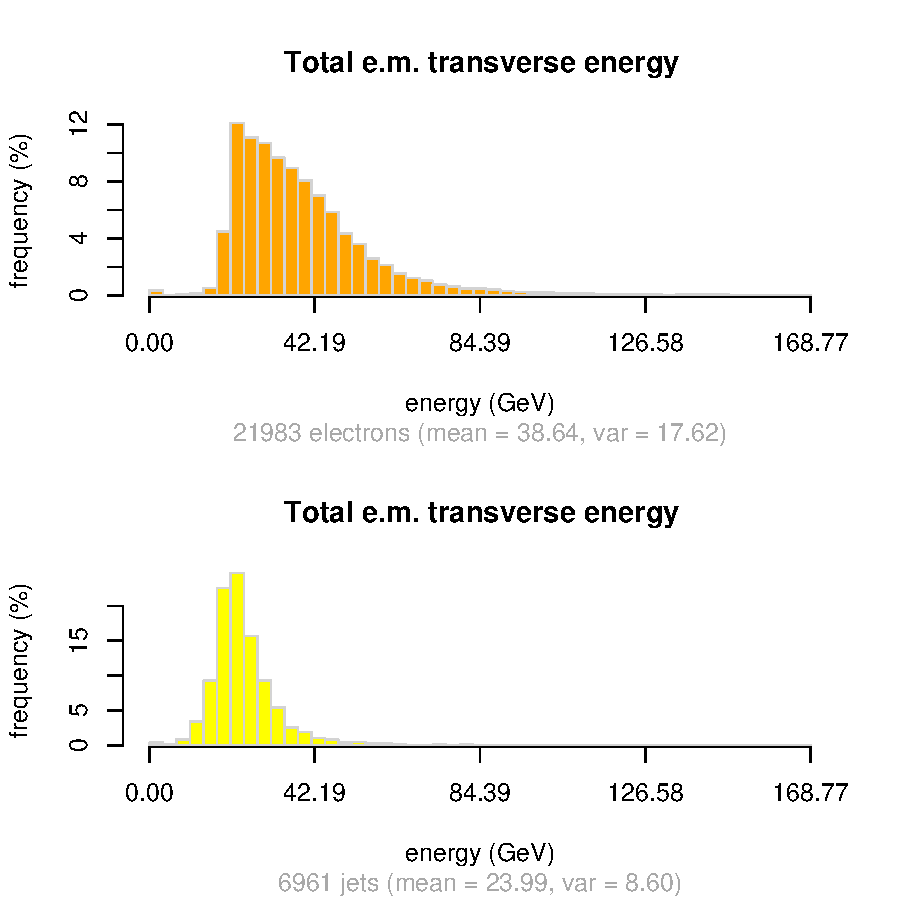
\includegraphics[scale=0.95]{em-tenergy}
\end{center}
\caption{A deposição total de energia na seção e.m. em uma região $0,4 \times
0,4$ no plano $\eta\times\phi$ para elétrons (em cima) e jatos (em baixo) para
a massa de dados disponível para o estudo. As contagens estão normalizadas.}
\label{fig:em-tenergy}
\end{figure}

\begin{figure}
\begin{center}
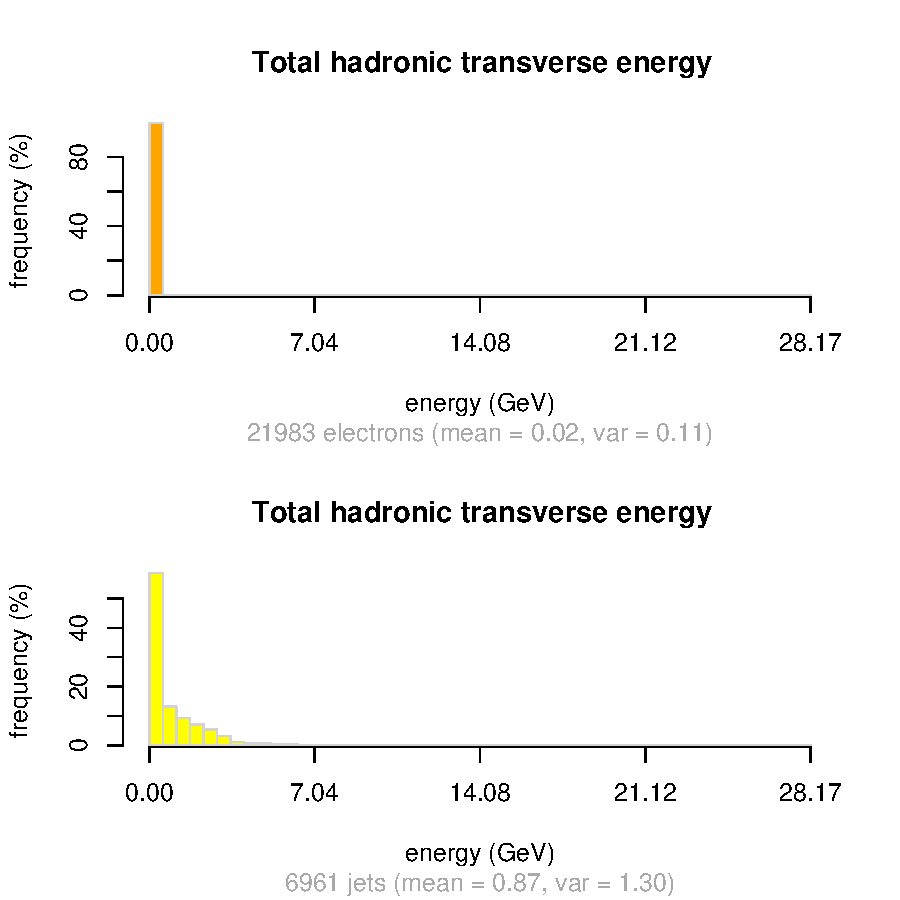
\includegraphics[scale=0.95]{had-tenergy}
\end{center}
\caption{A deposição total de energia na seção hadrônica em uma região $0,4 \times
0,4$ no plano $\eta\times\phi$ para elétrons (em cima) e jatos (em baixo) para
a massa de dados disponível para o estudo. As contagens estão normalizadas.}
\label{fig:had-tenergy}
\end{figure}

As Figuras~\ref{fig:rcore} e \ref{fig:eratio} mostram, respectivamente, a
fração \rcore e \eratio, tal como utilizada pelo EGammaHypo para definir a
eficiência de deteção de elétrons e jatos. Na Figura~\ref{fig:rcore},
observa-se que a distribuição para elétrons tem média bastante próxima a 1 e
baixíssima variância. Para jatos, a média é mais baixa e a distribuição
apresenta longa cauda em direção à origem. No caso da variável \eratio, que
tem por objetivo detetar picos de deposição energética na primeira camada
e.m., para elétrons observa-se um pico dominante em 1, ao passo que, para
jatos, há uma distribuição mais uniforme, indicando uma separabilidade
linear.

\begin{figure}
\begin{center}
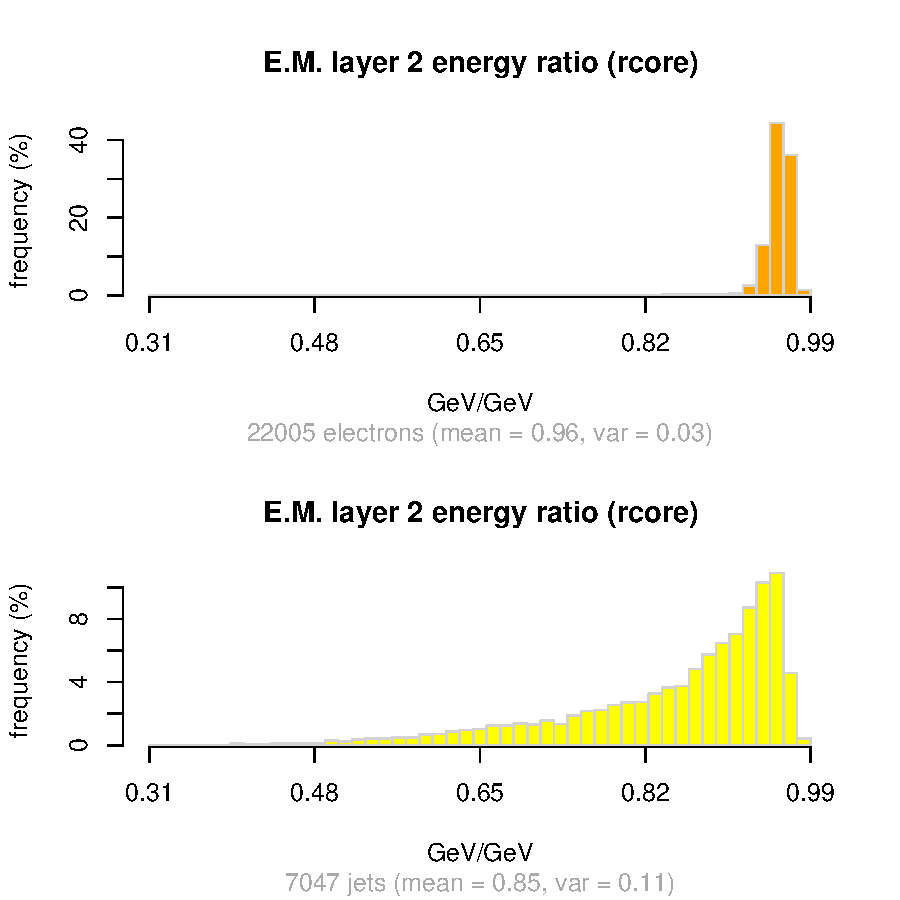
\includegraphics[scale=0.95]{rcore}
\end{center}
\caption{Distribuição da variável \rcore para elétrons (em cima) e jatos
(embaixo). As contagens estão normalizadas.}
\label{fig:rcore}
\end{figure}

\begin{figure}
\begin{center}
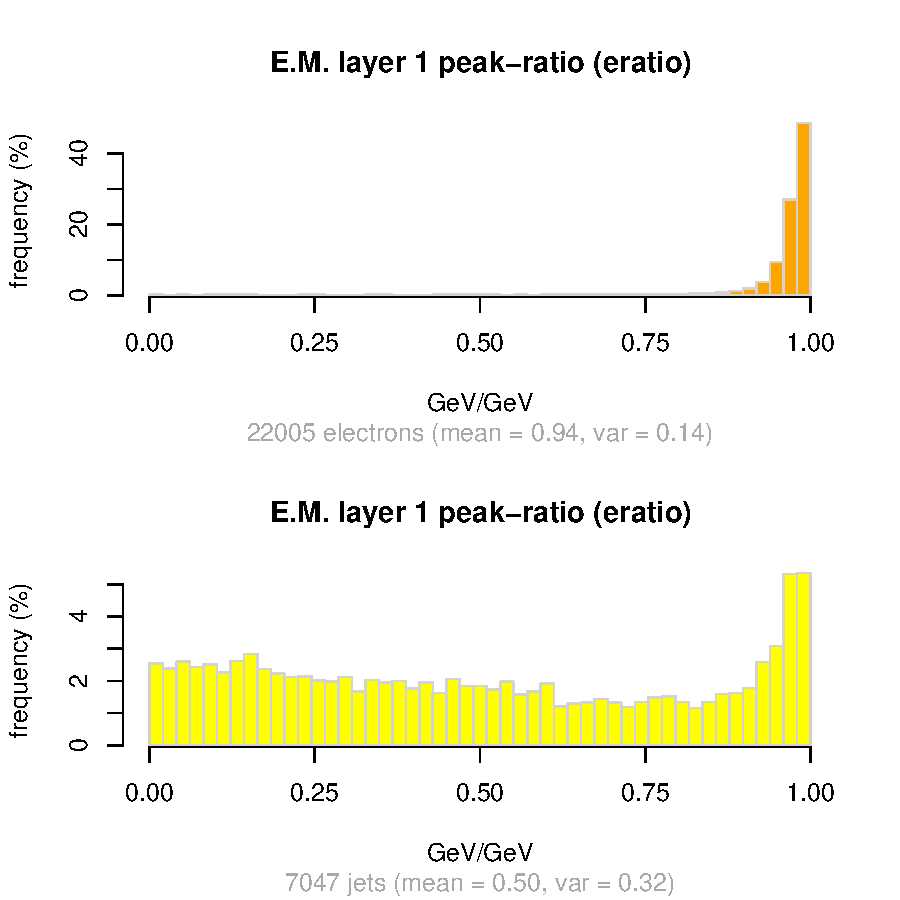
\includegraphics[scale=0.95]{eratio}
\end{center}
\caption{Distribuição da variável \eratio para elétrons (em cima) e jatos
(embaixo). As contagens estão normalizadas.}
\label{fig:eratio}
\end{figure}

As Figuras~\ref{fig:eta} e \ref{fig:phi} mostram histogramas para elétrons e
jatos dos centros refinados pelo T2Calo das RoI's em questão, tanto em relação
à variável $\eta$ quanto à variável $\phi$. É possível distinguir uma
uniformidade na distribuição em $\phi$ e uma tendência a concentração de
eventos nas proximidades de $\eta=0$, como é aguardado no experimento.

\begin{figure}
\begin{center}
\includegraphics[scale=0.95]{eta}
\end{center}
\caption{Distribuição em $\eta$ dos centros refinados das RoI's para elétrons
(em cima) e jatos (embaixo). As contagens estão normalizadas.}
\label{fig:eta}
\end{figure}

\begin{figure}
\begin{center}
\includegraphics[scale=0.95]{phi}
\end{center}
\caption{Distribuição em $\phi$ dos centros refinados das RoI's para elétrons
(em cima) e jatos (embaixo). As contagens estão normalizadas.}
\label{fig:phi}
\end{figure}

Exceto por eventuais problemas na lógica de simulação (Monte Carlo) e
filtragem (pelo LVL1), estima-se que a massa de dados seja representativa do
problema da separação entre jatos e elétrons. Deve ser levado em consideração
que, para jatos, o pico ao redor de 25~GeV poderá introduzir imprecisões na
definição da capacidade de deteção de elétrons bastante energéticos, presentes
na massa de estudo. Sempre que possível, tentar-se-á levar estas restrições em
consideração.

\subsection{Deteção de elétrons com o EGammaHypo e sua otimização}
\label{sec:eghypo}

Para que a eficiência de deteção do algoritmo proposto pelo EGammaHypo seja
estimada, deve-se passar a massa de dados de estudo por um processo de
otimização que ajude o especialista a selecionar os patamares de corte que
definem o algoritmo, como exposto na Seção~\ref{sec:classic-detection}. Para
tal, dividiu-se o conjunto de dados em 2 metades com aproximadamente o mesmo
número de RoI's. A primeira metade será utilizada para o ``treinamento'' ou
otimização dos cortes, enquanto que a segunda será utilizada para o teste dos
cortes de forma que seja possível testar se, para uma massa de dados jamais
apresentada ao sistema, a eficiência de deteção está de acordo com aquela
encontrada durante a determinação dos cortes. Desta forma, saberemos se o
detetor está demasiado especializado nos dados presentes no conjunto de
treinamento ou pode ser utilizado \emph{genericamente} para a deteção de
elétrons e jatos.

O algoritmo de otimização não será exaustivo, varrendo todo o espaço de dados,
mas partirá de patamares pré-fixados em valores intuitivos e definirá uma
sub-área de variação por onde testará exaustivamente as combinações dos 4
cortes necessários, como é normalmente feito atualmente. Eis aqui os patamares
e passos de busca (ou \emph{possibilidades}) que utilizaremos:

\begin{enumerate}
\item Corte em \rcore: de 0,6 a 1,0, em passos de 0,01 (41 possibilidades);
\item Corte em \eratio: de 0,6 a 1,0, em passos de 0,01 (41 possibilidades);
\item Corte em \etem: de 5000 a 30000 MeV em passos de 500 MeV (51
possibilidades);
\item Corte em \ethad: de 0 a 4000 MeV em passos de 500 MeV (9
possibilidades). 
\end{enumerate}

Para cada corte, a totalidade da massa de dados de treinamento do método é
avaliada e as RoI's que \textit{sobrevivem} ao corte são levadas à próxima
etapa. As eficiências relativas e a quantidade de dados utilizadas para o
teste da fase seguinte são acumulados para posterior análise. Levando-se em
consideração o número de combinações dadas as possibilidades do problema de
otimização e considerando-se que a superfície de erro não possua um único
mínimo, há de se tentar $41 \times 41 \times 51 \times 9 = 771579$ diferentes
combinações, neste caso, antes de qualquer conclusão.

Está claro que uma varredura completa do espaço de parâmetros,
i.e. buscando-se todo o espaço de possibilidades ao invés dos sub-conjunto
utilizados, estaria fora de questão para uma utilização em condições que
possam variar em questão de horas, como é o caso do experimento ATLAS. Desta
forma, seria necessária uma antecipação para os cortes ou uma redução do
espaço de busca, permitindo uma otimização mais rápida. A utilização de
programas especialmente codificados para a tarefa também poderia diminuir o
tempo de teste, tornando o método mais atraente para uma utilização prática.

A Figura~\ref{fig:eghypo-best-sp-train} mostra os resultados da busca
exaustiva definida anteriormente. Esta figura de mérito, normalmente chamada
de \textit{Característica de Operação do Receptor} (do inglês,
\eng{Receiver Operating Characteristics}, ROC \cite{vantrees}), contém os
resultados de cada ponto de operação do algoritmo EGammaHypo. O eixo vertical
denota a eficiência na deteção do sinal de interesse (elétrons), enquanto o
eixo horizontal, a taxa de falso-alarme (erro em jatos) naquele ponto de
operação. A taxa de falso alarme é escalonada em 25~kHz, que é a taxa máxima
de ruído de fundo esperada. O valor do eixo horizontal portanto, denota a
quantidade de jatos que serão aprovados pelo LVL2, como elétrons e, portanto,
representa uma medida direta da taxa de eventos descarregados no Filtro de
Eventos.

Observa-se que, para o conjunto de intervalos testado, a massa de resultados
assume uma forma angular. Ao redor do ponto de flexão, na parte exterior da
massa de resultados, encontraremos as melhores relações de eficiência
\textit{versus} falso-alarme para este discriminador. O ponto destacado nesta
figura representa o conjunto de cortes que maximiza a multiplicação da soma
das eficiências de deteção pelo produto entre elas, ou seja:

\begin{equation}
SP = (\text{efic.}_{classe_1} + \text{efic.}_{classe_2}) \times
(\text{efic.}_{classe_1} \times \text{efic.}_{classe_2})
\label{eq:sp-product}
\end{equation}

O produto SP de um detetor para 2 classes de eventos apresenta um máximo
($=2,0$) quando a eficiência na deteção de ambas as classes é máximo
(i.e. $=1,0$), e um mínimo em $0$ quando a eficiência de deteção de
\textbf{qualquer} uma das duas classes de eventos é $0$. É interessante notar
que, para um determinado classificador, o valor do máximo da
Equação~\ref{eq:sp-product} indicará o ponto de inflexão da curva R.O.C.. Este
ponto determina a melhor relação de deteção entre as duas classes de eventos
para o classificador.

À medida que a curva R.O.C. se aproxima, em detrimento de uma melhora na
eficiência de deteção, do eixo vertical para $\text{Prob.}_\text{falso-alarme}
= 0$ e do eixo horizontal para $\text{Prob.}_\text{deteção} = 1,0$, o máximo
da Equação~\ref{eq:sp-product} aumentará. Por esta razão utilizar-se-á o valor
máximo produto SP de um detetor como uma figura de mérito de sua eficiência de
classificação.

No caso específico em análise, o ponto onde produto SP atinge seu máximo
determina uma eficiência de deteção de elétrons de 91,85\% contra 10,19\% de
falso alarme na deteção de jatos, ou 2,55 kHz, levando-se em consideração a
contaminação do canal de elétrons na saída do LVL1. O valor do produto SP no
ponto em questão é de $1,50$.

\begin{figure}
\begin{center}
\includegraphics[scale=0.98]{eghypo/eghypo-best-sp-train}
\end{center}
\caption{A curva ROC para 771.579 combinações de valores de corte para o
algoritmo EGammaHypo.}
\label{fig:eghypo-best-sp-train}
\end{figure}

Os seguintes valores de corte determinam o detetor marcado na
Figura~\ref{fig:eghypo-best-sp-train}:
\begin{enumerate}
\item \rcore: 0,93;
\item \eratio: 0,82;
\item \etem: 14.500 MeV;
\item \ethad: 500 MeV.
\end{enumerate}

Aplicando-se estes cortes ao conjunto de teste, de forma análoga, obtém-se
91,62 \% de eficiência na deteção de elétrons contra 10,45 \% de falso-alarme
($SP = 1,49$). Este resultado indica também que os dois sub-conjuntos de dados
(treino e teste) são estatisticamente semelhantes. Durante a busca exaustiva
deste resultado, acumularam-se os resultados de eficiência e falso-alarme
parciais entre operações de corte. Estes valores podem ser vistos na
Tabela~\ref{tab:eghypo-partials}. Como é possível avaliar, a partir desta
tabela, as variáveis \rcore e \eratio são as mais discriminatórias, deixando
passar apenas cerca de 30 \% e 45 \% dos jatos avaliados, respectivamente. O
corte em \etem não reduz a taxa de eventos, sendo praticamente irrelevante a
este processo de discriminação. Este comportamento é esperado, para a massa de
dados sendo avaliada, uma vez que os jatos disponíveis tem energia fixa em 25
GeV e que elétrons estão espalhados no espectro de energia. O vazamento de
energia na seção hadrônica (último corte), ainda conseguirá diminuir a taxa de
falso-alarme na saída do detetor.

%% COMENTÁRIO: SERIA BOM DIZER PORQUE O CORTE EM EM_ET NÃO É TÃO RELEVANTE...
%% IDÉIAS: ALTA CORRELAÇÃO COM RCORE E ERATIO => PCA?

\begin{table}
\caption{Valores parciais de deteção e falso-alarme para o detetor baseado no
algoritmo EGammaHypo.}
\label{tab:eghypo-partials}
\begin{center}
\begin{tabular}{|l|l|r|r|}
\hline
\textbf{Ordem} & \textbf{Variável} & \textbf{Eficiência (\%)} &
\textbf{Falso-alarme (\%)} \\ \hline
1 & \rcore & 96,4 & 30,5 \\ \hline
2 & \eratio & 95,7 & 43,6 \\ \hline
3 & \etem & 99,9 & \textbf{98,9} \\ \hline
4 & \ethad & 91.8 & 77.4 \\ \hline
\end{tabular}
\end{center}
\end{table}

As Figuras~\ref{fig:eghypo-eta-scan-test}, \ref{fig:eghypo-phi-scan-test} e
\ref{fig:eghypo-emet-scan-test} mostram os valores parciais de eficiência e
falso-alarme considerando-se uma divisão dos dados por $\eta$, $\phi$ e por
energia total transversa na seção e.m. dos calorímetros. No caso da varredura
em $\eta$, é possível notar que a eficiência de deteção do método apresenta
uma queda abrupta próximo ao vão entre a seção do barril e da tampa ($\eta
\approx 1,5$), o que é esperado devido a ausência de elementos de deteção
nesta área. Para a varredura em $\phi$, observa-se uma distribuição bastante
homogênea para a eficiência de deteção de elétrons e jatos, apesar da baixa
estatística para jatos em alguns intervalos em $\phi$ (muitos canais possuem
apenas 30 a 40 jatos, como é possível observar na
Figura~\ref{fig:transverse-energy}). A varredura por \etem indica que o método
é bastante robusto na deteção de elétrons, aumentando sua eficiência
suavemente com o valor de energia da RoI. Este comportamento é esperado pois
sabe-se que a resolução em energia de um calorímetro aumenta com a energia do
objeto \cite{wigmans-book} e, portanto, a capacidade discriminante do
sistema. Por outro lado, jatos mais energéticos tendem a penetrar ainda mais
no calorímetro, fazendo com que a deteção de elétrons se torne mais fácil. O
falso-alarme em jatos também aumenta com a energia do objeto analisado, embora
seja difícil estimar com precisão a qualidade do valor de falso-alarme
determinado, uma vez que a estatística para jatos acima de 50 GeV é
praticamente inexistente.

\begin{figure}
\begin{center}
%\includegraphics[angle=90,width=15cm,height=20cm]{eghypo-eta-scan-test}
\includegraphics[scale=0.98]{eghypo/eghypo-eta-scan-test}
\end{center}
\caption{Eficiência de deteção contra falso-alarme por $\eta$ para o conjunto
de testes utilizando o algoritmo EGammaHypo.}
\label{fig:eghypo-eta-scan-test}
\end{figure}

\begin{figure}
\begin{center}
\includegraphics[scale=0.98]{eghypo/eghypo-phi-scan-test}
\end{center}
\caption{Eficiência de deteção contra falso-alarme por $\phi$ para o conjunto
de testes utilizando o algoritmo EGammaHypo.} 
\label{fig:eghypo-phi-scan-test}
\end{figure}

\begin{figure}
\begin{center}
\includegraphics[scale=0.98]{eghypo/eghypo-emet-scan-test}
\end{center}
\caption{Eficiência de deteção contra falso-alarme por \etem para o conjunto
de testes utilizando o algoritmo EGammaHypo.}
\label{fig:eghypo-emet-scan-test}
\end{figure}

%\subsection{Análise de Componentes Principais}

%Isto não é óbvio que melhorará a análise do método já que temos poucas
%variáveis a a informação contida nelas traz bastante informação, mas não
%informação discriminante.

%Levando-se em consideração os dados da Tabela~\ref{tab:eghypo-partials}, é
%possível intuir que exista uma grande correlação entre as 4 variáveis
%definidas pelo T2Calo e utilizados pelo EGammaHypo para a deteção de
%elétrons. A técnica de Análise de Componentes Principais \cite{vantrees}
%define uma transformação linear que, quando aplicada a massa de dados de onde
%é originalmente extraída, completamente a descorrelaciona. Esta transformada
%é comumente conhecida como KLT (do inglês \eng{Karhunen-Loève Transform}).

%Uma das técnicas para o cálculo da KLT utiliza a matriz de covariância C do
%conjunto de dados de analisados para calcular 

%\cite{vantrees}, é possível calcular a transformação , que
%completamente descorrelacionará os dados disponíveis. 

\typeout{ *************** End of file baseline.tex *************** }

%% Hello emacs, this is -*- latex -*-
\typeout{ ====================================================================}
\typeout{ This is file neural.tex, created at 27-Aug-2005 }
\typeout{ Maintained by Andre Anjos <Andre.dos.Anjos@cern.ch> }
\typeout{ ====================================================================}

\chapter{Análise multi-variável baseada em calorimetria para a deteção
elétron/jato} 
\label{chap:neural}

Neste capítulo, analisa-se o modelo de classificação elétron/jato proposto
atualmente no CERN e desenvolvem-se sistemas de classificação de simples
treinamento e emprego, baseados em análise multi-variável. Em especial, redes
neurais artificiais são estudadas em detalhes. Estes classificadores definem
um patamar de deteção melhor que o sistema atualmente empregado, superando-o
em robustez e flexibilidade e ainda atingindo níveis de desempenho compatíveis
com a operação dentro do Segundo Nível do Sistema de Filtragem do experimento
ATLAS.

\section{Revisão da literatura}
\label{sec:review}

Dentre os métodos modernos de análise multi-variável mais empregados em Física
de Altas Energia, Redes Neurais Artificiais possuem um papel importante ao
lado de outras técnicas também eficazes como a Análise de Componentes
Principais e classificadores bayesianos. Nesta seção conduz-se uma revisão
literária deste tipo de análise, empregada atualmente neste campo da física.

Os primeiros sistemas de deteção baseados em análise neural, aplicados à
Física de altas energias, surgiram em 1987, com o emprego de redes neurais
artificiais na reconstrução de partículas carregadas e píons neutros
\cite{denby-nim-1997}. Hoje em dia \cite{denby-nim-2004}, cerca de 20 anos
passados, tais sistemas são empregados em praticamente todas as áreas neste
campo, desde da concepção de detetores \cite{wilk-nim-2006}, filtragem e
aquisição de dados \cite{denby-nim-2003, kohne-nim-1997, varela-cms-1998},
passando pela reconstrução \eng{offline} \cite{peterson-nim-1988} e análise
\cite{kiesling-nim-2004, bhat-api-1995}. Nestes ambientes, o reconhecimento de
padrões pode ocorrer tanto num plano mais elementar, onde deseja-se
identificar os parâmetros de cada partícula que surge de uma reação
sub-atômica, quanto num plano mais avançado, onde combina-se as informações
detetadas para se tentar definir as características globais de um evento.

\subsection{Métodos neurais para análise \eng{offline}}

Em análise, o objetivo de classificadores em Física de Altas Energias, é o de
destacar o sinal de interesse, normalmente embebido em uma massa de eventos
ordinários de proproções colossais. Em \cite{becks-acat-2001} encontra-se a
descrição de um sistema nestas características: A produção de pares de bósons
W pode ser observada através das colisões elétron-pósitron providas pelo LEP e
detetadas no experimento DELPHI, no CERN. Os pares $W^+W^-$ decaem rapidamente
em quarks segundo a equação $W^+W^- \rightarrow q\bar{q}q\bar{q}$. Os quarks,
por sua vez, são detetados por decaimento em jatos com fortes componentes
hadrôncias, pelos calorímetros do experimento.

Este tipo de processo, característico das observações do DELPHI, estão imersos
em uma massa de dados contendo outros tipos de evento que se assemelham à
geração de pares W. Dentre eles, os mais importantes são $e^+e^- \rightarrow
Z^0/\gamma^{*} \rightarrow q\bar{q}$ e $e^+e^- \rightarrow ZZ \rightarrow
q\bar{q}q\bar{q}$, sendo o segundo tipo, bastante difícil de deteção, já que
decai no mesmo tipo de fenômeno que o sistema que se deseja discriminar. Para
executar esta separação, definiu-se quatro variáveis de interesse: a energia
no centro de massa da reação detetada, o número de jatos encontrados, a
quantidade de traços por jato e uma variável combinada que depende dos ângulos
e energias entre os jatos detetatos. Estas quatro variáveis são submetidas a
um processo de cortes sucessivos para que se elimine o maior número possível
eventos-ruído, ainda que mantendo-se um máximo de eventos de interesse.

Para melhorar a taxa de separação, utiliza-se uma rede neural com 13 entradas
equivalentes às primitivas utilizadas para encontrar as 4 variáveis utilizadas
para os cortes sucessivos. As 13 entradas são encaminhadas à uma rede neural,
sem re-alimentação, com 7 neurônios escondidos e apenas um neurônio na camada
de saída. O sistema é treinado com eventos simulados (\eng{Monte Carlo}) e,
finalmente, empregado para a deteção de pares W. O resultado final mostra uma
melhora significativa na deteção deste fenônemo, apontando para uma eficiência
de 88,74\% contra 85,58\% do método anterior, para um falso-alarme cerca de
15\% menor.

Em \cite{tentindo-acat-2001}, sugere-se que utilização de redes neurais possa
aumentar o potencial de descobrimento de bósons de Higgs no experimento D0,
uma vez que possa aumentar a relação sinal/ruído observada. Neste caso,
deseja-se observar bósons de Higgs através da reação $H(130 GeV) \rightarrow
b\bar{b}$, que ocorre com a probabilidade de 85\%, sendo a assinatura
dominante no contexto do Modelo Padrão atualmente aceito. Desta forma, é
essencial um método eficiente de deteçao de quarks tipo \eng{bottom}. Neste
caso, deseja diminuir a quantidade de eventos ruidosos tipo $p\bar{p}
\rightarrow Wb\bar{b}$, que contaminam o sinal de interesse $p\bar{p}
\rightarrow WH \rightarrow l \upsilon b\bar{b}$. 

A idéia central deste trabalho é definir um sistema neural especializado nas
assinaturas de interesse destacadas, que consiga reduzir a taxa de eventos
ordinários maximamente, diminuindo, por sua vez, a luminosidade necessária
para a deteção do Higgs. Isto se faz necessário pois o experimento D0
encontra-se em uma posição limite para o estudo do bóson de Higgs. 

Eventos simulados de bósons de Higgs com massa em 100, 120 e 130~GeV e eventos
típicos do processo natural de contaminação foram utilizados para treinar um
processador neural com 3 entradas, 6 neurônios escondidos e apenas um neurônio
de saída. As três variáveis de entrada escolhidas foram a energia transversa
de jatos rotulados como provenientes de decaimentos de quarks tipo
\eng{bottom}, o número de traços associados a este jato e sua largura detetada
nos calorímetros. Fixando-se um corte na saída da rede, obtém-se cerca de 65\%
de eficiência na deteção de bósons de Higgs com 100~GeV, 74\% para Higgs a
120~GeV e 58\% para aqueles com 130~GeV, para uma taxa de falso-alarme de
24\%. Utilizando-se técnicas tradicionais, a eficiência máxima de deteção é de
apenas 45\%, para a mesma taxa de falso-alarme.

Ainda em outro trabalho \cite{dudko-acat-2001}, emprega-se redes neurais
artificiais para a deteção de \eng{top} quarks no mesmo experimento. De forma
semelhante ao trabalho anteriormente exposto, indentificam-se as assinaturas
de interesse que contenham quarks deste tipo e sua contaminação natural. À
partir destes eventos, define-se um conjunto de variáveis que contenham a
informação de deteção necessária e aplica-se um treinamento à base da
retro-propagação de erros para atingir uma melhor separação sinal de
interesse/física ordinária. No caso específico deste trabalho, uma rede neural
``especialista'' é dedicada a cada tipo de assinatura de interesse, de forma a
maximizar o potencial discriminante com relação ao \textit{ruído} específico
daquele canal. As eficiências finais de deteção do \eng{top} quark são
baseadas nas eficiências acumuladas de cada rede especialista.

\subsection{Redes neurais em sistemas de filtragem}

A taxa de falsos-positivos em um experimento em física de altas energias pode
ser bastante grande, chegando muitas vezes a ser ordens de magnitude mais
elevadas que o sinal que se deseja detetar. Somado a este fator, incluem-se as
restrições de tempo de processamento de um sistema de filtragem que deva
operar em tempo real, processando, milhões de eventos por segundo.

O primeiro sistema de filtragem baseado em redes neurais foi construído e
testado em 1992, no Fermilab, Estados-Unidos, para o experimento $D0$ no
Tevatron \cite{lindsey-nim-1992}. Este sistema pode determinar os parâmetros
da trajetória de múons levando em consideração valores de tensão digitalmente
amostrados de uma câmara dividida em três planos, cada um contendo várias
células de deteção. Cada célula é equipada com placas coletoras de tensão que
permitem a amostragem da distância relativa da partícula com relação aos
dipolos através do atraso do sinal de avalanche disparado pela interação do
múon com a célula de deteção.

Levando-se em consideração os valores de atraso em cada célula e que a
partícula atravessará todas as camadas do detetor, é possível calcular o ponto
de impacto aproximado e ângulo da trajetória da partícula. Para tal, uma
rede neural tipo MLP com 64 neurônios escondidos e 64 saídas, baseada em
\eng{hardware} especializado (chip Intel ETANN), é treinada levando-se em
consideração os sinais de interação de cerca de 10.000 múons com este
detetor. Estes eventos foram simulados através de processos de Monte-Carlo. O
treinamento em si ocorre em um PC que emula o sistema em \eng{hardware}. Os
pesos podem então ser descarregados no processador e utilizados
\eng{online}.

Os resultados encontrados por este sistema são surpreendentemente positivos em
comparação com métodos de reconstrução \eng{offline}. Considerando-se um
conjunto de testes de alguns milhares de traços, o sistema baseado no
processador neural obtém um erro menor que 5 mm no ponto de impacto na
primeira camada de 96\% (contra 98\% de um sistema de \eng{fitting}
\eng{offline}). Para o coeficiente angular, este sistema possui um erro menor
que $5,7^{o}$ para 93\% (contra 97\% \eng{offline}) para os padrões de
teste. O tempo total de processamento do sistema é de apenas 8~$\mu$s.

Já no experimento H1, que se utiliza do acelerador HERA no laboratório Desy em
Hamburgo, Alemanha, estuda a distribuição do momento dos constituentes de
prótons e mede a força de acoplamento do glúon aos diferentes quarks. Devido à
interações tais como as que ocorrem entre o feixe e resíduos no tubo do
acelerador, a taxa de eventos que constituem ruído de fundo chega a uma ordem
de $10^5$ comparada à ocorrência de física interessante. Para filtrar a taxa
de eventos inicial de cerca 10 milhões por segundo para apenas 100, este
experimento utiliza um sistema de filtragem divido em 4 níveis. O primeiro
nível de filtragem reduz a taxa de eventos em cerca de 100 vezes. Desta forma,
o segundo nível de filtragem tem apenas cerca de 10~$\mu$s para tomar uma
decisão. Este nível deve reduzir a taxa de eventos aproximadamente 10
vezes. Uma rede neural também foi utilizada para resolver este problema
\cite{kohne-nim-1997}. 

No primeiro nível de filtragem, 16 variáveis são calculadas tais como a
energia total, transversal e na parte centrais do calorímetro, dentre
outras. Este nível de filtragem ignora, no entanto, quaisquer relações entre
estas variáveis. Cortes mais sofisticados podem ser executados no segundo
nível adicionado-se à estas variáveis, outras quantidades que somente estão
disponíveis após o tempo de decisão do primeiro nível e alimentando-se uma
rede neural tipo MLP.

As variáveis selecionadas (somas de energias, número de partículas com carga
detetadas, etc.) são utilisadas para determinar se o evento em questão advem
de uma interação elétron-próton (física de interessante), de uma interação do
feixe com uma molécula no tubo do acelerador ou qualquer outro fenômeno a ser
desprezado. O sistema é implementado em \eng{hardware}, utilizando o
processador CNAPS 1064, da empresa Adaptive Solutions, executando em um tempo
total de 20~$\mu$s. Cada canal de decaimento é estudado separadamente e uma
rede especialista utilizada para detetar sua ocorrência.

A eficiência do sistema é variável conforme o canal em análise e apresentada
neste trabalho levando-se em consideração a taxa de redução de eventos
representando falso-alarme com relação ao primeiro nível de filtragem. Esta
taxa chega a valores entre 40 e 160 para eventos tipo $\gamma p \rightarrow X
+ J/\Psi$ e de 10 a 20 para eventos tipo $\gamma p \rightarrow \text{jatos}$,
o que está acima das especificações originais para o sistema de
filtragem. Nestes casos, o sistema neural permitiu que se elimine
complementamente pré-escalonamento no primeiro nível, aumentando
substancialmente o número de eventos interessantes registrados em mídia
permanente.

\subsection{Redes neurais e calorimetria em sistemas de filtragem}

Em \cite{varela-cms-1998}, descreve-se um sistema de deteção neural de
elétrons em tempo real que utiliza-se das informações dos calorímetros e.m. do
experimento CMS \cite{cms-trigger}. O primeiro nível de filtragem desta
experiência não exaure a informação provida pelo calorímetro e.m. e portanto
há oportunidade para que um segundo nível de filtragem, apoiando-se na
informação não aproveitada pelo LVL1, consiga atingir alguma redução na taxa
de eventos que será repassado ao terceiro nível de filtragem.

A informação utilizada para a deteção de elétrons são os valores de energia de
um conjunto de células provenientes dos cristais do calorímetro e.m.. Este
conjunto define um ``quadrado'' de aproximadamente 7 por 7 células deste
detetor, cobrindo uma área de aproximadamente $0,1 \times 0,1$ no plano $\eta
\times \phi$. O algoritmo escolhido inicia o processamento localizando o pico
de deposição energética na região. Em seguida, de forma a tornar o processo de
deteção independente da energia, normaliza-se o valor de deposição energética
em cada célula pelo valor de energia na célula mais energética. Para
amplificar os valores de deposição energética nas bordas da região em análise,
tira-se a raíz quadrada do valor normalizado das células.

Cada região analisada, composta de 49 valores de energia normalizada, é
disponibilizada como entrada a uma rede neural tipo MLP, com 8 neurônios
escondidos, treinada para detetar jatos e elétrons. A base de dados inicial
consistia de 50.000 jatos e 15.000 elétrons simulados com energia entre 5 e
225 GeV. Estes eventos são submetidos a uma filtragem por um sistema de
simulação do LVL1 do CMS, definindo-se a base de dados disponível para
treinamento: 1.500 jatos e por volta de 13.000 elétrons. Para uma taxa
constante de deteção de elétrons de 98\%, obteve-se uma taxa de deteção de
jatos de 71\% para eventos com ruído de fundo equivalente a um ambiente
simulado de alta luminosidade ($10^{34}\text{cm}^{-2}\text{s}^{-1}$) e 78\%,
para um ambiente em baixa luminosidade ($10^{33}\text{cm}^{-2}\text{s}^{-1}$).

Em \cite{chakraborty-acat-2001}, sugere-se a utilização de redes neurais
artificiais para deteção de elétrons na parte central do detetor D0,
Fermilab. Especificamente, para elétrons com massa superior a 10~GeV, que
encontram-se normalmente embebidos em uma massa de jatos com fortes
componentes eletromagnéticas. O conjunto de treinamento disponível consiste de
cerca de 2.600 elétrons simulados, com energia entre 10 e 100~GeV e cerca de
1600 jatos, com ao menos um dos dois jatos hadronizando em um estado final
$\pi^0$, o que confundirá, provavelmente, o sistema de deteção. Um conjunto
similar de eventos é usado para o teste do sistema.

Sete variáveis que determinam a penetração e largura do objeto observado nos
calorímetros são abastecidas a um processador neural. Estas variáveis são, em
sua maioria, valores energéticos, normalizadas pela energia total do
agrupamento observado. O sistema de deteção neural é composto de 7 entradas,
16 neurônios escondidos e apenas um neurônio de saída, treinado usando a
técnica clássica de retro-propagação de erros. Para esta bancada, observa-se
que para níveis aceitáveis de deteção do sinal, o sistema neural provê uma
supressão de ruído de fundo 5 a 10 vezes melhor.

A mesma técnica, segundo o artigo, pode ser empregada na deteção de léptons
tau ($\tau$). Um novo conjunto de 9 variáveis de deteção é determinado,
exaltando as características da partícula de interesse. As 9 variáveis são
abstecidas a uma rede neural, treinada para reconhecer este tipo de partícula
embebido em um ruído de fundo ocasionado mais uma vez por jatos com fortes
componentes eletromagnéticas. O sistema neural possui 20 nós escondidos e
apenas um neurônio na camada de saída, tal como o sistema de deteção para
elétrons descrito. Após ser treinada, a rede mostra, para uma eficiência na
deteção de \eng{taus} fixa, um nível de rejeição até 2 vezes melhor que o
método atualmente empregado, baseado em uma análise de compoentes
principais. Por utilizar uma rede neural, a implementação do sistema de
deteção é trivial e poderia ser utilizado em substituição ao método atual
empregado no experimento.

\subsection{Análise multi-variável resumida}

A análise neural vem sendo sugerida como interessante candidata à análise
bayesiana ou à matriz de correlação (PCA) nos trabalhos revisados. Em muitos
dos casos, os métodos empregados podem ser simplesmente substituídos pela
análise neural. Em outros, observa-se uma tendência ao questionamento da
qualidade das variáveis produzidas pela extração de características, onde o
autor tenta explorar o espaço original, uma vez que dispõe ferramentas mais
sofisticas que simples cortes uni ou bi-dimensionais para executar a
seleção. As variáveis de interesse advém diretamente do detetor, calibradas ou
a serem calibradas \cite{silva-acat-2001}, ou são definidas através de
equações simples e normalizadas de acordo a parâmetros do objeto que se deseja
discriminar.

A análise multi-variável resolve um problema latente em Física de Altas
Energias, inerente aos avanços na área de deteção e à explosão do tamanho dos
eventos (veja a Figura~\ref{fig:eventsize}) e por conseqüência do número de
variáveis que estão disponíveis para o discriminador. Duas fases podem ser bem
definidas em todos os trabalhos nesta área, como está destacado na
Figura~\ref{fig:basic-discriminator}:

\begin{figure}
\begin{center}
\includegraphics[scale=0.5]{basic-discriminator}
\end{center}
\caption{Um sistema de deteção com uma entrada com alta dimensionalidade.}
\label{fig:basic-discriminator}
\end{figure}

\begin{enumerate}
\item A extração de características, onde deseja-se compactar a informação
disponível para análise em um mínimo de variáveis que consigam extrair toda
(ou na maior parte) a informação discriminante disponível no evento. Esta fase
é normalmente essencial uma vez dispõe-se de milhares de variáveis disponíveis
para cada evento, contando com os elementos de deteção providos pelo
experimento até variáveis complexas que podem ser acessadas após a
reconstrução como o número de jatos encontrados ou o ângulo de divergência
entre léptons;
\item Classificação ou hipótese, seguindo-se à compressão do espaço original
de entrada representa a deteção da física de interesse. Observa-se uma
tendência ao desenvolvimento dos sistemas utilizando-se dados de simulação
acurados, onde possível, dados provenientes diretamente do detetor. É
interessante perceber que sistemas desenvolvidos através de simulações ainda
comportam-se de forma satisfatória ou adaptativa em seu emprego final, com
dados reais.
\end{enumerate}

Os métodos propostos possuem maior robustez que sua contrapartida e podem ser
executados de forma bastante rápida, em muitas instâncias sendo propostos para
execução em \eng{hardware} especializado. Sistemas especialistas podem ser
empregados em problemas mais complexos, onde deseja-se dedicar cada porção do
detetor a uma atividade bem definida, combinando-se ao final as respostas de
cada sub-sistema para obter um sistema de classificação com uma única saída.

No que se segue deste capítulo, abordaremos sistemas de classificação
multi-variável que substituem, inicialmente, o classificador autualmente
empregado na discriminação elétron/jato para o Segundo Nível do Sistema de
Filtragem do experimento ATLAS. Após estabelecermos os limites do processo de
compressão estabelecidos pelo extrator de características T2Calo, tentar-se-á
abordar a discriminação elétron/jato através de outras variáveis que possuam
um poder discriminante maior que o sistema proposto atualmente no CERN.

\section{Discriminação linear}
\label{sec:lms}

O discriminador de Fisher \cite{fisher} ou a Análise de Discriminação Linear
descrevem algoritmos bem definidos para que se maximize a capacidade
discriminante de um corte no plano com N dimensões, que separa duas classes de
dados \cite{duda}. Esta técnica requer que determinadas características nas
amostras estejam presentes, entre elas, que os dados apresentem uma
distribuição gaussiana e que as matrizes de covariância para ambas as classes
em separado sejam idênticas\footnote{A Análise de Discriminação Quadrática, no
entanto, demonstra que esta característica pode ser relaxada considerando-se
que seja sempre possível projetar, através de uma transformação linear, o
espaço de entrada em um outro espaço onde as matrizes de covariância sejam
iguais e portanto recaindo no caso simples.}. Muitas vezes, na prática, os
valores de média e a covariância não estão disponíveis e devem ser estimados,
o que normalmente leva a falhas no cálculo do ponto ótimo de
discriminação. Dentre as técnicas de estimação da média e covariância, pode-se
destacar a estimação por máxima verossimilhança ou por máximo a
\textit{posteriori} \cite{duda}.

De posse dos valores de média e covariância das classes, o plano de separação
seria definido da seguinte forma:

\begin{equation}
\overrightarrow{w} = \Sigma^{-1}(\overrightarrow{\mu}_0 -
\overrightarrow{\mu}_1) 
\label{eq:weight-1}
\end{equation}

O operador $\Sigma$ na Equação~(\ref{eq:weight-1}) representa a covariância ou
\textit{variância cruzada} das observações do universo de entrada e $\mu$ as
médias das duas classes de eventos que se deseja separar. Um problema que se
segue é da inversibilidade de $\Sigma$, que dependerá de quão bem o conjunto
de amostras representa as classes a serem discriminadas. Por exemplo, se
$\Sigma$ possui combinações lineares dos dados disponíveis, o ranque desta
matriz será inferior ao número de amostras e portanto a matriz não será
inversível. Embora existam maneiras de superar o problema, é possível fazer
uso de outras técnicas derivadas deste sistema primário para que se maximize a
discriminação das classes de eventos dado um conjunto de amostras.

Por causa das dificuldades discutidas, muitas técnicas iterativas surgiram
para que seja possível a definição de um plano ótimo de separação linear à
partir de amostras de dados reais. Dentre elas, o algoritmo do Mínimo Médio
Quadrático \cite{widrow} (do inglês \eng{Least Mean Square} ou LMS) é um dos
mais utilizados. Este método pode ser considerado um caso especial de uma rede
neural totalmente conectada e sem realimentação (veja Seção~\ref{sec:neural}
para uma discussão mais detalhada), com as seguintes ressalvas:

\begin{itemize}
\item Há somente um neurônio conectando todas as entradas com a saída da rede;
\item A função de ativação deste neurônio ($\phi(\dot)$) é a função identidade
$f(x) = x$.
\end{itemize}

Para o treinamento, definem-se alvos para as duas classes de eventos e a
função de erro:

\begin{equation}
E(\overrightarrow{w}) = \frac{1}{2} e^2(n)
\label{eq:mse-definition}
\end{equation}

Nesta equação, $\overrightarrow{w}$ é o vetor de pesos que define o plano de
separação linear e $e(n)$ é o erro na saída da rede com relação ao alvo para a
classe escolhida na amostra $n$, ou seja $e(n) = d(n)-y(n)$ ($d(n)$ é o
alvo). Desta forma, derivando-se esta função de erro com relação aos pesos
sinápticos $\overrightarrow{w}$, mostra-se que o gradiente de $E$ será:

\begin{equation}
\frac{\partial E(\overrightarrow{w})}{\partial \overrightarrow{w}} =
-x(n)e(n) 
\end{equation}

Nesta equação, $x(n)$ representa a n-ésima entrada que leva o neurônio linear
a uma saída $y(n)$. E, com este resultado, define-se a fórmula de treinamento
do LMS:

\begin{equation}
\hat{w}(n+1) = \hat{w}(n) + \alpha x(n)e(n)
\label{eq:lms}
\end{equation}

Nesta equação, $\alpha$ representa a taxa de aprendizagem, um parâmetro para a
suavização da trajetória do treinamento no espaço da função de erro
$E(\overrightarrow{w})$. A Equação~(\ref{eq:lms}) representa a fórmula
clássica do treinamento de um classificador LMS, indicando um método
bem-definido de atualização dos pesos da rede para que se convirja a um erro
mínimo. Em implementações realísticas de um classificador LMS, é possível
agrupar a correção dos pesos $\hat{w}$ em bateladas ou épocas de forma que se
suavize a migração do sistema para o mínimo global. No treinamento em épocas,
os pesos sinápticos são corrigidos tendo por base a média dos erros para todos
os eventos de uma época, ao invés da atualização instantânea proposta pela
Equação~(\ref{eq:lms}).

Como é possível inspecionar diretamente na Equação~(\ref{eq:lms}), os pesos do
detetor são atualizados segundo um produto interno dos erros multiplicados
pelas respectivas entradas, uma época do treinamento. No caso de existirem
grandes diferenças de magnitude entre as variáveis de entrada de um sistema
LMS, é possível que o processo de treinamento se torne tendencioso em função
destas variáveis. Para eliminar o risco de tendência no treinamento devido a
magnitude das componentes da entrada, é também prática que cada entrada seja
subtraída da sua média e dividida pela sua variância.

Finalmente, a Figura~\ref{fig:lms-flow} mostra o diagrama de blocos do
discriminador LMS que será empregado neste estudo. O valor da saída $y$ é
utilizado para definir a R.O.C. do discriminador e escolher, ao invés de
quatro, apenas um corte que maximize a capacidade discriminante do
sistema. Alvos ($t$) para cada uma das classes são escolhidos e o sinal de
erro é utilizado para corrigir os pesos sinápticos, até que o sistema convirja
para o erro mínimo.

\begin{figure}
\begin{center}
\includegraphics{lms-flow}
\end{center}
\caption{O diagrama de fluxo do discriminador LMS que será empregado na
discriminação elétron-jato.}
\label{fig:lms-flow}
\end{figure}

\subsection{Implementação do LMS na separação e\-lé\-tron-jato}
\label{sec:lms-ej}

Levando-se em consideração as 4 variáveis definidas pelo T2Calo, é possível
encontrar o plano quadri-dimensional que define um discriminador linear ótimo,
usando-se o algoritmo LMS, como descrito anteriormente. A separação em classes
de treinamento e teste, como apresentada na Seção~\ref{sec:eghypo}, será
re-aproveitada aqui, para que seja possível a comparação dos resultados nos
dois casos.

O sistema de treinamento e teste foi implementado em um ambiente de trabalho
C++, seguindo o paradigma da orientação à objetos (OO) \cite{stroustrup,
booch}. Este ambiente, que será re-utilizado em várias partes deste trabalho,
será discutido em detalhes na Seção~\ref{sec:framework}. A
Figura~\ref{fig:train-flow} contém um diagrama de fluxo com os diversos passos
do sistema de treinamento implementando. Inicialmente, os bancos de dados
usados para o treinamento e teste da rede são carregados. Os valores de média
e variância dos dados, levando-se em consideração a estatística de cada uma
das classes de dados, são extraídos do conjunto de treinamento e guardados
juntos aos pesos $\hat{w}(n)$, para que sejam aplicados durante o
treinamento\footnote{De fato, seria mais eficiente que os fatores de
normalização fossem aplicados previamente ao treinamento. No entanto, uma vez
que deseja-se re-aproveitar a base de código para rodar o discriminador em uma
etapa seguinte, é mais simples do ponto de vista da implementação que a
normalização seja aplicada como parte do passo de execução do
discriminador.}. Os pesos sinápticos são aleatoriamente inicializados (entre
$-1$ e $+1$). Valores-alvo para cada uma das classes são pré-fixados: $-1$
para elétrons e $+1$ para jatos. O processo de treinamento é então
disparado. Para cada época ou batelada de treinamento, um conjunto de elétrons
e jatos é escolhido aleatoriamente à partir dos bancos-de-dados
disponíveis. Os valores de erro são calculados e sua média é aplicada para a
correção dos pesos sinápticos, considerando a taxa de aprendizagem
$\alpha$. As melhores redes, tomando-se o valor do produto SP como referência,
são guardadas a cada passo de treinamento. 

\begin{figure}
\begin{center}
\includegraphics[scale=0.35]{train-flow}
\end{center}
\caption{O fluxo implementado para o treinamento do discriminador LMS.}
\label{fig:train-flow}
\end{figure}

Um sistema configurável é utilizado para detetar a estagnação do
treinamento. Este sistema baseia-se na observação do valor do produto SP para
o conjunto de teste. Quando este valor atinge um estado no qual as alterações
sinápticas não o modificam significativamente (levando-se em consideração uma
margem de erro configurável), e por um número de iterações, o treinamento é
automaticamente parado. O melhor discriminador até então é recarregado. Um
estudo dos valores de Erro Médio Quadrático (EMQ, do inglês \eng{Mean-square
error}, MSE) é feito para os conjuntos de treinamento e teste. O produto SP
máximo também é avaliado para os dois conjuntos de dados. Esta técnica tem o
objetivo de evitar um treinamento excessivo da rede (do inglês
\eng{overtraining}) fazendo com que ela se especialize em demasiado nestes
dados sem conseguir ter uma capacidade de discriminação generalizada. O valor
da variação do produto SP a partir do qual considera-se que o sistema esteja
estagnado dependerá do problema. Valores típicos estão na ordem de $10^{-3}$.

Para este trabalho, optou-se pela a não utilização de um conjunto de validação
do sistema de deteção. Este conjunto poderia ser utilizado para verificar a
operação do sistema após o treinamento. No entanto, a física disponível para o
estudo é limitada devido a natureza de geração de eventos. Para se realizar
uma análise baseada no LVL2, elétrons e jatos que passem a um corte do LVL1
devem ser simulados, uma vez que o LHC ainda não encontra-se operacional. 

A taxa de redução do LVL1 é bastante expressiva, atingindo uma redução de
aproximadamente 1000 vezes na taxa de contaminação de elétrons. Desta forma,
para produzir 1000 jatos que passariam a um corte do LVL1 é necessário que se
produza cerca de 1 milhão de eventos deste tipo. Cada simulação de um evento
pode durar muitos minutos, às vezes horas de processamento do poder de
computação disponível.

%Por outro lado, a física simulada é representativa do tipo de partículas
%que deseja-se analisar.

\subsection{Resultados da aplicação do LMS na separação e\-lé\-tron-jato}

Utilizando o sistema descrito anteriormente e a separação dos dados (em
classes de treinamento e teste) proposta no início do estudo, realizou-se um
conjunto de testes para a determinação de um discriminador linear ótimo
baseado nas quatro variáveis extraídas pelo T2Calo. Dois parâmetros foram
considerados neste exercício:

\begin{itemize}
\item O número de elementos na batelada ($N$);
\item O valor da taxa de treinamento ($\alpha$).
\end{itemize}

Embora seja possível assumir que o sistema convergirá em todas as condições,
valores muito grandes para a taxa de treinamento (ou pequenos para a
quantidade de eventos na batelada) poderão fazer o processo de convergência ao
mínimo parecer instável e disparar erros no sistema de parada automática do
treinamento. Desta forma, conduziu-se um conjunto de testes para a
determinação dos parâmetros de treinamento que acarretem em uma migração suave
ao erro mínimo do discriminador, no menor tempo possível. Os resultados podem
ser vistos nas Figuras~\ref{fig:lms-lr-analysis} e
\ref{fig:lms-esize-analysis}. Cada ponto nos gráficos representa a média sobre
dez treinamentos realizados à partir de um conjunto de pesos iniciais
sorteados (uniformemente) aleatoriamente no intervalo $[-1, +1]$. O desvio
padrão com relação a média define o tamanho da barra de erro. Durante o
experimento, limitou-se o número máximo de passos de treinamento em
$1.000$. Desta forma, pontos nas curvas próximos a este valor no eixo vertical
indicam provável que o treinamento foi interrompido bruscamente pelo programa.

\begin{figure}
\begin{center}
\includegraphics[scale=0.98]{lms/lms-lr-analysis}
\end{center}
\caption{Número de passos de treinamento médio para um detetor LMS baseado nas
4 características extraídas pelo T2Calo, em função da taxa de treinamento.}
\label{fig:lms-lr-analysis}
\end{figure}

\begin{figure}
\begin{center}
\includegraphics[scale=0.98]{lms/lms-esize-analysis}
\end{center}
\caption{Número de passos de treinamento médio para um detetor LMS baseado nas
4 características extraídas pelo T2Calo, em função do número de eventos por
época de treinamento.}
\label{fig:lms-esize-analysis}
\end{figure}

%\begin{table}
%\begin{center}
%\renewcommand{\baselinestretch}{1.0}
%{\tiny
%\begin{tabular}{|r|r|r|r|r|r|} \hline
%Taxa de treinamento ($\alpha$) & Época & Número de passos & Máximo SP (treino)
%& Máximo SP (teste) \\ \hline \hline 
%$0.0010$ & $10$ & $267\pm117.3$ & $1.5024\pm1.4\times 10^{-2}$ & $1.4975\pm1.7\times 10^{-2}$ \\ \hline
%$0.0010$ & $50$ & $235\pm50.8$ & $1.5045\pm2.1\times 10^{-2}$ & $1.5021\pm2.2\times 10^{-2}$ \\ \hline
%$0.0010$ & $100$ & $238\pm74.3$ & $1.5159\pm1.9\times 10^{-2}$ & $1.5114\pm1.6\times 10^{-2}$ \\ \hline
%$0.0010$ & $200$ & $204\pm62.0$ & $1.5193\pm1.6\times 10^{-2}$ & $1.5159\pm1.7\times 10^{-2}$ \\ \hline
%$0.0010$ & $500$ & $206\pm60.1$ & $1.5126\pm1.6\times 10^{-2}$ & $1.5078\pm1.7\times 10^{-2}$ \\ \hline
%$0.0010$ & $1000$ & $214\pm61.2$ & $1.5073\pm1.8\times 10^{-2}$ & $1.4996\pm1.7\times 10^{-2}$ \\ \hline
%$0.0010$ & $2000$ & $236\pm52.3$ & $1.5054\pm1.6\times 10^{-2}$ & $1.5009\pm1.4\times 10^{-2}$ \\ \hline
%$0.0020$ & $10$ & $216\pm42.7$ & $1.5122\pm1.0\times 10^{-2}$ & $1.5068\pm1.1\times 10^{-2}$ \\ \hline
%$0.0020$ & $50$ & $179\pm32.3$ & $1.5159\pm1.3\times 10^{-2}$ & $1.5129\pm1.1\times 10^{-2}$ \\ \hline
%$0.0020$ & $100$ & $151\pm29.4$ & $1.5111\pm1.4\times 10^{-2}$ & $1.5095\pm1.4\times 10^{-2}$ \\ \hline
%$0.0020$ & $200$ & $182\pm40.4$ & $1.5142\pm1.4\times 10^{-2}$ & $1.5088\pm1.6\times 10^{-2}$ \\ \hline
%$0.0020$ & $500$ & $160\pm42.0$ & $1.5077\pm2.0\times 10^{-2}$ & $1.5060\pm2.1\times 10^{-2}$ \\ \hline
%$0.0020$ & $1000$ & $165\pm34.2$ & $1.5089\pm1.7\times 10^{-2}$ & $1.5058\pm1.4\times 10^{-2}$ \\ \hline
%$0.0020$ & $2000$ & $150\pm35.8$ & $1.5080\pm1.3\times 10^{-2}$ & $1.5037\pm1.1\times 10^{-2}$ \\ \hline
%$0.0050$ & $10$ & $385\pm267.5$ & $1.5096\pm8.6\times 10^{-3}$ & $1.5053\pm7.6\times 10^{-3}$ \\ \hline
%$0.0050$ & $50$ & $108\pm33.8$ & $1.5150\pm1.2\times 10^{-2}$ & $1.5113\pm9.0\times 10^{-3}$ \\ \hline
%$0.0050$ & $100$ & $124\pm35.9$ & $1.5158\pm1.7\times 10^{-2}$ & $1.5096\pm1.5\times 10^{-2}$ \\ \hline
%$0.0050$ & $200$ & $105\pm23.2$ & $1.5191\pm1.4\times 10^{-2}$ & $1.5154\pm1.4\times 10^{-2}$ \\ \hline
%$0.0050$ & $500$ & $104\pm21.8$ & $1.5098\pm5.4\times 10^{-3}$ & $1.5066\pm6.3\times 10^{-3}$ \\ \hline
%$0.0050$ & $1000$ & $119\pm66.2$ & $1.5125\pm8.8\times 10^{-3}$ & $1.5100\pm8.0\times 10^{-3}$ \\ \hline
%$0.0050$ & $2000$ & $96\pm30.1$ & $1.5148\pm1.2\times 10^{-2}$ & $1.5123\pm1.2\times 10^{-2}$ \\ \hline
%$0.0100$ & $10$ & $736\pm422.9$ & $1.5153\pm6.9\times 10^{-3}$ & $1.5103\pm6.9\times 10^{-3}$ \\ \hline
%$0.0100$ & $50$ & $413\pm409.9$ & $1.5183\pm1.3\times 10^{-2}$ & $1.5140\pm1.1\times 10^{-2}$ \\ \hline
%$0.0100$ & $100$ & $284\pm228.8$ & $1.5116\pm1.0\times 10^{-2}$ & $1.5067\pm5.8\times 10^{-3}$ \\ \hline
%$0.0100$ & $200$ & $136\pm73.4$ & $1.5156\pm1.5\times 10^{-2}$ & $1.5124\pm1.5\times 10^{-2}$ \\ \hline
%$0.0100$ & $500$ & $107\pm36.0$ & $1.5145\pm1.2\times 10^{-2}$ & $1.5086\pm1.1\times 10^{-2}$ \\ \hline
%$0.0100$ & $1000$ & $121\pm46.1$ & $1.5122\pm1.5\times 10^{-2}$ & $1.5083\pm1.2\times 10^{-2}$ \\ \hline
%$0.0100$ & $2000$ & $94\pm35.7$ & $1.5136\pm1.1\times 10^{-2}$ & $1.5086\pm8.9\times 10^{-3}$ \\ \hline
%$0.0200$ & $10$ & $999\pm0.0$ & $1.5189\pm1.1\times 10^{-2}$ & $1.5130\pm1.1\times 10^{-2}$ \\ \hline
%$0.0200$ & $50$ & $993\pm17.4$ & $1.5152\pm1.4\times 10^{-2}$ & $1.5108\pm1.4\times 10^{-2}$ \\ \hline
%$0.0200$ & $100$ & $908\pm286.5$ & $1.5186\pm1.2\times 10^{-2}$ & $1.5156\pm1.2\times 10^{-2}$ \\ \hline
%$0.0200$ & $200$ & $736\pm423.5$ & $1.5195\pm1.4\times 10^{-2}$ & $1.5132\pm1.3\times 10^{-2}$ \\ \hline
%$0.0200$ & $500$ & $338\pm325.4$ & $1.5126\pm1.2\times 10^{-2}$ & $1.5097\pm1.2\times 10^{-2}$ \\ \hline
%$0.0200$ & $1000$ & $135\pm129.9$ & $1.5173\pm1.1\times 10^{-2}$ & $1.5113\pm1.0\times 10^{-2}$ \\ \hline
%$0.0200$ & $2000$ & $131\pm75.2$ & $1.5173\pm1.1\times 10^{-2}$ & $1.5128\pm1.2\times 10^{-2}$ \\ \hline
%$0.0500$ & $10$ & $999\pm0.0$ & $1.5263\pm1.4\times 10^{-2}$ & $1.5188\pm1.3\times 10^{-2}$ \\ \hline
%$0.0500$ & $50$ & $999\pm0.0$ & $1.5134\pm8.2\times 10^{-3}$ & $1.5117\pm9.3\times 10^{-3}$ \\ \hline
%$0.0500$ & $100$ & $999\pm0.0$ & $1.5239\pm1.2\times 10^{-2}$ & $1.5206\pm1.2\times 10^{-2}$ \\ \hline
%$0.0500$ & $200$ & $999\pm0.0$ & $1.5170\pm1.1\times 10^{-2}$ & $1.5113\pm1.1\times 10^{-2}$ \\ \hline
%$0.0500$ & $500$ & $999\pm0.0$ & $1.5109\pm9.6\times 10^{-3}$ & $1.5057\pm7.8\times 10^{-3}$ \\ \hline
%$0.0500$ & $1000$ & $999\pm0.0$ & $1.5154\pm1.1\times 10^{-2}$ & $1.5119\pm9.5\times 10^{-3}$ \\ \hline
%$0.0500$ & $2000$ & $906\pm220.9$ & $1.5122\pm1.2\times 10^{-2}$ & $1.5087\pm1.4\times 10^{-2}$ \\ \hline
%$0.1000$ & $10$ & $999\pm0.0$ & $1.5332\pm5.5\times 10^{-3}$ & $1.5246\pm8.4\times 10^{-3}$ \\ \hline
%$0.1000$ & $50$ & $999\pm0.0$ & $1.5256\pm1.4\times 10^{-2}$ & $1.5177\pm1.2\times 10^{-2}$ \\ \hline
%$0.1000$ & $100$ & $999\pm0.0$ & $1.5229\pm7.5\times 10^{-3}$ & $1.5143\pm4.9\times 10^{-3}$ \\ \hline
%$0.1000$ & $200$ & $999\pm0.0$ & $1.5174\pm1.3\times 10^{-2}$ & $1.5101\pm1.1\times 10^{-2}$ \\ \hline
%$0.1000$ & $500$ & $999\pm0.0$ & $1.5072\pm1.0\times 10^{-2}$ & $1.5023\pm7.2\times 10^{-3}$ \\ \hline
%$0.1000$ & $1000$ & $999\pm0.0$ & $1.5188\pm1.2\times 10^{-2}$ & $1.5149\pm1.2\times 10^{-2}$ \\ \hline
%$0.1000$ & $2000$ & $999\pm0.0$ & $1.5209\pm8.9\times 10^{-3}$ & $1.5167\pm6.6\times 10^{-3}$ \\ \hline
%$0.1500$ & $10$ & $999\pm0.0$ & $1.5385\pm8.0\times 10^{-3}$ & $1.5271\pm4.4\times 10^{-3}$ \\ \hline
%$0.1500$ & $50$ & $999\pm0.0$ & $1.5251\pm9.5\times 10^{-3}$ & $1.5178\pm1.0\times 10^{-2}$ \\ \hline
%$0.1500$ & $100$ & $999\pm0.0$ & $1.5203\pm1.3\times 10^{-2}$ & $1.5154\pm1.1\times 10^{-2}$ \\ \hline
%$0.1500$ & $200$ & $999\pm0.0$ & $1.5178\pm1.1\times 10^{-2}$ & $1.5112\pm9.7\times 10^{-3}$ \\ \hline
%$0.1500$ & $500$ & $999\pm0.0$ & $1.5180\pm1.1\times 10^{-2}$ & $1.5125\pm9.6\times 10^{-3}$ \\ \hline
%$0.1500$ & $1000$ & $999\pm0.0$ & $1.5150\pm8.5\times 10^{-3}$ & $1.5086\pm8.6\times 10^{-3}$ \\ \hline
%$0.1500$ & $2000$ & $999\pm0.0$ & $1.5138\pm1.1\times 10^{-2}$ & $1.5076\pm1.0\times 10^{-2}$ \\ \hline
%$0.2000$ & $10$ & $999\pm0.0$ & $1.5409\pm5.5\times 10^{-3}$ & $1.5329\pm4.8\times 10^{-3}$ \\ \hline
%$0.2000$ & $50$ & $999\pm0.0$ & $1.5242\pm9.9\times 10^{-3}$ & $1.5182\pm6.7\times 10^{-3}$ \\ \hline
%$0.2000$ & $100$ & $999\pm0.0$ & $1.5256\pm9.1\times 10^{-3}$ & $1.5149\pm7.1\times 10^{-3}$ \\ \hline
%$0.2000$ & $200$ & $999\pm0.0$ & $1.5214\pm9.3\times 10^{-3}$ & $1.5143\pm7.5\times 10^{-3}$ \\ \hline
%$0.2000$ & $500$ & $999\pm0.0$ & $1.5201\pm8.3\times 10^{-3}$ & $1.5140\pm6.7\times 10^{-3}$ \\ \hline
%$0.2000$ & $1000$ & $999\pm0.0$ & $1.5248\pm1.3\times 10^{-2}$ & $1.5174\pm1.2\times 10^{-2}$ \\ \hline
%$0.2000$ & $2000$ & $999\pm0.0$ & $1.5133\pm1.1\times 10^{-2}$ & $1.5080\pm1.1\times 10^{-2}$ \\ \hline
%\end{tabular}
%}
%\renewcommand{\baselinestretch}{1.5}
%\end{center}
%\caption{Média de passos de treinamento e máximos de produto SP em função da
%taxa de aprendizagem e tamanho da época para um classificador LMS elétron/jato
%baseado nas saídas do T2Calo.}
%\label{tab:lms-scan}
%\end{table}

Uma análise visual nestes gráficos indica que valores de taxa de treinamento
que minimizem o tempo de treinamento estão na faixa onde $\alpha < 0.02$,
enquanto que para o tamanho da época, em $N \geq 500$. Escolhe-se $N = 500$ e
$\alpha = 0.01$. Desta forma, depois de cerca de 10 passos, $5000$ eventos
terão sido apresentados a rede. Com 40 ou 50 passos, o sistema de treinamento
terá, possivelmente, apresentado todos os dados de treinamento ao menos uma
vez.\footnote{O sorteio dos eventos de uma batelada é feito de forma aleatória
seguindo uma distribuição uniforme e não há garantias que todos os eventos
sejam utilizados ao longo do treinamento, embora seja estatisticamente
provável que isto aconteça após um certo número de épocas. Esta probabilidade
aumenta com o número de eventos por época e com o número de épocas de
treinamento a qual a rede foi submetida.}.

A Figura~\ref{fig:lms-mse-evo} mostra a evolução do EMQ para uma das 10 redes
com $N = 500$ e $\eta = 0.01$, tanto para o conjunto de treinamento (no alto)
quanto para o conjunto de teste (embaixo). A Figura~\ref{fig:lms-sp-evo}
mostra um gráfico equivalente, mas para o produto SP, ao invés do EMQ. Como é
possível verificar, o sistema converge depois de pouco menos que 100 passos de
treinamento. A evolução do produto SP aumenta rapidamente no início do
treinamento, por cerca de 20 passos e depois permanecendo constante, em
aproximadamente 1,5 para o restante do treinamento. O mesmo não ocorre para o
EMQ que ainda continuará a diminuir, significativamente, por mais 60 a 80
passos antes da deteção automática da parada. Este comportamento indica que,
apesar do sistema conseguir aproximar melhor os alvos na saída, sua capacidade
discriminatória mantém-se praticamente inalterada após os 20 passos
iniciais. O perfil de evolução do produto SP e minimização do EMQ é seguido
pelo conjunto de teste, de forma bastante semelhante, indicando que a
estatística disponível no conjunto treino é representativa dos dados no
conjunto de teste.

%É interessante notar que após 20 passos de treinamento, $10000$
%elementos terão sido utilizados no treinamento da rede. Este valor é menor que
%o tamanho do conjunto de treinamento, com cerca de $15000$ elementos,
%indicando que o conjunto de dados, para a análise linear, ...

\begin{figure}
\begin{center}
\includegraphics[scale=0.98]{lms/mse-evolution}
\end{center}
\caption{Evolução dos valores do E.M.Q. ao longo do treinamento do detetor
LMS, para o conjunto de treinamento (topo) e de teste (embaixo). A taxa de
treinamento para este sistema é $0,01$ equanto que o tamanho da época
escolhido é $500$.}
\label{fig:lms-mse-evo}
\end{figure}

\begin{figure}
\begin{center}
\includegraphics[scale=0.98]{lms/sp-evolution}
\end{center}
\caption{Evolução dos valores do produto SP ao longo do treinamento do detetor
LMS, para o conjunto de treinamento (topo) e de teste (embaixo). A taxa de
treinamento para este sistema é $0,01$ equanto que o tamanho da época
escolhido é $500$.}
\label{fig:lms-sp-evo}
\end{figure}

A Figura~\ref{fig:lms-test-output} mostra os histogramas da saída da rede para
elétrons (alto) e jatos (embaixo), considerando-se o conjunto de teste. O
ponto ótimo de corte, determinado para que se maximize o produto SP da rede
para o conjunto de treinamento para este sistema é $-0,0473$. Nestas
condições, o máximo produto SP para o conjunto de teste é 1,51, definido no
ponto da curva R.O.C. (veja Figura~\ref{fig:lms-test-roc}) onde a eficiência
para a deteção de elétrons é 91,64\% enquanto que a eficiência para a deteção
de jatos é de 90,35\%. A Figura~\ref{fig:lms-vs-egamma-roc} mostra uma
comparativo entre o resultado da otimização proposta atualmente no experimento
ATLAS contra os resultados obtidos para este classificador. Através desta
figura é possível observar que o discriminador LMS tangencia a parte exterior
dos pontos da otimização proposta atualmente no experimento. O resultado
obtido com o algoritmo LMS, ao invés do longo processo de otimização proposto
originalmente, é atingido depois de apenas 1 minuto e 30 segundos de
treinamento em um computador dotado de um processador AMD 64 com \eng{clock}
de 2~GHz e 1~Gb de memória RAM. Ademais, tal sistema apresenta uma capacidade
discriminatória praticamente ótima após apenas 20 passos de treinamentos, isto
é, $\approx 25$ segundos na máquina citada.

\begin{figure}
\begin{center}
\includegraphics[scale=0.98]{lms/test-output}
\end{center}
\caption{Saída do detetor LMS em estudo para o conjunto de treino.}
\label{fig:lms-test-output}
\end{figure}

\begin{figure}
\begin{center}
\includegraphics[scale=0.98]{lms/test-roc}
\end{center}
\caption{Curva R.O.C. para um detetor elétron/jato baseado no detetor LMS em
estudo.}
\label{fig:lms-test-roc}
\end{figure}

\begin{figure}
\begin{center}
\includegraphics[scale=0.98]{lms/lms-vs-egamma-roc}
\end{center}
\caption{R.O.Cs comparativas entre a otimização atual para o EGammaHypo e um
detetor baseado no LMS.}
\label{fig:lms-vs-egamma-roc}
\end{figure}

As Figuras~\ref{fig:lms-test-sp-eta}, \ref{fig:lms-test-sp-phi} e
\ref{fig:lms-test-sp-emet} mostram, respectivamente, o valor do produto SP segundo
a distribuição dos dados em $\eta$, $\phi$ e $\etem$. O número anexo ao topo
de cada barra indica a quantidade de cada canal e é útil para que se considere
a relevância de um valor parcial no desempenho do discriminador. Nota-se que
na distribuição por $\eta$, há uma clara perda de eficiência na região
$|\eta| \approx 1,5$. Esta notável queda no desempenho do classificador é
devido a um espaço sem elementos de deteção nesta área (também conhecido como
\eng{gap} ou \eng{crack} dos calorímetros), por onde passam os cabos de
leitura e manutenção dos detetores internos. A eficiência é recuperada logo
após esta região. O gráfico de barras para a distribuição $\phi$ mostra-se
praticamente uniforme, indicando que o sistema funciona sem tendências para
todos os valores desta variável. Este resultado é esperado, já que o detetor é
simétrico neste eixo. A análise por $\etem$ demonstra uma predominante
qualidade de deteção para valores mais baixos de energia que valores mais
altos. Deve-se levar em conta que, embora a eficiência de deteção de elétrons
ainda seja máxima nesta última região, como mostra a
Figura~\ref{fig:lms-test-efficiency-emet}, o falso alarme na deteção de jatos
também apresenta-se máximo. Uma vez que o produto SP é uma figura de mérito da
eficiência agregada de ambas as classes de eventos do discriminador, ela
quantificar-se-á em zero nesta região. Este resultado está associado a baixa
estatística de dados disponível na região.

\begin{figure}
\begin{center}
\includegraphics[scale=0.98]{lms/test-sp-eta}
\end{center}
\caption{Análise do produto SP do detetor LMS, para os dados do conjunto de
teste ao longo de $\eta$.}
\label{fig:lms-test-sp-eta}
\end{figure}

\begin{figure}
\begin{center}
\includegraphics[scale=0.98]{lms/test-sp-phi}
\end{center}
\caption{Análise do produto SP do detetor LMS, para os dados do conjunto de
teste ao longo de $\phi$.} 
\label{fig:lms-test-sp-phi}
\end{figure}

\begin{figure}
\begin{center}
\includegraphics[scale=0.98]{lms/test-sp-emet}
\end{center}
\caption{Análise do produto SP do detetor LMS, para os dados do conjunto de
teste por $\etem$.} 
\label{fig:lms-test-sp-emet}
\end{figure}

\begin{figure}
\begin{center}
\includegraphics[scale=0.98]{lms/test-efficiency-emet}
\end{center}
\caption{Análise da eficiência de deteção de elétrons e falso alarme em jatos
para o detetor LMS, utilizando os dados do conjunto de teste, por $\etem$.}
\label{fig:lms-test-efficiency-emet}
\end{figure}

A Figura~\ref{fig:lms-vs-egamma} mostra um comparativo entre as duas técnicas
de deteção, por energia transversa na seção e.m.. Distingue-se que os dois
sistemas possuem respostas bastante próximas. Na primeira (mais à esquerda)
faixa de energia considerada, o EGammaHypo possui uma resposta melhor enquanto
que com o aumento da energia transversa o LMS apresenta-se mais eficiente, e
segue este padrão para quase todas as faixas consideradas, principalmente onde
há maior concentração de eventos de teste, como é possível determinar à partir
da Figura~\ref{fig:lms-test-sp-emet}.

\begin{figure}
\begin{center}
\includegraphics[scale=0.98]{lms/lms-vs-egamma}
\end{center}
\caption{Comparação do produto SP para um classificador baseado no LMS e o
EGammaHypo por energia transversa na seção e.m..}
\label{fig:lms-vs-egamma}
\end{figure}

\subsection{Relevância das características do T2Calo}

A técnica da análise de relevância \cite{relevance} tem por objetivo medir a
importância de cada uma das variáveis de entrada para um classificador. Nesta
técnica, suprime-se a contribuição da variável à composição da saída
substituindo-se seu valor, a cada evento, por sua média, para todos os eventos
disponíveis na entrada do sistema de discriminação. Observando-se a variação
da saída, é possível estimar a contribuição daquela variável ao processo
discriminatório. A estimativa de relevância da i-ésima componente de entrada
pode, então ser calculada pela fórmula:

\begin{equation}
R_i = \frac{1}{N} \text{ } \overset{N}{\underset{j=1}{\sum}} \text{ }
[\text{saída}(\overrightarrow{x_j}) -
\text{saída}(\overrightarrow{x_j}\mid_{x_{j,i} = \overline{x}_i})]^2 
\label{eq:relevance-mse}
\end{equation}

Em outras palavras, é possível definir a relevância da variável $x_i$, $R_i$,
como o EMQ da saída de um discriminador comparada a mesma saída quando faz-se
a variável assumir o valor de sua média. Nessa equação, $N$ representa o
número total de eventos (padrões) disponíveis para o classificador. A
Figura~\ref{fig:relevance-mse} mostra os valores de relevância para cada uma
das variáveis do classificador em análise. Esta figura mostra, mais uma vez,
que o conjunto de treino permite generalizar o comportamento do discriminador,
apresentando valores de relevância, para cada uma de suas variáveis, bastante
próximos daqueles valores calculados para o conjunto de teste. Esta figura
também mostra que a variável $\rcore$ é de extrema importância na determinação
da saída do detetor. Quando substituímo-la por sua média, o erro na saída
aumenta de mais de 3 pontos enquanto que para as demais variáveis, o impacto é
nitidamente menor. Esta figura também indica que a ordem de separação proposta
pelo EGammaHypo está em acordo com o processo de filtragem definido
automaticamente pelo LMS, levando-se em consideração a ordem onde os cortes
são aplicados por aquele algoritmo e a importância das variáveis nesse
processo de classificação. A importância destas variáveis ao sistema LMS
poderia ser utilizada para simplificá-lo. Por exemplo, seria possível
``podar'' a variável menos relevante e re-treinar o sistema para obter um
classificador mais rápido.

\begin{figure}
\begin{center}
\includegraphics[scale=0.98]{lms/relevance-mse}
\end{center}
\caption{Os valores de relevância para os conjunto de treino (cinza claro) e
teste (em cinza escuro), para as 4 variáveis do T2Calo e considerando-se o
classificador LMS em estudo.}
\label{fig:relevance-mse}
\end{figure}

Por outro lado, como foi visto nas análises de evolução do EMQ
(Figura~\ref{fig:lms-mse-evo}) e do produto SP (Figura~\ref{fig:lms-sp-evo}),
a capacidade discriminatória da rede reage de forma correlacionada, mas
\textbf{não necessariamente} idêntica ao processo de mapeamento da entrada
na saída proposto pelo LMS. Observa-se que, apesar de notarmos uma contínua
migração ao mínimo EMQ durante cerca de 100 passos de treinamento, após cerca
de apenas 20 passos, a capacidade discriminatória do sistema já atinge seu
máximo e ali permanece até o final do treinamento. Este comportamento indica
que exista uma diferença não-negligível entre estes dois parâmetros. Desta
forma, propõe-se uma variação do cálculo da relevância, mas agora baseando-se
no impacto da substituição do valor da variável pela sua média à capacidade
discriminatória da rede, agora representada pela variação do produto SP, da
seguinte forma:

\begin{equation}
R_{d_i} = \max(\text{SP}_{\text{original}}) - \max(\text{SP}(\overrightarrow{x_j}\mid_{x_{j,i} = \overline{x}_i}))
\label{eq:relevance-sp}
\end{equation}

Neste caso define-se a relevância $R_{d_i}$ da variável $i$ como a diferença
no produto SP máximo causado pela substituição desta variável pela sua
média. De fato, espera-se que a maior parte dos valores de relevância sejam
positivos, indicando uma degradação do desempenho do classificador seguindo a
neutralização de uma variável. Seria possível que se encontrasee valores de
relevância negativos, o que indicaria que uma variável está, na verdade,
atrapalhando o processo de classificação ao invés de melhorá-lo. A
Figura~\ref{fig:relevance-sp} mostra os valores de $R_d$ para o classificador
LMS em estudo. Como é possível ver nesta figura, o quadro é marginalmente
diferente daquele mostrado pela Figura~\ref{fig:relevance-mse}. A variável
mais importante para o processo discriminatório é ainda $\rcore$, seguindo-se
de $\eratio$ e $\ethad$. A variável $\etem$ é a menos relevante para o
processo de classificação de elétrons e jatos, o que já era esperado
observando-se as tendências com o EGammaHypo. Como é possível definir à partir
deste gráfico, seria preferencial uma poda da variável $\etem$ que da variável
$\ethad$, como sugeriria a Figura~\ref{fig:relevance-mse}. No mais, as duas
figuras são bastante compatíveis e indicam uma tendência importante: a
minimização do EMQ também maximizará o produto SP. Esta figura também
indicaria que a ordem na qual o EGammaHypo considera as variáveis de corte
(i.e. $\rcore \rightarrow
\eratio \rightarrow \etem \rightarrow \ethad$) seja não-ótima para o conjunto
de dados sendo analisado, mesmo que marginalmente. Observa-se que seria mais
interessante que o corte em $\etem$ fosse realizado por último ao invés do
corte em $\ethad$, pois desta forma o processo discriminatório seria mais
rápido.

\begin{figure}
\begin{center}
\includegraphics[scale=0.98]{lms/relevance-sp}
\end{center}
\caption{Os valores de relevância de discriminação para os conjunto de treino
(cinza claro) e teste (em cinza escuro), para as 4 variáveis do T2Calo e
considerando-se o classificador LMS em estudo.}
\label{fig:relevance-sp}
\end{figure}

\section{Métodos neurais de discriminação}
\label{sec:neural}

Redes neurais artificiais (RNA) vêm sendo atualmente utilizadas com sucesso em
problemas de otimização, controle e reconhecimento de padrões
\cite{haykin}. RNA's são modelos matemáticos inspirados no conhecimento
limitado que temos do cérebro animal. Neste contexto, entende-se que uma rede
neural pode aprender através do contato com os elementos de interesse de um
determinado espaço de entrada e que este conhecimento é armazenado através das
conexões sinápticas que conectam os elementos processadores (neurônios) da
rede. Dentre as características de uma RNA podemos destacar:

\begin{description}
\item[Robustez] Em ambientes extremamente \emph{agressivos} (sujeitos a falhas
e a radioatividade), como é o caso da operação do ATLAS, RNA's podem manter um
excelente desempenho, mesmo quando parte dos dados (canais de aquisição) de
entrada são perdidos;

\item[Generalização] RNA's podem extrair a informação relevante escondida sob
uma grande quantidade de ruído;

\item[Deteção de novos fenômenos] RNA's podem detetar a ocorrência de novos
objetos de forma bastante eficaz. Isto é \underline{extremamente} importante
em ambientes que podem revelar resultados inesperados (nova física);

\item[Simples implementação] RNA's podem ser facilmente descritas em
linguagens de programação convencionais, atingindo desempenhos satisfatórios
para um grande conjunto de aplicações em tempo real.
\end{description}

A utilização de RNA's em experimentos em Física de Altas Energias também vem
se popularizando ao longo das últimas década, principalmente na área de
calorimetria, tanto especificamente em sistemas de filtragem \cite{badgett92,
koehne96} quanto para análise pós-reconstrução \cite{altherr90}. Isto se deve
principalmente ao fato que RNA's consigam definir uma superfície de separação
não-linear no espaço de dados sendo considerado, normalmente atingindo
resultados bastante acurados na determinação do \eng{background} e ainda
retendo um desempenho satisfatório quando comparadas às técnicas de deteção
por cortes como as discutidas anteriormente (veja a
Seção~\ref{sec:def-eghypo}).

\subsection{Introdução ao processamento neural}

A Figura~\ref{fig:neuron} contém uma modelagem de um neurônio
genérico. Analogamente ao sistema LMS descrito na Seção~\ref{sec:lms}, os
elementos processadores de uma rede neural, chamados neurônios ou percéptrons,
são ativados por um conjunto de entradas $\overrightarrow{x}$, somadas de
acordo com um sistema linear de ponderação $\overrightarrow{w}$. O diferencial
entre o sistema linear proposto anteriormente e um neurônio está na função de
ativação que conduz o campo induzido $v_p =
\overrightarrow{x}*\overrightarrow{w}_{p}^{T}$ à saída. Enquanto que
no caso do LMS utiliza-se a função identidade, i.e., $y_p = v_p$, no caso de
percéptrons, faz-se uso de uma função não-linear, como por exemplo a função
tangente hiperbólica:

\begin{figure}
\begin{center}
\includegraphics{neuron}
\end{center}
\caption{Grafo de fluxo de sinal de um neurônio artificial.}
\label{fig:neuron}
\end{figure}

\begin{equation}
tanh(v) = \frac{e^v - e^{-v}}{e^v + e^{-v}} = \frac{e^{2v} - 1}{e^{2v} + 1}
\label{eq:tanh}
\end{equation}

Ou a função logística (simplificada):

\begin{equation}
P(v) = \frac{1}{1 + e^{-v}}
\label{eq:logf}
\end{equation}

A razão da escolha de uma função não-linear para a ativação de um campo
induzido pode ser qualificado à partir da seguinte constatação: se sistema a
que se deseja classificar aprensenta um comportamento gaussiano, para ambas as
classes, i.e., os momentos de ordem superior a $2$ para ambas as classes são
todos iguais a zero, o classificador ótimo (bayesiano) resume-se um sistema
linear \cite{haykin}. Naturalmente nota-se que seja sempre possível
\textit{aproximar} ou modelar um sistema não-gaussiano em um desta espécie,
tendo por conseqüência os erros relativos a esta aproximação. De fato, foi o
que foi realizado na Seção~\ref{sec:lms-ej}, quando escolhou-se utilizar um
classificador linear para separar as quatro variáveis definidas pelo T2Calo.

Se o sistema que se deseja resolver apresenta um comportamento não-gaussiano,
o classificador ótimo não pode ser representando por um classificador
linear. Neste caso, utiliza-se uma função de ativação não-linear para que se
aproxime, de alguma forma, o comportamento não-linear do sistema de interesse.
As funções nas Equações~(\ref{eq:tanh}) e (\ref{eq:logf}) são normalmente
utilizadas por apresentarem amplitude limitada e possuírem derivada
trivialmente calculável. A razão de procurar-se funções com derivadas simples
(e suaves) ficará mais clara adiante, quando se definir o algoritmo de
treinamento. A amplitude limitada pode rapidamente ser verificada como uma
característica de interesse observando-se que o treinamento de um sistema que
trabalha por aprendizado seja muitas vezes executado com a retro-alimentação
de erros. Neste caso, para evitar oscilações e pontos de ressonância, um
sistema cuja a saída seja limitada apresenta natural vantagem se comparado a
outro análogo \cite{haykin}.

Este estudo está focado na utilização de RNA's utilizando percéptrons em
múltiplas camadas (do inglês \eng{Multi-layer perceptrons} ou MLP),
completamente conectadas, sem realimentação e com treinamento baseado na
retropropagação de erros. Introduziremos o processo de treinamento destes
sistemas à seguir.

\subsection{Treinamento por retro-propagação de erros}

Para sistemas com apenas uma camada neural, observa-se que, ao buscar-se o
ponto de mínimo da superfície de erro (quadrático), naturalmente otimiza-se o
conjunto de pesos de tal forma que o sistema consiga mapear a entrada nos
alvos de saída. A única restrição do método é que a função de ativação do
campo induzido do neurônio $\varphi(\cdot)$ seja diferenciável.
\cite{rosenblatt}. O problema do treinamento de uma rede MLP é um pouco mais
complexo. Um grafo de fluxo de uma rede MLP completamente conectada pode ser
visto na Figura~\ref{fig:simple-mlp}. Neste caso considera-se que a rede
possui apenas uma camada escondida e apenas um neurônio de saída pois se
identifica intimamente com os casos de uso que abordaremos. Ainda sim, seria
possível considerar casos com um número maior de neurônios de saída ou com
mais camadas escondidas generalizando os casos exemplificados aqui.

\begin{figure}
\begin{center}
\includegraphics{simple-mlp}
\end{center}
\caption{Modelagem de uma rede MLP, totalmente conectada e sem
retro-propagação de sinal.}
\label{fig:simple-mlp}
\end{figure}

Para o sistema em questão, o mecanismo de treinamento para o neurônio de saída
é idêntico ao treinamento de um percéptron simples, e pode ser facilmente
definido da seguinte forma:

\begin{align}
\text{Se define-se o erro como } \mathcal{E}(n) &= \frac{1}{2}e_{k}^{2}(n)
\label{eq:error-def} \\
\text{e considerando-se que } \frac{\partial\mathcal{E}(n)}{\partial
w_{jk}(n)} &= \frac{\partial\mathcal{E}(n)}{\partial e_k(n)} \frac{\partial
e_k(n)}{\partial y_k(n)} \frac{\partial y_k(n)}{\partial v_k(n)}
\frac{\partial v_k(n)}{\partial w_{jk}(n)} \label{eq:partials} \\
\text{ou seja, } \frac{\partial\mathcal{E}(n)}{\partial
w_{jk}(n)} &= e_k(n)(-1)\varphi_{k}'(v_{k}(n))y_{k}(n)
\label{eq:partials-solution} \\
\text{e, resumindo, } \Delta w_{jk}(n) &=
-\eta\frac{\partial\mathcal{E}(n)}{\partial w_{jk}(n)} = \eta
e_{k}(n)\varphi_{k}'(v_{k}(n))y_{k}(n)
\end{align}

Normalmente, define-se:

\begin{align}
\text{Gradiente local: } \delta_k(n) &= - e_k(n)\varphi_{k}'(v_k(n)) \\
\text{e desta forma } \Delta w_{jk}(n) &= \eta\delta_k(n)y_{k}(n)
\label{eq:neural-train}
\end{align}

Este sistema de equações segue o princípio definido anteriormente para o LMS,
mas sem assumir nada sobre a função de ativação $\varphi(\cdot)$. Nota-se que
para uma função de ativação onde $y_k(n) = v_k(n)$, recai-se no algoritmo de
treinamento do LMS: $\Delta w_{jk}(n) = \eta e_{j}(n)y_{j}(n)$. Desta forma, é
possível considerar o LMS como um caso especial de uma rede neural com apenas
uma camada e cuja a função de ativação é a função identidade. Nestas equações,
$n$ representa a época ou batelada de treinamento.

O segundo caso de interesse acontece quando o neurônio $j$ está localizado em
uma camada oculta da rede. Neste caso, não existe uma resposta desejada (alvo)
específica para aquele neurônio. Desta forma, tentar-se-á definir o sinal de
erro de um neurônio escondido recursivamente, através da retro-propagação do
erro na saída final da rede em direção ao neurônio desejado. Iniciamos,
intuitivamente, com a definição do gradiente local do neurônio escondido $j$:

\begin{equation}
\delta_j(n) = -\frac{\partial\mathcal{E}(n)}{\partial
v_j(n)} = -\frac{\partial\mathcal{E}(n)}{\partial
y_j(n)}\frac{\partial y_j(n)}{\partial v_j(n)} =
-\frac{\partial\mathcal{E}(n)}{\partial y_j(n)}\varphi_{j}'(v_j(n))
\end{equation}

Tendo em conta, que para o caso específico em análise:

\begin{align}
\mathcal{E}(n) &= \frac{1}{2}e_{k}^{2}(n) \\
\text{conclui-se que } \frac{\partial\mathcal{E}(n)}{\partial y_j(n)} &=
e_{k}\frac{\partial e_k(n)}{\partial y_j(n)} = e_{k}\frac{\partial
e_k(n)}{\partial v_k(n)}\frac{\partial v_k(n)}{\partial y_j(n)}
\end{align}

A primeira derivada parcial, $\partial e_k(n)/\partial v_k(n)$, já foi
calculada para o caso do neurônio de saída, na passagem da
Equação~(\ref{eq:partials}) para a
Equação~(\ref{eq:partials-solution}). Utiliza-se a mesma analogia aqui. Para o
cálculo da segunda derivada parcial, pela Figura~\ref{fig:simple-mlp}
deduz-se que:

\begin{align}
v_k(n) &= \sum_{j} w_{jk}(n)y_j(n) \\
\text{e, portanto: } \frac{\partial v_k(n)}{\partial y_j(n)} &= w_{jk}(n)
\end{align}

Assim sendo, o gradiente local do neurônio escondido $j$ assim se define:

\begin{equation}
\delta_j(n) = \varphi_{j}'(v_j(n))\delta_k(n)w_{jk}(n)
\label{eq:local-gradient-hidden}
\end{equation}

Substituindo $\delta_j(n)$ na Equação~(\ref{eq:neural-train}), chega-se a
fórmula de treinamento do neurônio escondido. No caso onde há muitas saídas na
rede, a Equação~(\ref{eq:local-gradient-hidden}) é trivialmente redefinida da
seguinte forma: 

\begin{equation}
\delta_j(n) = \varphi_{j}'(v_j(n))\sum_{k}\delta_k(n)w_{jk}(n)
\label{eq:local-gradient-hidden-multi}
\end{equation}

No caso em que existem múltiplas camadas escondidas, propaga-se recursivamente
o erro em direção à camada de entrada, aplicando-se a
Equação~(\ref{eq:local-gradient-hidden-multi}). 

\subsubsection{Funções de ativação} 

A função de ativação $\varphi(\cdot)$ deve ser diferenciável em toda a
extensão do domínio de interesse. No entanto, para simplificar o cálculo
computacional dos gradientes locais, é habitual a escolha de funções que
possuam um cálculo trival de suas derivadas. Como exemplo, foram citadas as
funções tangente hiperbólica (Equação~\ref{eq:tanh}) e a função logística
simplificada (Equação~\ref{eq:logf}). No caso da função logística:

\begin{align}
\varphi(z) &= \frac{1}{1 + e^{-z}} \\
\text{Daí } \varphi'(z) &= \frac{e^{-z}}{[1+e^{-z}]^2}
\end{align}

Levando-se em consideração que para um neurônio genérico $y =
\varphi(v)$. Então:

\begin{equation}
\varphi'(v) = \frac{e^{-v}}{[1+e^{-v}]^2} = \frac{1+e^{-v}}{[1+e^{-v}]^2} -
\frac{1}{[1+e^{-v}]^2} = \varphi(v)[1 - \varphi(v)] = y(1-y)
\end{equation}

No caso da tangente hiperbólica, equivalentemente:

\begin{align}
\varphi(z) &= \tanh(z) \\
\varphi'(z) &= \text(sech)^2(z) = 1 - \tanh^2(z) \\
\varphi'(v(n)) &= 1 - \varphi^2(z) = 1-y^2(n)
\end{align}

Estas duas funções de ativação permitem um cálculo absolutamente trivial do
gradiente local e por esta razão são computacionalmente bastante
eficientes. No decorrer deste estudo utilizaremos a função tangente
hiperbólica com função de ativação dos percéptrons das redes estudadas.

\subsubsection{Convergência}

O algoritmo de retropropagação usa uma estimativa instantânea do gradiente da
superfície de erro no espaço dos pesos. Por esta razão, este sistema possui
uma inerente natureza estocástica e tende a oscilar ao redor da direção de
convergência ótima, ao mínimo da função de erro. Isso acontece pois é difícil
antever se inclinações demasiado bruscas ou suaves em uma das direções da
superfície de erro não influenciarão excessivamente o deslocamento do
sistema. Muitas vezes, a utilização de um amortecimento (ou \emph{momento})
durante o treinamento pode melhorar a resposta do sistema. Utiliza-se esta
técnica para suavizar a migração das redes em direção ao mínimo da superfície
de erro. Outra técnica é a normalização dos dados de entrada da rede, de forma
que se evite que a diferença de magnitude e variabilidade das componentes de
entrada cause tendências no treinamento neural.

Um problema recorrente no treinamento de redes neurais são mínimos locais, que
podem fazer com que o sistema fique ``preso'' em uma região que não represente
o mínimo global da superfície de erro. Esta característica não é somente mais
uma conseqüência da utilização da estimativa instantânea para definir a
direção de movimentação dos pesos, mas muitas vezes ocorre por dispor-se de
uma quantidade limitada de eventos que representem o fenômeno que se deseja
mapear.

Para que se assegure de que o sistema convirja sempre a um patamar equivalente
de mínimo, deve se realizar um número de experimentos com os mesmos parâmetros
de treinamento e teste para todos os casos de estudo. Em cada teste
inicializa-se os pesos sinápticos à partir de um ponto diferente da superfície
de erro. Desta forma, será possível detetar e avaliar se o problema em estudo
estará sujeito a mínimos locais.

\subsection{Discriminação neural aplicada às saídas do T2Calo}

É possível substituir o discriminador LMS definido na Seção{sec:lms} por um
discriminador baseado em uma rede neural tipo MLP como a da
Figura~\ref{fig:simple-mlp}. A implementação desta rede neural encontra-se bem
detalhada no Apêndice\ref{ap:framework} e é facilmente implementável usando
o pacote \eng{NeuralRinger} e o fluxo de treinamento detalhado na
Figura~\ref{fig:train-flow}. A Figura~\ref{fig:t2calo-neural} contém um
diagrama de blocos que ilustra, de forma simplificada, tal sistema. Os fatores
de normalização empregados para o sistema de deteção baseado no algoritmo LMS
não precisam ser substituídos, já que deseja-se empregar o mesmo tipo de
normalização antes de alimentarmos o sistema neural com os dados disponíveis,
a fim de evitar qualquer tipo de tendência devida à variância ou média dos
dados. Os conjuntos de treinamento e teste serão mantidos, o que simplificará
a comparação das duas técnicas.

\begin{figure}
\begin{center}
\includegraphics[scale=1]{t2calo-neural}
\end{center}
\caption{Um discriminador neural para as características definidas pelo
T2Calo.}
\label{fig:t2calo-neural}
\end{figure}

Neste novo sistema neural um conjunto maior de parâmetros de treinamento
estará disponível e torna-se necessária a avaliação destes em função do tempo
e qualidade de treinamento das redes. Estes parâmetros são:

\begin{itemize}
\item Taxa de aprendizagem da rede;
\item Tamanho da época;
\item Número de neurônios na camada escondida\footnote{Este estudo
limita-se a utilização de Redes Neurais artificiais com uma única camada
escondida.};
\item Momento.
\end{itemize}

A utilização de um valor de momento tem por objetivo amortecer o treinamento
de forma que a migração para o mínimo da superfície de erro ocorra de forma
suave, e será empregado no caso de observarmos que o treinamento comporta-se
de forma oscilatória. Para cada uma destas variáveis, define-se um conjunto de
sub-valores de interesse:

\begin{itemize}
\item Taxa de aprendizagem: $[0,001; 0,002; 0,005; 0,01; 0,02; 0,05; 0,1;
0,15]$;
\item Tamanho da época: $[50; 100; 200; 500; 1000; 1500]$;
\item Neurônios escondidos: $[2; 3; 4; 5; 6]$;
\item Momento: $[0; 0,01; 0,02; 0,05; 0,1; 0,2]$.
\end{itemize}

Cada conjunto individual de parâmetros deve ser avaliado em função de um
número considerável de pontos de inicialização dos pesos sinápticos da rede
neural. Deseja-se assegurar que as redes convirjam à pontos próximos (se não
idênticos) na superfície de erro considerada, independentemente de sua
inicialização. Estipulou-se que o número de testes para cada conjunto de
parâmetros será 5. Ou seja, para cada ponto no espaço de otimização do
treinamento, conduziremos 5 testes inicializando os pesos sinápticos com
valores aleatórios distintos e disparando o treinamento. Considerar-se-á os
máximos e mínimos obtidos no produto SP do classificador, para o conjunto de
teste, na avaliação de seu desempenho.

Uma inspeção rápida do número de testes a serem executados mostra que, para
este conjunto de parâmetros, cerca de ($8\times6\times5\times6\times5$) 
$7200$ testes devem ser realizados. Embora tentador, este cenário aparenta-se
mais complexo que o problema inicial da otimização do EGammaHypo, com uma
desvantagem: o número de parâmetros aumentou. Uma avaliação mais detalhada da
natureza do espaço de otimização pode ser benéfica a simplificação deste
processo: 

\begin{itemize}
\item Numa análise inicial, é possível suprimir a variação do momento, já que
a contribuição desejada deste parâmetro está no amortecimento do
treinamento. Seria possível adotar a seguinte estratégia: inicialmente
identifica-se a melhor taxa de aprendizagem. Em seguida, estuda-se como
aplicar o momento de forma que o discriminador final seja treinado evitando
transições abruptas do MSE ou do produto SP;

\item O número de neurônios escondidos poderia ser, inicialmente fixado em 4,
igualando o número de entradas. Reconhece-se que um sistema com menos
neurônios escondidos possa apresentar a mesma eficiência ou ainda que um
sistema com mais, convirja mais suavemente. Ainda sim, espera-se que as
tendências no tocante aos outros parâmetros de otimização sejam preservadas e
seja possível identificar o número ótimo de neurônios na camada escondida de
forma \textit{quasi}-independente ao restante dos valores;

\item O tamanho da época pode ser fixado baseando-se na experiência inicial
com o discriminador LMS. O valor utilizado para aquele sistema foi de 500
eventos por época.
\end{itemize}

Desta forma, propõe-se a seguinte heurística de otimização:

\begin{enumerate}
\item Fixa-se todos os parâmetros de treinamento, variando-se a taxa de
aprendizagem em busca de um ótimo para este parâmetro;
\item De posse da taxa de aprendizagem ótima, varia-se o tamanho da época;
\item O número de neurônios escondidos ótimo poderá então ser analisado tendo
em consideração valores ótimos de taxa de aprendizado e o tamanho da época;
\item Por final, varia-se o momento afim de suavizar ao máximo o treinamento
do detetor neural. A utilização de momento será necessária, \textbf{se e
somente se} o treinamento neural se mostrar excessivamente ruidoso.
\end{enumerate}

\subsubsection{Otimização da taxa de aprendizado}

O primeiro parâmetro a ser otimizado, seguindo a heurística proposta é a taxa
de treinamento. Neste caso, 8 valores estão sendo considerados. Para cada um
dos 8 valores, realizou-se 5 testes onde os pesos sinápticos são inicializados
de forma aleatória e distinta. Para cada conjunto de testes relacionados com
um valor fixo de taxa de treinamento, encontra-se a média e o desvio padrão do
produto SP para os conjuntos de treino e teste e do número de passos de
treinamento. Os resultados desta análise podem ser vistos na
Tabela~\ref{tab:t2calo-neural-lr-scan}. O tamanho da época está fixo em 500, o
que indica que, em todos os casos, o sistema teve acesso a um número maior de
padrões que o total disponível para treinamento (cerca de $14500$ padrões,
incluindo elétrons e jatos).

\begin{table}
\begin{center}
\begin{tabular}{|r|r|r|r|} \hline
Tx. de aprendizado & Passos & Prod. SP (treino) & Prod. SP (teste) \\
\hline 
0.0010 & $1339\pm248$ & $1.4935\pm0.0162$ & $1.4943\pm0.0178$ \\ \hline
0.0020 & $1048\pm407$ & $1.4850\pm0.0108$ & $1.4880\pm0.0107$ \\ \hline
0.0050 & $617\pm229$ & $1.4995\pm0.0163$ & $1.4932\pm0.0147$ \\ \hline
0.0100 & $335\pm51$ & $1.4943\pm0.0074$ & $1.4918\pm0.0059$ \\ \hline
0.0200 & $204\pm36$ & $1.5168\pm0.0127$ & $1.5104\pm0.0139$ \\ \hline
0.0500 & $123\pm21$ & $1.5087\pm0.0123$ & $1.5052\pm0.0134$ \\ \hline
0.1000 & $80\pm21$ & $1.5150\pm0.0067$ & $1.5101\pm0.0055$ \\ \hline
0.1500 & $85\pm28$ & $1.5121\pm0.0046$ & $1.5094\pm0.0032$ \\ \hline
\end{tabular}
\end{center}
\caption{Resultados da otimização da taxa de treinamento para um discriminador
neural elétron/jato baseado na saída do T2Calo.}
\label{tab:t2calo-neural-lr-scan}
\end{table}

A tabela mostra que um valor pequeno de taxa de treinamento faz com que a
duração deste processo se extenda demasiado sem, necessariamente compensar em
melhores resultados. Em todos os casos, o sistema parece sempre convergir para
um máximo próximo à 1,50 de produto SP (considerando valores para o conjunto
de teste). Conforme aumenta-se a taxa de treinamento, o número de passos para
a estabilização do sistema diminui, chegando, no caso em que a taxa é igual a
$0,1$, a necessitar apenas de 80 iterações para a convergência. Uma vez que a
média do produto SP apresenta-se maior para o valor de taxa de treinamento
igual a $0,02$, utilizaremos este valor como o valor padrão nas próximas
etapas de otimização.

\subsubsection{Otimização do tamanho da época}

De posse da taxa de aprendizado, é a vez de otimizar-se o tamanho da época,
inicialmente fixa em 500. Os valores de época para o qual deseja-se
experimentar são: $[50; 100; 200; 500; 1000; 1500]$. O mesmo procedimento
utilizado para a otimização da taxa de treinamento será realizado aqui: cinco
testes são realizados para cada tamanho de época. Os resultados destes testes
encontram-se na Tabela~\ref{tab:t2calo-neural-epoch-scan}.

\begin{table}
\begin{center}
\begin{tabular}{|r|r|r|r|} \hline
Padrões por época & Passos & Prod. SP (treino) & Prod. SP (teste) \\
\hline 
50 & $198\pm44$ & $1.5128\pm0.0190$ & $1.5056\pm0.0168$ \\ \hline
100 & $201\pm53$ & $1.5126\pm0.0070$ & $1.5128\pm0.0138$ \\ \hline
200 & $219\pm65$ & $1.5017\pm0.0100$ & $1.5004\pm0.0129$ \\ \hline
500 & $204\pm36$ & $1.5168\pm0.0127$ & $1.5104\pm0.0139$ \\ \hline
1000 & $212\pm34$ & $1.5202\pm0.0167$ & $1.5188\pm0.0121$ \\ \hline
1500 & $185\pm52$ & $1.5083\pm0.0142$ & $1.5051\pm0.0184$ \\ \hline
\end{tabular}
\end{center}
\caption{Resultados da otimização do tamanho da época para um discriminador
neural elétron/jato baseado na saída do T2Calo.}
\label{tab:t2calo-neural-epoch-scan}
\end{table}

Como mostra a tabela, um tamanho de época de $1000$ padrões maximiza a
capacidade discriminante do sistema. O número de iterações não varia
significativamente o que indica que o tempo de treinamento do sistema não está
diretamente correlacionado ao tamanho da época. Utilizar-se-á o valor de
$1000$ como refência na próxima etapa de otimização.

\subsubsection{Otimização do número de neurônios escondidos}

O número de neurônios na camada escondida é a penúltima ou, possivelmente
última etapa na otimização do classificador neural proposto. Neste caso,
utilizaremos os valores pré-estipulados para os dois outros parâmetros: taxa
de treinamento $=0,02$ e tamanho da época de $1000$ padrões. Os valores de
teste são 2, 3, 4, 5 ou 6 neurônios na camada escondida. Mais uma vez, 5
testes são realizados para cada parâmetro e a média e variância do tempo de
treinamento e dos produtos SP é extraída. A
Tabela~\ref{tab:t2calo-neural-hidden-scan} contém os resultados destes testes.

\begin{table}
\begin{center}
\begin{tabular}{|r|r|r|r|} \hline
Número de neur. escondidos & Passos & Prod. SP (treino) &
Prod. SP (teste) \\ \hline 
2 & $259\pm86$ & $1.5086\pm0.0104$ & $1.5078\pm0.0118$ \\ \hline
3 & $178\pm21$ & $1.4967\pm0.0039$ & $1.4921\pm0.0043$ \\ \hline
4 & $212\pm34$ & $1.5202\pm0.0167$ & $1.5188\pm0.0121$ \\ \hline
5 & $173\pm25$ & $1.4982\pm0.0058$ & $1.4941\pm0.0046$ \\ \hline
6 & $198\pm98$ & $1.5025\pm0.0121$ & $1.4986\pm0.0168$ \\ \hline
\end{tabular}
\end{center}
\caption{Resultados da otimização do número de neurônios na camada escondida
para um discriminador neural elétron/jato baseado na saída do T2Calo.}
\label{tab:t2calo-neural-hidden-scan}
\end{table}

Desta tabela, concluímos que o número ótimo de neurônios na camada escondida
deve ser 4. Uma inspeção no desenvolvimento do EMQ e do produto SP nos testes
com os 3 parâmetros de escolha indica que a migração para o mínimo seja suave
e, portanto não seja necessário a aplicação de momento ou qualquer outra
técnica de suavização do treinamento. Em seguida, para confirmar as escolhas,
treina-se um total de 10 redes com os parâmetros selecionados. Os critérios de
parada utilizados são mantidos. Para nos assegurarmos da estabilidade da rede,
deixa-se que a rede treine ainda por cerca de 100 passos depois do ponto de
estabilidade detetado. A Figura~\ref{fig:best-t2calo-mlp-mse} e a
Figura~\ref{fig:best-t2calo-mlp-sp} mostram respectivamente o desenvolvimento,
ao longo do treinamento dos valores EMQ e produto SP para o melhor dos 10
resultados obtidos.

\begin{figure}
\begin{center}
\includegraphics[scale=0.98]{t2calo-mlp/mse-evolution}
\end{center}
\caption{Evolução do EMQ para os conjuntos de treino e teste de um
discriminador elétron/jato neural para as variáveis do T2Calo.}
\label{fig:best-t2calo-mlp-mse}
\end{figure}

\begin{figure}
\begin{center}
\includegraphics[scale=0.98]{t2calo-mlp/sp-evolution}
\end{center}
\caption{Evolução do produto SP para os conjuntos de treino e teste de um
discriminador elétron/jato neural para as variáveis do T2Calo.}
\label{fig:best-t2calo-mlp-sp}
\end{figure}

O sistema estabiliza após cerca de 300 passos, considerando a evolução do
EMQ. No que tange capacidade discriminante, aferida através do produto SP,
após cerca de 100 passos, o sistema parece se tornar irrelevante à contínua
redução do EMQ. A Figura~\ref{fig:best-t2calo-mlp-output} mostra as saídas da
rede, no final do treinamento, para elétrons (em cima) e jatos (em baixo). A
saída para elétrons é fixada em $-1$ e para jatos, em $+1$. Nota-se que,
diferentemente ao sistema LMS, há uma notável separação entre as classes
proporcionada pelo emprego de um discriminador neural. O ponto ótimo de
separação pode ser mais facilmente determinado, inclusive por inspeção
visual. 

\begin{figure}
\begin{center}
\includegraphics[scale=0.98]{t2calo-mlp/test-output}
\end{center}
\caption{Saída para o conjunto de teste, do discriminador neural baseado nas
características extraídas pelo T2Calo.}
\label{fig:best-t2calo-mlp-output}
\end{figure}

Diferentemente do sistema linear baseado no LMS, uma rede neural poderá traçar
uma superfície curva no espaço de entrada (número de dimensões $=4$),
melhorando a separação entre as classes que se deseja detetar. Esta última
figura mostra o resultado desta capacidade discriminativa. Ainda sim, como é
possível inspecionar na Figura~\ref{fig:best-t2calo-test-roc}, a capacidade
discriminante deste algoritmo neural resta bastante próxima à do sistema
baseado num detetor LMS, chegando, em alguns pontos da R.O.C. a ser inferior.

\begin{figure}
\begin{center}
\includegraphics[scale=0.98]{t2calo-mlp/mlp-vs-lms-vs-egamma-roc}
\end{center}
\caption{R.O.C. para o conjunto de teste, do discriminador neural baseado nas
características extraídas pelo T2Calo, comparado com o detetor baseado no LMS
e a técnica de otimização baseado algoritmo EGammaHypo.}
\label{fig:best-t2calo-test-roc}
\end{figure}

O valor do produto SP máximo na curva para o detetor neural está nas
coordenadas onde a deteção de elétrons é igual a $93,25\%$ e o falso-alarme em
jatos é $88,79\%$ ($\approx 2,80$~kHz de falso-alarme). Estes valores
correspondem a um produto SP de $1,51$, tal qual ao caso do discriminador
LMS. Uma verificação das eficiências parcias por região em $\eta$ e em $\phi$
revelam uma estrutura bastante semelhante aos sistemas de deteção precedentes,
como mostram as Figuras~\ref{fig:best-t2calo-test-sp-eta} e
\ref{fig:best-t2calo-test-sp-phi}. 

\begin{figure}
\begin{center}
\includegraphics[scale=0.98]{t2calo-mlp/test-sp-eta}
\end{center}
\caption{Análise do produto SP ao longo de $\eta$ para o discriminador neural
baseado nas saídas do T2Calo.}
\label{fig:best-t2calo-test-sp-eta}
\end{figure}

\begin{figure}
\begin{center}
\includegraphics[scale=0.98]{t2calo-mlp/test-sp-phi}
\end{center}
\caption{Análise do produto SP ao longo de $\phi$ para o discriminador neural
baseado nas saídas do T2Calo.}
\label{fig:best-t2calo-test-sp-phi}
\end{figure}

A Figura~\ref{fig:best-t2calo-test-sp-emet} mostra o valor relativo do produto
SP for faixa de energia transversa na seção e.m.. Um comparativo entre os 3
métodos do produto SP por faixas de energia descritos até agora se segue
na Figura~\ref{fig:best-t2calo-versus-others-emet}. Os dados nesta figura
correspondem aos do conjunto de teste, para um corte efetuado em $-0.273$ para
o discriminador neural, e para os melhores resultados obtidos com os outros
dois sistemas de deteção de forma equivalente.

\begin{figure}
\begin{center}
\includegraphics[scale=0.98]{t2calo-mlp/test-sp-emet}
\end{center}
\caption{Análise do produto SP ao longo de $E^{e.m.}_T$ para o discriminador
neural baseado nas saídas do T2Calo.}
\label{fig:best-t2calo-test-sp-emet}
\end{figure}

\begin{figure}
\begin{center}
\includegraphics[scale=0.98]{t2calo-mlp/mlp-vs-lms-vs-egamma-et}
\end{center}
\caption{Comparativo do produto SP para os 3 detetores abordados até aqui, por
faixa de energia e.m. transversa.}
\label{fig:best-t2calo-versus-others-emet}
\end{figure}

É possível notar que o sistema neural ganha nas faixas energéticas onde há
mais eventos, porém apresenta uma eficiência marginalmente mais baixa conforme
a energia na seção e.m. aumenta. Num geral, os três sistemas possuem
características bastante próximas nesta análise, concordando entre si. As
análises de relevância, tanto baseadas no EMQ quanto no valor máximo do
produto SP encontram-se nas Figuras~\ref{fig:best-t2calo-mse-relevance} e
\ref{fig:best-t2calo-sp-relevance}. A primeira análise (EMQ) nota-se que há
concordãncia, resguardadas as diferenças nos padrões de saída em cada um dos
casos, na relevância de cada característica neste quesito. O método neural, no
entanto, acentua a falta de importância da componente hadrônica na saída da
rede. Na análise de relevância baseada no máximo do produto SP nota-se que a
ordem de relevância está alterada. Na primeira análise, a variável $\rcore$
parece ser a mais importante, seguindo-se das variáveis $\eratio$, $\ethad$ e
finalmente $\etem$. Baseando-se na variação do produto SP, a variável mais
importante na discriminação é $\eratio$, seguindo-se então de $\rcore$,
$\ethad$ e $\etem$. Diferentemente do sistema linear, as três mais importantes
variáveis de discriminação possuem valores de relevância relativamente
próximos (nos arredores de $0,10$ para $\etem$, $0,15$ para $\rcore$ e $0,20$
para $\eratio$). No sistema linear, a relevância na deteção é fortemente
encabeçada pela variável $\rcore$, com as outras variáveis cerca de uma ordem
de magnitude menos relevantes. 

Um outro ponto observável na análise baseada na variação do produto SP é que,
para o conjunto de treino, a variável $\etem$ possui relevância de
discriminação negativa, encontrando-se aproximadamente em $-0,005$. Este
resultado indica que esta variável estaria atrapalhando o processo de deteção.
Porém, uma vez que seu valor homólogo para o conjunto de teste tenha valor
positivo, nas mesmas proporções, assume-se que este resultado advém,
possivelmente, de uma flutuação estatística e não representa uma real
tendência da variável em questão. Observando os valores de relevância baseados
na diferença do produto SP para os outros 9 testes realizados para o mesmo
conjunto de parâmetros de treinamento, nota-se que esta tendência repete-se em
apenas alguns dos testes, reforçando a conclusão de que este resultado se
trataria apenas de uma flutuação estatística.

\begin{figure}
\begin{center}
\includegraphics[scale=0.98]{t2calo-mlp/relevance-mse}
\end{center}
\caption{Os valores de relevância para os conjunto de treino
(cinza claro) e teste (em cinza escuro), para as 4 variáveis do T2Calo e
considerando-se o classificador neural em estudo.}
\label{fig:best-t2calo-mse-relevance}
\end{figure}

\begin{figure}
\begin{center}
\includegraphics[scale=0.98]{t2calo-mlp/relevance-sp}
\end{center}
\caption{Os valores de relevância de discriminação para os conjunto de treino
(cinza claro) e teste (em cinza escuro), para as 4 variáveis do T2Calo e
considerando-se o classificador neural em estudo.}
\label{fig:best-t2calo-sp-relevance}
\end{figure}

Estas análises também indicam que, tendo por base conjunto de variáveis do
T2Calo, as classes de elétrons e jatos sejam linearmente separáveis. Este
resultado é bastante natural, dado que este conjunto de características tenha
sido otimizado para uma análise baseada em cortes definidos por um operador
experimentado. A Figura~\ref{fig:t2calo-mlp-best-net} mostra uma representação
discriminador neural discutido até agora, para fins ilustrativos. Na próxima
seção definiremos um novo tipo de extração de características que terá por
objetivo maximizar a deteção de elétrons e jatos.

\begin{figure}
\begin{center}
\begin{sideways}
\includegraphics[scale=0.30]{t2calo-mlp/mlp-end}
\end{sideways}
\end{center}
\caption{Diagrama de fluxo do sistema de deteção elétron/jato, neural, usando as
características do T2Calo como entrada.}
\label{fig:t2calo-mlp-best-net}
\end{figure}

\section{Mapeamento topológico}

O algoritmo T2Calo, durante a análise conduzida no LVL2, compacta a informação
da RoI representando um candidato à elétron em quatro quantidades altamente
discrimantes. Tendo estes valores por base obteve-se os seguintes resultados:

\begin{enumerate}
\item Para o EGammaHypo, $91,85\%$ de eficiência na deteção de elétrons contra
$10,19\%$ de falso alarme em jatos;
\item Para detetor LMS, $91,64\%$ para elétrons contra $9,35\%$ de falso alarme;
\item Para uma rede neural, $93,25\%$ para elétrons contra $11,21\%$ de falso
alarme.
\end{enumerate}

Embora as técnicas (LMS e MLP) propostas sejam mais robustas quanto à operação
e manutenção, a qualidade física da separação não é tão afetada. Isto se deve,
principalmente, à agressiva compressão nos dados proporcionada pelo algoritmo
de extração de características. Ainda que não seja viável a deteção de objetos
usando toda a informação da RoI (cerca de 1300 células), é possível encontrar
um método que se situe a meio caminho entre este dois extremos.

Nesta seção, propõe-se um método de compactação da informação da RoI que
utiliza a topologia do evento para gerar um conjunto de características que
pode ser usado para atingir maiores eficiências de deteção de elétrons e
menores valores de falso-alarme.

\subsection{Topologia de uma RoI e anelamento}

Observando-se a interação de elétrons e jatos (enquanto falsos-elétrons) com
os calorímetros, é possível assumir que estes objetos interagirão de forma
aproximadamente isotrópica em relação ao eixo $\eta$ do detetor. Ou seja, dado
um ponto de impacto inicial, a partícula tende a decair em objetos menos
energéticos ao redor do eixo de penetração. Este fenômeno ocorrerá de forma
expansiva, formando finalmente um cone de deposição energética, como o
exemplificado na Figura~\ref{fig:cone}.

\begin{figure}
\begin{center}
\includegraphics{msc/cone}
\end{center}
\caption{Modelo de um objeto e.m. interagindo com um calorímetro.}
\label{fig:cone}
\end{figure}

A Figura~\ref{fig:electron-roi} mostra um gráfico com a deposição energética na
segunda camada e.m. de uma RoI proveniente de um elétron simulado. As partes
acinzentadas indicam deposição energética, enquanto que as partes em branco
indicam que houve pouca ou nenhuma deposição energética na região.

\begin{figure}
\begin{center}
\includegraphics[scale=0.6]{roi-em2}
\end{center}
\caption{Imagem tri-dimensional mostrando o padrão de deposição energética de
um elétron simulado na segunda camada e.m. do calorímetro do ATLAS.}
\label{fig:electron-roi}
\end{figure}

Como colocado na Seção~\ref{sec:e-detection}, a topologia da interação do
objeto em análise com os calorímetros define, com boa margem de sucesso o tipo
do mesmo. Elétrons tendem a um menor espalhamento que jatos, percorrendo
menores distâncias ao longo do eixo $\eta$. Por outro lado, jatos tendem a
radializar a deposição energética, formando cones mais largos e possivelmente
mais profundos.

Levando-se em consideração a formatação dos calorímetros do ATLAS e sua
granularidade, sugere-se o seguinte algoritmo de compactação:

\begin{description}
\item[\ding{182}] Define-se, para cada camada, o centro de posição
energética. Isto é feito de forma simplificada, procurando para todas as
células dentro de uma mesma camada, aquela célula com maior deposição
energética;
\item[\ding{183}] Uma vez que o centro de interação esteja definido, formar um
conjunto de anéis com formato retangular que circumdem este pico. A largura
destes anéis é ajustada de forma que a largura do anel de energia seja a mesma
que de uma célula dentro da camada estudada;
\item[\ding{184}] Para cada anel, somar os valores energéticos das células que
recaem sobre o seu interior.
\end{description}

A Figura~\ref{fig:rings} esquematiza tal algoritmo. Nesta figura encontram-se
exemplos de anéis de energia formados em 4 diferentes camadas dos calorímetros
do detetor ATLAS. Próximo ao centro da RoI, nota-se uma célula que destaca,
hipoteticamente, o centro de deposição energética que a etapa \ding{182} do
algoritmo encontraria. Em seguida, as células de cada segmento são somadas
para a obtenção das ``características'' do objeto a ser discriminado.

\begin{figure}
\begin{center}
\includegraphics[scale=0.5]{msc/rings}
\end{center}
\caption{Esquematização do processo de anelamento para as diferentes camadas
dos calorímetros do ATLAS.}
\label{fig:rings}
\end{figure}

A granularidade dos anéis respeita a granularidade \emph{típica} das células
na camada. Sabe-se, no entanto, que a granularidade das células varia com
$\eta$ no detetor. Nos casos onde a granularidade é diferente da granularidade
padrão na camada, atribuir-se-á a energia da célula ao anel onde recai o
centro da mesma. Este algoritmo também é resiliente à dados
faltantes\footnote{Ocorrendo, potencialmente, com a falha de um canal de
leitura ou do sistema de aquisição de dados.}, uma vez que células que não
puderem ser lidas apenas não serão contabilizadas. Isto evita procedimentos de
verificação especiais que poderiam comprometer o desempenho do algoritmo de
compactação proposto. Através desta figura observa-se igualmente que algumas
camadas, devido ao formato não simétrico das células (maiores numa direção que
na outra), terão anéis abertos ou incompletos. Desta forma, marcou-se
segmentos que pertencem ao mesmo anel com um número indicando a que anel
determinado segmento pertence.

Um problema recorrente nos algoritmos de filtragem do ATLAS é a região de
\eng{wrap-around} da variável $\phi$, já que o detetor tem formato
cilíndrico. Um cuidado especial deve ser tomado na confecção dos anéis,
levando-se em consideração que, por exemplo, a região com $\phi = 6,18$ está
bastante próxima a região com $\phi = 0,1$, apesar da diferença
numérica. Outro problema encontrado é que diferentes partes do sistema de
localização dos dados dentro do Athena identificam a região do detetor onde
$\phi > \pi$ de maneiras distintas. Para parte do código (relativa à seção
e.m.), o detetor se encontra na área entre $[-\pi, \pi]$ enquanto que para
outra (parte hadrônica), o detetor se encontra na área entre $[0, 2\pi]$. Para
resolver este problema, implementou-se um algoritmo que normaliza as
diferenças em ambos os casos.

Ademais, por se tratar de elétrons ou jatos na qualidade de falsos-elétrons, é
bastante provável que a relação sinal-ruído seja pequena nas camadas traseiras
do detetor, principalmente na região hadrônica. A Figura~\ref{fig:roi-had-9}
mostra a deposição energética de um elétron na primeira camada do detetor
hardrônico. Nesta figura este fenômeno pode ser bem observado.

\begin{figure}
\begin{center}
\includegraphics[scale=0.6]{roi-had-9}
\end{center}
\caption{Imagem tri-dimensional mostrando o padrão de deposição energética de
um elétron simulado na primeria camada hadrônica do calorímetro do ATLAS.}
\label{fig:roi-had-9}
\end{figure}

Para evitar que o ruído inerente à eletrônica do detetor possa interferir com
o aferimento do centro de deposição energética, a procura do pico em uma
camada está restrita a uma região de $\eta=0,1\times\phi=0,1$ ao redor do pico
de deposição na segunda camada e.m.. Como já colocado um capítulo anterior
deste trabalho, a segunda camada e.m. é a mais profunda do sistema de
calorimetria, concentrando a maior parte da energia dos elétrons que interagem
com este detetor. Desta forma, se há um pico de deposição energética, este é
considerado para a formação dos anéis. De outra maneira, um ponto aleatório
(aquele com maior energia) dentro da sub-janela definida pelo pico de
deposição energética na segunda camada e.m. é escolhido.

Tomando-se em consideração a granularidade padrão de todas as camadas do
calorímetro (7 no total, incluindo o pré-irradiador), a configuração sugerida
para o número de anéis pode ser encontrada na Tabela~\ref{tab:ring-config}. O
número de anéis em cada camada leva em consideração o número máximo de anéis
que podem ser formados considerando-se uma sub-região de $0,4 \times 0,4$ no
plano $\eta\times\phi$. É interessante notar que nem sempre esta região
cobrirá completamente uma região do mesmo tamanho, já que o posicionamento dos
anéis depende do centro de deposição energética em cada camada. No entanto,
como podemos ver no exemplo do T2Calo, uma região de $0,3 \times 0,3$ está
garantida ao redor do pico de energia, o que é suficiente para a análise de
elétrons \cite{daqnote00-02}.

\begin{table}
\begin{center}
\begin{tabular}{>{\bfseries}l r r r}
Camada & Número de Anéis & Larg. do anel ($\eta$) & Larg. do anel ($\phi$) \\ \hline
Pré-irradiador & 8 & $0,025$ & $\frac{\pi}{32} \approx 0,098174$ \\ 
1\eira\ e.m. & 64 & $0,0031245$ & $\frac{\pi}{32} \approx 0,098174$ \\ 
2\eira\ e.m. & 8 & $0,025$ & $\frac{\pi}{128} \approx 0,024544$ \\ 
3\eira\ e.m. & 8 & $0,05$ & $\frac{\pi}{128} \approx 0,024544$ \\ 
1\eira\ hadrônica & 4 & $0,1$ & $\frac{\pi}{32} \approx 0,098174$ \\ 
2\eira\ hadrônica & 4 & $0,1$ & $\frac{\pi}{32} \approx 0,098174$ \\ 
3\eira\ hadrônica & 4 & $0,1$ & $\frac{\pi}{32} \approx 0,098174$ \\ \hline
Total & 100 & & \\ \hline
\end{tabular}
\end{center}
\caption{Configuração para os anéis formados à partir de uma RoI de tamanho
$\eta = 0,4 \times \phi = 0,4$.}
\label{tab:ring-config}
\end{table}

Um total de $100$ anéis forma o conjunto de entrada para o novo sistema de
discriminação elétron/jato. Nota-se que o primeiro anel de cada conjunto será
considerado o pico de deposição energética na camada. Para classificar os
padrões neste espaço de alta dimensionalidade, utilizaremos detetores baseados
em redes neurais tipo MLP como descrito nas seções anteriores.

\subsubsection{Normalização}

Uma vez que estaremos lidando com os diferenciais energéticos dentro da mesma
camada, por muitas vezes sutis, faz-se necessário que a normalização aplicada
aos conjuntos de anéis seja compatível com a deteção destas
diferenças. Ademais, outros estudos \cite{seixas:pca} já demonstraram que a
informação periférica dentro de cada camada de uma RoI é tão ou mais
importante à discriminação que a quantidade de energia depositada no pico. Por
estas razões, neste trabalho propomos um sistema de normalização dos dados da
RoI baseado em um conjunto de razões cujo o denominador diminui, de forma
relacionada a energia na camada, do centro para as bordas da região de
interesse. Desta forma, o pico de deposição energética na camada (ou
``primeiro anel'') teria um fator de normalização maior que o segundo anel,
que seria por sua vez maior que o fator de normalização aplicado ao terceiro
anel e, assim, sucessivamente. O algoritmo está descrito matematicamente na
Tabela~\ref{tab:seq}.

\begin{table}
\renewcommand{\baselinestretch}{1}
\begin{center}
\begin{tabular}{>{\bfseries}l r r}
Anel & Normalização & Soma em anel \\ \hline
1 & $E$ (total da camada) & $E_1$\\
2 & $E - E_1$ & $E_2$ \\
3 & $E - E_1 - E_2$ & $E_3$\\
4 & $E - E_1 - E_2 - E_3$ & $E_4$\\
\dots  & \dots \\
N-4 & $E - E_1 - E_2 - ... - E_{N-5}$ & $E_{N-4}$ \\
N-3 & $E - E_1 - E_2 - ... - E_{N-5} - E_{N-4}$ & $E_{N-3}$ \\
N-2 & $E - E_1 - E_2 - ... - E_{N-5} - E_{N-4}$ & $E_{N-2}$ \\
N-1 & $E - E_1 - E_2 - ... - E_{N-5} - E_{N-4}$ & $E_{N-1}$ \\
N & $E - E_1 - E_2 - ... - E_{N-5} - E_{N-4}$ & $E_N$ \\
\end{tabular}
\end{center}
\renewcommand{\baselinestretch}{1.5}
\caption{Algoritmo para a ``Normalização Seqüencial''.}
\label{tab:seq}
\end{table}

Neste algoritmo, o primeiro anel (pico de deposição energética) será
normalizado pelo valor da energia total na camada. O segundo anel pelo valor
da camada subtraindo-se o valor de deposição energética no primeiro anel. O
terceiro anel, pelo valor da energia na camada menos o valor do primeiro e
segundo aneís e desta forma, recursivamente até que todos os anéis estejam
normalizados. Nos referiremos à este algoritmo à partir de agora como
algoritmo de ``Normalização Seqüencial''.

Nota-se que este tipo de normalização poderá amplificar em demasiado os
valores periféricos. Isto é desejável para os anéis que se sucedem ao pico de
energia na camada, porém nem tanto para os anéis da periferia da RoI, onde a
relação sinal-ruído é praticamente nula. Desta forma, propõe-se que, à partir
de um determinado limiar de energia, o fator de normalização torne-se
constante. Desta forma evita-se que o sinal ruidoso das bordas influencie o
sistema de discriminação de maneira significativa.

O sub-pacote \texttt{rbuild} do \eng{NeuralRinger} contém a implementação de
referência para este processo de anelamento descrito. Ademais, este pacote
pode ser re-configurado de forma a definir a largura dos aneis de cada camada
ou o número máximo de anéis por camada. Assim, o sistema de anelamento torna-se
independente do tamanho real da RoI e, portanto, independente de quão completo
são os dados recebidos pelo processador do LVL2. Anéis sem dados recebem o
valor \eng{default} que é igual a zero. O formato do arquivo de configuração é
também em XML, o que simplifica a leitura e escrita dentro do contexto do
projeto.

\subsubsection{Dados}

Os dados utilizados nas seções anteriores não podem ser re-utilizados para
esta porção do projeto, uma vez que é necessita-se do acesso aos dados
``brutos'' da RoI. Em outras palavras, deseja-se acesso aos mesmos dados
utilizados pelo T2Calo para a operação de extração de características que este
algoritmo realiza. De posse destes dados, é possível definir a operação de
compactção topológica proposta. A Figura~\ref{fig:datagen} mostra o sistema
que foi utilizado para a obtenção dos dados. Para cada RoI que é analisada
pelo T2Cal, um conjunto de células é carregado dos arquivos de dados
iniciais. Em seguida, os valores das células são calibrados e mapeados na
geometria do detetor de forma que possam ser mais facilmente acessados pelo
algoritmo de extração de características. À partir deste ponto, o T2Calo tem
acesso aos dados e, é exatamente neste ponto que inserimos um \eng{patch}, que
permite que os valores das células ``vistas'' pelo algoritmo sejam guardadas
em um arquivo separado.

\begin{figure}
\begin{center}
\includegraphics[scale=0.74]{datagen}
\end{center}
\caption{Estratégia para obter acesso aos dados tais quais processados pelo
algoritmo T2Calo.}
\label{fig:datagen}
\end{figure}

O formato deste arquivo é legível pelo sub-pacote \texttt{roiformat} do
\eng{NeuralRinger} e pode ser transformado em uma base de dados de anéis
utilizando-se o programa \texttt{ringer}, descrito no
Apêndice~\ref{ap:framework}. Desta forma, criou-se uma base de dados à partir
do mesmo conjunto de eventos analisados na caracterização do desempenho físico
do T2Calo. Esta nova base de dados tem cerca de $30000$ eventos com a mesma
proveniência e características dos eventos analisados até o momento.

\subsection{Discriminação baseada em anelamento}

O processo de anelamento reduz o espaço de dados de entrada em uma RoI (cerca
de 1300 células) para 100 valores correspondes aos anéis formados com os dados
das 7 camadas dos calorímetros. Sería difícil conceber um sistema de
discriminação simples como o proposto para o EGammaHypo neste caso, uma vez
que a possibilidade de combinações é muito grande. Neste caso, adota-se um
sistema de discriminação neural, conectado à saída do sistema de anelamento
que executará o processo de deteção.

Tal qual nos sistemas anteriores, executou-se uma rápida análise do espaço dos
parâmetros de treinamento neural. A Tabela~\ref{tab:ringer-param-optimization}
resume os resultados e indica os valores de taxa de treinamento, tamanho da
época e número de neurônios escondidos utilizados. Para cada tripla destes
parâmetros, 5 testes foram executados e o resultado exposto na tabela
representa a média e desvio padrões levando-se em consideração estas 5
instâncias.

\begin{table}
\begin{center}
\renewcommand{\baselinestretch}{1.0}
{\tiny
\begin{tabular}{|l|l|l|r|r|r|} \hline
\rottext{Tx. de Aprendizado} & \rottext{Tamanho da Época} & \rottext{Neurônios escondidos} & \rottext{Número de iterações} & \rottext{Produto SP (treino)} & \rottext{Produto SP (teste)} \\ \hline \hline

0.0100 & 100 & 4 & $356\pm78$ & $1.6329\pm0.0149$ & $1.6199\pm0.0156$ \\ \hline
0.0100 & 100 & 6 & $372\pm88$ & $1.6237\pm0.0247$ & $1.6202\pm0.0183$ \\ \hline
0.0100 & 100 & 8 & $280\pm39$ & $1.5987\pm0.0210$ & $1.6017\pm0.0215$ \\ \hline
0.0100 & 100 & 10 & $337\pm58$ & $1.6263\pm0.0385$ & $1.6137\pm0.0320$ \\ \hline
0.0100 & 200 & 4 & $366\pm43$ & $1.6119\pm0.0335$ & $1.5986\pm0.0302$ \\ \hline
0.0100 & 200 & 6 & $299\pm33$ & $1.5961\pm0.0236$ & $1.5945\pm0.0264$ \\ \hline
0.0100 & 200 & 8 & $340\pm62$ & $1.6246\pm0.0250$ & $1.6144\pm0.0221$ \\ \hline
0.0100 & 200 & 10 & $287\pm75$ & $1.5994\pm0.0444$ & $1.5968\pm0.0342$ \\ \hline
0.0100 & 500 & 4 & $285\pm64$ & $1.5914\pm0.0211$ & $1.5880\pm0.0225$ \\ \hline
0.0100 & 500 & 6 & $296\pm53$ & $1.6061\pm0.0251$ & $1.5998\pm0.0200$ \\ \hline
0.0100 & 500 & 8 & $254\pm56$ & $1.5981\pm0.0165$ & $1.5937\pm0.0156$ \\ \hline
0.0100 & 500 & 10 & $343\pm68$ & $1.6177\pm0.0273$ & $1.6120\pm0.0225$ \\ \hline
0.0100 & 1000 & 4 & $250\pm44$ & $1.5974\pm0.0215$ & $1.5897\pm0.0183$ \\ \hline
0.0100 & 1000 & 6 & $260\pm24$ & $1.5999\pm0.0307$ & $1.5998\pm0.0201$ \\ \hline
0.0100 & 1000 & 8 & $267\pm41$ & $1.6024\pm0.0175$ & $1.5934\pm0.0193$ \\ \hline
0.0100 & 1000 & 10 & $271\pm46$ & $1.5876\pm0.0182$ & $1.5863\pm0.0164$ \\ \hline

0.0200 & 100 & 4 & $460\pm106$ & $1.7245\pm0.0227$ & $1.6928\pm0.0200$ \\ \hline
0.0200 & 100 & 6 & $347\pm57$ & $1.7056\pm0.0141$ & $1.6774\pm0.0176$ \\ \hline
0.0200 & 100 & 8 & $421\pm78$ & $1.7215\pm0.0163$ & $1.6920\pm0.0149$ \\ \hline
0.0200 & 100 & 10 & $366\pm80$ & $1.7120\pm0.0208$ & $1.6888\pm0.0179$ \\ \hline
0.0200 & 200 & 4 & $265\pm67$ & $1.6716\pm0.0333$ & $1.6549\pm0.0265$ \\ \hline
0.0200 & 200 & 6 & $315\pm72$ & $1.6893\pm0.0192$ & $1.6688\pm0.0147$ \\ \hline
0.0200 & 200 & 8 & $283\pm57$ & $1.6870\pm0.0154$ & $1.6627\pm0.0156$ \\ \hline
0.0200 & 200 & 10 & $301\pm58$ & $1.6903\pm0.0268$ & $1.6662\pm0.0197$ \\ \hline
0.0200 & 500 & 4 & $351\pm42$ & $1.7028\pm0.0094$ & $1.6774\pm0.0098$ \\ \hline
0.0200 & 500 & 6 & $348\pm61$ & $1.6941\pm0.0202$ & $1.6688\pm0.0125$ \\ \hline
0.0200 & 500 & 8 & $298\pm69$ & $1.6793\pm0.0194$ & $1.6570\pm0.0216$ \\ \hline
0.0200 & 500 & 10 & $260\pm23$ & $1.6789\pm0.0076$ & $1.6551\pm0.0041$ \\ \hline
0.0200 & 1000 & 4 & $226\pm58$ & $1.6568\pm0.0287$ & $1.6468\pm0.0176$ \\ \hline
0.0200 & 1000 & 6 & $280\pm68$ & $1.6850\pm0.0162$ & $1.6672\pm0.0144$ \\ \hline
0.0200 & 1000 & 8 & $281\pm65$ & $1.6955\pm0.0212$ & $1.6700\pm0.0194$ \\ \hline
0.0200 & 1000 & 10 & $263\pm47$ & $1.6812\pm0.0218$ & $1.6632\pm0.0214$ \\ \hline

0.0500 & 100 & 4 & $3416\pm655$ & $1.8302\pm0.0144$ & $1.7872\pm0.0091$ \\ \hline
0.0500 & 100 & 6 & $2173\pm1092$ & $1.8095\pm0.0192$ & $1.7755\pm0.0121$ \\ \hline
0.0500 & 100 & 8 & $2263\pm1887$ & $1.8103\pm0.0308$ & $1.7727\pm0.0215$ \\ \hline
0.0500 & 100 & 10 & $2284\pm1657$ & $1.8143\pm0.0278$ & $1.7784\pm0.0166$ \\ \hline
0.0500 & 200 & 4 & $1283\pm324$ & $1.7947\pm0.0028$ & $1.7668\pm0.0036$ \\ \hline
0.0500 & 200 & 6 & $760\pm601$ & $1.7773\pm0.0202$ & $1.7478\pm0.0197$ \\ \hline
0.0500 & 200 & 8 & $705\pm712$ & $1.7730\pm0.0176$ & $1.7473\pm0.0166$ \\ \hline
0.0500 & 200 & 10 & $520\pm273$ & $1.7741\pm0.0155$ & $1.7455\pm0.0154$ \\ \hline
0.0500 & 500 & 4 & $532\pm321$ & $1.7731\pm0.0167$ & $1.7431\pm0.0167$ \\ \hline
0.0500 & 500 & 6 & $382\pm95$ & $1.7654\pm0.0114$ & $1.7386\pm0.0138$ \\ \hline
0.0500 & 500 & 8 & $291\pm74$ & $1.7577\pm0.0101$ & $1.7292\pm0.0136$ \\ \hline
0.0500 & 500 & 10 & $291\pm54$ & $1.7572\pm0.0095$ & $1.7284\pm0.0105$ \\ \hline
0.0500 & 1000 & 4 & $277\pm45$ & $1.7542\pm0.0071$ & $1.7284\pm0.0094$ \\ \hline
0.0500 & 1000 & 6 & $248\pm52$ & $1.7497\pm0.0065$ & $1.7191\pm0.0135$ \\ \hline
0.0500 & 1000 & 8 & $244\pm50$ & $1.7464\pm0.0132$ & $1.7197\pm0.0142$ \\ \hline
0.0500 & 1000 & 10 & $250\pm48$ & $1.7460\pm0.0194$ & $1.7220\pm0.0166$ \\ \hline

0.1000 & 100 & 4 & $4962\pm82$ & $1.8549\pm0.0102$ & $1.7948\pm0.0065$ \\ \hline
0.1000 & 100 & 6 & $4951\pm63$ & $1.8767\pm0.0093$ & $1.8018\pm0.0059$ \\ \hline
\textbf{0.1000} & \textbf{100} & \textbf{8} & \textbf{$4892\pm99$} & \textbf{$1.8852\pm0.0088$} & \textbf{$1.8070\pm0.0048$} \\ \hline
0.1000 & 100 & 10 & $4972\pm27$ & $1.8841\pm0.0120$ & $1.8042\pm0.0054$ \\ \hline

% missing tests with epoch size = 200

0.1000 & 500 & 4 & $2866\pm1435$ & $1.8466\pm0.0285$ & $1.7884\pm0.0143$ \\ \hline
0.1000 & 500 & 6 & $2089\pm421$ & $1.8416\pm0.0133$ & $1.7908\pm0.0057$ \\ \hline
0.1000 & 500 & 8 & $1286\pm868$ & $1.8160\pm0.0322$ & $1.7770\pm0.0156$ \\ \hline
0.1000 & 500 & 10 & $1296\pm652$ & $1.8156\pm0.0316$ & $1.7705\pm0.0204$ \\ \hline
0.1000 & 1000 & 4 & $738\pm607$ & $1.7988\pm0.0283$ & $1.7624\pm0.0205$ \\ \hline
0.1000 & 1000 & 6 & $977\pm408$ & $1.8098\pm0.0139$ & $1.7757\pm0.0080$ \\ \hline
0.1000 & 1000 & 8 & $815\pm285$ & $1.8010\pm0.0078$ & $1.7706\pm0.0034$ \\ \hline
0.1000 & 1000 & 10 & $272\pm116$ & $1.7778\pm0.0160$ & $1.7498\pm0.0148$ \\ \hline

\end{tabular}}
\renewcommand{\baselinestretch}{1.0}
\end{center}
\caption{Análise dos parâmetros de treinamento para um detetor neural cuja a
entrada são os 100 anéis resultantes do processamento de uma RoI.}
\label{tab:ringer-param-optimization}
\end{table}

Os testes realizados sugerem que uma combinação entre a taxa de treinamento
igual à $0,01$, o tamanho da época de treinamento igual à $100$ e o número de
neurônios escondidos igual à $8$ maximizem o potencial discriminante do
sistema, que já se apresenta superior aos testes usando as características do
T2Calo. Uma análise da tabela indica que a utilização de taxas de treinamento
muito pequenas, para este sistema, é prejudicial. Isto pode ocorrer seja
quando a superfície de erro não possui uma inclinação relativamente acentuada
que faça o sistema convergir de forma suficiente rápida, seja pela existência
de mínimos locais, ou ainda, uma combinação destas duas
características. Realizou-se, igualmente, testes com taxas de aprendizado
maior que $0,01$. Estes testes demonstraram grande instabilidade na fase de
treinamento e foram descartados como possibilidade para o sistema final.

O número de neurônios escondidos ideal aparenta estar entre 8 e 10. Os testes
indicam que exista pouca diferença estatítisca entre as duas opções e portanto
escolhe-se 8. Esta escolha se traduz em um sistema de deteção menos complexo,
o que é positivo em geral. O tamanho ideal da época de treinamento, ou
batelada parece ter uma correlação bastante forte com a qualidade do
discriminador final. Quanto maior a época, menor a eficiência do detetor, em
média, tendo-se por vista os valores de produto SP destacados. Mais uma vez,
realizou-se testes com valores para o tamanho da época menores que 100. Estes
testes demonstraram maior instabilidade no treinamento sem que houvesse um
aumento no valor médio do produto SP para o conjunto de testes. Desta forma,
concluiu-se que os valores escolhidos da
Tabela~\ref{tab:ringer-param-optimization} representem um bom compromisso 
dentre os parâmetros de treinamento que se deseja otimizar para este detetor.

\subsubsection{Resultados para o \eng{NeuralRinger}}

Baseando-se nos parâmetros destacados acima, treinou-se dez redes que tiveram
seus pesos sinápticos iniciais fixados em valores aleatórios e diferentes para
cada uma destas iterações. A Figura~\ref{fig:ringer-mlp-mse} mostra a evolução
do EMQ de uma destas redes. A Figura~\ref{fig:ringer-mlp-sp} mostra um gráfico
equivalente para a evolução do produto SP ao longo do treinamento da
rede. Como é possível distinguir, após cerca de 3000 passos de treinamento,
apesar do EMQ continuar a apresentar declínio, a capacidade discriminante da
rede parece pouco influenciada. A capacidade discriminante no que tange o
conjunto de treinamento, apesar da constatação de estagnação do conjunto de
teste, ainda continua a aumentar após os 3000 passos. É interessante observar,
no entanto, que a capacidade discriminante da rede, para o conjunto de teste,
resta inalterada não indicando a ocorrência do fenômeno de
\eng{overtraining}. O mesmo comportamento pode ser observado com a evolução do
EMQ.

\begin{figure}
\begin{center}
\includegraphics[scale=0.98]{ringer-mlp/mse-evolution}
\end{center}
\caption{Evolução do EMQ para os conjuntos de treino e teste de um
discriminador elétron/jato neural para as variáveis do anelador.}
\label{fig:ringer-mlp-mse}
\end{figure}

\begin{figure}
\begin{center}
\includegraphics[scale=0.98]{ringer-mlp/sp-evolution}
\end{center}
\caption{Evolução do produto SP para os conjuntos de treino e teste de um
discriminador elétron/jato neural para as variáveis do anelador.}
\label{fig:ringer-mlp-sp}
\end{figure}

A Figura~\ref{fig:ringer-mlp-output} contém a saída da rede após o treinamento
do detetor neural. Diferentemente aos casos anteriores, o sistema parece
identificar com bastante precisão elétrons e jatos. Um corte em $+0,0302$
estabele o máximo do produto SP (conjunto de teste) para esta rede, com uma
eficiência de $96,55$\% na deteção de elétrons contra apenas $3,12$\% de
falso-alarme em jatos. O produto SP para estes valores é $\approx 1,81$,
representando o melhor valor para este índice obtido até o momento. Este valor
está $0,3$ pontos acima do valor obtido para as saídas do T2Calo usando um
detetor neural ou baseado no algoritmo LMS!

\begin{figure}
\begin{center}
\includegraphics[scale=0.98]{ringer-mlp/test-output}
\end{center}
\caption{Saída para o conjunto de teste, do discriminador neural baseado nas
características extraídas pelo anelador.}
\label{fig:ringer-mlp-output}
\end{figure}

A Figura~\ref{fig:ringer-test-roc} contém um comparativo das R.O.C. entre
todos métodos estudados até o momento. Como é possível perceber, o método
proposto de anelamento, associado a um detetor neural produz um resultado
significativamente melhor para a massa de dados avaliada. Para um mesmo valor
de eficiência na deteção de elétrons, por exemplo $90$\%, o sistema baseado no
anelador aprovará apenas cerca de 400~Hz em jatos ao passo que o sistema
baseado na solução atual (EGammaHypo) para o LVL2, cerca de 2,4~kHz. Por outro
ângulo este resultado traz que, para uma mesma capacidade de aprovar elétrons,
um sistema baseado no anelamento e redes neurais poupará 6 vezes mais o
terceiro nível de filtragem do experimento ATLAS. Se, por outro lado deseja-se
aumentar a eficiência na deteção de elétrons, o anelador consegue, até cerca
de $97$\% de eficiência, manter uma taxa de falso-alarme igual ou inferior a
1~kHz. Para o sistema atual baseado no EGammaHypo, para uma eficiência na
deteção de elétrons de $97$\%, $100$\% dos jatos deveria ser aprovados, o que
seria inviável.

\begin{figure}
\begin{center}
\includegraphics[scale=0.98]{ringer-mlp/mlp-vs-lms-vs-egamma-roc}
\end{center}
\caption{R.O.C. para o conjunto de teste, do discriminador neural baseado nas
características extraídas pelo anelador, comparado com os resultados obtidos
para o T2Calo.}
\label{fig:ringer-test-roc}
\end{figure}

As Figuras~\ref{fig:ringer-test-sp-eta} e \ref{fig:ringer-test-sp-phi} mostram
os valores do produto SP por intervalo em $\eta$ e em $\phi$,
respectivamente. Observa-se, tal qual como nos sistemas anteriores, que a
eficiência de deteção é menor próxima à região do \eng{crack}, no entanto,
maior que nos outros casos. Na parte central do detetor, onde maior parte dos
eventos de interesse se concentrarão, o valor do produto SP é bastante alto,
chegando, em alguns pontos, a aproximar-se de $2,0$. O gráfico equivalente em
$\phi$ mostra a homogenidade esperada.

\begin{figure}
\begin{center}
\includegraphics[scale=0.98]{ringer-mlp/test-sp-eta}
\end{center}
\caption{Análise do produto SP ao longo de $\eta$ para o discriminador neural
baseado nas saídas do anelador.}
\label{fig:ringer-test-sp-eta}
\end{figure}

\begin{figure}
\begin{center}
\includegraphics[scale=0.98]{ringer-mlp/test-sp-phi}
\end{center}
\caption{Análise do produto SP ao longo de $\phi$ para o discriminador neural
baseado nas saídas do anelador.}
\label{fig:ringer-test-sp-phi}
\end{figure}

A Figura~\ref{fig:ringer-test-sp-emet} contém uma análise do produto SP por
intervalo em $\etem$. A eficiência de deteção neste caso apresenta-se
constante, ou aproximadamente constante, até a faixa de energia em torno de
100~GeV, caido abruptamente. Os número no topo de cada barra indicam a
quantidade de RoI's analisadas no intervalo e servem como uma medida da
significância do resultado. Para valores de energia acima de $\approx
100$~GeV, o número de eventos disponíveis para treino e análise cai
significativamente, devido à natureza dos eventos estudados. Por esta razão,
acredita-se que os resultados para altos valores energéticos devam ser
interpretados com maior cuidado.

\begin{figure}
\begin{center}
\includegraphics[scale=0.98]{ringer-mlp/test-sp-emet}
\end{center}
\caption{Análise do produto SP ao longo de $E^{e.m.}_T$ para o discriminador
neural baseado nas saídas do anelador.}
\label{fig:ringer-test-sp-emet}
\end{figure}

As Figuras~\ref{fig:ringer-mse-relevance} e \ref{fig:ringer-sp-relevance}
trazem as análises de relevância para o conjunto de teste, das 100 variáveis
do anelador, tendo em vista a variação do EMQ e do produto SP
respectivamente. Os dois gráficos parecem indicar, igualmente, uma grande
importância nos primeiros anéis de cada camada (veja
Tabela~\ref{tab:ringer-position}). A importância de cada anel diminui com o
afastamento do centro, onde pressupõe-se que a relação sinal ruído seja
inferior. A importância relativa entre os anéis mais importantes e aqueles de
menor importância parece ser menor da perspectiva da relevância de baseada no
produto SP que da relevância clássica. Outra informação que pode ser aferida é
sobre a importância da informação na primeira camada e.m.. Para a relevância
clássica, as variáveis desta camada constituem uma informação essencial na
determinação da saída, estando ao menos uma ordem de magnitude acima da
relevância dos dados de outras camadas. Na avaliação baseada na capacidade
discriminante do sistema, a parte hadrônica é a mais importante. A importância
relativa entre os dados da primeira e segunda camadas e.m. e da primeira
camada hadrônica também difere. Na análise da relevância utilizando a
discriminação, estas três camadas parecem exercer um papel igualmente
importante na deteção de elétrons e jatos.

\begin{figure}
\begin{center}
\includegraphics[scale=0.98]{ringer-mlp/test-mse-relevance}
\end{center}
\caption{Os valores de relevância para os conjunto de teste, para as 100
variáveis do anelador e considerando-se o classificador neural em estudo.}
\label{fig:ringer-mse-relevance}
\end{figure}

\begin{figure}
\begin{center}
\includegraphics[scale=0.98]{ringer-mlp/test-sp-relevance}
\end{center}
\caption{Os valores de relevância de discriminação para os conjunto de teste,
para as 100 variáveis do anelador e considerando-se o classificador neural em
estudo.}
\label{fig:ringer-sp-relevance}
\end{figure}

\begin{table}
\begin{center}
\begin{tabular}{|l|r|r|r|} \hline
\textbf{Camada} & \textbf{Número de anéis} & \textbf{Primeiro} &
\textbf{Último} \\ \hline
Pré-irradiador & 8 & 1 & 8 \\
1\eira e.m. & 64 & 9 & 72 \\
2\eira e.m. & 8 & 73 & 80 \\
3\eira e.m. & 8 & 81 & 88 \\
1\eira hadrônica & 4 & 89 & 92 \\
2\eira hadrônica & 4 & 93 & 96 \\
3\eira hadrônica & 4 & 97 & 100 \\ \hline
\end{tabular}
\end{center}
\caption{Posicionamento relativo dos anéis produzidos pelo anelador no vetor
de entrada ao sistema de deteção neural.}
\label{tab:ringer-position}
\end{table}

\subsection{Compressão baseada na relevância}

A informação de relevância estudada até aqui pode ser aproveitada para que
aplique-se sobre as entradas do discriminador neural, uma poda baseada na
capacidade discriminante de uma variável. Esta poda pode ser feita
automaticamente \cite{aa:enfpc-00} em muitos casos, ou manualmente se
existirem restrições no processo de poda.

De fato, a técnica de normalização seqüêncial dos anéis que é proposta nesta
seção assume a disponbilidade da energia total camada a camada para o cálculo
do fator de normalização para cada anel. Ademais, para calcular o fator de
normalização para o anel $N+1$ em uma mesma camada, necessita-se do valor de
energia do anel $N$. Portanto, se deseja-se manter o anel $N+1$ de uma camada,
é necessário que se mantenha o anel $N$, ao menos para o cálculo do fator de
normalização. De fato, como veremos mais a frente, esta última sugestão seria
uma prática que recompensaria em pouco, visto que a maior parte do tempo de
processamento não está na discriminação neural e sim na aquisição dos
dados. Por outro lado, seria possível considerar que uma poda sempre seria
positiva no que tange a complexidade do discriminador neural que segue o
sistema de anelamento. Ao retirar uma variável da entrada, ao menos 8 conexões
sinápticas do detetor final seriam removidas simultaneamente, levando-se em
consideração a configuração exemplificada anteriormente. 

Observando-se mais uma vez o gráfico da Figura~\ref{fig:ringer-sp-relevance},
podemos concluir que o grau de importância dos anéis diminui, num geral, do
pico de deposição energética ($N = 0$) para as bordas da RoI. Desta forma o
problema da otimização deste sistema, numa primeira aproximação, poderia se
resumir à poda de elementos da periferia, de acordo com a relevância de
discriminação observada naquele gráfico.

Outra técnica que empregaremos será a combinação de camadas menos relevantes,
reduzindo o número de entradas do processador neural, sem que se perca,
necessariamente, a informação de energia presente nos anéis removidos. Uma
outra forma de manter a informação de energia, mas compactando ainda mais a
entrada seria a utilização de anéis cuja a largura dependesse da relevância
dos dados naquela região. Este estudo, reservaremos a um outro projeto. Tendo
em vista a discussão nos parâgrafos anteriores, propõe-se a seguinte variante
do processo de anelamento, baseando-se na relevância de discriminação da
Figura~\ref{fig:ringer-sp-relevance}

\begin{enumerate}
\item \textbf{Pré-irradiador}: utilizar apenas 4 ao invés de 8 anéis, com a
mesma granularidade anterior;
\item \textbf{1\eira\ camada e.m.}: utilizar apenas 12 dos 64 anéis iniciais, com a
mesma granularidade anterior;
\item \textbf{2\eira\ camada e.m.}: utilizar apenas 6 dos 8 anéis iniciais, com a
mesma granularidade anterior;
\item \textbf{3\eira\ camada e.m.}: utilizar apenas 4 dos 8 anéis iniciais, com a
mesma granularidade anterior;
\item \textbf{1\eira\ camada hadrônica}: manter a configuração atual;
\item \textbf{2\eira\ e 3\eira\ camadas hadrônica}: aglutinar em uma mesma
``camada'' virtual, mantendo a granularidade anterior.
\end{enumerate} 

Um novo total de 34 anéis é calculado da massa de dados originais. Em seguida,
cinco testes mantendo a mesma parametrização do sistema anterior foram
conduzidos. A R.O.C. do melhor destes testes, junto àquelas dos testes
anteriores, pode ser vista na Figura~\ref{fig:relev-cut1-roc}. A figura mostra
que o sistema podado se comporta tão bem quanto o sistema original com o 100
anéis, o superando em alguns pontos. Este novo sistema possui apenas a
terceira parte do número de anéis do sistema anterior, mas tem um desempenho
marginalmente melhor. O discriminador neural tem $66 \times 8 = 528$ menos
conexões sinápticas, somando um total de $289$ sinapses. O máximo do produto
SP ($1,82$) é atingido para uma eficiência na deteção de elétrons de $96,6$\%
contra um falso-alarme em jatos de apenas $2,94$\% (735~Hz).

\begin{figure}
\begin{center}
\includegraphics[scale=0.98]{ringer-mlp/relevance-cut1-roc}
\end{center}
\caption{R.O.C. comparativa entre os sistemas de deteção de elétrons e jatos
analisados até agora e o novo sistema de deteção gerado à partir da poda dos
canais de entrada baseada na relevância.}
\label{fig:relev-cut1-roc}
\end{figure}

A Figura~\ref{fig:relevance-cut1-sp-relevance} contém os valores de relevância
de discriminação para o detetor em questão. A
Tabela~\ref{tab:ringer-position-relevance-cut1} contém a posição relativa de
cada anel dentro do conjunto. A relação de relevância entre os anéis mudou
para este sistema. Anteriormente, os anéis da parte hadrônica eram os mais
relevantes ao processo discriminativo, a passo que neste novo sistema, os
anéis da primeira camada e.m. se mostram mais importantes. Dentro desta
camada, a ordem de importância não decresce com a distância ao pico de
deposição energética, apresentando um padrão menos estruturado.

A primeira camada e.m., como mostra a Figura~\ref{fig:lar-detail} no
Capítulo~\ref{chap:atlas}, é uma camada mais fina, originalmente concebida
para a deteção de jatos de partículas \cite{lar-tdr}. Estes objetos podem ser
também caracterizados analisando-se os padrões de deposição nesta camada:
múltiplas células sensibilizadas dentro de uma mesma RoI aumentam a
probabilidade do objeto em análise não ser um elétron. De fato, a variável
$\eratio$ do T2Calo assume exatamente este papel, como explicado no início do
Capítulo~\ref{chap:baseline}. Por esta razão, é bastante intuitivo que os
dados na primeira camada e.m. apresentem um padrão de relevância distinto aos
das demais camadas. De fato, o mesmo fenômeno pode também ser observado na
Figura`\ref{fig:ringer-sp-relevance}, embora neste contexto a informação
esteja menos evidente dado o contraste entre valores de relevância baixos para
os outros aneís. Para as outras camadas, a relevância parece ser maior para o
segundo anel que para o primeiro, caindo à medida que se afasta do centro.

\begin{figure}
\begin{center}
\includegraphics[scale=0.98]{ringer-mlp/relevance-cut1-sp-relevance-test}
\end{center}
\caption{Relevâncias de discriminação para o detetor neural baseado em 34 (dos
100) anéis resultantes da poda por relevância.}
\label{fig:relevance-cut1-sp-relevance}
\end{figure}

\begin{table}
\begin{center}
\begin{tabular}{|l|r|r|r|} \hline
\textbf{Camada} & \textbf{Número de anéis} & \textbf{Primeiro} &
\textbf{Último} \\ \hline
Pré-irradiador & 4 & 1 & 4 \\
1\eira e.m. & 12 & 5 & 16 \\
2\eira e.m. & 6 & 17 & 22 \\
3\eira e.m. & 4 & 23 & 26 \\
1\eira hadrônica & 4 & 27 & 30 \\
2\eira e 3\eira\ hadrônicas & 4 & 31 & 34 \\ \hline
\end{tabular}
\end{center}
\caption{Posicionamento relativo dos anéis produzidos pelo sistema de
anelamento podado para ter apenas 34 (dos 100) anéis.}
\label{tab:ringer-position-relevance-cut1}
\end{table}

%Levando-se em consideração a largura dos anéis e uma RoI que tem por base um
%tamanho de $\Delta_\eta\times\Delta_\phi = 0,4 \times 0,4$. Este novo sistema
%utiliza uma área cerca 

Uma vez que a eficiência deste novo sistema de deteção não foi afetada pela
poda, propõe-se uma segunda poda com a seguinte configuração:

\begin{enumerate}
\item \textbf{Pré-irradiador}: não se utilizará os dados desta camada;
\item \textbf{1\eira\ camada e.m.}: utilizar apenas 6 dos 64 anéis iniciais,
com a mesma granularidade anterior;
\item \textbf{2\eira\ camada e.m.}: utilizar apenas 4 dos 8 anéis iniciais,
com a mesma granularidade anterior;
\item \textbf{3\eira\ camada e.m.}: não se utilizará os dados desta camada;
\item \textbf{1\eira\ camada hadrônica, 2\eira\ e 3\eira\ camadas hadrônica}: aglutinar em uma mesma ``camada'' virtual, mantendo a granularidade anterior.
\end{enumerate} 

Um total de 14 anéis restam nesta nova configuração. Mantém-se os parâmetros
de treinamento e o número de neurônios na camada escondida do detetor neural
inicial. A Figura~\ref{fig:relev-cut2-roc} mostra a curva R.O.C. de um dos 5
testes realizados, junto à curva R.O.C. dos outros detetores. Mais uma vez o
sistema não apresenta perda no desempenho comparado ao sistema original com
100 anéis. O ponto de máximo do produto SP ocorre quando a eficiência na
deteção de elétrons é de $96,89$\% contra um falso-alarme de $2,72$\%
(680~Hz).

\begin{figure}
\begin{center}
\includegraphics[scale=0.98]{ringer-mlp/relevance-cut2-roc}
\end{center}
\caption{R.O.C. comparativa entre os sistemas de deteção de elétrons e jatos
analisados até agora e o novo sistema de deteção baseado na poda da
relevância, com apenas 14 (dos 100) anéis.}
\label{fig:relev-cut2-roc}
\end{figure}

A Figura~\ref{fig:relevance-cut2-sp-relevance} contém os valores de relevância
de discriminação para a segunda poda baseada no critério da relevância de
discriminação. A Tabela~\ref{tab:ringer-position-relevance-cut2} mostra a
relação entre os números naquele gráfico. Neste novo sistema, a parte
hadrônica re-adquire a importância do sistema baseado nos 100 anéis,
recuperando, possivelmente, a falta de dados para a terceira camada e.m., que
foi suprimida nesta avaliação.

\begin{figure}
\begin{center}
\includegraphics[scale=0.98]{ringer-mlp/relevance-cut2-sp-relevance-test}
\end{center}
\caption{Relevâncias de discriminação para o detetor neural baseado em 14 (dos
100) anéis resultantes da poda por relevância.}
\label{fig:relevance-cut2-sp-relevance}
\end{figure}

\begin{table}
\begin{center}
\begin{tabular}{|l|r|r|r|} \hline
\textbf{Camada} & \textbf{Número de anéis} & \textbf{Primeiro} &
\textbf{Último} \\ \hline
1\eira e.m. & 6 & 1 & 6 \\
2\eira e.m. & 4 & 7 & 10 \\
1\eira\, 2\eira e 3\eira\ hadrônicas & 4 & 11 & 14 \\ \hline
\end{tabular}
\end{center}
\caption{Posicionamento relativo dos anéis produzidos pelo sistema de
anelamento podado usando a análise de relevância discriminante, para ter
apenas 14 (dos 100) anéis.}
\label{tab:ringer-position-relevance-cut2}
\end{table}

\typeout{ *************** End of file neural.tex *************** }

%% Hello emacs, this is -*- latex -*-
\typeout{ ====================================================================}
\typeout{ This is file implement.tex, created at 02-Nov-2006 }
\typeout{ Maintained by Andre Anjos <Andre.dos.Anjos@cern.ch> }
\typeout{ ====================================================================}

\chapter{Desempenho computacional do sistema de discriminação}
\label{chap:implement}

O algoritmo apresentado nesta seção deve respeitar as normas de operação do
Segundo Nível de Filtragem do experimento. Neste nível de filtragem, espera-se
que o tempo médio de processamento para cada evento, incluindo acesso aos
dados no sistema de leitura, seja de 10 milissegundos. No entanto, espera-se
que o sistema opere rejeitando eventos ordinários o mais rápido possível, de
tal forma que, estatisticamente, a maior parte do tempo despendida nos
processadores do LVL2 seja dedicada à eventos interessantes.

Levando-se em consideração que o tempo de acesso aos dados no sistema de
leitura está na ordem de 1~ms, como descrito no Capítulo~\ref{chap:trigger},
deseja-se minimizar o tempo de processamento despendido no algoritmo. Desta
forma, medidas de desempenho são normalmente executadas nos candidatos à
algoritmos ao sistema de filtragem, de modo a determinar seu tempo de execução
e possíveis pontos a serem otimizados. O correto balanço entre a rejeição
prematura de um evento e o número de requisições de dados deve ser feita, de
forma a otimizar tanto seu acesso quanto seu processamento. Isto ocorre pois
existe uma dependência direta entre os dois parâmetros a serem considerados: o
número de requisições de dados interrompe o processamento para se aguardar a
informação requisitada. Quanto mais informação, mais processamento deverá ser
realizado para o tratamento dos dados. Deseja-se, desta forma, minimizar o
acesso à dados e maximizar a capacidade discriminativa do sistema.

Nossa referência, o algoritmo do T2Calo, foi completamente descrita na
Seção~\ref{sec:lvl2-detect-electron}. Neste algoritmo, inicia-se o
processamento detetando-se o pico na segunda camada e.m., seguindo-se do
cálculo da variável $\rcore$. A variável $\eratio$ é calculada em seguida,
utilizando-se dos dados da primeira camada e.m.. De posse dos valores parciais
de energia nestas duas camadas, os dados do pré-irradiador e da terceira
camada e.m. são utilizados para definir o valor da variável $\etem$. Na última
parte do processamento define-se o valor da variável $\ethad$, acessando-se os
dados da parte hadrônica. A Tabela~\ref{tab:t2calo-performance} contém as mais
recentes medidas realizadas na avaliação do desempenho do T2Calo
\cite{denis-presentation}. Os valores nesta tabela representam o tempo médio
de processamento, em milissegundos, para cada uma das fases. Estes tempos
também desconsideram a execução do algoritmo de hipótese EGammaHypo. Assume-se
no entanto, que seja desprezível, dado sua simplicidade.

\begin{table}
\caption{Tempo de processamento médio das diversas fases do algoritmo T2Calo
em uma máquina com processadores Intel Xeon de 2,4 GHz e 1~Gb de memória RAM.}
\label{tab:t2calo-performance}
\begin{center}
\begin{tabular}{|l|r|r|r|} \hline
\textbf{Fase} & \textbf{Calib. e Localização} & 
\textbf{Algoritmo} & \textbf{Tot. parcial}\\ \hline
$\rcore$ & 0,45 & 0,49 & 0,94 \\ 
$\eratio$ & 0,48 & 0,57 & 1,05 \\ 
$\etem$ & 0,56 & 0,17 & 0,73 \\ 
$\ethad$ & 0,59 & 0,33 & 0,92 \\ \hline
\textbf{Total} & \textbf{2,08} & \textbf{1,56} & \textbf{3,64} \\ \hline
\end{tabular}
\end{center}
\end{table}

Tomando-se por base que um sistema baseado no anelamento e deteção neural terá
que acessar os mesmos dados das mesmas fontes que aquelas acessadas pelo
T2Calo, em uma primeira aproximação e sem se considerar quaisquer processos de
otimização, a primeira parte do tempo (Calibração e Localização na tabela)
deve ser tomada como constante. A segunda parte, no entanto, é completamente
dependente do algoritmo e devemos compará-la ao tempo de execução do
\eng{NeuralRinger}.

A complexidade de execução do método baseado no anelador e deteção neural é
variável de acordo com dois parâmetros principais:

\begin{enumerate}
\item Com o número de aneís que se deseja extrair: neste caso, quanto mais
anéis deseja-se extrair dos dados, maior o tempo de execução que será
necessário para cumprir o processo de anelamento. Ademais, com o aumento do
número de anéis aumenta-se igualmente o tamanho da entrada do discriminador
neural e, portanto, o número de operações aritméticas para esta última fase do
processamento;
\item O número de neurônios escondidos na rede neural também influenciará o
tempo de execução do discriminador.
\end{enumerate}

Para determinar a viabilidade em termos desempenho, para o algoritmo proposto
por este trabalho, executou-se a aplicação \texttt{ringer-run} em um conjunto
de máquinas de refência ao experimento ATLAS. A
Tabela~\ref{tab:machine-comparison} resume as características destas
máquinas. A primeira das máquinas listadas está sendo utilizada em uma
avaliação de arquiteturas para o sistema de filtragem e aquisição de dados do
ATLAS, conhecido como \textit{pré-série} \cite{gokhan-chep06}. Esta é a
máquina de referência máxima para estudos de desempenho no ATLAS. A segunda
máquina de teste é um modelo com dois núcleos (\eng{dual-core}). A arquitetura
desta máquina está sendo considerada como opção às máquinas atualmente
empregadas nas pré-séries, sendo este modelo de processador o mais recente
disponibilizado pelo fabricante. A terceira e última máquina faz parte de um
conjunto de máquinas dedicada a estudos do sistema de filtragem. Embora possua
uma arquitetura mais antiga, ainda é usada como referência em muitos
trabalhos, sendo este o caso das medidas do T2Calo apresentadas acima.

\begin{table}
\caption{Configurações das máquinas utilizadas para o teste de desempenho do
\eng{NeuralRinger}.}
\label{tab:machine-comparison}
\begin{center}
\begin{tabular}{|l|l|r|r|} \hline
Processador & \eng{Clock} & \eng{Cache} de L2 & Memória RAM \\ \hline
AMD Opteron (250) & 2,4~GHz & 1~Mb & 4~Gb \\
AMD Opteron (275) & 2,2~GHz & 1~Mb & 4~Gb \\
Intel Xeon & 2,4~GHz & 512~kb & 1~Gb \\ \hline
\end{tabular}
\end{center}
\end{table}

Estas máquinas contêm uma instalação completamente funcional do sistema
operacional atualmente empregado no CERN, o SLC3 \cite{cern-linx}. Embora
alguns dos processadores possam operar em 64-bits (assim como o
\eng{NeuralRinger}), estas máquinas são operadas em modo de compatibilidade
para 32-bits, já que grande parte do \eng{software} do ATLAS ainda não opera
corretamente em 64-bits.

Um conjunto idêntico, composto de três diferentes testes foram executados em
cada uma das máquinas, utilizando todos os dados disponíveis (cerca de 22.600
elétrons e 7500 jatos) para este estudo. Para estes testes, utilizou-se o
programa \texttt{ringer-run}, que executa as fases de anelamento e
discriminação em seqüência, como aconteceria num sistema \eng{online}.  Os
testes realizados em uma mesma máquina diferem entre si somente pela
configuração de anelamento e da rede neural que discriminará os dados após a
extração dos anéis. As combinações utilizadas equivalem àquelas dos testes
mostrados no Capítulo~\ref{chap:neural}, para o sistema com 100 anéis, um
sistema podado com 34 anéis e o último, utilizando apenas 14 anéis mais
relevantes. Durante os testes, observou-se a quantidade de memória RAM
disponível na máquina de tal forma que o carregamento dos dados não ativasse o
mecanismo de troca de disco (do inglês, \eng{swap}), já que isso faria com que
a aplicação tivesse um desempenho abaixo do esperado para o experimento.

As Figuras~\ref{fig:timings-histo-full}, \ref{fig:timings-histo-cut1} e
\ref{fig:timings-histo-cut2} contém os resultados dos 3 testes com 100, 34 e
14 anéis respectivamente nas três arquitecturas. Das três arquiteturas
escolhidas, a máquina da pré-série parece ser a mais rápida, apresentando um
tempo de processamento de apenas $445$ microssegundos para o mais complexo dos
testes, utilizando 100 anéis. Em seguida, o sistema baseado no processor
Opteron-275, cerca de 8\% mais lento para o mesmo teste. A máquina de testes
do sistema de filtragem é a mais lenta de todas as plataformas, apresentando
um tempo médio de processamento de $542$ microssegundos para cada RoI. O
desvio padrão está na faixa dos 10\% indicando uniformidade nos resultados.

\begin{figure}
\begin{center}
\includegraphics[scale=0.98]{ringer-mlp/compare-test-full-rings}
\end{center}
\caption{Tempos totais de executação do \eng{NeuralRinger} em três plataformas
distintas, utilizando 100 anéis.}
\label{fig:timings-histo-full}
\end{figure}

\begin{figure}
\begin{center}
\includegraphics[scale=0.98]{ringer-mlp/compare-test-cut1-rings}
\end{center}
\caption{Tempos totais de executação do \eng{NeuralRinger} em três plataformas
distintas, utilizando 34 anéis.}
\label{fig:timings-histo-cut1}
\end{figure}

\begin{figure}
\begin{center}
\includegraphics[scale=0.98]{ringer-mlp/compare-test-cut2-rings}
\end{center}
\caption{Tempos totais de executação do \eng{NeuralRinger} em três plataformas
distintas, utilizando apenas 14 anéis.}
\label{fig:timings-histo-cut2}
\end{figure}

Nos testes seguintes, a relação entre o desempenho das máquinas se
mantém. Para o teste com 34 anéis o tempo de processamento médio na máquina
mais rápida é de $215$ microssegundos, tendo caído aproximadamente a metade do
valor para os 100 anéis. Para o teste com apenas 14 dos 100 anéis originais, o
tempo médio de processamento é de apenas $125$ microssegundos para a máquina
mais veloz, representando quase um-quarto do tempo de processamento para o
sistema de anelamento completo.

Ao compararmos os resultados dos testes com 100 anéis ao tempo de referência
do T2Calo (1,56~ms) para a mesma plataforma, observa-se que o sistema proposto
executa em apenas um-terço do tempo requerido para o T2Calo nesta
arquitetura. Esta análise não leva em conta o acesso aos dados e sua
calibração e localização dentro das bibliotecas de infrastrutura do LVL2. No
entanto, por inspeção à Tabela~\ref{tab:t2calo-performance}, nota-se que cerca
de 57\% do tempo total do processamento de uma RoI, isto é, aproximadamente
2,1~ms é devido a esta parte dos dados. Desta forma, conclui-se que o sistema
proposto pelo anelador está dentro das especificações de desempenho para o
sistema de filtragem do ATLAS.

A Figura~\ref{fig:p1-full-histos} mostra os histogramas individuais para cada
uma das fases de processamento, para o teste usando 100 anéis rodando na
máquina mais rápida (Opteron/250, 2,4~GHz). Desta figura conclui-se que, no
caso de tempos de processamento menores se tornarem imperativos, uma
implementação dedicada do processo de anelamento (originalmente implementado
na biblioteca \texttt{rbuild}) poderá ser realizada de forma que o tempo total
de deste algoritmo seja otimizado. Junto à discriminação neural as duas fases
representam mais de 90\% do tempo de processamento total. Otimizações na fase
de procura do pico de deposição energética na segunda camada e.m. ou na fase
de normalização dos anéis teriam quase ou nenhum impacto considerando-se a
arquitetura atual do \eng{NeuralRinger}.

\begin{figure}
\begin{center}
\includegraphics[scale=0.98]{ringer-mlp/full-histos-opteron-250}
\end{center}
\caption{Tempos individuais para cada fase de execução do \eng{NeuralRinger},
levando-se em consideração a extração e discriminação baseada em 100 anéis. O
teste foi executado na plataforma Opteron/250 (pré-serie).}
\label{fig:p1-full-histos}
\end{figure}

\section{Migração para o Sistema de Filtragem do ATLAS}

Algoritmos candidatos ao Sistema de Filtragem do ATLAS não devem somente ter
bom desempenho, mas também atender todos os critérios e restrições de operação
neste árduo ambiente. Em específico, o ambiente de trabalho deste sub-sistema
do experimento contém as primitivas de acesso aos dados e calibração assim
como a lógica que coordena o processo de filtragem. Mesmo embebido dentro
desta, muitas vezes pesada, arquitetura, o algoritmo deve manter um desempenho
compatível seu propósito: filtragem ultra-veloz. Nesta seção abordamos a
arquitetura e implementação do sistema de anelamento e processamento neural
dentro do Sistema de Filtragem do experimento ATLAS e, sobretudo, ao ambiente
de desenvolvimento Athena \cite{athena:home-page, athena:devel-guide}, que
permite o transporte destas ferramentas entre os dois mundos do experimento:
filtragem e análise \eng{offline}.

O \eng{NeuralRinger} evoluiu ao longo de 2 anos de desenvolvimento de forma
que se tornasse facilmente integrável ao ambiente de funcionamento
\eng{online}, que é baseado no ambiente de desenvolvimento Athena. Uma vez
integrado, o \eng{NeuralRinger} poderá extrair anéis da RoI seguindo uma
determinada configuração de anelamento e aplicar um processo de decisão
baseado em uma rede neural pré-configurada. A implementação de um detetor
neural baseado na técnica de anelamento, neste contexto, deve seguir os
seguintes passos:

\begin{enumerate}
\item Encontrar os dados que serão utilizados para treino e teste do
discriminador neural. Rodar o programa \texttt{athena}, de forma a extrair
dados no formato nativo do \eng{NeuralRinger};
\item Projetar e treinar o sistema de anelamento e detetor neural no ambiente
do \eng{NeuralRinger}, totalmente desconectado do Sistema de Filtragem do
ATLAS;
\item Aplicar as configurações de anelamento e deteção neural no sistema
\eng{online}.
\end{enumerate}

Desta forma, é possível desacoplar o desenvolvimento de detetores ao uso do
ambiente Athena, o que é uma vantagem considerável: diminui-se o tempo de
desenvolvimento e permite-se que o usuário foque sua atenção ao problema da
classificação sem se importar com os detalhes, muitas vezes complexos, deste
ambiente. Os resultados da aplicação de um detetor específico, dentro e fora
do ambiente Athena devem ser idênticos.

\subsection{\eng{NeuralRinger} e o Athena}

Para que seja facilmente integrável dentro do ambiente Athena, o
\eng{NeuralRinger} segue a filosofia de funcionamento deste ambiente. Cada uma
das fases de processamento, i.e., a criação dos anéis de energia e a
classificação neural estão codificadas em bibliotecas individualizadas e podem
ser utilizadas tanto conjunta quanto separadamente. No ambiente
\eng{online}, a extração de características e deteção são normalmente
separadas de forma que possam ser desenvolvidas independentemente.

O processamento do evento dentro do sistema filtragem ocorre de forma
seqüencial, como explicado na Seção~\ref{sec:hlt}. Para cada objeto ou RoI
destacado pelo nível de filtragem antecedente, o componente do HLT conhecido
como \eng{Steering} (que poderia ser traduzido, neste contexto, como
Coordenador ou Agendador) irá definir o algoritmo que será chamado para
tratá-lo. O algoritmo poderá realizar um conjunto de operações no objeto em
questão, aumentando a quantidade de informações disponíveis para análise deste
ítem ou interrompendo o processamento.

Desta forma, é possível definir duas classes de algoritmos:

\begin{itemize}
\item \textbf{Extração}: Algoritmos que apenas adicionam informação a um
objeto no evento, através da extração de características nos dados do detetor;
\item \textbf{Hipótese}: Algoritmos que interrompem o processamento de um
objeto por considerarem-no como física ordinária que não deve ser registrada
em mídia permanente.
\end{itemize}

Sendo, o processo de hipótese, separado do processo de extração, é possível
desenvolver sistemas de decisão mais e mais complexos conforme se avance
dentro da análise do evento. A Figura~\ref{fig:simple-menu} exemplifica este
cenário para uma configuração fictícia para o \eng{Steering}. Este é um
exemplo que pode ser reproduzido no LVL2: um objeto tipo e.m. é encontrado no
resultado do LVL1 passado ao \eng{Steering}. Este objeto causa o agendamento
de um algoritmo que possa tratá-lo. A primeira fase do processamento é a
extração de características do objeto. Neste exemplo, a primeira extração de
característica considerada é a extração dos anéis. O passo seguinte a extração
é a hipótese (neural). Se o objeto atender às características de um elétron, o
\eng{Steering} irá agendar o passo seguinte. Caso, não, a hipótese de que o
objeto seja um objeto tipo e.m. é rejeitada e o processamento é parado,
causando a rejeição do evento pelo sistema de filtragem. Caso a hipótese seja
afirmativa, neste exemplo, tentar-se-á encontrar um traço relativo ao objeto
nos detetores de traço. Caso isto falhe, o objeto será rejeitado como indica a
figura. Se, finalmente, nenhuma das fases de processamento conseguir rejeitar
o objeto, ele será rotulado como um elétron, os valores extraídos das
características do objeto serão apendicionadas a este novo elemento e o evento
será aprovado.

\begin{figure}
\begin{center}
\includegraphics[scale=0.40]{simple-menu}
\end{center}
\caption{Exemplo de um cenário de seleção simples para o \eng{Steering}
operando no LVL2, baseado em uma RoI tipo E.M..}
\label{fig:simple-menu}
\end{figure}

Para atender à alta complexidade do experimento, muitas seqüências como a
descrita na Figura~\ref{fig:simple-menu} podem co-existir dentro do
\eng{Steering}. Cabe a este sistema de agendamento escolher apropriadamente
a seqüência de passos e combinações de objetos apropriadas para que se possa
analisar o evento adequadamente.

Para a integração do \eng{NeuralRinger} e observando-se a estrutura de
processamento \eng{online}, divide-se o anelamento e a decisão neural em dois
passos distintos, que podem ser executados independentemente. Para evitar a
dispersão de código, foram criados 3 pacotes:

\begin{itemize}
\item \textbf{TrigRingerTools}: Este pacote contém as bibliotecas 
originais do \eng{NeuralRinger} e é usado como base funcional dos outros
pacotes;
\item \textbf{TrigCaloRinger}: Este pacote implementa um algoritmo de 
extração de características. As características neste caso são os valores
energéticos dos anéis;
\item \textbf{TrigMultiVarHypo}: Este pacote implementa um algoritmo de
hipótese baseada em redes neurais. Nele encontra-se a implementação do
algoritmo de hipótese baseada em redes neurais. 
\end{itemize}

Com esta configuração é possível manter o conjunto de bibliotecas do
\eng{NeuralRinger} coeso em um único pacote (\texttt{TrigRingerTools}) e
apenas implementar um conjunto de algoritmos que usam a funcionalidade de base
deste pacote. Os algoritmos de extração de características e hipótese são
configuráveis em todos os aspectos da sua versão desacoplada e podem escrever
em disco os resultados parciais de suas operações para verificação externa ao
Athena.

Para determinar o correto funcionamento deste sistema, é necessário testar,
baseado na entrada, a saída de cada passo, para um conjunto de eventos. Para
tal, utilizou-se uma base de dados com eventos simulados tipo $Z \rightarrow
e^- + e^-$ que estava disponível no formato adequado. Uma configuração de
anelamento utilizando 100 anéis conforme descritos anteriormente, e uma rede
neural com 100 entradas, 8 neurônios escondidos e um neurónio na camada de
saída. Cerca de 850 RoI's foram selecionadas pela simulação do LVL1 indicando
objetos a serem averiguados no LVL2. Roda-se o sistema Athena, configurado
para utilizar os algoritmos de anelamento e deteção neural extraindo-se 3
tipos de dados:

\begin{enumerate}
\item O valores de energia e posicionamento das células utilizadas para o
cálculo dos anéis, num formato compatível com o padrão do \eng{NeuralRinger}; 
\item Uma base de dados de anéis já processados e normalizados, em formato
XML;
\item Uma base de dados com as saídas do processamento neural, também no
formato XML.
\end{enumerate}

Com base na versão desacoplada (\eng{standalone}, não integrada ao ambiente
Athena ou ao Sistema de Filtragem) do \eng{NeuralRinger}, executam-se os mesmos
processos:

\begin{enumerate}
\item Basedo nos valores originais das células provida pelo Athena, calculam-se
a soma de anéis; 
\item Baseado na saída dos anéis provida pelo Athena, calculam-se a saída da
rede neural.
\end{enumerate}

A Figura~\ref{fig:athena-vs-nr} mostra as diferenças, RoI a RoI, nos cenários
1 e 2 descritos anteriormente. Como é possível observar no primeiro histograma
desta figura, os resultados são idênticos com uma precisão melhor que $1
\times 10^{-7}$ no caso do Teste~1. Esta pequena diferença existe pois os
valores relativos às energias das células, escritos em disco para a análise
pelo \eng{NeuralRinger}, são truncados na décima casa decimal, por opção de
projeto. A propagação deste erro através da extração de anéis induz um erro
relativo aparentemente maior na saída deste processo.

\begin{figure}
\begin{center}
\includegraphics[scale=0.98]{athena-vs-nr-error}
\end{center}
\caption{Erros entre os processos de extração de características e hipótese
neural entre o Athena e o \eng{NeuralRinger} rodando em modo desacoplado.}
\label{fig:athena-vs-nr}
\end{figure}

Para o Teste~2, no histograma na parte inferior da
Figura~\ref{fig:athena-vs-nr}, o resultados são idênticos para uma precisão
melhor que $2 \times 10^{-6}$. Este erro existe pois os valores relativos às
energias dos anéis, escritos em disco para a análise pelo \eng{NeuralRinger},
são truncados à partir da sexta casa decimal.

Para completar a análise, roda-se o processo completo de extração e
classificação neural, baseando-se nos valores das células, comparando a saída
deste procecedimento à saída provida pelo sistema neural acoplado ao ambiente
Athena. A Figura~\ref{fig:athena-vs-nr-full} mostra um gráfico de correlação
das saídas dos dois sistemas para as configurações de anelamento e rede neural
descritas anteriormente. Neste caso, onde não há escrita em disco entre os
dois passos do processamento, o erro observado é zero, entre os dois
sistemas. Estes resultados, portanto, indicam que a precisão de escrita é
suficiente para a reprodução desacoplada e que o sistema migrado funciona
adequadamente.
% Cabe-se notar que a rede neural utilizada para este teste não
%havia sido treinada para a deteção eficiente de dados com empilhamento, sendo
%esta a razão da distribuição tão homegênea da saída do detetor neural.

\begin{figure}
\begin{center}
\includegraphics[scale=0.98]{athena-vs-nr-error-full-chain}
\end{center}
\caption{Gráfico de correlação entre a saída final do Athena e de uma versão do
\eng{NeuralRinger} rodando em modo desacoplado.}
\label{fig:athena-vs-nr-full}
\end{figure}

O segundo passo é a confirmação dos tempos de operação destacados ao longo do
texto. Neste caso, deseja-se averiguar se a migração não acarretou algum
impacto ao desempenho do sistema, uma vez que uma infraestrutura maior de
suporte à execução está sendo utilizada. Ademais, uma vez que se estará
executando acesso remoto aos dados e calibração, processos que não são
executados no ambiente desacoplado, deseja-se estimar o impacto que estas
novas atividades causariam ao emprego do anelamento e discriminação neural no
Sistema de Filtragem. Por outro lado, obtém-se com este estudo um conjunto de
valores comparativos mais justos a outros métodos de deteção, tais como o
sistema proposto pelo T2Calo$+$EGammaHypo. Isto acontece pois estaremos sendo
coordenados e se comunicará com as diversas partes da infraestrutura de
processamento do Sistema de Filtragem da mesma forma. Por questões de
praticidade ligadas à disponibilidade dos dados e quantidade de memória
disponível, escolhe-se a máquina baseada no processador AMD Opteron $275$
utilizada anteriormente, para realização dos testes.

\paragraph{Serviço de Temporização do Athena:} O serviço de temporização do
Athena (no pacote \eng{TrigTimeSvc}) utiliza a função \texttt{gettimeofday}
\cite{web:gcc-libc} para executar a operação de medida de tempo entre dois
pontos quaisquer dentro do código. A utilização de um relógio em tempo-real é
benéfica quando se deseja medir tempos de processamento com uma precisão menor
que 10~milissegundos (fornecida pela função \texttt{clock}). 

Um dos inconvenientes da função \texttt{gettimeofday} é que o valor obtido em
uma chamada é uma medida absoluta do tempo. Como um processo Unix está sujeito
à interrupções de sua execução (dado o compartilhamento da máquina por outros
processos e agentes), o tempo parado também será contado
eventualmente. Ademais, máquinas modernas possuem normalmente mais de um
processador. É portanto provável que processos que estejam parados, neste
contexto, sejam mais rapidamente agendados. Desta forma, o tempo final
observado será uma mistura de tempos de execução reais, somados aos tempos de
parada e re-agendamento. Estes tempos não são normalmente significativos para
longos processos, mas pode facilmente afetar a percepção de processos mais
curtos. Para evitar que estes tipos de evento ocorram com freqüência durante a
medida de tempo, ajustou-se a prioridade de execução do processo Athena de
forma a minimizar o tempo que o processo estaria parado ou em transição de
processador.

A Figura~\ref{fig:timings-athena} mostra 7 histogramas correspondentes às
diversas fases do processamento do \eng{NeuralRinger} integrado ao ambiente
Athena. Na parte superior da figura, observa-se o tempo de acesso aos
dados. Este tempo de acesso é partilhado por todos os algoritmos de
calorimetria, e apresenta neste caso uma média de 2,2~milissegundos por
RoI. No ambiente Athena, este valor inclui o tempo de formatação dos dados no
padrão dos detetores do ATLAS. Os quatro histogramas que seguem representam
histogramas equivalentes aos da Figura~\ref{fig:p1-full-histos}, onde é
possível observar os tempos individuais de cada uma das fases do processo de
extração de características e classificação neural. Os dois histogramas no
final da figura mostram os tempos de processamento totais, por algoritmo.

\begin{figure}
\begin{center}
\includegraphics[scale=0.98]{timings-pcuwtr1}
\end{center}
\caption{Tempos de execução do \eng{NeuralRinger} funcionando de forma
integrada ao ambiente Athena.}
\label{fig:timings-athena}
\end{figure}

Removendo-se a contribuição do tempo de acesso aos dados, o processo de
extração leva em média $2720-2194=526$ microssegundos. O tempo médio de
classificação baseado em uma rede neural leva $259$ microssegundos. Desta
forma, o tempo total, comparável àquele da
Figura~\ref{fig:timings-histo-full}, é de $526+259=785$ microssegundos. Este
valor representa um acréscimo de cerca de 56\% do tempo total calculado
anteriormente. Uma parte do tempo adicional é gasto na criação de estruturas
de dados que sejam repassáveis entre os algoritmos, passo necessário no
ambiente Athena e que foi suprimido na execução desacoplada. Uma outra parte
advém da utilização da infrastrutura de acesso à dados e relatório de erros
disponível no ambiente Athena, que é mais lenta que no ambiente desacoplado.

O tempo total de processamento do algoritmo integrado é de cerca de
3,2~milissegundos. Comparando-se os tempos relativos de processamento para
diversas configurações de anéis e detetores neurais das
Figuras~\ref{fig:timings-histo-full}, \ref{fig:timings-histo-cut1} e
\ref{fig:timings-histo-cut2} observa-se uma relação aproximadamente constante
de cerca de 10 a 15\% de diferença entre as plataformas AMD Opteron-275 e
Intel Xeon, dependendo do número de aneís utilizados. Escalando o valor de
tempo observado considerando-se a diferença máxima de 15\%, chega-se a um
valor de $\approx 3,8$ milissegundos. Este valor é comparável ao tempo total
de processamento do T2Calo, na Tabela~\ref{tab:t2calo-performance}, de $3,64$
milissegundos. Portanto, com este exercício, demonstra-se a viabilidade deste
sistema de deteção para operação \eng{online}.

A Figura~\ref{fig:timings-eta-dep} ilustra a dependência dos tempos parciais
de processamento com a localização da região de interesse, por $\eta$. A
Figura~\ref{fig:timings-phi-dep} mostra a relação com a variável
$\phi$. Naturalmente, o processo é tendencioso com relação à variável $\eta$,
devido às variações da granularidade e independente da localização em $\phi$.

\begin{figure}
\begin{center}
\includegraphics[scale=0.98]{timings-eta-dep}
\end{center}
\caption{Relação entre o posicionamento da RoI em $\eta$ e os tempos de
processamento do \eng{NeuralRinger} em diversas das fases da extração de
características no ambiente Athena.}
\label{fig:timings-eta-dep}
\end{figure}

\begin{figure}
\begin{center}
\includegraphics[scale=0.98]{timings-phi-dep}
\end{center}
\caption{Relação entre o posicionamento da RoI em $\phi$ e os tempos de
processamento do \eng{NeuralRinger} em diversas das fases da extração de
características no ambiente Athena.}
\label{fig:timings-phi-dep}
\end{figure}

\subsection{\eng{NeuralRinger} e o sistema de aquisição}

O último passo da integração é a demonstração da viabilidade do sistema de
filtragem em um protótipo do sistema de aquisição, junto à outros algoritmos
de filtragem. Neste caso, inicialmente validamos o funcionamento do algoritmo
no contexto de uma configuração mais complexa baseada na aplicação AthenaMT
\cite{aa:tns-2004-2}, que simula, ainda que de modo \eng{offline}, o ambiente
de aquisição tal qual será encontrado pelos algoritmos do HLT
\eng{online}. Este é um passo simples, dado que re-utiliza-se o mesmo conjunto
de bibliotecas usadas para o ambiente Athena, sem necessitar de
recompilação. A vantagem é que o sistema já encontra-se depurado e a única
verificação a ser feita é se a utilização dos novos algoritmos não introduz
erros para os demais.

Executou-se a aplicação AthenaMT incluindo uma configuração para a deteção de
objetos tipo e.m. (T2Calo e algoritmos de deteteção de traços) junto ao
sistema baseado no anelamento e deteção neural. Observou-se o consumo de
memória enquanto executava-se a aplicação para que possíveis vazamentos possam
ser rastreados. Não foram observados problemas em nenhum aspecto.

O passo final é a configuração de uma bancada de testes para executar os
algoritmos dentro do ambiente do Sistema de Filtragem do ATLAS. Para tal,
utilizaram-se 7 máquinas conectadas via \eng{gigabit} ethernet e uma máquina
adicional para controlar o sistema remotamente.  A
Figura~\ref{fig:online-schema} esquematiza o sistema utilizado para o teste e
o mapeamento das diversas aplicações nas máquinas. Esta bancada é,
naturalmente, uma versão bastante reduzida do sistema que estará disponível no
experimento. Para emular as condições de funcionamento do ATLAS, carregam-se
dados de elétrons simulados nos nós nomeados \texttt{ROS-*} e
\texttt{L2SV-*}. Desta forma, para as L2PU's, as condições de operação são
idênticas àquelas do sistema final. A bancada consiste de 8 L2PU's, 8
Emuladores do Sistema de Leitura do detetor (ROS) e 1 L2SV. Estes sistemas
estão conectados através de uma chave \eng{Gigabit ethernet} e conectados ao
sistema controlador através da rede do CERN.

\begin{figure}
\begin{center}
\includegraphics[scale=0.5]{online-schema}
\end{center}
\caption{Esquema de bancada de testes para a verificação do funcionamento do
NeuralRinger dentro do ambiente de aquisição de dados do ATLAS.}
\label{fig:online-schema}
\end{figure}

O sistema de filtragem e aquisição do ATLAS provê um conjunto de ferramentas
que podem ser utilizadas para monitorar a execução do sistema. A
Figura~\ref{fig:ringer-screenshot} mostra uma captura de tela na máquina
controladora, mostrando algumas destas ferramentas em atuação durante o
teste. A luz verde na maior das janelas indica que o sistema está operante e
nenhum erro foi detetado. O número de eventos processado, no total, pelas oito
unidades de processamento é de aproximadamente meio milhão. O valor está
marcado em vermelho na parte inferior esquerda da figura. A taxa de
funcionamento do sistema parece estável em cerca de 245~Hz, como indica o
gráfico na parte inferior direita da figura. Na parte superior direita, uma
janela do sistema de monitoração \eng{online} mostra um histograma, preenchido
durante a execução do sistema e atualizado durante a operação com o tempo de
processamento de um dos algoritmos de anelamento rodando na L2PU número 2. O
tempo de processamento médio deste algoritmo nesta L2PU é de cerca de
3,8~ms. Este tempo inclui o tempo de acesso aos dados através da rede
\eng{Gigabit ethernet} levando-se em conta a configuração da bancada.

\begin{figure}
\begin{center}
\includegraphics[scale=0.33]{ringer-online-3}
\end{center}
\caption{Captura de tela mostrando a operação do sistema de extração de
características baseado em anéis rodando dentro de uma banca de testes do
sistema de filtragem e aquisição do ATLAS.}
\label{fig:ringer-screenshot}
\end{figure}

\section{Implementação em um DSP}

In digital signal processing applications, one can use any kind of digital
device. However, some consideration must be taken into account before choosing
the right device. For instance, a general purpose processor (PC), although
fast and easy to program, is expensive and demand too much power. A FPGA
(\emph{field programmable gate array}) \cite{LIVRO_FPGA} is fast, compact, but
very complex to program for high complexity problems.

In digital signal processing, there are algorithms which are very common, like
multiply and accumulate, circular buffer access and strong iterative
processes. In order to efficiently execute those operations, an special
digital device was developed and named DSP (digital signal processors)
\cite{DSP_FIRST}. The DSP exploits inherent features of the digital signal
processing in order to achieve high execution rates in fewer clock cycles. In
Figure~\ref{FIG:DSP_INNER_STRUCTURE}, one can see some of the main differences
of an general use processor and the DSP. While general purpose microprocessors
have only one ALU with one single bus for transporting instruction and data
(Von Neuman architecture~\cite{REAL_TIME_SIGNAL_PROCESSING}), the DSP has, in
addition to the ALU, a hardware implemented multiplier, all that connected to
an internal memory connected with multiple buses (Harvard architecture (Von
Neuman architecture~\cite{REAL_TIME_SIGNAL_PROCESSING})). In addition, the DSP
has other independent devices for I/O and efficient data access, in order to
maintain the computational units focused only on the data processing.

\begin{figure}
\begin{center}
\includegraphics[width=0.45\textwidth]{general_dsp_block_diagram}
\caption{General overview of the DSP inner structure.}
\label{FIG:DSP_INNER_STRUCTURE}
\end{center}
\end{figure}

\section{Results Using DSP}

The DSP chosen was a floating point, 32-bit, SHARC ADSP-21160 from Analog
Devices with 100 MHz clock, 4 Mbits of internal memory and duplicated
computational units for SIMD \cite{ADSP_21160_MANUAL} operation. For the
proposed electron/jet discrimination problem, performed by a neural network
with 100 rings as input signal, an execution time of $4.692 \pm 1.108$ $ms$
per event was achieved.

In Figure~\ref{FIG:DSP_CUMULATIVE_TIME}, is presented the cumulative time
distribution functions for each phase of the discrimination process. One can
note that the rings generation step is the most time consuming, due to the
high conditional code used to generate the rings, which takes little
advantages from the DSP inner structure. Although, the discrimination step,
due to the high amount of inner product operations, was capable of fully
exploit the DSP features, being able to perform the pattern recognition task
in only $10.429 \pm 0.465$ $\mu s$ per event, while a Pentium 4 @ 2.8 GHz
performed the same task in approximately $125$ $\mu s$. Finally, the execution
time can be further reduced by simply choosing a DSP with higher clock cycle
within the same family, for full compatibility. In
Figure~\ref{FIG:DSP_CLOCK_TIME}, is presented the total execution time for
different clock cycles for SHARC family DSPs, which show the full scalability
of these devices. The execution time was obtained by dividing the number of
instructions executed in the algorithm (since this family executes every
instruction in one single clock cycle) by the DSP's clock cycle.

\begin{figure}
\begin{center}
\includegraphics[width=0.45\textwidth]{dsp_cumulative_time_distribution}
\caption{Cumulative time distribution function for each part of the algorithm.}
\label{FIG:DSP_CUMULATIVE_TIME}
\end{center}
\end{figure}

\begin{figure}
\begin{center}
\includegraphics[width=0.45\textwidth]{clock_scaling}
\caption{Total execution time for different clock cycles for SHARC family DSPs.}
\label{FIG:DSP_CLOCK_TIME}
\end{center}
\end{figure}

\typeout{ *************** End of file implement.tex *************** }

%% Hello emacs, this is -*- latex -*-
\typeout{ ====================================================================}
\typeout{ This is file conclusao2.tex, created at 28-Nov-2006 }
\typeout{ Maintained by Andre Anjos <Andre.dos.Anjos@cern.ch> }
\typeout{ ====================================================================}

\chapter{Conclus�es}
\label{chap:conclusions}

O Sistema de Filtragem do experimento ATLAS, no CERN, oferece um ambiente
desafiador a seus sistemas de dete��o. A taxa de eventos na entrada do LVL2 �
bastante alta, na ordem de 100 mil por segundo. O sinal de interesse � um
canal raro, apresentando-se escondido em um massa de eventos ordin�rios tamb�m
bastante alta, na ordem de 1 para 10^9. O sistema � constru�do de forma
altamente distribu�da. Os dados utilizados na dete��o s�o transferidos atrav�s
de uma rede �s unidades de processamento que, por sua vez, devem rapidamente
($10$ ms) responder com um sinal de rejei��o, na maioria dos casos, ou
aceita��o.

A dete��o el�tron/jato representa um dos canais mais importantes de decaimento
da rara F�sica do b�son de Higgs. O processo de discrimina��o de el�trons �
conduzido, inicialmente, por uma confirma��o baseada em calorimetria. Os dados
de cada regi�o de interesse (RoI) destacada pelo Primeiro N�vel de Filtragem
s�o (lentamente) descarregados e tratados nas Unidades de Processamento do
LVL2, deixando pouco tempo de processamento para a opera��o dos algoritmos de
dete��o propriamente ditos. O formato dos dados na RoI � altamente granular e
segmentado, favorecendo a dete��o atrav�s da an�lise do perfil de deposi��o
energ�tica da part�cula ao longo de sua trajet�ria. A granularidade, segmento
a segmento, varia ao longo dos eixos do detetor, podendo cruzar regi�es
totalmente desprovidas de c�lulas de dete��o. Cada RoI, em m�dia, � composta
de mais de 1.000 c�lulas.

A Unidade de Processamento do LVL2 foi desenvolvida tendo por base a
maximiza��o da utiliza��o dos recursos computacionais pelos algoritmos de
dete��o, funcionando em m�ltiplas tarefas de processamento. Uma interface de
``cola'' entre o universo \eng{online}, onde eventos fluem pela rede do
Sistema de Filtragem e s�o controlados de forma estrita e o universo
\eng{offline} onde os algoritmos s�o desenvolvidos e testados, foi
criada. Este sistema foi testado para sua robustez e confiabilidade, tendo
passado os diversos crit�rios necess�rios a seu emprego no Sistema de
Filtragem. Testes apontam que seja poss�vel um modelo de desenvolvimento de
algoritmos baseado nestes preceitos: cria��o \eng{offline}, aplica��o
\eng{online}. Neste ambiente, os diversos algoritmos que devem ser executados
no Sistema de Filtragem s�o desenvolvidos de forma desacoplada e re-acoplados
durante a execu��o combinada do sistema.

A execu��o dentro dos Altos N�veis de Filtragem � modelada sempre
distinguindo-se a fase de Extra��o de Caracter�sticas (Fase 1) e Hip�tese
(Fase 2), que tem sua execu��o agendada, uma ap�s a outra, se complementando,
mas guardando sua independ�ncia. O algoritmo T2Calo � provido atualmente como
implementa��o de refer�ncia para a Fase 1. Este sistema altamente depurado ao
longo de muitos anos de desenvolvimento compacta a dimens�o de entrada ao
detetor el�tron/jato em apenas 4 vari�veis altamente discriminantes. As
vari�veis deste sistema n�o s�o linearmente separ�veis, mas apresentam bom
grau de classifica��o quando utiliza-se classificadores baseados em cortes
uni-dimensionais sucessivos (sinal $91,85\%/10,19\%$ falso alarme) ou lineares
(sinal $90,77\%/9,79\%$ falso alarme). A adi��o de mais vari�veis � sa�da do
T2Calo tende a melhorar a qualidade de dete��o que pode ser obtida com este
m�todo de compacta��o.

A compacta��o por an�is de deposi��o energ�tica � uma implementa��o
alternativa para o processo de Extra��o de Caracter�sticas (Fase 1). Esta
t�cnica aproveita-se do perfil de deposi��o energ�tica das part�culas que
trata com calor�metros. Esta t�cnica evoluiu com o experimento, suas
modifica��es e a melhoria de sua simula��o, mantendo-se simples e
eficaz. Desenvolvemos uma implementa��o de refer�ncia para a extra��o baseada
em an�is que � suficientemente r�pida (podendo ser executada em at� 125 $\mu$s
de forma desacoplada), resolvendo os problemas de varia��o de granularidade,
dados faltantes e car�ncia de sensores nas regi�es de \eng{crack} de forma
igualmente eficiente e flex�vel. Ao passo que simplifica a Fase 1 do
processamento das RoI's de candidatos a el�trons, esta t�cnica introduz um
conjunto de vari�veis (25 vezes) maior que aquele provido pelo T2Calo.

A t�cnica de compacta��o por an�is � desenvolvida baseando-se no pico de
deposi��o energ�tica obtido no LVL2 e portanto � independente da precis�o de
dete��o do LVL1. O crit�rio de normaliza��o empregado varia com a energia do
objeto analisado, apresentando-se muito eficaz em praticamente todo o espectro
de energia considerado, como nos mostra a
Figura~\ref{fig:ringer-efficiency-et}.

A segunda fase do processamento de uma RoI � a dete��o do objeto analisado,
sendo realizada ap�s a compacta��o. A implementa��o de refer�ncia do ATLAS �
baseada em uma an�lise de cortes uni-dimensionais (EGammaHypo), de dif�cil (e
longa) calibra��o, requerendo a interven��o especialista freq�entemente. Em
contra-partida, se prop�e a utiliza��o de Redes Neurais Artificiais (RNA's)
como forma de se melhorar a efici�ncia de dete��o de el�trons no LVL2. O
emprego de classificadores que tentem procurar por correla��es de ordens mais
elevadas � necess�ria neste ambiente uma vez que:

\begin{enumerate}
\item O problema se apresente de uma forma linearmente insepar�vel;
\item O n�vel de correla��o entre as 4 vari�veis utilizadas para dete��o �
baixo.
\end{enumerate}

Redes neurais podem ser empregadas tanto acopladas �s sa�das do T2Calo quanto
�s somas em an�is proposta, permitindo maiores n�veis de efici�ncia na dete��o
de el�trons em ambos os casos. Quando empregadas � compacta��o provida pelo
T2Calo aos dados de uma RoI, RNA's podem melhorar o desempenho de
classifica��o comparado � sistemas lineares de classifica��o, atingindo
92,38\% de dete��o contra 9,05\% de falso-alarme. Considerando-se as demais
sa�das dispon�veis neste algoritmo de compacta��o, � poss�vel atingir n�veis
ainda mais altos: 94,79\% de dete��o contra apenas 7,93\% de falso-alarme. Um
estudo da ortogonalidade deste conjunto de 14 vari�veis (An�lise de
Componentes Principais) revela que n�o haja correla��o direta que seja
importante ao sistema de dete��o.

Quando associadas ao compactador utilizando an�is de deposi��o energ�tica,
RNA's conseguem melhorar a rela��o sinal-ru�do substanciosamente, podendo
atingir uma efici�ncia de classifica��o de 96,89\% contra apenas 2,93\% de
falso-alarme. Comparativamente � dupla T2Calo/EGammaHypo, estes n�meros
representam um decr�scimo de 3 vezes na taxa de jatos que seria aprovada ao
demais n�veis de filtragem. Um conjunto de an�lises apoia os resultados de
efici�ncia, demonstrando que a utiliza��o desta vers�o desenvolvida da soma em
an�is � classificadores neurais, esteja livre de tend�ncias com rela��o a
localiza��o do objeto ou seu valor energ�tico, apresentando-se igualmente
eficaz em uma multitude de intervalos.

Uma An�lise de Relev�ncia baseada do poder de classifica��o dos detetores
(produto SP), ao inv�s do desvio no EMQ, � tamb�m desenvolvida. Esta an�lise
pode ser utilizada como uma ferramenta de poda, para gerar classificadores
mais compactos ou como um simples teste de robustez para sistemas de
dete��o. Comparamo-na com sua an�loga baseada no EMQ, tendo se apresentado
mais poderosa na escolha de vari�veis que, pela poda, minimizem o impacto na
classifica��o.

Em alguns casos, esta an�lise tamb�m indica elementos que estejam prejudicando
o poder classificat�rio de um detetor. Resultados (marginalmente) melhores na
classifica��o, na ordem de alguns pontos percentuais, puderam ser obtidos
baseando-se em podas conduzidas atrav�s da relev�ncia de discrimina��o.

Finalmente, demonstrou-se que a metodologia proposta para o Sistema de
Filtragem (desenvolvimento \eng{offline}, aplica��o \eng{online}) funciona
adequadamente, caso o desenvolvedor mantenha-se estrito em crit�rios como
tempo de execu��o e uso de recursos computacionais. Pacotes que implementam as
Fase 1 e 2 de dete��o el�tron/jato, baseada em an�is e RNA's foram migrados
para dentro do ambiente Athena. Enquanto que, de forma desacoplada, � poss�vel
executar a dete��o em tempos que variam de 100 a 500 microssegundos,
dependendo da configura��o dos an�is e das plataformas de execu��o, quando
incorporados ao pesado ambiente de desenvolvimento do ATLAS, as mesmas
instru��es s�o executadas em cerca de 4 milissegundos.

Estes tempos de processamento s�o compat�veis com outros sistemas atualmente
empregados no LVL2, inclusive com a dupla T2Calo/EGammaHypo, que consegue
processar RoIs em um tempo equivalente, aproximadamente 3,6 milissegundos. A
implementa��o baseada na infraestrura do Sistema de Filtragem pode ser
executada tanto \eng{offline} quanto \eng{online}, totalmente conectada ao
sistema de leitura do detetor e de controle do experimento.

Uma implementa��o do sistema de anelamento e dete��o neural, baseada em DSP's
SHARC da Analog Devices, � derivada das mesmas bibliotecas como plataforma de
desenvolvimento adicional. Esta implementa��o indica a portabilidade do
algoritmo, que pode ser executado, igualmente, em cerca de 4 milissegundos
dentro desta plataforma.

\section{Linhas de Pesquisa}

A An�lise de Componentes Principais (ACP), aplicada ao problema da separa��o
el�tron/jato atrav�s dos dados de uma RoI ou atrav�s da informa��o de an�is,
foi abordada em uma tese de doutorado \cite{herman}, com bons resultados. Este
sistema prop�e um compactador (Fase 1) baseado na correla��o entre os valores
de energia de cada c�lula de uma RoI ou, ainda, entre seus an�is de deposi��o
energ�tica. Resultados indicam que a utiliza��o de uma grande quantidade de
sensores dificulte a an�lise estat�stica devido ao grande n�mero de graus de
liberdade na formula��o do compactador. A ACP, quando extra�da diretamente dos
an�is de deposi��o energ�tica, mostra-se mais eficiente e de simples
aplica��o.

A An�lise de Componentes Independentes (ACI) representa uma extens�o da
An�lise de Componentes Principais \cite{oja-ica}. Desta vez, no lugar de se
procurar uma transforma��o linear que descorrelacione o espa�o transformado,
deseja-se computar a transforma��o linear na qual as vari�veis do espa�o
transformado tornem-se independentes. Esta � uma premissa muito mais forte que
a simples descorrela��o.

Uma das pr�-condi��es para a ACI � de que o ru�do introduzido pelo sistema no
sinal de an�lise seja branco e gaussiano. Esta �, no entanto, uma hip�tese
bastante razo�vel em experimentos de F�sica de Altas Energias \cite{knoll,
leo}. A ACI pode ser conduzida utilizando-se diversos m�todos, que dever�o ser
avaliados com rela��o a sua velocidade e qualidade. Espera-se que esta t�cnica
possa relevar informa��es no padr�o de intera��o das part�culas com os
calor�metros do ATLAS, que est�o mascarados nos an�is de deposi��o energ�tica,
aumentando assim a qualidade da discrimina��o conduzida no LVL2.

O conjunto de componentes extra�das n�o poder� ser organizado, \textit{a
priori}, como acontece no caso da An�lise de Componentes Principais, j� que
n�o h� uma correla��o evidente entre os coeficientes da transforma��o e sua
import�ncia. Neste caso, outros m�todos, como o m�todo da relev�ncia de
discrimina��o introduzido neste trabalho, poder�o ser explorados para que se
atinja a compacta��o dos dados de entrada.

Na mesma linha de pesquisa, a utiliza��o de uma ACP n�o-linear pode tamb�m
revelar correla��es n�o-lineares que n�o puderam ser observadas neste trabalho
ou em \cite{herman}.

M�todos de treinamento mais sofisticados podem ser tamb�m introduzidos no
sistema atual de dete��o (Fase 2), aumentando a qualidade do treinamento,
tempo de converg�ncia e a robustez do sistema de discrimina��o final. Em
especial, t�cnicas mais modernas como redes neurais q��nticas \cite{qnns} ou
menos exploradas neste contexto, como m�quinas de vetor de suporte
\cite{haykin} podem ser pensadas como alternativas interessantes, oferecendo
melhor robustez ao ru�do e a casos de empilhamento (\eng{pile-up}).

A compacta��o baseada na soma em an�is de deposi��o energ�tica pode ser
explorada de forma a ser maximizada. Novas combina��es devem ser exploradas
tendo em vista a quantidade de dados que devam ser lidas do sistema de
leitura do detetor e o fator de compacta��o propriamente dito. Especificamente,
a t�cnica de normaliza��o dos dados poderia ser ajustada tendo em vista os
resultados da an�lise de relev�ncia.

Finalmente, a dete��o baseada em an�is pode tamb�m ser utilizada para an�lise
e reconstru��o \eng{offline}. O sistema de dete��o desenvolvido neste trabalho
deve ser re-adaptado para trabalhar neste ambiente e comparativos diretos com
as t�cnicas atuais de reconstru��o podem ser utilizados. M�todos de an�lise
estoc�stica s�o bastante difundidos e utilizados atualmente nesta sub-�rea da
F�sica de Altas Energias.

\typeout{ *************** End of file conclusao2.tex *************** }


% E a listagem bibliográfica, por final. O Babel se encarregará de colocar
% o nome correto, no caso de você não digitar seu relatório em inglês. O
% nome dos arquivos contendo as referências bibliográficas são ref1.bib,
% ref2.bib,...
\bibliographystyle{estilo}
\bibliography{references}
% \bibliography{ref2}

% Aqui começa o apêndice, se você assim quiser.
\appendix
%% Hello emacs, this is -*- latex -*-
\typeout{ ====================================================================}
\typeout{ This is file coord-atlas.tex, created at 24-Feb-2004 }
\typeout{ Maintained by Andre DOS ANJOS <Andre.dos.Anjos@cern.ch> }
\typeout{ ====================================================================}

\chapter{As Coordenadas do ATLAS}
\label{ap:coord}
\index{ATLAS!coordenadas}

O sistema de coordenadas usado em experimentos com feixes n�o �, em muitos
casos, o sistema polar. � um sistema adequado ao formato cil�ndrico dos
detetores dispostos ao redor do ponto de impacto, ou seja, um sistema que
\emph{acompanha} a dire��o dos feixes de part�culas provenientes da
colis�o. As coordenadas empregadas s�o $\eta$, $\phi$ e \textit{z} em
contraposi��o a \textit{x}, \textit{y} e
\textit{z}. $\eta$ e $phi$ seguem a uma transforma��o n�o-linear de \textit{x}
e \textit{y}:

\begin{equation}
\phi = \text{atan}({\frac{x}{y}})
\end{equation}
\begin{equation}
\eta = - \log({\tan({\frac{\phi}{2}})})
\end{equation}

A figura~\ref{fig:etaphi} pode ser explicativa quanto ao sistema. Em sua parte
superior, � poss�vel ver um esquema do barril e da tampa de um detetor,
mostrando como se comportam as coordenadas tomando por refer�ncia as
coordenadas cartesianas \textit{x}, \textit{y} e \textit{z} (marcadas em
pontilhado). Nota-se que a vari�vel $\phi$ representa a rota��o e a vari�vel
$\eta$ (tamb�m chamada de pseudo-rapidez\index{pseudo-rapidez}) representa a
dire��o de proje��o das part�culas, ap�s a colis�o.

Os valores dados das vari�veis $\eta$ e $\phi$ s�o apenas para refer�ncia do
leitor. A vari�vel $\phi$, como � poss�vel ver no canto direito da parte
superior da figura, possui uma regi�o em que dois valores s�o poss�veis: 0 e
2$\pi$. Esta �rea � chamada de regi�o \eng{wrap-around}. C�lculos utilizando
esta vari�vel devem atentar para este fato. Os detetores s�o sim�tricos, com
rela��o ao eixo $\phi$. A constru��o dos dispositivos � feita em gomos.

Nota-se que quando alcan�a o eixo \textit{z}, $\eta = \infty$, isto significa
que objetos com valores grandes em $\eta$ representam colis�es onde as
part�culas do feixe apenas se desviaram, n�o havendo, usualmente informa��es
interessantes de an�lise pois representam choques el�sticos. � comum
utilizarem-se detetores com baixa resolu��o quando $eta > 3$.

\begin{figure}
\begin{center}
\includegraphics[scale=0.6]{etaphi}
\end{center}
\caption{O sistema de coordenadas do ATLAS.}
\label{fig:etaphi}
\end{figure}

Na parte inferior da figura~\ref{fig:etaphi}, � poss�vel ver um exemplo de
como um detetor gen�rico � segmentado, acompanhando as coordenadas $eta$ e
$\phi$, tanto para o barril, quanto para uma tampa.

\typeout{ *************** End of file coord-atlas.tex *************** }

%% Hello emacs, this is -*- latex -*-
\typeout{ ====================================================================}
\typeout{ This is file rna.tex, created at 14-Nov-2006 }
\typeout{ Maintained by Andre Anjos <Andre.dos.Anjos@cern.ch> }
\typeout{ ====================================================================}

\chapter{Introdução ao processamento neural}
\label{ap:rna}

O treinamento de redes neurais teve seu início através do desenvolvimento de
técnicas para o treinamento de sistemas mais simples, como detetores lineares.
O discriminador de Fisher \cite{fisher} ou a Análise de Discriminação Linear
descreve um algoritmo para que se maximize a capacidade discriminante de um
corte num plano com N dimensões, que separa duas classes de dados. O resultado
do discriminante é ótimo no caso dos dados apresentarem uma distribuição
gaussiana e as matrizes de covariância, para ambas as classes em separado,
sejam idênticas\footnote{A Análise de Discriminação Quadrática, no entanto,
demonstra que esta característica pode ser relaxada considerando-se que seja
sempre possível projetar, através de uma transformação linear, o espaço de
entrada em um outro espaço onde as matrizes de covariância sejam iguais e
portanto recaindo no caso simples.}. Muitas vezes, na prática, os valores de
média e a covariância não estão disponíveis e devem ser estimados, o que
normalmente leva a falhas no cálculo do ponto ótimo de discriminação. Dentre
as técnicas de estimação da média e covariância, pode-se destacar a estimação
por máxima verossimilhança ou por máxima probabilidade a \textit{posteriori}
\cite{duda}. O discriminante de Fisher maximiza, através de uma transformação
linear, a distância entre as classes que se deseja detetar, ao mesmo tempo
diminuindo a distância de elementos intraclasse.

De posse dos valores de média e covariância das classes, o plano de separação
seria definido da seguinte forma:

\begin{equation}
\overrightarrow{w} = \Sigma^{-1}(\overrightarrow{\mu}_0 -
\overrightarrow{\mu}_1) 
\label{eq:weight-1}
\end{equation}

O operador $\Sigma$ na Equação~(\ref{eq:weight-1}) representa a covariância ou
\textit{variância cruzada} das observações do universo de entrada e $\mu$ as
médias das duas classes de eventos que se deseja separar. Um problema que se
segue é da inversibilidade de $\Sigma$, que dependerá de quão bem o conjunto
de amostras representa as classes a serem discriminadas. Por exemplo, se
$\Sigma$ possui combinações lineares dos dados disponíveis, o posto desta
matriz será inferior ao número de amostras e, portanto, a matriz não será
inversível. Embora existam maneiras de superar o problema, é possível fazer
uso de outras técnicas derivadas deste sistema primário para que se maximize a
discriminação das classes de eventos dado um conjunto de amostras.

Por causa das dificuldades discutidas, muitas técnicas iterativas surgiram
para que seja possível a definição de um plano ótimo de separação linear a
partir de amostras de dados reais. Dentre elas, o algoritmo do Mínimo Médio
Quadrático \cite{widrow} (do inglês \eng{Least Mean Square} ou \gls{glos:lms})
é um dos mais utilizados. Este método pode ser também implementado por meio de
uma rede neural totalmente conectada e sem realimentação (veja
Seção~\ref{sec:neural} para uma discussão mais detalhada), com as seguintes
ressalvas:

\begin{itemize}
\item Há somente um neurônio conectando todas as entradas com a saída da rede;
\item A função de ativação deste neurônio ($\phi(\dot)$) é a função identidade
$f(x) = x$.
\end{itemize}

Para o treinamento, definem-se alvos para as duas classes de eventos e a
função de erro:

\begin{equation}
E(\overrightarrow{w}) = \frac{1}{2} e^2(n)
\label{eq:mse-definition}
\end{equation}

Nesta equação, $\overrightarrow{w}$ é o vetor de pesos que define o plano de
separação linear e $e(n)$ é o erro na saída da rede com relação ao alvo para a
classe escolhida na amostra $n$, ou seja $e(n) = d(n)-y(n)$ ($d(n)$ é o
alvo). Desta forma, derivando-se esta função de erro com relação aos pesos
sinápticos $\overrightarrow{w}$, mostra-se que o gradiente de $E$ será:

\begin{equation}
\frac{\partial E(\overrightarrow{w})}{\partial \overrightarrow{w}} =
-x(n)e(n) 
\end{equation}

Nesta equação, $x(n)$ representa a n-ésima entrada que leva o neurônio linear
a uma saída $y(n)$. E, com este resultado, define-se a fórmula de treinamento
do LMS:

\begin{equation}
\hat{w}(n+1) = \hat{w}(n) + \alpha x(n)e(n)
\label{eq:lms}
\end{equation}

Nesta equação, $\alpha$ representa a taxa de aprendizagem, um parâmetro para a
suavização da trajetória do treinamento no espaço da função de erro
$E(\overrightarrow{w})$. A Equação~(\ref{eq:lms}) representa a fórmula
clássica do treinamento de um classificador LMS, indicando um método
bem-definido de atualização dos pesos da rede para que se convirja a um erro
mínimo. Em implementações realísticas de um classificador LMS, é possível
agrupar a correção dos pesos $\hat{w}$ em bateladas ou épocas, de forma que se
suavize a migração do sistema para o mínimo global. No treinamento em épocas,
os pesos sinápticos são corrigidos tendo por base a média dos erros para todos
os eventos de uma época, ao invés da atualização instantânea proposta pela
Equação~(\ref{eq:lms}).

Como é possível inspecionar diretamente na Equação~(\ref{eq:lms}), os pesos
são atualizados segundo um produto interno dos erros multiplicados pelas
respectivas entradas, uma época do treinamento. No caso de existirem grandes
diferenças de magnitude entre as variáveis de entrada de um sistema LMS, é
possível que o processo de treinamento se torne tendencioso em função destas
variáveis \cite{haykin-adaptative}. Para eliminar o risco de tendência no
treinamento devido à magnitude das componentes da entrada, é também prática
que cada entrada seja subtraída da sua média e dividida pela sua variância.

Finalmente, a Figura~\ref{fig:lms-flow} mostra o diagrama de blocos de um
discriminador LMS. O valor da saída $y$ é utilizado para definir a R.O.C. do
discriminador e escolher, ao invés de quatro (como no caso do EGammaHypo),
apenas um corte que maximize a capacidade discriminante do sistema. Alvos
($t$) para cada uma das classes são escolhidos, e o sinal de erro é utilizado
para corrigir os pesos sinápticos até que o sistema convirja para o erro
mínimo.

\begin{figure}
\begin{center}
\includegraphics{lms-flow}
\end{center}
\caption{O diagrama de fluxo do discriminador LMS que será empregado na
discriminação elétron-jato.}
\label{fig:lms-flow}
\end{figure}

\section{Processamento Neural}

A Figura~\ref{fig:neuron} contém uma modelagem de um neurônio
genérico. Analogamente ao sistema LMS descrito na Seção~\ref{sec:linear}, os
elementos processadores de uma rede neural, chamados neurônios ou percéptrons,
são ativados por um conjunto de entradas $\overrightarrow{x}$, somadas de
acordo com um sistema linear de ponderação $\overrightarrow{w}$. O diferencial
entre o sistema linear proposto anteriormente e um neurônio está na função de
ativação que conduz o campo induzido $v_p =
\overrightarrow{x}^{T}*\overrightarrow{w}_{p}$ à saída. Enquanto que
no caso do LMS utiliza-se a função identidade, i.e., $y_p = v_p$, no caso de
percéptrons, faz-se uso de uma função não-linear, como por exemplo a função
tangente hiperbólica:

\begin{figure}
\begin{center}
\includegraphics{neuron}
\end{center}
\caption{Grafo de fluxo de sinal de um neurônio artificial.}
\label{fig:neuron}
\end{figure}

\begin{equation}
tanh(v) = \frac{e^v - e^{-v}}{e^v + e^{-v}} = \frac{e^{2v} - 1}{e^{2v} + 1}
\label{eq:tanh}
\end{equation}

Ou a função logística (simplificada):

\begin{equation}
P(v) = \frac{1}{1 + e^{-v}}
\label{eq:logf}
\end{equation}

A razão da escolha de uma função não-linear para a ativação de um campo
induzido pode ser qualificado a partir da seguinte constatação: se o sistema
que se deseja classificar apresenta um comportamento gaussiano, para ambas as
classes, i.e., os momentos de ordem superior a $2$ para ambas as classes são
todos iguais a zero, o classificador ótimo (bayesiano) resume-se a um sistema
linear \cite{haykin}. Naturalmente nota-se que é sempre possível
\textit{aproximar} ou modelar um sistema não-gaussiano em um desta espécie,
tendo-se, por conseqüência, os erros relativos a esta aproximação. De fato,
isto foi realizado na Seção~\ref{sec:linear}, quando escolheu-se utilizar um
classificador linear para separar as quatro variáveis definidas pelo T2Calo.

Se o sistema que se deseja resolver apresenta um comportamento não-gaussiano,
o classificador ótimo não pode ser representado por um classificador
linear. Neste caso, utiliza-se uma função de ativação não-linear para que se
aproxime, de alguma forma, o comportamento não-linear do sistema de interesse.
As funções nas Equações~(\ref{eq:tanh}) e (\ref{eq:logf}) são normalmente
utilizadas por apresentarem amplitude limitada e possuírem derivada
trivialmente calculável. A razão de procurar-se funções com derivadas simples
(e suaves) ficará mais clara adiante, quando se definir o algoritmo de
treinamento. A amplitude limitada pode rapidamente ser verificada como uma
característica de interesse, observando-se que o treinamento de um sistema que
trabalha por aprendizado é muitas vezes executado com a retro-alimentação de
erros. Nesse caso, para evitar oscilações e pontos de ressonância, um sistema
cuja saída seja limitada apresenta natural vantagem se comparado a outro
análogo \cite{haykin}.

Este estudo está focado na utilização de RNA's utilizando percéptrons em
múltiplas camadas (do inglês \eng{Multi-layer perceptrons} ou MLP),
completamente conectadas, sem realimentação e com treinamento baseado tanto na
retropropagação de erros simples (do inglês \eng{back-propagation}) quanto na
retropropagação resiliente (do inglês \eng{resilient
back-propagation}). Introduziremos o processo de treinamento destes sistemas a
seguir.

\subsection{Treinamento por retro-propagação de erros simples}

Para sistemas com apenas uma camada neural, observa-se que, ao buscar-se o
ponto de mínimo da superfície de erro (quadrático), naturalmente otimiza-se o
conjunto de pesos de tal forma que o sistema consiga mapear a entrada nos
alvos de saída. A única restrição do método é que a função de ativação do
campo induzido do neurônio $\varphi(\cdot)$ seja diferenciável.
\cite{rosenblatt}. O problema do treinamento de uma rede MLP é um pouco mais
complexo. Um grafo de fluxo de uma rede MLP completamente conectada pode ser
visto na Figura~\ref{fig:simple-mlp}. Neste caso considera-se que a rede
possui apenas uma camada escondida e apenas um neurônio de saída, o que se
identifica intimamente com os casos de uso que abordaremos. Ainda sim, seria
possível considerar casos com um número maior de neurônios de saída ou com
mais camadas escondidas, generalizando os casos exemplificados aqui.

\begin{figure}
\begin{center}
\includegraphics{simple-mlp}
\end{center}
\caption{Modelagem de uma rede MLP, totalmente conectada e sem
retro-propagação de sinal.}
\label{fig:simple-mlp}
\end{figure}

Para o sistema em questão, o mecanismo de treinamento para o neurônio de saída
é idêntico ao treinamento de um percéptron simples, e pode ser facilmente
definido da seguinte forma:

\begin{align}
\text{Definindo o erro como } \mathcal{E}(n) &= \frac{1}{2}e_{k}^{2}(n)
\label{eq:error-def} \\
\text{se observa que } \frac{\partial\mathcal{E}(n)}{\partial
w_{jk}(n)} &= \frac{\partial\mathcal{E}(n)}{\partial e_k(n)} \frac{\partial
e_k(n)}{\partial y_k(n)} \frac{\partial y_k(n)}{\partial v_k(n)}
\frac{\partial v_k(n)}{\partial w_{jk}(n)} \label{eq:partials} \\
\text{ent\~{a}o } \frac{\partial\mathcal{E}(n)}{\partial
w_{jk}(n)} &= e_k(n)(-1)\varphi_{k}'(v_{k}(n))y_{k}(n)
\label{eq:partials-solution} \\
\text{resumindo, } \Delta w_{jk}(n) &=
-\eta\frac{\partial\mathcal{E}(n)}{\partial w_{jk}(n)} = \eta
e_{k}(n)\varphi_{k}'(v_{k}(n))y_{k}(n)
\end{align}

Normalmente, define-se o gradiente local como:

\begin{align}
\delta_k(n) &= - e_k(n)\varphi_{k}'(v_k(n)) \\
\text{e dessa forma, } \Delta w_{jk}(n) &= \eta\delta_k(n)y_{k}(n)
\label{eq:neural-train}
\end{align}

Este sistema de equações segue o princípio definido anteriormente para o LMS,
mas sem assumir nada sobre a função de ativação $\varphi(\cdot)$. Nota-se que
para uma função de ativação onde $y_k(n) = v_k(n)$, recai-se no algoritmo de
treinamento do LMS: $\Delta w_{jk}(n) = \eta e_{j}(n)y_{j}(n)$. Dessa forma, é
possível considerar o LMS como um caso especial de uma rede neural com apenas
uma camada e cuja função de ativação é a função identidade. Nestas equações,
$n$ representa a época ou batelada de treinamento.

O segundo caso de interesse acontece quando o neurônio $j$ está localizado em
uma camada oculta da rede. Neste caso, não existe uma resposta desejada (alvo)
específica para aquele neurônio. Desta forma, tentar-se-á definir o sinal de
erro de um neurônio escondido recursivamente, através da retro-propagação do
erro na saída final da rede em direção ao neurônio desejado. Iniciamos,
intuitivamente, com a definição do gradiente local do neurônio escondido $j$:

\begin{equation}
\delta_j(n) = -\frac{\partial\mathcal{E}(n)}{\partial
v_j(n)} = -\frac{\partial\mathcal{E}(n)}{\partial
y_j(n)}\frac{\partial y_j(n)}{\partial v_j(n)} =
-\frac{\partial\mathcal{E}(n)}{\partial y_j(n)}\varphi_{j}'(v_j(n))
\end{equation}

Tendo em conta que para o caso específico em análise:

\begin{align}
\mathcal{E}(n) &= \frac{1}{2}e_{k}^{2}(n) \\
\text{conclui-se que } \frac{\partial\mathcal{E}(n)}{\partial y_j(n)} &=
e_{k}\frac{\partial e_k(n)}{\partial y_j(n)} = e_{k}\frac{\partial
e_k(n)}{\partial v_k(n)}\frac{\partial v_k(n)}{\partial y_j(n)}
\end{align}

A primeira derivada parcial, $\partial e_k(n)/\partial v_k(n)$, já foi
calculada para o caso do neurônio de saída, na passagem da
Equação~(\ref{eq:partials}) para a
Equação~(\ref{eq:partials-solution}). Utiliza-se a mesma analogia aqui. Para o
cálculo da segunda derivada parcial, pela Figura~\ref{fig:simple-mlp}
deduz-se que:

\begin{align}
v_k(n) &= \sum_{j} w_{jk}(n)y_j(n) \\
\text{e, portanto: } \frac{\partial v_k(n)}{\partial y_j(n)} &= w_{jk}(n)
\end{align}

Assim sendo, o gradiente local do neurônio escondido $j$ assim se define:

\begin{equation}
\delta_j(n) = \varphi_{j}'(v_j(n))\delta_k(n)w_{jk}(n)
\label{eq:local-gradient-hidden}
\end{equation}

Substituindo $\delta_j(n)$ na Equação~(\ref{eq:neural-train}), chega-se a
fórmula de treinamento do neurônio escondido. No caso onde há muitas saídas na
rede, a Equação~(\ref{eq:local-gradient-hidden}) é trivialmente redefinida da
seguinte forma: 

\begin{equation}
\delta_j(n) = \varphi_{j}'(v_j(n))\sum_{k}\delta_k(n)w_{jk}(n)
\label{eq:local-gradient-hidden-multi}
\end{equation}

No caso em que existem múltiplas camadas escondidas, propaga-se recursivamente
o erro em direção à camada de entrada, aplicando-se a
Equação~(\ref{eq:local-gradient-hidden-multi}). 

\subsubsection{Convergência}

O algoritmo de retropropagação usa uma estimativa do gradiente da superfície
de erro no espaço dos pesos. Por esta razão, este sistema possui uma inerente
natureza estocástica e tende a oscilar ao redor da direção de convergência
ótima, ao mínimo da função de erro. Isso acontece pois é difícil antever se
inclinações demasiado bruscas ou suaves em uma das direções da superfície de
erro não influenciarão excessivamente o deslocamento do sistema. Muitas vezes,
a utilização de um amortecimento (ou \emph{momento}) durante o treinamento
pode melhorar a resposta do sistema. Utiliza-se esta técnica para suavizar a
migração das redes em direção ao mínimo da superfície de erro. Outra técnica é
a normalização dos dados de entrada da rede, de forma que se evite que a
diferença de magnitude e variabilidade das componentes de entrada cause
tendências no treinamento neural.

Um problema recorrente no treinamento de redes neurais são mínimos locais, que
podem fazer com que o sistema fique ``preso'' em uma região que não represente
o mínimo global da superfície de erro. Esta característica não é somente mais
uma conseqüência da utilização da estimativa instantânea para definir a
direção de movimentação dos pesos, mas muitas vezes ocorre por dispor-se de
uma quantidade limitada de eventos que representem o fenômeno que se deseja
mapear.

Para que se assegure de que o sistema convirja sempre a um patamar equivalente
de mínimo, deve se realizar um número de experimentos com os mesmos parâmetros
de treinamento e teste para todos os casos de estudo. Em cada teste
inicializam-se os pesos sinápticos a partir de um ponto diferente da
superfície de erro. Desta forma, será possível detetar e avaliar se o problema
em estudo estará sujeito a mínimos locais.

\subsection{Treinamento por retro-propagação de erros resiliente}

Embora a retro-propagação de erros clássica seja um dos mais amplamente
utilizados algoritmos para o treinamento de redes neurais, ela apresenta
problemas fundamentais ligados a sua implementação, dentre os quais a difícil
escolha dos parâmetros de treinamento. Esta parametrização é fortemente
dependente do problema abordado e requer normalmente um certo empirismo para
seu ajuste. A técnica de retro-propagação de erros resiliente (originalmente
descrita em
\cite{rprop}), descreve uma forma de atualizar os pesos sinápticos de uma rede
neural sem retro-alimentação que praticamente remove a necessidade de
parametrização do treinamento. Neste método de treinamento, a atualização do
pesos sinápticos é feita de forma independente do sinal de erro
retro-propagado, dependendo somente da direção do gradiente. Com esta técnica,
o processo de atualização dos pesos sinápticos torna-se independente do valor
do erro retro-propagado, o que, segundo os autores, melhora a dinâmica de
treinamento. O trecho de pseudo-código abaixo descreve o algoritmo:

\begin{alltt}
\textit{Para todos os pesos} \{
  \textit{se} (GradErro(t-1) * GradErro(t) > 0) \textit{então} \{
    Taxa(t) = mínimo(Taxa(t-1) * Incentivo, TaxaMáxima)
    Atualização(t) = -sinal(GradErro(t)) * Taxa(t)
  \}
  \textit{de outra forma, se} (GradErro(t-1) * GradErro(t) < 0) \textit{então} \{
    Taxa(t) = máximo(Taxa(t-1) * Repressão, TaxaMínima)
    Atualização(t) = -Atualização(t-1)
    GradErro(t) = 0
  \}
  \textit{de outra forma, se} (GradErro(t-1) * GradErro(t) = 0) \textit{então} \{
    Atualização(t) = -sinal(GradErro(t)) * Taxa(t-1)
  \}
  Peso(t+1) = Peso(t) + Atualização(t)
\}
\end{alltt}

A atualização funciona da seguinte forma:

\begin{enumerate}
\item Se o gradiente do erro mantiver o mesmo sinal entre duas
atualizações consecutivas da taxa de aprendizado, significa que se encontra em
uma descida na superfície de erro e, para aumentar a velocidade,
multiplica-se a taxa de aprendizado (\texttt{\textit{Taxa(t)}}) por um fator
de incentivo. O valor do fator de incentivo é normalmente igual a $1,2$,
funcionando bem para vários tipos de problemas;
\item Se o gradiente do erro muda de sinal entre duas atualizações, então
perde-se o ponto de mínimo e deve-se:
\begin{enumerate}
\item Retroceder a sinapse do valor do último ajuste (já que foi demasiado);
\item Reprimir a taxa de aprendizado, fazendo com que o próximo passo seja
menos longo, para atingir-se o mínimo. O valor de repressão é normalmente
fixo, igual a $0,5$;
\item Força-se o valor do gradiente a ser zero, de tal forma que na próxima
atualização, o sistema recaia no último caso, onde a atualização do peso não
terá um incentivo;
\end{enumerate}
\item Se o gradiente do erro for zero, então é porque o último passo falhou
o mínimo (zero forçado) e portanto deve-se simplesmente avançar, mantendo-se a
mesma taxa de aprendizagem.
\end{enumerate}

Para evitar \eng{overflows} e \eng{underflows}, institui-se um mínimo e um
máximo para a taxa de aprendizado, em $10^{-6}$ e $50$, respectivamente. A
escolha de fatores de incentivo e repressão dependem, naturalmente, da
superfície de erro na qual se está trabalhando. Superfícies com mais mínimos
locais podem requerem valores de incentivo maiores.

\subsection{Funções de ativação} 

A função de ativação $\varphi(\cdot)$ deve ser diferenciável em toda a
extensão do domínio de interesse. No entanto, para simplificar o cálculo
computacional dos gradientes locais, é habitual a escolha de funções que
possuam um cálculo trival de suas derivadas. Como exemplo, foram citadas as
funções tangente hiperbólica (Equação~\ref{eq:tanh}) e a função logística
simplificada (Equação~\ref{eq:logf}). No caso da função logística:

\begin{align}
\varphi(z) &= \frac{1}{1 + e^{-z}} \\
\text{daí } \varphi'(z) &= \frac{e^{-z}}{[1+e^{-z}]^2}
\end{align}

Levando-se em consideração que para um neurônio genérico $y =
\varphi(v)$, então:

\begin{equation}
\varphi'(v) = \frac{e^{-v}}{[1+e^{-v}]^2} = \frac{1+e^{-v}}{[1+e^{-v}]^2} -
\frac{1}{[1+e^{-v}]^2} = \varphi(v)[1 - \varphi(v)] = y(1-y)
\end{equation}

No caso da tangente hiperbólica, equivalentemente:

\begin{align}
\varphi(z) &= \tanh(z) \\
\varphi'(z) &= \text(sech)^2(z) = 1 - \tanh^2(z) \\
\varphi'(v(n)) &= 1 - \varphi^2(z) = 1-y^2(n)
\end{align}

Estas duas funções de ativação permitem um cálculo absolutamente trivial do
gradiente local, e por esta razão são computacionalmente bastante
eficientes. No contexto deste trabalho utilizaremos a função tangente
hiperbólica como função de ativação dos percéptrons das redes estudadas.

\typeout{ *************** End of file rna.tex *************** }

%% Hello emacs, this is -*- latex -*-
\typeout{ ====================================================================}
\typeout{ This is file neuralringer.tex, created at 27-Aug-2005 }
\typeout{ Maintained by Andre Anjos <Andre.dos.Anjos@cern.ch> }
\typeout{ ====================================================================}

\chapter{Sistema neural de deteção elétron/jato baseado em Calorimetria}
\label{chap:neural}

Sistemas de calorimetria são normalmente constru\-í\-dos com forma e leitura
segmentada de maneira que possam ser usados diretamente na dete\-ção de
par\-tí\-culas. Isto é possível uma vez que muitos processos interessantes são
distinguíveis pela forma com que depositam energia à medida que interagem com
estes detetores, tanto de forma radial quanto em penetração
\cite{wigmans-book}. Cada segmento ou célula de um calorímetro contém a
informação de energia depositada por uma par\-tí\-cula ou conjunto de
par\-tí\-culas que interagiu com o detetor naquela área espe\-cí\-fica. A
seg\-men\-ta\-ção destes instrumentos dependerá da física do experimento e
também, normalmente, do eixo de dispersão das partículas de interesse.

Algoritmos de dete\-ção são normalmente concebidos por especialistas em
Calorimetria que compreendam os diferentes perfis de intera\-ção para a Fí\-sica
de interesse. O primeiro passo é definir um processo de redu\-ção de
dimensionalidade, de acordo com a velocidade requerida na deteção. Este
pré-processamento ou Extração de Características (do inglês, \eng{Feature
Extraction} ou FEx) é em geral feito com perda de informação do perfil de
deposição, mas atentamente de forma que as principais características ainda
sejam bem distinguíveis. Em seguida, tendo por base simulações ou dados reais
da física de interesse, define-se um conjunto de cortes por métodos com
conhecimento da informação \eng{a priori} que maximizem a probabilidade de
deteção das partículas interessantes.

Neste capítulo define-se um sistema de extração de característica em anéis de
deposição energética, associado a um sistema de discriminação neural para
definir um classificador de partículas ótimo para o Segundo Nível de Filtragem
do experimento ATLAS. Este classificador supera significativamente, em
desempenho, um sistema clássico de deteção, é modular, rápido e de simples
manutenção.

%\section{Calorimetria em outros experimentos}

%Introduzir um histórico de das diversas técnicas até hoje. Hera, D0, LEP.

\section{Importância da Calorimetria no Experimento ATLAS}

O Sistema de Filtragem \eng{online} do experimento ATLAS deverá prover uma
seleção de eventos muito eficiente e desprovida de tendências, mantendo o
potencial de descoberta do detetor. Deve ser extremamente flexível de forma a
operar no ambiente desafiador do LHC, com até 23 colisões inelásticas por
interação, 14~TeV no centro de impacto e apenas 25~ns (40~MHz) apenas entre
colisões sucessivas. Além disso, deve prover critérios de seleção robustos e,
onde possível, redundantes. É altamente desejável a rejeição de canais
ruidosos, não interessantes ou falsos o mais rápido possível de forma a
otimizar o uso dos recursos computacionais disponíveis.

Para trazer uma eficiência compatível com este árduo ambiente, o Sistema de
Filtragem fará uso de um enfoque baseado na \textbf{inclusão} para a seleção
\eng{online}, garantindo assim um conjunto de
\eng{triggers} ótimo para a nova Física. O critério da inclusão tem por
objetivo selecionar um conjunto de fenômenos físicos baseados no ``mínimo
denominador comum" entre eles, que ainda seja claramente distinguível dentro
do ruidoso ambiente proposto pelo acelerador. Com este objetivo, o Sistema de
Filtragem estará sendo disparado para eventos que contenham assinaturas
baseadas em objetos simples ou duplos com alto valor de momento
transverso. Neste contexto, ``objetos com alto valor de momento transverso"
refere-se, entre outros, a \eng{leptons} com carga e com momento transverso acima de
$\sim$10 GeV \cite{hlt-tdr}.

\subsection{Objetos de interesse e RoI's}

Foi visto no Capítulo~\ref{chap:trigger} que o LVL1 define, para objetos
encontrados seja nos Calorímetros ou nos Detetores de Múons, regiões de
interesse onde objetos relevantes tenham sido observados. Para cada objeto
interessante, a região aproximada de interação do objeto com o detetor é
anotada e repassada aos demais níveis de filtragem, no caso da aprovação do
evento. Este processo define as Regiões de Interesse ou RoI's (do inglês
\eng{Regions of Interest}), que guiarão o processo de seleção nos Altos Níveis
de Filtragem (do inglês, \eng{High-Level Triggers} ou HLT).

De fato, dado as condições do feixe provido pelo LHC, múltiplos objetos
poderão ser detetados a cada evento. Porém, quando um ou mais objetos
detetados ativam a aceitação do evento, o LVL1 marca o dado de forma especial,
distinguindo este objeto como primário, em contraste com aqueles que também
foram detetados, mas não fizeram objeto da aceitação deste nível de
filtragem. A Tabela~\ref{tab:l1-rates} apresenta as taxas (simuladas) para as
diferentes assinaturas de interesse, ou conjuntos de objetos primários, que
serão entregues pelo Primeiro Nível de Filtragem~\cite{hlt-tdr} ao HLT,
encabeçados pelo LVL2, para a luminosidade inicial de
$2\times10^{33}cm^{-2}s^{-1}$.

\begin{table}
\begin{center}
\begin{sideways}
\begin{tabular}{|l|l|r|}
\hline
\textbf{Assinatura do LVL1} & \textbf{Codinome} & \textbf{Taxa (kHz)} \\ \hline
e.m., 25 GeV, com isolamento & \texttt{EM25i} & 12 \\ \hline
2 $\times$ e.m., 15 GeV, com isolamento & \texttt{2EM15i} & 4 \\ \hline
Múon, 20 GeV & \texttt{MU20} & 0.8 \\ \hline
2 $\times$ múon, 6 GeV & \texttt{2MU6} & 0.2 \\ \hline
Jato, 200 GeV & \texttt{J200} & 0.2 \\ \hline
3 $\times$ jato, 90 GeV & \texttt{3J90} & 0.2 \\ \hline
4 $\times$ jato, 65 GeV & \texttt{4J65} & 0.2 \\ \hline
Jato, 60 GeV $+$ \textit{Missing Energy}, 60 GeV & \texttt{J60} $+$
\texttt{XE60} & 0.4 \\ \hline
$\tau$, 25 GeV, com isolamento $+$ \textit{Missing Energy}, 30 GeV &
\texttt{TAU25i} $+$ \texttt{XE30} & 2 \\
\hline
Múon, 10 GeV $+$ e.m., 15 GeV, com isolamento & \texttt{MU10} $+$ \texttt{EM15i} & 0.1 \\ \hline
Outros disparos (pré-escalonados, aleatórios, calibração, monitoração) & -- & 5 \\
\hline
Total & -- & $\sim$25 \\ \hline
\end{tabular}
\end{sideways}
\end{center}
\caption{Taxas de saídas para as assinaturas reconhecidas pelo LVL1,
para a luminosidade de pico inicial de $2\times10^{33}cm^{-2}s^{-1}$. Dados
baseados em uma simulação do LVL1.}
\label{tab:l1-rates}
\end{table}

Nota-se que, aproximadamente 16 dos 25 kHz (i.e. $\sim$65\% das assinaturas)
entregues pelo LVL1 conterão objetos tipo e.m.. Estes objetos são assim
classificados por representarem elétrons \textbf{ou} fótons, que interagem com
os detetores à partir de interações eletromagnéticas ao invés das componentes
hadrônicas presentes em outros casos. 

\subsection{Análise do Sistema de Filtragem com relação à Física}

A Figura~\ref{fig:trigger-physics} apresenta um diagrama esquemático que
despreza as interfaces em \eng{hardware} propostas pela construção do Sistema
de Filtragem e tenta enfocar melhor o problema do ponto de vista da análise
dos canais físicos \eng{per se}. Da esquerda para a direita, observa-se a
seqüência de eventos que indicam a completa aceitação de um evento por parte
do Sistema de Filtragem. O caso de estudo é um evento que será aprovado por
conter um elétron com isolamento, e uma energia mínima de 25 GeV. 

\begin{figure}
\begin{center}
\includegraphics[scale=0.9]{trigger-physics}
\end{center}
\caption{Diagrama esquemático do Sistema de Filtragem do Experimento ATLAS
segundo suas funções de filtragem.}
\label{fig:trigger-physics}
\end{figure}

O processamento começa à medida que o LVL1 recebe o sinal do LHC acusando o
iminente cruzamento de pacotes (do inglês \eng{Bunch Crossing}) no ponto de
impacto. Uma janela de aquisição de alguns nanossegundos fará com que o
Sistema de Leitura do Detetor registre o evento. Os sistemas de
pré-processamento do LVL1 são ativados paralelamente. No caso dos
Calorímetros, somadores rápidos \cite{seixas:adder} agrupam as informações das
células dos calorímetros e.m. e hadrônicos, formando 2 planos com
granularidade reduzida \cite{l1-tdr}. Em ambas seções do calorímetro (e.m. e
hadrônica) este pré-processamento forma macro-células de filtragem ou
``torres" de filtragem (do inglês, \eng{Trigger Towers}, ou TT) com tamanho
$0,1\times0,1$ no plano $\eta\times\phi$. As diversas sub-camadas de cada
seção do calorímetro são colapsadas em um único plano por seção. Estes planos
com granularidade minimizada são varridos pelos diversos processadores do LVL1
e os objetos de interesse localizados no detetor. Para a deteção de um objeto
tipo e.m. requer-se normalmente que perceba-se pouca (ou nenhuma) energia na
seção hadrônica e que grande parte da energia do objeto esteja concentrada
numa região $0,2\times0,2$ ao redor do ponto estimado de impacto
(isolamento). A energia deste núcleo deve ser maior que o corte imposto pelo
sistema de filtragem; no atual caso de estudo, 25 GeV ao menos. Os valores de
corte e isolamento são configuráveis.

É interessante perceber que múltiplas assinaturas podem ser detetadas em um
único evento para além do fato de que múltiplas RoI's secundárias possam estar
presentes. Uma lista das assinaturas encontradas e das diversas RoI's
averiguadas pelo LVL1 são repassadas para o LVL2, no formato de uma única
mensagem conhecida como o ``Resultado do Primeiro Nível de Filtragem", ou L1R,
como visto na Seção~\ref{sec:lvl2arch}. No caso da assinatura sendo estudada,
ao menos uma RoI primária, indicando um objeto tipo e.m., com ao menos 25 GeV
estará presente no L1R.

O processamento no LVL2 é seqüencial. Ao receber um L1R, o Guia de Execução do
LVL2 (do inglês, \eng{Steering}) chamará um componente para a confirmação do
disparo do LVL1. O componente em questão poderá transferir do Sistema de
Leitura do Detetor, a quantidade de dados que achar necessária, ao redor da
RoI, para processá-la. Se não for possível rejeitar a assinatura do LVL1, o
\eng{Steering} poderá chamar mais e mais componentes até que o evento seja
rejeitado ou definitivamente aprovado ao Terceiro Nível de Filtragem ou Filtro
de Eventos (do inglês \eng{Event Filter} ou EF). Neste último caso, de forma
equivalente a relação entre o LVL1 e o LVL2, o LVL2 enviará um sumário
indicando a razão da aceitação do evento, e valores refinados de energia,
momento e localização dos objetos explorados em seu contexto ao EF. Espera-se
que o LVL2 atinja uma redução da taxa de eventos, dos 25~kHz inicialmente
cedidos pelo LVL1 para não mais que alguns (1 ou 2) kHz. O tempo médio de
processamento deve estar na ordem dos 10~ms. Note que este valor representa a
média de processamento por evento. De fato espera-se que eventos de interesse
utilizem mais tempo de processamento enquanto que eventos pouco ou nada
interessantes sejam rapidamente descartados.

Neste contexto entende-se que, quanto menor o tempo necessário e maior a
qualidade da deteção dos diversos componentes do sistema de filtragem, mais
tempo computacional será despendido com a Física de interesse e menos recursos
com eventos que representem Física ordinária ou incorretamente detetada.

No EF a análise do evento começa com 100\% dos dados do evento e os resultados
dos nível precedentes (L1R e L2R). Neste nível de filtragem, correlações mais
complexas podem ser feitas entre as diferentes RoI's, e uma análise mais
depurada do evento poderá ser conduzida. Por exemplo, é possível se fazer uso
das RoI's secundárias para atingir maior redução da taxa de eventos a ser
registrada em mídia permanente. Se aprovado, o evento é guardado, devidamente
``etiquetado" e repassado às fazendas de processamento \eng{offline} para
posterior reconstrução.

\paragraph{Contaminação} O \eng{trigger} de elétrons ou fótons conterá forte
contaminação de jatos com poucas componentes hadrônicas, difícil de deteção
observando-se a granularidade disponível no LVL1. Somente no LVL2, o Sistema
de Filtragem, disporá do tempo e da completa granularidade do detetor para
executar uma seleção mais criteriosa. Estima-se em \cite{daqnote00-02}, que a
cada 25.000 objetos do tipo e.m., aprovados pelo LVL1, apenas 1 será um
elétron ou fóton.

\section{Deteção de elétrons baseada em Calorimetria}
\label{sec:e-detection}

A Figura~\ref{fig:e-shower} mostra a interação de um elétron com um detetor de
traços (\eng{Cloud Chambers}) e absorvedores de chumbo. Nesta figura é
possível observar a formação de um chuveiro de partículas que diverge
aproximadamente isotropicamente do eixo de penetração do elétron. No caso de
elétrons \cite{wigmans-book}, a dispersão é menor que no caso de jatos de
partículas, já que há uma grande probabilidade de espalhamento múltiplo (do
inglês \eng{Multiple Scattering}) causado pelas componentes hadrônicas do
conjunto de partículas. A distância de penetração é diretamente proporcional a
energia do objeto em análise \cite{leo, knoll}, ainda que, para os mesmos
valores energéticos, jatos tendam a penetrar mais profundamente nos aparatos.

\begin{figure}
\begin{center}
\includegraphics[scale=0.4]{e-cloud-chamber}
\end{center}
\caption{Interação de um elétron com um detetor de traços com absorvedores em
chumbo.} 
\label{fig:e-shower}
\end{figure}

%%CONSEGUIR FOTO DE UMA ROI COM O DÊNIS: ELECTRON, JET?

A deteção de elétrons beneficia-se deste conhecimento básico para
distingui-los de sua contaminação natural de jatos (e píons). Numa primeira
fase, chamada de Extração de Características, avalia-se para uma região do
detetor, normalmente centralizada em um ponto pré-determinado, um conjunto de
valores que representem, o melhor possível, os perfis de deposição lateral (ou
radial) do objeto sendo estudado e sua penetração no aparato. Este processo
comprime\footnote{Define-se ``compressão" a técnica pelo qual reduz-se a
dimensionalidade de um sinal em um espaço bem definido, preservando ou
tentando preservar a informação relevante que caracteriza este sinal de
interesse. A transformação do espaço original para o espaço ``comprimido" é
irreversível. A ``compressão" de sinais é muitas vezes denominada
``compactação com perdas".} a informação de entrada, que normalmente possui
dimensionalidade bastante elevada (O(100)-O(1000)), para um conjunto pequeno
(O(10)) de variáveis que possam ser analisadas mais facilmente.

A questão da dimensionalidade da entrada está intimamente correlacionada com a
capacidade discriminatória do calorímetro. Quanto mais granular, maior precisão
pode ser obtida na definição de pontos de impacto e deteção de partículas. O
revés é o custo - detetores multi-segmentados são mais difíceis e caros de
serem construídos.

No caso do experimento ATLAS (veja a Seção~\ref{sec:atlas-calo} para mais
detalhes), os calorímetros são segmentados em diversas camadas, e, camada a
camada, granularizados em células de deposição energética. A granularidade
varia camada a camada pois cada uma delas possui um objetivo distinto de
emprego: as camadas iniciais tem por objetivo a discriminação de elétrons e
fótons e estimativa de posicionamento, as mais traseiras a deteção de
hádrons. As camadas da seção e.m. tem profundidade variante, sendo que a
segunda (EM2, a contar do zero, ou seja o pré-irradiador), tem a maior
profundidade de todas, ocupando mais de 80\% do volume total desta seção.

Para elétrons com valores energéticos até algumas dezenas de
gigaelétron-volts, espera-se que a maior parte da energia do objeto esteja
depositada nesta camada. A granularidade é bastante regular e semelhante tanto
ao longo do eixo $\eta$ quanto ao longo de $\phi$, como é possível observar na
Tabela~\ref{tab:lar}. Esta tabela também mostra o fator de compressão (ou
tamanho da torre de filtragem) $N_{\eta} \times N_{\phi}$ aplicado ao processo
de agrupamento necessário ao pré-processamento antes da análise encaminhada
pelo LVL1.

A seção hadrônica dos calorímetro é bastante menos granular. O tamanho padrão
da célula é $0,1\times0,1$ no espaço $\eta\times\phi$ uma vez que seja
otimizado para detetar hádrons. Esta classe de partículas penetra mais
profundamente na matéria e desenvolve complexas cascatas ao longo da
penetração, normalmente pouco interessantes, mais que devam ser contidas no
espaço do detetor. O agrupamento padrão (torre de filtragem) para LVL1 é de
$2\times2$ células.

A Figura~\ref{fig:e-jet-deposit} mostra histogramas da relação da deposição
energética na seção hadrônica e a energia total do objeto considerando-se uma
área $0,4\times0,4$ no plano $\eta\times\phi$. Os eventos considerados são
simulações de elétrons e jatos cobrindo um campo energético de algumas dezenas
de GeV até 90 GeV interagindo com os calorímetros do ATLAS. Os eventos
selecionados passaram uma simulação realística do LVL1 e portanto representam,
todos, eventos que seriam classificados como elétrons por este nível de
filtragem. Observa-se que para jatos há uma probabilidade maior de depósito na
seção hadrônica que na seção e.m..

\begin{figure}
\begin{center}
\includegraphics[scale=0.95]{em-had-percent}
\end{center}
\caption{A relação energética da deposição na seção hadrônica e energia total para
elétrons (topo) e jatos (baixo).}
\label{fig:e-jet-deposit}
\end{figure}

\paragraph{Classificação -} A fase seguinte à compressão do espaço original
de entrada é a discriminação da Física de interesse. Tipicamente
\cite{hlt-tdr, zeus-neural} a deteção é realizada por meio da definição de
patamares de separação (também ditos \emph{cortes}) com informação \emph{a
priori} \cite{vantrees}. Este trabalho é normalmente realizado por um físico
experiente, de acordo com a importância da física de interesse analisada. 

É importante salientar que o melhor classificador baseado em cortes cortes com
informação \emph{a priori} também pode ser atingido iterativamente através de
utilização de Discriminadores de Fisher \cite{haykin-adaptative},
opcionalmente com atribuição de pesos para cada classe de partículas,
definindo importâncias diferentes aos diferentes tipos de objetos estudados.

A Figura~\ref{fig:basic-discriminator} mostra um diagrama esquemático do
processo clássico de deteção descrito. No centro lógico do processo
encontra-se o físico experiente, que controla o grau de compressão e
capacidade discriminatória do sistema. Este sistema possui um conjunto de
problemas inerentes a intervenção humana na otimização, dentre eles a
dependência no operador (aqui representado pela figura do "físico
experiente"). O procedimento de compressão e discriminação deve ser bem
documentado para que seja possível a reprodução dos resultados em todos os
momentos. Ademais, o ajuste fino poderá ser bastante tedioso e dependente da
quantidade de dados analisados, uma vez que o processo realizado será
semi-automático - i.e., seleção dos dados de interesse seguido de análise
manual.

\begin{figure}
\begin{center}
\includegraphics[scale=0.5]{basic-discriminator}
\end{center}
\caption{Um sistema \eng{ad-hoc} de deteção com uma entrada com alta
dimensionalidade.}
\label{fig:basic-discriminator}
\end{figure}

\subsection{Compressão minimizada}

Em um sistema com a dimensionalidade de entrada tão elevada como se apresenta
o problema da discriminação elétron/jato para o Detetor ATLAS, é mais
interessante a proposição de um sistema onde a otimização seja conduzida por
bases matemáticas mais automáticas e maximamente livres de
polarização. Idealmente este sistema utilizaria todas as entradas para definir
as regras de compressão e relevância de cada componente na discriminação dos
alvos. Infelizmente, com o aumento da dimensionalidade da entrada diminui-se
exponencialmente as chances de convergência na procura de uma função que
defina otimamente ou de forma aproximada, uma separação das classes a serem
discriminadas \cite{haykin}. É razoável supor que, quanto maior a
dimensionalidade da entrada, mais dados serão necessários para atingir-se uma
discriminação suficientemente boa. 

Desta forma um sistema de compressão mínima dos dados se faz necessária. Este
sistema de compressão deve tentar minimizar a perda de informação e maximizar
o potencial discriminatório do sistema. Um discriminador capaz de definir um
plano de separação em um espaço de entrada com dimensionalidade elevada também
será necessário, uma vez que deseja-se compressão mínima dos dados de
entrada. A Figura~\ref{fig:advanced-discriminator} mostra uma idealização de
tal sistema de discriminação. A primeira etapa é uma compressão mínima da
entrada, que seja compatível com um sistema de deteção que aceite sinais com
alta-dimensionalidade na entrada. Idealmente, um sub-sistema de ``otimização"
dos parâmetros de compressão e discriminação, também automatizado, controlaria
a compressão da entrada melhorando a relação custo computacional \eng{versus}
qualidade de deteção.

\begin{figure}
\begin{center}
\includegraphics[scale=0.5]{advanced-discriminator}
\end{center}
\caption{Um sistema \eng{ad-hoc} de deteção sub-ótimo com uma entrada com alta
dimensionalidade.}
\label{fig:advanced-discriminator}
\end{figure}

\section{Deteção de Elétrons no LVL2}
\label{sec:lvl2-detect-electron}

O LVL1 (Seção~\ref{sec:lvl1}) executa seu procedimento de filtragem procurando
elementos nos calorímetros e detetores de múons que obedeçam a certos
critérios de classificação. A Tabela~\ref{tab:l1-rates} mostrada anteriormente
indica os principais objetos interessantes neste nível de filtragem. No caso
de objetos e.m. (elétrons e fótons), o algoritmo pode ser resumido da seguinte
forma:

\begin{enumerate}
\item Os sinais analógicos provenientes das células do detetor são agrupados
em macro-células chamadas Torres de Filtragem (do inglês \eng{Trigger Towers},
TT). A taxa de agrupamento não é uniforme, mas num geral forma TT's com
$0,1\times0,1$ no plano $\eta\times\phi$ para a seção eletromagnética do
calorímetro e $0,2\times0,2$ na seção hadrônica.

\item Os sinais somados das TT's são digitalizados e disponibilizados para a
lógica de leitura do LVL1;

\item Processadores especializados (4 no total) cobrem diferentes áreas do
detetor e utilizam um algoritmo de agrupamento baseado em uma janela
deslizante \cite{l1-tdr} cobrindo uma região de $4\times4$ TT's (16 no
total) aqui resumido:

\begin{enumerate}
\item Se o núcleo de $2\times2$ TT's contiver energia maior que a
periferia, para um determinado patamar programável, um candidato a RoI é
definido;

\item Em seguida soma-se, duas a duas, as energias transversas das TT's do
núcleo de $2\times2$ TT's e utiliza-se a maior das somas em uma comparação com
um patamar de energia EM;

\item Caso passe a este critério, a energia na periferia da RoI-candidata é
verificada para assegurar o isolamento do objeto; 

\item O último critério é o isolamento hadrônico onde o LVL1 verifica se não
há grande depósito de energia (transversa) na seção hadrônica.
\end{enumerate}  

No caso de atender a todos os pré-requisitos, o objeto candidato é promovido a
uma RoI tipo e.m.. Este algoritmo está representado na
Figura~\ref{fig:l1-calo}.
\end{enumerate}

\begin{figure}
\begin{center}
\includegraphics[scale=0.78]{l1-calo}
\end{center}
\caption{Representação gráfica do algoritmo de deteção de objetos e.m. no LVL1.}
\label{fig:l1-calo}
\end{figure}

Os diversos sub-módulos do LVL1 irão detetar e pré-classificar os elementos de
interesse para jatos, múons e energia faltante. Em seguida:

\begin{enumerate}
\item Os objetos detetados e seus pontos \textbf{centrais} de impacto
estimados no plano $\eta\times\phi$, ou seja, as RoIs, são encaminhados ao
Processador Central do Sistema de Filtragem do LVL1 (do inglês \eng{Central
Trigger Processor}, CTP) e uma decisão é feita levando-se em consideração as
assinaturas de interesse e resultados dos processamentos de outros módulos
(jatos, energia faltante e múons). A decisão de aprovar um evento é tomada
baseando-se em RoI's de acordo com critérios de preferência estipulados \eng{a
priori}. As RoI's que são utilizadas para a decisão de aprovação são rotuladas
``primárias" ao passo que as demais, ``secundárias";

\item Um sumário do resultado e das RoI's encontradas, já rotuladas (primárias
e secundárias) é repassado, através do \eng{RoI Builder} ao LVL2.
\end{enumerate}

O Segundo Nível de Filtragem do experimento ATLAS é a primeira vez onde o
evento será analisado tendo por base a granularidade máxima do detetor. O
objetivo deste nível de filtragem, de uma forma geral, é a confirmação das
informações do LVL1 e eventual depuração e extensão. Aproveitando-se de toda
a granularidade disponibilizada pelo sistema de leitura do detetor, o LVL2
começa analisando o evento através das RoI's classificadas como primárias pelo
LVL1.

Ao receber as informações das RoI's o \eng{Steering} ativará o passo de
decodificação do resultado do LVL1 e, em seguida, selecionará a próxima fase
de análise, que dependerá diretamente do tipo RoI's primárias do evento. No
caso de RoI's do tipo e.m., um algoritmo de deteção de elétrons (e fótons)
será ativado.

\subsection{Deteção de elétrons no LVL2: O T2Calo e EGammaHypho}
\label{sec:classic-detection}

Como discutido anteriormente na Seção~\ref{sec:e-detection}, o processo de
deteção veloz baseado em calorimetria pode ser sub-dividido em passos distintos:

\begin{enumerate}
\item Compressão do sinal de entrada;
\item Deteção da física de interesse baseada no espaço comprimido.
\end{enumerate}

Para o ATLAS, a fase 1 irá comprimir o espaço de entrada definido pelas
células da RoI em questão em 4 variáveis com alto poder discriminatório, baseado
na percepção da física de interesse e da contaminação esperada. No caso de
elétrons, espera-se que haja forte contaminação de jatos com muitas
componentes e.m.. Desta forma, a compressão do sinal de entrada tentará
realçar informações como a dispersão do objeto na RoI ou a profundidade de
interação do objeto com as diversas camadas do detetor. 

O nome do algoritmo usado para a FEx de RoI's primárias tipo e.m. é
\emph{T2Calo}, uma variação das palavras \eng{Trigger}, LVL2 e
Calorimetria. As variáveis extraídas do \eng{cluster} definido pela RoI do
LVL1, por este algoritmo, são, em ordem:

\begin{enumerate}
\item \textbf{Centro de Impacto Refinado}, Figura~\ref{fig:t2calo-1}: O
primeiro passo do algoritmo é um refinamento do centro da RoI. Isto é feito
encontrando-se o pico de deposi\-ção ener\-gé\-tica na segunda camada da
se\-ção eletroma\-gné\-tica do calo\-rí\-metro, que é tam\-bém a mais profunda
(veja uma discus\-são mais detalhada em~\ref{sec:atlas-calo}) desta se\-ção. O
valor do centro da cé\-lula é tomado como nova estimativa de posicionamento da
RoI e será utilizado para os cál\-culos seguintes;

\item \textbf{$\text{Energia}^{e.m.2}_{3 \times 7}$},
Figura~\ref{fig:t2calo-1}: O segundo passo é calcular as somas dos valores de
deposição energética, para a segunda camada e.m., numa região de tamanho
$\eta=0,075 \times \phi=0,175$ ao redor do centro de impacto definido
anteriormente. Esta soma é assim designada devido à granularidade de base da
segunda camada e.m., para cada célula, de aproximadamente $0,025 \times
0,025$;

\item \textbf{$\text{Energia}^{e.m.2}_{3 \times 7}$},
Figura~\ref{fig:t2calo-1}: Em seguida calcula-se as somas dos valores de
deposi\-ção ener\-gé\-tica, para a segunda camada e.m., numa região de tamanho
$\eta=0,175 \times \phi=0,175$ ao redor do centro de impacto definido no
primeiro passo;

\begin{figure}
\begin{center}
\includegraphics[scale=0.8]{t2calo-1}
\end{center}
\caption{T2Calo, Etapa 1: Cálculo do centro refinado e deposições de
energia na segunda camada e.m., para regiões $3\times7$ e $7\times7$ no plano 
$\eta\times\phi$.}
\label{fig:t2calo-1}
\end{figure}

\item \textbf{Máximos em e.m.1}, Figura~\ref{fig:t2calo-2}: Os dois maiores
picos de energia na primeira camada da seção e.m. são detetados;

\begin{figure}
\begin{center}
\includegraphics[scale=0.8]{t2calo-2}
\end{center}
\caption{T2Calo, Etapa 2: Procura dos dois maiores picos na primeira camada e.m..}
\label{fig:t2calo-2}
\end{figure}

\item \textbf{Energia e.m.}, Figura~\ref{fig:t2calo-3}: Embora não utilizados
diretamente para o processo discriminatório, os valores parciais de deposição
energética para cada camada da seção e.m., numa região de $\eta=0,075 \times
\phi=0,175$, também são calculados;

\begin{figure}
\begin{center}
\includegraphics[scale=0.6]{t2calo-3}
\end{center}
\caption{T2Calo, Etapa 3: Valores parciais e somatório das energias, em uma
área equivalente a $3\times7$ células na segunda camada e.m., para as demais
camadas da seção e.m..}
\label{fig:t2calo-3}
\end{figure}

\item \textbf{$\text{Energia Hadrônica}_{2 \times 2}$}: Calcula-se a energia
total num espaço $\eta=0,2 \times \phi=0,2$ tomando-se os valores das células
cujo o centro recai sobre a região definida em cada camada da seção hadrônica;

\begin{figure}
\begin{center}
\includegraphics[scale=0.6]{t2calo-4}
\end{center}
\caption{T2Calo, Etapa 4: Valores parciais e somatório das energias, em uma
área equivalente a $0,2\times0,2$ no plano $\eta\times\phi$, para as camadas
da seção hadrônica.} 
\label{fig:t2calo-4}
\end{figure}

\end{enumerate}

O algoritmo de deteção propriamente dito segue a execução do T2Calo e é
chamado \emph{EGammaHypho}. Este algoritmo tem a função exclusiva de combinar
as informações disponíveis dos diversos algoritmos de FEx relacionados à
deteção de elétrons e fótons e tomar uma decisão simples baseada nas
propriedades físicas das partículas de interesse. No caso de RoI's tipo e.m.,
o EGammaHypho é também executado logo após a execução do T2Calo visando uma
rejeição rápida da física responsável pelo ``ruído" (ou \eng{background}), ou
seja, jatos. As vantagens deste processo de rejeição ``antecipada" foram
discutidas no Capítulo~\ref{chap:trigger}.

Uma vez que a quantidade de informações disponível neste momento encontra-se
somente nos parâmetros pré-definidos pelo T2Calo, o EGammaHypho definirá uma
seqüência simples de discriminadores baseados em combinações lineares e
não-lineares destas quantidades. As quantidades de interesse do EGammaHypho
são: 

\begin{enumerate}
\item \textbf{Centros refinados da RoI}: Procurando-se o pico de deposição
energética na segunda camada e.m., utilizando a granularidade máxima do
detetor, é possível refinar o ponto de impacto do objeto. Estes valores serão
utilizados para o cálculo das demais variáveis do T2Calo;

\item \textbf{\rcore}: Representa a razão entre a soma das células na segunda
camada e.m., numa área de $3 \times 7$ células por $7 \times 7$ células ao
redor da célula na segunda camada que apresenta o maior valor de energia
depositado, como calculado na Etapa~1 do T2Calo. Esta quantidade mede o
espalhamento da cascata formada pelo decaimento do objeto de estudo. No caso
do objeto ser um jato, espera-se que a cascata tenha um espalhamento maior que
no caso de elétrons, resultando em um valor menor que 1 para esta quantidade;

\item Cálculo de \textbf{\eratio}: Uma vez que jatos de par\-tí\-culas
interagem de forma mais espalhada do que e\-lé\-trons, espera-se que na
primeira camada e.m. sejam observados vários picos. Definindo um pico ($E$)
como sendo a ocorrência de um máximo registrado pela célula central de um
agrupamento de três células adjacentes, então, a quantidade \eratio\
representa a razão de energias \eratio$=\frac{E_1-E_2}{E_1+E_2}$. Ou seja, a
razão da subtração pela soma dos valores de energia dos dois picos mais
energéticos na primeira camada e.m., como calculado na Etapa~2 do T2Calo.

Se o objeto for um elétron (objeto único), espera-se que $E_2=0$, já que a
cascata de partículas que o elétron forma na sua interação com o calorímetro
é, tipicamente, bastante estreita, e portanto \eratio=1. Para jatos,
normalmente, \eratio\ será menor que 1, já que $E_2 \neq 0$;

\item \textbf{\etem}: Esta quantidade representa a soma das energias das
células da seção e.m. dos calorímetros, cujo centro recai sobre uma região de
$0,075 \times 0,175$ no plano \ep, ao redor do centro da célula da segunda
camada e.m. que apresenta o maior valor de energia depositada, como calculado
na Etapa~3 do T2Calo. O valor original calculado é dividido pelo
$\cosh{|\eta|}$ para que obtenha-se a energia transversa\footnote{O termo
``transverso" neste contexto refere-se ao feixe de partículas.} (projetada no
plano $x \times y$ do detetor). A região na qual esta quantidade é extraída
equivale, usando-se a granularidade da segunda camada e.m., a uma região de 3
células na direção $\eta$ por 7 células na direção de $\phi$. Espera-se que a
energia de elétrons esteja totalmente contida nesta janela; por seu turno,
jatos devem apresentar, hipoteticamente, uma fração menor de sua energia
depositada nesta área;

\item \textbf{\ethad}: Esta quantidade representa a soma das células na
primeira camada da seção hadrônica do calorímetro dentro de uma região de $0,2
\times 0,2$ no plano \ep, ao redor do centro da célula na segunda camada
e.m. que apresenta o maior valor de energia depositada, como calculado na
Etapa~4 do T2Calo. O valor também é divido por $\cosh{|\eta|}$ para que
obtenha-se o valor de energia transversa. Para elétrons, a quantidade de
energia depositada na camada hadrônica deve ser próxima de zero, enquanto que,
para jatos, espera-se que seja diferente de zero.
\end{enumerate}

A seqüência discriminatória está representada a seguir, em pseudo-código:

\newcommand{\textbu}[1]{\textbf{\underline{#1}}}
\newcommand{\IF}[1]{\textbu{se} #1, \textbu{então}}
\newcommand{\RETURN}[1]{\\ \textbu{retornar} #1\textbf{;}}
\newcommand{\EVALTWO}[3]{\textbu{calcular} #1(#2, #3)\textbf{;}}
\newcommand{\lumihi}{\ensuremath{10^{33} \text{cm}^{-2}\text{s}^{-1}}}

\begin{description}
\item[\ding{182}] \EVALTWO{\eratio}{$E_1$}{$E_2$}
\item[\ding{183}] \EVALTWO{\rcore}{$\text{Energia}^{e.m.2}_{3\times7}$}{$\text{Energia}^{e.m.2}_{7\times7}$}
\item[\ding{184}] \EVALTWO{\etem}{Energia e.m.$_{3\times7}$}{$|\eta|$}
\item[\ding{185}] \EVALTWO{\ethad}{Energia had.$_{0,2\times0,2}$}{$|\eta|$}

\item[\ding{186}] \IF{centro da RoI em e.m.2 distante ($\gtrapprox 0,1$) do
definido pelo LVL1}
	\RETURN{\textbf{não é} elétron}

\item[\ding{187}] \IF{$\rcore \lessapprox 0,9$}
	\RETURN{\textbf{não é} elétron}

\item[\ding{188}] \IF{$\eratio \lessapprox 0,75$}
	\RETURN{\textbf{não é} elétron}

\item[\ding{189}] \IF{$\etem \lessapprox 25$ GeV, L = \lumihi}
	\RETURN{\textbf{não é} elétron}

\item[\ding{190}] \IF{$\ethad \gtrapprox 1$ GeV, L = \lumihi}
	\RETURN{\textbf{não é} elétron}

\end{description}

Se o objeto definido pelo LVL1 conseguir passar todos os critérios definidos
neste procedimento, é promovido a ``candidato à elétron" dentro do LVL2. As
fases seguintes de discriminação tentarão encontrar um traço, com momento
equivalente a energia do \eng{cluster}, e uma nova rodada de hipóteses
confirmará (ou não) o elétron. A procura de traços nos detetores internos é um
procedimento tipicamente lento (na ordem de dezenas, dependendo centenas de
milissegundos \cite{hlt-tdr}), e deve ser evitada tanto quanto possível. Por
outro lado, deseja-se que o sistema de deteção preliminar, baseado em
calorimetria seja o mais rápido possível, mas mantendo bons níveis de
discriminação como já discutido.

Uma das estratégias em consideração atualmente, pondera sobre a utilização dos
diversos estágios de hipótese de forma seqüencial, durante a extração de
característica. Neste caso, após interagir com a segunda camada e.m., o T2Calo
seria brevemente parado e a primeira das hipóteses verificada, criando
recursos para uma rejeição ainda mais antecipada. Em seguida, os dados da RoI
para a primeira camada e.m. seriam carregados no processador, a segunda
variável seria calculada e mais uma rodada de decisão seria tomada. As
próximas etapas seriam a carga dos dados da terceira camada e.m. e do
pré-irradiador, seguindo-se da análise de dados na seção hadrônica. 

\subsubsection{Ajuste fino para cada canal}

Para cada uma das assinaturas de interesse aprovadas pelo LVL1, o segundo
nível contará com algoritmos e sistemas de hipótese adequados àquela física. É
interessante notar que mesmo para os canais similares, e.g. (veja a
Tabela~\ref{tab:l1-rates}) \texttt{EM25i} e \texttt{EM15i}, os cortes impostos
pelo algoritmo de hipótese serão otimizados para estas categorias de
energia. 

%Neste trabalho estaremos comparando os diversos algoritmos de deteção
%utilizando um conjunto de eventos destinado ao estudo da discriminação
%elétron/jato no contexto da assinatura mais freqüente do experimento:
%\texttt{EM25i}.

\subsection{Caracterização do T2Calo e do EGammaHypho}
\label{sec:def-eghypo}

Para a caracterização de operação do T2Calo e do algoritmo de hipótese
associado, o EGammaHypho, os seguintes grupamentos de dados foram
considerados:

\begin{itemize}
\item Cerca de 23.000 elétrons simulados via Monte Carlo, proveniente de
interações tipo $H (130 \text{GeV})\rightarrow ZZ \rightarrow 4e^-$ e 
$H (130 \text{GeV})\rightarrow ZZ \rightarrow 2e^- + 2\mu$. Os elétrons de
cada evento simulado interagem com diferentes regiões do detetor;
\item Cerca de 250.000 jatos-duplos, simulados via Monte Carlo, com energia total,
fixa em 25 GeV, também interagindo com várias partes do detetor.
\end{itemize}

Nos dois casos, considerou-se simulações com ruído, proveniente da eletrônica
e uma planta de detetor compatível com o que está sendo instalado atualmente
na caverna do experimento, provendo um ambiente bastante acurado dentro do que
se é possível prever em termos de operação, mas ainda exeqüível em um ambiente
de simulação.

Esta massa original de dados foi submetida a uma simulação do LVL1, que
implementa o algoritmo discutido na Seção~\ref{sec:lvl2-detect-electron},
aceitando todos os eventos com objetos tipo EM com as seguintes
características:

\begin{itemize}
\item ao menos 10 GeV numa região de $2\times2$ torres de filtragem na seção
e.m.;
\item no máximo 4 GeV na região periférica ao núcleo de $2\times2$ torres de
filtragem; 
\item no máximo 2 GeV de depósito na seção hadrônica;
\item qualquer valor para o centro em $\phi$;
\item $\eta$ variando de $-2,5$ a $+2,5$;
\end{itemize}

Um total de cerca de 22.000 elétrons e 7.000 jatos que passariam a um corte
como o proposto acima fazem parte da massa de dados remanescente após as
sanções da simulação do LVL1. A Figura~\ref{fig:transverse-energy} contém os
histogramas de deposição energética total transversa de elétrons (em cima) e
jatos (embaixo), em uma janela de $0,4 \times 0,4$ no plano $\eta\times\phi$,
considerando-se as duas seções do calorímetro (e.m. e hadrônica). É possível
distinguir um corte acentuado nas redondezas de aproximadamente 20~GeV, que
equivale à ação da simulação do LVL1, como esperado. Antes do corte, é
possível distinguir uma cauda, se estendendo até a origem. Este fenômeno pode
ser observado no LVL2 já que os valores de calibração de energia aplicados às
células do calorímetro neste nível de filtragem não estão disponíveis ao nível
de filtragem anterior. Para o histograma de jatos a média aproxima-se ao valor
esperado de 25 GeV, exibindo um pico pronunciado ao redor deste valor. Como é
observa-se, grande parte dos jatos encontram-se com valor de energia
transversa entre 10 e 40~GeV, enquanto que para elétrons, a distribuição decai
suavemente até cerca depois $\approx$ 91~GeV (aproximadamente a massa de
repouso do bóson Z).

% Interessante observar que isto poderá e deverá influenciar nos resultados
% disponíveis, mas o que deseja-se demonstrar é a técnica e não uma solução
% pronta para o problema.

\begin{figure}
\begin{center}
\includegraphics[scale=0.95]{transverse-energy}
\end{center}
\caption{A deposição total de energia em uma região $0,4 \times 0,4$ no plano
$\eta\times\phi$ para elétrons (em cima) e jatos (em baixo) para a massa de
dados disponível para o estudo.}
\label{fig:transverse-energy}
\end{figure}

Nas Figuras~\ref{fig:em-tenergy} e \ref{fig:had-tenergy} observa-se
histogramas da energia transversa total por seção dos calorímetros para
e\-lé\-trons (em cima) e jatos (em baixo). Nota-se que para elétrons, quase
100\% da energia total do objeto é retida na seção e.m., enquanto que para
jatos, nota-se vazamento de energia na seção hadrônica. Embora o corte
realizado pelo LVL1 tenha sido em 2~GeV para o vazamento de energia nesta
seção, observa-se uma quantidade não desprezível de eventos logo após este
valor. Ainda sim, a energia total na seção decai rapidamente e assume-se que a
cauda esteja, mais uma vez, relacionada a qualidade da calibração dos dados
para este nível de filtragem.

\begin{figure}
\begin{center}
\includegraphics[scale=0.95]{em-tenergy}
\end{center}
\caption{A deposição total de energia na seção e.m. em uma região $0,4 \times
0,4$ no plano $\eta\times\phi$ para elétrons (em cima) e jatos (em baixo) para
a massa de dados disponível para o estudo. As contagens estão normalizadas.}
\label{fig:em-tenergy}
\end{figure}

\begin{figure}
\begin{center}
\includegraphics[scale=0.95]{had-tenergy}
\end{center}
\caption{A deposição total de energia na seção hadrônica em uma região $0,4 \times
0,4$ no plano $\eta\times\phi$ para elétrons (em cima) e jatos (em baixo) para
a massa de dados disponível para o estudo. As contagens estão normalizadas.}
\label{fig:had-tenergy}
\end{figure}

As Figuras~\ref{fig:rcore} e \ref{fig:eratio} mostram, respectivamente, a
fração \rcore e \eratio tal como utilizada pelo EGammaHypo para definir a
eficiência de deteção de elétrons e jatos. Na Figura~\ref{fig:rcore}
observa-se que a distribuição para elétrons tem média bastante próxima a 1 e
baixíssima variância. Para jatos a média é mais baixa e a distribuição
apresenta longa cauda em direção à origem. No caso da variável \eratio, que
tem por objetivo detetar picos de deposição energética na primeira camada
e.m., para elétrons observa-se um pico dominante em 1 ao passo que para jatos,
uma distribuição mais uniforme, indicando uma separabilidade linear.

\begin{figure}
\begin{center}
\includegraphics[scale=0.95]{rcore}
\end{center}
\caption{Distribuição da variável \rcore para elétrons (em cima) e jatos
(embaixo). As contagens estão normalizadas.}
\label{fig:rcore}
\end{figure}

\begin{figure}
\begin{center}
\includegraphics[scale=0.95]{eratio}
\end{center}
\caption{Distribuição da variável \eratio para elétrons (em cima) e jatos
(embaixo). As contagens estão normalizadas.}
\label{fig:eratio}
\end{figure}

As Figuras~\ref{fig:eta} e \ref{fig:phi} contém histogramas para elétrons (em
cima) e jatos (embaixo) dos centros refinados pelo T2Calo das RoI's em
questão, tanto em relação à variável $\eta$ quanto à variável $\phi$. É
possível distinguir uma uniformidade na distribuição em $\phi$ e uma tendência
a concentração de eventos nas proximidades de $\eta=0$, como é aguardado no
experimento.

\begin{figure}
\begin{center}
\includegraphics[scale=0.95]{eta}
\end{center}
\caption{Distribuição em $\eta$ dos centros refinados das RoI's para elétrons
(em cima) e jatos (embaixo). As contagens estão normalizadas.}
\label{fig:eta}
\end{figure}

\begin{figure}
\begin{center}
\includegraphics[scale=0.95]{phi}
\end{center}
\caption{Distribuição em $\phi$ dos centros refinados das RoI's para elétrons
(em cima) e jatos (embaixo). As contagens estão normalizadas.}
\label{fig:phi}
\end{figure}

Exceto por eventuais problemas na lógica de simulação (Monte Carlo) e
filtragem (pelo LVL1), estima-se que a massa de dados seja representativa do
problema da separação entre jatos e elétrons. Deve ser levado em consideração
que, para jatos, o pico ao redor de 25~GeV poderá introduzir imprecisões na
definição da capacidade de deteção de elétrons bastante energéticos, presentes
na massa de estudo. Sempre que possível, tentar-se-á levar estas restrições em
consideração.

\subsubsection{Deteção de elétrons com o EGammaHypo e sua otimização}
\label{sec:eghypo}

Para que a qualidade deteção do algoritmo proposto pelo EGammaHypo seja
estimada, deve-se passar a massa de dados de estudo por um processo de
otimização que ajude o especialista a selecionar os patamares de corte que
definem o algoritmo, como exposto na Seção~\ref{sec:classic-detection}. Para
tal, dividiu-se o conjunto de dados em 2 metades com aproximadamente o mesmo
número de RoI's. A primeira metade será utilizada para o ``treinamento'' ou
otimização dos cortes enquanto que a segunda será utilizada para o teste dos
cortes, garantindo a imparcialidade do processo.

O algoritmo de otimização não será exaustivo, varrendo todo o espaço de dados,
mas partirá de patamares pré-fixados em valores intuitivos e definirá uma
sub-área de variação por onde testará exaustivamente as combinações dos 4
cortes necessários, como é normalmente feito atualmente. Eis aqui os patamares
e passos de busca utilizados:

\begin{enumerate}
\item Corte em \rcore: de 0,6 a 1,0, em passos de 0,01 (41 possibilidades);
\item Corte em \eratio: de 0,6 a 1,0, em passos de 0,01 (41 possibilidades);
\item Corte em \etem: de 5000 a 30000 MeV em passos de 500 MeV (51
possibilidades);
\item Corte em \ethad: de 0 a 4000 MeV em passos de 500 MeV (9
possibilidades). 
\end{enumerate}

Para cada corte, a totalidade da massa de dados de treinamento do método é
avaliada e as RoI's que \textit{sobrevivam} ao corte são levadas à próxima
etapa. As eficiências relativas e a quantidade de dados utilizadas para o teste
da fase seguinte são acumulados para posterior análise. Levando-se em
consideração o número combinações dadas as possibilidades do problema de
otimização e considerando-se que a superfície de erro não possua um único
mínimo, há de se tentar $41 \times 41 \times 51 \times 9 = 771579$ diferentes
combinações, neste caso, antes de qualquer conclusão.

Esta claro que uma otimização não-polarizada estaria fora de questão para uma
utilização em condições que possam variar em questão de horas, como é o caso do
experimento ATLAS. Desta forma, seja uma antecipação para os cortes seria
necessária ou uma redução do espaço de busca permitindo uma otimização mais
rápida. A utilização de programas especialmente codificados para a tarefa
também poderia diminuir o tempo de teste, tornando o método mais atraente para
uma utilização prática.

A Figura~\ref{fig:eghypo-best-sp-train} mostra os resultados da busca
exaustiva definida anteriormente. Esta figura de mérito, normalmente
chamada de \textit{Característica Operacional do Receptor} (do inglês,
\eng{Receiver Operator Characteristics}, ROC \cite{vantrees}), contém os
resultados de cada ponto de operação do algoritmo EGammaHypo. O eixo vertical
denota a eficiência na deteção do sinal de interesse (elétrons), enquanto o
eixo horizontal, a taxa de falso-alarme (erro em jatos) naquele ponto de
operação. A taxa de falso alarme é escalonada em 25~kHz, que é a taxa de ruído
de fundo esperada, máxima. O valor do eixo horizontal portanto, denota a
quantidade de jatos que serão aprovados pelo LVL2, como elétrons e portanto
representa uma medida direta da taxa de eventos descarregados no Filtro de
Eventos.

Observa-se que, para o conjunto de intervalos testado, a massa de resultados
assume uma forma angulada. Ao redor do ponto de flexão, na parte exterior da
massa de resultados, encontraremos as melhores relações de eficiência
\textit{versus} falso-alarme para este discriminador. O ponto destacado nesta
figura representa o conjunto de cortes que maximiza a multiplicação da soma
eficiências de deteção pelo produto entre elas, ou seja:

\begin{equation}
SP = (\text{efic.}_{classe_1} + \text{efic.}_{classe_2}) \times (\text{efic.}_{classe_1} \times \text{efic.}_{classe_2})
\end{equation}

Este produto, de agora em diante chamado de produto SP, será usado como figura
de mérito, junto a curva ROC, para a determinação da qualidade discriminatória
dos algoritmos que serão estudados. Neste caso específico, o ponto onde
produto SP atinge seu máximo determina uma eficiência de deteção de elétrons
de 91,85 \% contra 10,19 \% de falso alarme na deteção de jatos, ou 2,55 kHz,
levando-se em consideração a contaminação do canal de elétrons na saída do
LVL1. O valor do produto SP no ponto em questão é de $1,50$.

\begin{figure}
\begin{center}
\includegraphics[scale=0.98]{eghypo/eghypo-best-sp-train.pdf}
\end{center}
\caption{A curva ROC para 771.579 combinações de valores de corte para o
algoritmo EGammaHypo.}
\label{fig:eghypo-best-sp-train}
\end{figure}

Os seguintes valores de corte determinam o detetor marcado na
Figura~\ref{fig:eghypo-best-sp-train}:
\begin{enumerate}
\item \rcore: 0.93;
\item \eratio: 0.82;
\item \etem: 14.500 MeV;
\item \ethad: 500 MeV.
\end{enumerate}

Aplicando-se estes cortes ao conjunto de treinamento, de forma análoga,
obtém-se 91,62 \% de eficiência na deteção de elétrons contra 10,45 \% de
falso-alarme ($SP = 1,49$). Este resultado indica também que os dois
sub-conjuntos de dados (treino e teste) são estatisticamente
semelhantes. Durante a busca exaustiva deste resultado, acumulou-se os
resultados de eficiência e falso-alarme parciais entre cada operação de
corte. Estes valores podem ser vistos na
Tabela~\ref{tab:eghypo-partials}. Como é possível avaliar à partir desta
tabela, as variáveis \rcore e \eratio são as mais discriminatórias, deixando
passar apenas cerca de 30 \% e 45 \% dos jatos avaliados, respectivamente. O
corte em \etem não reduz a taxa de eventos, sendo praticamente irrelevante ao
processo de discriminação. O vazamento de energia na seção hadrônica (último
corte), ainda conseguirá diminuir a taxa de falsos-positivos na saída do
detetor.

%% COMENTÁRIO: SERIA BOM DIZER PORQUE O CORTE EM EM_ET NÃO É TÃO RELEVANTE...
%% IDÉIAS: ALTA CORRELAÇÃO COM RCORE E ERATIO => PCA?

\begin{table}
\begin{center}
\begin{tabular}{|l|l|r|r|}
\hline
\textbf{Ordem} & \textbf{Variável} & \textbf{Eficiência (\%)} &
\textbf{Falso-alarme (\%)} \\ \hline
1 & \rcore & 96,4 & 30,5 \\ \hline
2 & \eratio & 95,7 & 43,6 \\ \hline
3 & \etem & 99,9 & \textbf{98,9} \\ \hline
4 & \ethad & 91.8 & 77.4 \\ \hline
\end{tabular}
\end{center}
\caption{Valores parciais de deteção e falso-alarme para o detetor baseado no
algoritmo EGammaHypo.}
\label{tab:eghypo-partials}
\end{table}

As Figuras~\ref{fig:eghypo-eta-scan-test}, \ref{fig:eghypo-phi-scan-test} e
\ref{fig:eghypo-emet-scan-test} contém os valores parciais de eficiência e
falso-alarme considerando-se uma divisão dos dados por $\eta$, $\phi$ e por
energia total transversa na seção e.m. dos calorímetros. No caso da varredura
em $\eta$, é possível notar que a eficiência de deteção do método apresenta
uma queda abrupta próximo ao vão entre a seção do barril e da tampa ($\eta
\approx 1,5$). Para a varredura em $\phi$, observa-se uma distribuição
bastante homogênea para a eficiência de deteção de elétrons e maior variação
na taxa de falso-alarme para jatos, possivelmente devido à baixa estatística
(muitos canais possuem apenas 30 a 40 jatos, como é possível observar na
Figura~\ref{fig:transverse-energy}). A varredura por \etem indica que o método
seja bastante robusto na deteção de elétrons, aumentando sua eficiência
suavemente com o valor de energia da RoI. O falso-alarme em jatos também
aumenta com a energia do objeto analisado, embora seja difícil estimar com
precisão a qualidade do valor de falso-alarme determinado, uma vez que a
estatística para jatos acima de 50 GeV seja praticamente inexistente.

\begin{figure}
\begin{center}
%\includegraphics[angle=90,width=15cm,height=20cm]{eghypo-eta-scan-test.pdf}
\includegraphics[scale=0.98]{eghypo/eghypo-eta-scan-test.pdf}
\end{center}
\caption{Eficiência de deteção (em preto) contra
falso-alarme (em cinza-claro/vermelho) por $\eta$.}
\label{fig:eghypo-eta-scan-test}
\end{figure}

\begin{figure}
\begin{center}
\includegraphics[scale=0.98]{eghypo/eghypo-phi-scan-test.pdf}
\end{center}
\caption{Eficiência de deteção (em preto) contra
falso-alarme (em cinza-claro/vermelho) por $\phi$.}
\label{fig:eghypo-phi-scan-test}
\end{figure}

\begin{figure}
\begin{center}
\includegraphics[scale=0.98]{eghypo/eghypo-emet-scan-test.pdf}
\end{center}
\caption{Eficiência de deteção (em preto) contra falso-alarme (em
cinza-claro/vermelho) por \etem.}
\label{fig:eghypo-emet-scan-test}
\end{figure}

%\subsubsection{Análise de Componentes Principais}

%Isto não é óbvio que melhorará a análise do método já que temos poucas
%variáveis a a informação contida nelas traz bastante informação, mas não
%informação discriminante.

%Levando-se em consideração os dados da Tabela~\ref{tab:eghypo-partials}, é
%possível intuir que exista uma grande correlação entre as 4 variáveis
%definidas pelo T2Calo e utilizados pelo EGammaHypo para a deteção de
%elétrons. A técnica de Análise de Componentes Principais \cite{vantrees}
%define uma transformação linear que, quando aplicada a massa de dados de onde
%é originalmente extraída, completamente a descorrelaciona. Esta transformada
%é comumente conhecida como KLT (do inglês \eng{Karhunen-Loève Transform}).

%Uma das técnicas para o cálculo da KLT utiliza a matriz de covariância C do
%conjunto de dados de analisados para calcular 

%\cite{vantrees}, é possível calcular a transformação , que
%completamente descorrelacionará os dados disponíveis. 

\section{Discriminação Linear}
\label{sec:lms}

O discriminador de Fisher \cite{fisher} ou a Análise de Discriminação Linear
\cite{duda} descrevem algoritmos bem definidos para que se maximize a
capacidade discriminante de um corte no plano com N dimensões, que separa duas
classes de amostras. Esta técnica requer que determinadas características nas
amostras estejam presentes, entre elas, que os dados apresentem uma
distribuição gaussiana e que as matrizes de covariância para ambas as classes
em separado sejam idênticas\footnote{A Análise de Discriminação Quadrática
\cite{duda}, no entanto, demonstra que esta característica pode ser relaxada
considerando-se que seja sempre possível projetar, através de uma
transformação linear, o espaço de entrada em um outro espaço onde as matrizes
de covariância sejam iguais e portanto recaindo no caso simples.}. Muitas
vezes, na prática, os valores de média e a covariância não estão disponíveis e
devem ser estimados, o que normalmente leva a falhas no cálculo do ponto ótimo
de discriminação. Dentre as técnicas de estimação da média e covariância
pode-se destacar a estimação por máxima verossimilhança ou por máximo a
\textit{posteriori}.

Em posse dos valores de média e covariância das classes, o plano de separação
seria definido da seguinte forma:

\begin{equation}
\overrightarrow{w} = \Sigma^{-1}(\overrightarrow{\mu}_0 -
\overrightarrow{\mu}_1) 
\end{equation}

Onde $\Sigma$ é a covariância ou \textit{variância cruzada} das observações do
universo de entrada e $\mu$ as médias das duas classes de eventos que se
deseja separar. Um problema que se segue é da invertibilidade de $\Sigma$, que
dependerá de quão bem o conjunto de amostras representa as classes a serem
discriminadas. Por exemplo, se $\Sigma$ possui combinações lineares dos dados
disponíveis, o ranque desta matriz será inferior ao número de amostras e
portanto a matriz não será invertível. Embora existam técnicas para superar o
problema, é possível fazer uso de outras técnicas derivadas deste sistema
primário para maximizarmos a discriminação das classes dado um conjunto de
amostras.

Por causa das dificuldades discutidas, muitas técnicas iterativas surgiram
para que seja possível a definição de um plano ótimo de separação linear à
partir de amostras de dados reais. Dentre elas, o algoritmo do Mínimo Médio
Quadrático \cite{widrow} (do inglês \eng{Least Mean Square} ou LMS) está
dentre os mais utilizados. Este método pode ser considerado um caso especial
de uma rede neural totalmente conectada e sem realimentação (veja
Seção~\ref{sec:neural} para uma discussão mais detalhada), com as seguintes
ressalvas:

\begin{itemize}
\item Há somente um neurônio conectando todas as entradas com a saída da rede;
\item A função de ativação deste neurônio ($\phi(\dot)$) é a função identidade
$f(x) = x$.
\end{itemize}

Para o treinamento, define-se alvos para as duas classes de eventos e a função
de erro:

\begin{equation}
E(\overrightarrow{w}) = \frac{1}{2} e^2(n)
\end{equation}

Onde $\overrightarrow{w}$ é o vetor de pesos que define o plano de separação
linear e $e(n)$ é o erro na saída da rede com relação ao alvo para a classe
escolhida com relação a amostra $n$, ou seja $e(n) = d(n)-y(n)$ ($d(n)$ é o
alvo). Desta forma, derivando-se esta função de erro com relação aos pesos
sinápticos $\overrightarrow{w}$, mostra-se que o gradiente de $E$ será:

\begin{equation}
\frac{\partial E(\overrightarrow{w})}{\partial \overrightarrow{w}} =
-x(n)e(n) 
\end{equation}

Onde $x(n)$ é a n-ésima entrada que leva o neurônio linear a uma saída
$y(n)$. E, com este resultado, define-se a fórmula de treinamento do LMS:

\begin{equation}
\hat{w}(n+1) = \hat{w}(n) + \alpha x(n)e(n)
\label{eq:lms}
\end{equation}

Onde $\alpha$ representa a taxa de aprendizagem, um parâmetro para a suavização
da trajetória do treinamento no espaço da função de erro
$E(\overrightarrow{w})$. A Equação~\ref{eq:lms} representa a fórmula clássica
do treinamento de um classificador LMS, indicando um método bem-definido de
atualização dos pesos da rede para que se convirja a um erro mínimo. Na
prática, é possível ainda definir técnicas de treinamento em bateladas para se
obter uma suavização do treinamento em direção ao mínimo global, ainda que
garantido devido à superfície bem-definida do erro (quadrático). No
treinamento em bateladas ou épocas, os pesos sinápticos são corrigidos 
tendo por base a média dos erros para todos os eventos de uma época, ao invés
de individualmente. 

Para eliminar polarizações no processo de treinamento devido a magnitude das
componentes da entrada, enquanto comparadas entre si, é também prática que
cada entrada seja subtraída da sua média e dividida pela sua variância. A
Figura~\ref{fig:lms-flow} mostra o diagrama de blocos do discriminador LMS que
será empregado neste estudo. O valor da saída $y$ é utilizado para definir a
R.O.C. do discriminador e escolher, ao invés de quatro, apenas um corte que
maximize a capacidade discriminante do sistema. Alvos para cada uma das
classes são escolhidos e o sinal de erro é utilizado para corrigir os pesos
sinápticos, até que o sistema convirja para o erro mínimo.

\begin{figure}
\begin{center}
\includegraphics{lms-flow}
\end{center}
\caption{O diagrama de fluxo do discriminador LMS que será empregado na
discriminação elétron-jato.}
\label{fig:lms-flow}
\end{figure}

\subsection{Implementação do LMS na separação e\-lé\-tron-jato}
\label{sec:lms-ej}

Levando-se em consideração as 4 variáveis definidas pelo T2Calo, é possível
encontrar o plano quadri-dimensional que define um discriminador linear ótimo,
usando-se o algoritmo LMS, como descrito anteriormente. A separação em classes
de treinamento e teste como apresentada na Seção~\ref{sec:eghypo} será
re-aproveitada aqui, para seja possível a comparação dos resultados nos dois
casos.

O sistema de treinamento e teste foi implementado em um ambiente de trabalho
C++, seguindo o paradigma da orientação à objetos (OO). Este ambiente, que
será re-utilizado em várias partes deste trabalho, será discutido em detalhes
na Seção~\ref{sec:framework}. A Figura~\ref{fig:train-flow} contém um diagrama
de fluxo com os diversos passos do sistema de treinamento
implementando. Inicialmente, os bancos de dados usados para o treinamento e
teste da rede são carregados. Os valores de média e variância dos dados são
extraídos do conjunto de treinamento e guardados juntos aos pesos
$\hat{w}(n)$, para que sejam aplicados durante o treinamento\footnote{De fato,
seria mais eficiente que os fatores de normalização fossem aplicados
previamente ao treinamento. No entanto, uma vez que deseja-se re-aproveitar a
base de código para rodar o discriminador em uma etapa seguinte, é mais
simples do ponto de vista da implementação que a normalização seja aplicada
como parte do passo de execução do discriminador.}. Os pesos sinápticos são
aleatoriamente inicializados (entre $-1$ e $+1$. Valores-alvo para cada uma
das classes são pré-fixados: $-1$ para elétrons e $+1$ para jatos. O processo
de treinamento é então disparado. Para cada época ou batelada de treinamento,
um conjunto de elétrons e jatos é escolhido aleatoriamente à partir dos
bancos-de-dados disponíveis. Os valores de erro são calculados e sua média é
aplicada para a correção dos pesos sinápticos considerando a taxa de
aprendizagem $\alpha$. As melhores redes, tomando-se o valor do produto SP
como referência, são guardadas a cada passo de treinamento. Um sistema
configurável é utilizado para detetar a estagnação do treinamento. Quando o
sistema atinge um estado no qual as alterações sinápticas não modifiquem
significativamente o valor do produto SP do discriminador (levando-se em
consideração uma margem de erro) por um número de iterações, o treinamento é
automaticamente parado. O melhor discriminador até então é recarregado. Um
estudo dos valores de Erro Médio Quadrático (EMQ, do inglês \eng{Mean-square
error}, MSE) e produto SP é conduzido levando-se em consideração o corte que
maximiza o valor do produto SP para a rede considerando-se a massa de dados
disponível para teste.

\begin{figure}
\begin{center}
\includegraphics[scale=0.35]{train-flow}
\end{center}
\caption{O fluxo implementado para o treinamento do discriminador LMS.}
\label{fig:train-flow}
\end{figure}

\subsection{Resultados da aplicação do LMS na separação e\-lé\-tron-jato}

Utilizando o sistema descrito anteriormente, e a separação dos dados (em
classes de treinamento e teste) proposta no início do estudo, realizou-se um
conjunto de testes para a determinação de um discriminador linear ótimo
baseado nas variáveis extraídas pelo T2Calo. Dois parâmetros foram
considerados neste exercício:

\begin{itemize}
\item O número de elementos na batelada ($N$);
\item O valor da taxa de treinamento ($\alpha$).
\end{itemize}

Embora seja possível assumir que o sistema convergirá em todas as condições,
valores muito grandes para a taxa de treinamento (ou pequenos para a
quantidade de eventos na batelada) poderão fazer o processo de convergência ao
mínimo parecer instável e disparar erros no sistema de parada automática do
treinamento. Desta forma, conduziu-se um conjunto de testes para a
determinação dos parâmetros de treinamento que acarretem em uma migração suave
ao erro mínimo do discriminador, no menor tempo possível. Os resultados podem
ser vistos nas Figuras~\ref{fig:lms-lr-analysis} e
\ref{fig:lms-esize-analysis}. Cada ponto nestas figuras representa a média
sobre dez treinamentos realizados à partir de um conjunto de pesos iniciais
sorteados (uniformemente) aleatoriamente no intervalo $[-1, +1]$. Como é
possível observar através das figuras, para o problema em questão, o sistema
responde melhor a baixos valores de taxa de treinamento e valores
intermediários para o tamanho da batelada. Durante o experimento, limitou-se o
número máximo de passos de treinamento em $1.000$, de forma que instabilidades
durante o processo de convergência não impedissem o final da fase de
treinamento. Desta forma, pontos nas curvas próximos a este valor no eixo
vertical indicam provável instabilidade e que o treinamento foi interrompido
bruscamente pelo programa ao invés de convergir suavemente a um mínimo.

\begin{figure}
\begin{center}
\includegraphics[scale=0.5]{lms/lms-lr-analysis}
\end{center}
\caption{Número de passos de treinamento médio (para 10 tentativas) em função
da taxa de treinamento para a discriminação elétron/jato.}
\label{fig:lms-lr-analysis}
\end{figure}

\begin{figure}
\begin{center}
\includegraphics[scale=0.5]{lms/lms-esize-analysis}
\end{center}
\caption{Número de passos de treinamento médio (para 10 tentativas) em função
do tamanho da época para a discriminação elétron/jato.}
\label{fig:lms-esize-analysis}
\end{figure}

Uma análise visual nestes gráficos indicam que valores de taxa de treinamento
aconselháveis estão na faixa $\alpha < 0.02$, enquanto que um tamanho da época
favorável pareça ser $N > 200$. Escolhe-se $N = 500$ e $\alpha = 0.01$. Desta
forma, depois de cerca de 10 passos, cerca de 35\% do conjunto de treinamento
já foi usado. Com 30 a 40 passos, a rede já terá ``visto'' todos os dados de
treinamento ao menos uma vez, em média\footnote{O sorteio dos eventos de uma
batelada é feito de forma aleatória (distribuição uniforme) e não há garantias
que todos os eventos sejam utilizados ao longo do treinamento, embora seja
estatisticamente provável que isto aconteça.}.

A Figura~\ref{fig:lms-mse-evo} mostra a evolução do EMQ para uma das 10 redes
com $N = 500$ e $\eta = 0.01$, tanto para o conjunto de treinamento (no alto)
quanto para o conjunto de teste (embaixo). A Figura~\ref{fig:lms-sp-evo}
mostra um gráfico equivalente, mas para o produto SP ao invés do EMQ. Como é
possível verificar, o sistema converge depois de um pouco menos que 100 passos
de treinamento. A evolução do produto SP é compatível com a minimização do EMQ,
aumentando rapidamente no início do treinamento, por cerca de 20 passos e
depois permanecendo constante, em aproximadamente 1,5 para o restante do
treinamento. O mesmo não ocorre para o EMQ que ainda continuará a diminuir,
significativamente, por mais 60 a 80 passos antes da deteção automática da
parada. O perfil de evolução do produto SP e minimização do EMQ é seguido pelo
conjunto de teste, de forma bastante semelhante, indicando mais uma vez forte
semelhança estatística entre os dois grupos de dados.

\begin{figure}
\begin{center}
\includegraphics[scale=0.98]{lms/mse-evolution}
\end{center}
\caption{Evolução dos valores do E.M.Q. ao longo do treinamento, para o
conjunto de treinamento (topo) e de teste (embaixo).}
\label{fig:lms-mse-evo}
\end{figure}

\begin{figure}
\begin{center}
\includegraphics[scale=0.98]{lms/sp-evolution}
\end{center}
\caption{Evolução dos valores do produto SP ao longo do treinamento, para o
conjunto de treinamento (topo) e de teste (embaixo).}
\label{fig:lms-sp-evo}
\end{figure}

A Figura~\ref{fig:lms-test-output} contém os histogramas da saída da rede para
elétrons (alto) e jatos (embaixo), considerando-se o conjunto de teste. O
ponto ótimo de corte, determinado para que se maximize o produto SP da rede
para o conjunto de treinamento para este sistema é $-0,0473$. Nestas
condições, o máximo produto SP para o conjunto de teste é 1.51, definido no
ponto da curva R.O.C. (veja Figura~\ref{fig:lms-test-roc}) onde a eficiência
para a deteção de elétrons é 91,64\% enquanto que a eficiência para a deteção
de jatos é de 90,35\%. A Figura~\ref{fig:lms-vs-egamma-roc} mostra uma
comparativo entre o resultado da otimização proposta atualmente no experimento
ATLAS contra os resultados obtidos para este classificador. Através desta
figura é possível observar que o discriminador LMS tangencia a parte exterior
dos pontos da otimização proposta atualmente no experimento. O resultado
obtido com o algoritmo LMS, ao invés do longo processo de otimização proposto
originalmente, é atingido depois de apenas 1 minuto e 30 segundos de
treinamento, embora já apresente uma capacidade discriminatória praticamente
ótima após apenas 20 passos de treinamentos ($\approx 25$ segundos).

\begin{figure}
\begin{center}
\includegraphics[scale=0.98]{lms/test-output}
\end{center}
\caption{Saída do detetor LMS para o conjunto de treino.}
\label{fig:lms-test-output}
\end{figure}

\begin{figure}
\begin{center}
\includegraphics[scale=0.98]{lms/test-roc}
\end{center}
\caption{Curva R.O.C. para um detetor elétron/jato baseado no algoritmo LMS.}
\label{fig:lms-test-roc}
\end{figure}

\begin{figure}
\begin{center}
\includegraphics[scale=0.98]{lms/lms-vs-egamma-roc}
\end{center}
\caption{R.O.Cs comparativas entre a otimização atual para o EGammaHypo e um
detetor baseado no LMS.}
\label{fig:lms-vs-egamma-roc}
\end{figure}

As Figuras~\ref{fig:lms-test-sp-eta}, \ref{fig:lms-test-sp-phi} e
\ref{fig:lms-test-sp-emet} mostram, respectivamente, o valor do produto SP segundo
a distribuição dos dados em $\eta$, $\phi$ e $\etem$. O número anexo ao topo
de cada barra indica a quantidade de eventos dentro do limite em questão e é
útil para que se considere a relevância de um valor parcial no desempenho do
discriminador. Nota-se que na distribuição por $\eta$, há uma clara perda de
eficiência na região onde $|\eta| \approx 1,5$. Esta notável queda no
desempenho do classificador é devido a um espaço sem elementos de deteção
nesta área (também conhecido como \eng{gap} ou \eng{crack} dos calorímetros),
por onde passam os cabos de leitura e manutenção dos detetores internos. A
eficiência é recuperada logo após esta região e recai suavemente nas bordas. O
gráfico de barras para a distribuição $\phi$ mostra-se corretamente uniforme,
indicando que o sistema não está polarizado e funciona coerentemente para
todos os valores desta variável. Este resultado é esperado já que o detetor é
simétrico neste eixo. A análise por $\etem$ demonstra uma predominante
qualidade de deteção para valores mais baixos de energia que valores mais
altos. Deve-se levar em conta que, embora a eficiência de deteção de elétrons
ainda seja máxima nesta última região, como mostra a
Figura~\ref{fig:lms-test-efficiency-emet}, o falso alarme na deteção de jatos
também apresenta-se máximo. Uma vez que o produto SP é uma figura de mérito da
eficiência agregada de ambas as classes de eventos do discriminador, ela
quantificar-se-á em zero nesta região, o que é razoável. Este resultado está
notavelmente associado a baixa estatística disponível na região.

\begin{figure}
\begin{center}
\includegraphics[scale=0.98]{lms/test-sp-eta}
\end{center}
\caption{Análise do produto SP ao longo de $\eta$.}
\label{fig:lms-test-sp-eta}
\end{figure}

\begin{figure}
\begin{center}
\includegraphics[scale=0.98]{lms/test-sp-phi}
\end{center}
\caption{Análise do produto SP ao longo de $\phi$.}
\label{fig:lms-test-sp-phi}
\end{figure}

\begin{figure}
\begin{center}
\includegraphics[scale=0.98]{lms/test-sp-emet}
\end{center}
\caption{Análise do produto SP por $\etem$.}
\label{fig:lms-test-sp-emet}
\end{figure}

\begin{figure}
\begin{center}
\includegraphics[scale=0.98]{lms/test-efficiency-emet}
\end{center}
\caption{Análise da eficiência de deteção de elétrons e falso alarme em jatos
para um detetor LMS, por $\etem$.}
\label{fig:lms-test-efficiency-emet}
\end{figure}

A Figura~\ref{fig:lms-vs-egamma} mostra um comparativo entre as duas técnicas
de deteção, por energia transversa na seção e.m.. Distingue-se que os dois
sistemas possuem respostas bastante próximas. Na primeira (mais à esquerda)
faixa de energia considerada, o EGammaHypo possui uma resposta melhor enquanto
que com o aumento da energia transversa o LMS apresenta-se mais eficiente, e
segue este padrão para quase todas as faixas consideradas, principalmente onde
há maior concentração de eventos de teste, como é possível determinar à partir
da Figura~\ref{fig:lms-test-sp-emet}.

\begin{figure}
\begin{center}
\includegraphics[scale=0.98]{lms/lms-vs-egamma}
\end{center}
\caption{Comparação do produto SP para um classificador baseado no LMS e o
EGammaHypo por energia transversa na seção e.m..}
\label{fig:lms-vs-egamma}
\end{figure}

\subsection{A relevância das características do T2Calo}

A técnica da análise de relevância \cite{relevance} tem por objetivo medir a
importância de cada uma das variáveis de entrada para um classificador. Nesta
técnica suprime-se a contribuição da variável à composição da saída
substituindo-se seu valor a cada evento por sua média, para todos os eventos
disponíveis na entrada do sistema de discriminação. Observando-se a variação
da saída, é possível estimar a contribuição daquela variável ao processo
discriminatório. A referência supracitada define a equação para a estimativa da
relevância da seguinte forma:

\begin{equation}
R_i = \frac{1}{N} \text{ } \overset{N}{\underset{j=1}{\sum}} \text{ }
[\text{saída}(\overrightarrow{x_j}) -
\text{saída}(\overrightarrow{x_j}\mid_{x_{j,i} = \overline{x}_i})]^2 
\label{eq:relevance-mse}
\end{equation}

Em outras palavras, é possível definir a relevância da variável $x_i$, $R_i$,
como o EMQ da saída de um discriminador comparado a mesma saída quando faz-se
a variável assumir o valor de sua média. Nessa equação, $N$ representa o
número total de eventos (padrões) disponíveis para o classificador, e $x_j$ um
evento particular. A Figura~\ref{fig:relevance-mse} mostra os valores de
relevância para cada uma das variáveis do classificador em análise. Esta
figura mostra mais uma vez que os conjuntos de teste e treino são
estatisticamente semelhantes, apresentando valores de relevância, para cada
uma de suas variáveis, bastante próximos. Ela também mostra que a variável
$\rcore$ é de extrema importância na determinação da saída do detetor. Quando
substituímo-la por sua média, o erro na saída aumenta de mais de 3 pontos
enquanto que para as demais variáveis, o impacto é nitidamente menor. Esta
figura também indica que a ordem de separação proposta pelo EGammaHypo está em
acordo com o processo de filtragem definido automaticamente pelo LMS,
levando-se em consideração a ordem onde os cortes são aplicados por aquele
algoritmo e a importância das variáveis nesse processo de classificação. A
importância destas variáveis ao sistema LMS poderia ser utilizada para
simplificá-lo. Por exemplo, seria possível ``podar'' a variável menos
relevante e re-treinar o sistema para obter um classificador mais rápido.

\begin{figure}
\begin{center}
\includegraphics[scale=0.98]{lms/relevance-mse}
\end{center}
\caption{Os valores de relevância para os conjunto de treino (cinza claro) e
teste (em cinza escuro), para as 4 variáveis do T2Calo e considerando-se o
classificador LMS em estudo.}
\label{fig:relevance-mse}
\end{figure}

Por outro lado, como foi visto nas análises de evolução do EMQ
(Figura~\ref{fig:lms-mse-evo}) e do produto SP (Figura~\ref{fig:lms-sp-evo}),
a capacidade discriminatória da rede reage de forma correlacionada, mas
\textbf{não necessariamente} idêntica ao processo de mapeamento da entrada na
saída proposto pelo LMS. Observa-se que, apesar de notarmos uma contínua
migração ao mínimo EMQ durante cerca de 100 passos de treinamento, após cerca
de apenas 20 passos, a capacidade discriminatória do sistema já atinge seu
máximo e ali permanece até o final do treinamento. Este comportamento indica
que exista uma diferença fundamental entre estes dois parâmetros. Portanto,
seria de pouca prudência considerarmos apenas o valor de relevância proposto
para a avaliação da importância de cada variável \underline{ao processo
discriminatório}. Desta forma, propõe-se uma variação do cálculo da relevância,
mas agora baseando-se no impacto da substituição do valor da variável pela sua
média à capacidade discriminatória da rede. Naturalmente nos utilizaremos do
produto SP para o cálculo da relevância de discriminação do LMS, da seguinte
forma:

\begin{equation}
R_{d_i} = \max(\text{SP}) - \max(\text{SP}(\overrightarrow{x_j}\mid_{x_{j,i} = \overline{x}_i}))
\label{eq:relevance-sp}
\end{equation}

Neste caso define-se a \textit{Relevância de Discriminação da variável $i$},
ou $R_{d_i}$, de uma variável $i$ como a diferença no produto SP máximo
causado pela substituição desta variável pela sua média. De fato, espera-se
que a maior parte dos valores de relevância sejam positivos, indicando uma
degradação do desempenho do classificador seguindo a neutralização de uma
variável. Embora improvável no caso corrente, seria, num geral, possível
encontramos valores de relevância negativos, o que indicaria que uma variável
está, na verdade, atrapalhando o processo de classificação ao invés de
melhorá-lo. A Figura~\ref{fig:relevance-sp} mostra os valores de $R_d$ para o
classificador LMS em estudo. Como é possível ver nesta figura, o quadro é
marginalmente diferente daquele mostrado pela
Figura~\ref{fig:relevance-mse}. A variável mais importante para o processo
discriminatório é ainda $\rcore$, seguindo-se de $\eratio$ e $\ethad$. A
variável $\etem$ é a menos relevante para o processo de classificação de
elétrons e jatos, o que já era esperado observando-se as tendências
anteriores. Observa-se também que, embora haja concordância nos resultados
para dentro de um mesmo subconjunto de dados (treino \textit{versus} teste),
os resultados apresentam-se ligeiramente mais discrepantes que para outras
figuras de mérito, principalmente para a variável $\eratio$. Como é possível
definir à partir deste gráfico, seria preferencial uma poda da variável
$\etem$ que da variável $\ethad$, como sugeriria a
Figura~\ref{fig:relevance-mse}. No mais, as duas figuras são bastante
compatíveis e indicam uma tendência importante: a minimização do EMQ também
maximizará o produto SP. Esta figura também indicaria que a ordem na qual o
EGammaHypo considera as variáveis de corte (i.e. $\rcore \rightarrow
\eratio \rightarrow \etem \rightarrow \ethad$) seja não-ótima, mesmo que
marginalmente. Observa-se que seria mais interessante que o corte em $\etem$
fosse realizado por último ao invés do corte em $\ethad$.

\begin{figure}
\begin{center}
\includegraphics[scale=0.98]{lms/relevance-sp}
\end{center}
\caption{Os valores de Relevância de Discriminação para os conjunto de treino
(cinza claro) e teste (em cinza escuro), para as 4 variáveis do T2Calo e
considerando-se o classificador LMS em estudo.}
\label{fig:relevance-sp}
\end{figure}

\section{Métodos Neurais de Discriminação}
\label{sec:neural}

Redes neurais artificiais (RNA) vem sendo atualmente utilizadas com sucesso em
problemas de otimização, controle e reconhecimento de padrões
\cite{haykin}. RNA's são modelos matemáticos inspirados no conhecimento
limitado que temos do cérebro animal. Neste contexto, entende-se que uma rede
neural pode aprender através do contato com os elementos de interesse de um
determinado espaço de entrada e que este conhecimento é armazenado através das
conexões sinápticas que conectam os elementos processadores (neurônios) da
rede. Dentre as características de uma RNA podemos destacar:

\begin{description}
\item[Robustez] Em ambientes extremamente \emph{agressivos} (sujeitos a falhas
e a radioatividade), como é o caso da operação do ATLAS, RNA's podem manter um
excelente desempenho, mesmo quando parte dos dados (canais de aquisição) de
entrada são perdidos;

\item[Generalização] RNA's podem extrair a informação relevante escondida sob
uma grande quantidade de ruído;

\item[Deteção de novos fenômenos] RNA's podem detetar a ocorrência de novos
objetos de forma bastante eficaz. Isto é \underline{extremamente} importante
em ambientes que podem revelar resultados inesperados (nova física);

\item[Simples implementação] RNA's podem ser facilmente descritas em
linguagens de programação convencionais, atingindo desempenhos satisfatórios
para um grande conjunto de aplicações em tempo real.
\end{description}

A utilização de RNA's em experimentos em Física de Altas Energias também vem
se popularizando ao longo das últimas década, principalmente na área de
calorimetria, tanto especificamente em sistemas de filtragem \cite{badgett92,
koehne96} quanto para análise pós-reconstrução \cite{altherr90}. Isto se deve
principalmente ao fato que RNA's consigam definir uma superfície de separação
não-linear no espaço de dados sendo considerado, normalmente atingindo
resultados bastante acurados na determinação do \eng{background} e ainda
retendo um desempenho satisfatório quando comparadas às técnicas de deteção
por cortes como as discutidas anteriormente (veja a
Seção~\ref{sec:def-eghypo}).

\subsection{Introdução ao processamento neural}

A Figura~\ref{fig:neuron} contém uma modelagem de um neurônio
genérico. Analogamente ao sistema LMS descrito na Seção~\ref{sec:lms}, os
elementos processadores de uma rede neural, chamados neurônios ou percéptrons,
são ativados por um conjunto de entradas $\overrightarrow{x}$, somadas de
acordo com um sistema linear de pondeção $\overrightarrow{w}$. O diferencial
entre o sistema linear proposto anteriormente e um neurônio está na função de
ativação que conduz o campo induzido $v_p =
\overrightarrow{x}*\overrightarrow{w}_{p}^{T}$ à saída. Enquanto que
no caso do LMS utiliza-se a função identidade, i.e., $y_p = v_p$, no caso de
percéptrons, faz-se uso de uma função não-linear, como por exemplo a função
tangente hiperbólica:

\begin{figure}
\begin{center}
\includegraphics{neuron}
\end{center}
\caption{Grafo de fluxo de sinal de um neurônio artificial.}
\label{fig:neuron}
\end{figure}

\begin{equation}
tanh(v) = \frac{e^v - e^{-v}}{e^v + e^{-v}} = \frac{e^{2v} - 1}{e^{2v} + 1}
\label{eq:tanh}
\end{equation}

Ou a função logística (simplificada):

\begin{equation}
P(v) = \frac{1}{1 + e^{-v}}
\label{eq:logf}
\end{equation}

A razão da escolha de uma função não-linear para a ativação de um campo
induzido pode ser qualificado à partir da seguinte constatação: se sistema a
que se deseja classificar aprensenta um comportamento gaussiano, para ambas as
classes, i.e., os momentos de ordem superior a $2$ para ambas as classes são
todos iguais a zero, o classificador ótimo (bayesiano) resume-se um sistema
linear \cite{haykin}. Naturalmente nota-se que seja sempre possível
\textit{aproximar} ou modelar um sistema não-gaussiano em um desta espécie,
tendo por conseqüência os erros relativos a esta aproximação. De fato, foi o
que foi realizado na Seção~\ref{sec:lms-ej}, quando escolhemos um
classificador linear para separar as quatro variáveis definidas pelo T2Calo.

Se o sistema que se deseja resolver apresenta um comportamento não-gaussiano,
o classificador ótimo não pode ser representando por um classificador
linear. Neste caso, utiliza-se uma função de ativação não-linear para que se
aproxime, de alguma forma, o comportamento não-linear do sistema de interesse.
Assim sendo, as funções nas Equações~\ref{eq:tanh} e \ref{eq:logf} são
normalmente utilizadas por apresentarem amplitude limitada e possuírem
derivada trivialmente calculável. A razão de procurar-se funções com derivadas
simples (e suaves) ficará mais clara adiante, quando se definir o algoritmo de
treinamento. A amplitude limitada pode rapidamente ser verificada como uma
característica de interesse observando-se que o treinamento de um sistema que
trabalha por aprendizado seja muitas vezes executado com a retro-alimentação
de erros. Neste caso, para evitar oscilações e pontos de ressonância, um
sistema cuja a saída seja limitada apresenta natural vantagem se comparado a
outro análogo.

Este estudo está focado na utilização de RNA's utilizando percéptrons em
múltiplas camadas (do inglês \eng{Multi-layer perceptrons} ou MLP),
completamente conectadas, sem realimentação e com treinamento baseado na
retropropagação de erros. Introduziremos o processo de treinamento destes
sistemas à seguir.

\subsection{Treinamento por retro-propagação de erros}

Para sistemas com apenas uma camada neural, observa-se que ao buscar-se o
ponto de mínimo da superfície de erro (quadrático), naturalmente otimiza-se o
conjunto de pesos de tal forma que o sistema tente mapear de forma ótima a
entrada nos alvos de saída. A única restrição do método é que a função de
ativação do campo induzido do neurônio $\varphi(\cdot)$ seja diferenciável.
\cite{rosenblatt}. O problema do treinamento de uma rede MLP é um pouco mais
complexo. Um grafo de fluxo de uma rede MLP completamente conectada pode ser
visto na Figura~\ref{fig:simple-mlp}. Neste caso considera-se que a rede
possui apenas uma camada escondida e apenas um neurônio de saída pois se
identifica intimamente com os casos de uso que abordaremos. Ainda sim, seria
possível considerar casos com um número maior de neurônios de saída ou com
mais camadas escondidas generalizando os casos exemplificados aqui.

\begin{figure}
\begin{center}
\includegraphics{simple-mlp}
\end{center}
\caption{Modelagem de uma rede MLP, totalmente conectada e sem
retro-propagação de sinal.}
\label{fig:simple-mlp}
\end{figure}

Para o sistema em questão, o mecanismo de treinamento para o neurônio de saída
é idêntico ao treinamento de um percéptron simples, e pode ser facilmente
definido da seguinte forma:

\begin{align}
\text{Se define-se o erro como } \mathcal{E}(n) &= \frac{1}{2}e_{k}^{2}(n)
\label{eq:error-def} \\
\text{e considerando-se que } \frac{\partial\mathcal{E}(n)}{\partial
w_{jk}(n)} &= \frac{\partial\mathcal{E}(n)}{\partial e_k(n)} \frac{\partial
e_k(n)}{\partial y_k(n)} \frac{\partial y_k(n)}{\partial v_k(n)}
\frac{\partial v_k(n)}{\partial w_{jk}(n)} \label{eq:partials} \\
\text{ou seja, } \frac{\partial\mathcal{E}(n)}{\partial
w_{jk}(n)} &= e_k(n)(-1)\varphi_{k}'(v_{k}(n))y_{k}(n)
\label{eq:partials-solution} \\
\text{e, resumindo, } \Delta w_{jk}(n) &=
-\eta\frac{\partial\mathcal{E}(n)}{\partial w_{jk}(n)} = \eta
e_{k}(n)\varphi_{k}'(v_{k}(n))y_{k}(n)
\end{align}

Normalmente nota-se:

\begin{align}
\text{Gradiente local: } \delta_k(n) &= - e_k(n)\varphi_{k}'(v_k(n)) \\
\text{e desta forma } \Delta w_{jk}(n) &= \eta\delta_k(n)y_{k}(n)
\label{eq:neural-train}
\end{align}

Este sistema de equações segue o princípio definido anteriormente para o LMS,
mas sem assumir nada sobre a função de ativação $\varphi(\cdot)$. Nota-se que
para uma função de ativação onde $y_k(n) = v_k(n)$, recai-se no algoritmo de
treinamento do LMS: $\Delta w_{jk}(n) = \eta e_{j}(n)y_{j}(n)$. Desta forma, é
possível considerar o LMS como um caso especial de uma rede neural com apenas
uma camada cuja a função de ativação é a função identidade. Nestas equações,
$n$ representa a época ou batelada de treinamento.

O segundo caso de interesse acontece quando o neurônio $j$ está localizado em
uma camada oculta da rede. Neste caso, não existe uma resposta desejada (alvo)
específica para aquele neurônio. Desta forma, tentar-se-á definir o sinal de
erro de um neurônio escondido recursivamente, através da retro-propagação do
erro na saída final da rede em direção ao neurônio desejado. Iniciamos,
intuitivamente, com a definição do gradiente local do neurônio escondido $j$:

\begin{equation}
\delta_j(n) = -\frac{\partial\mathcal{E}(n)}{\partial
v_j(n)} = -\frac{\partial\mathcal{E}(n)}{\partial
y_j(n)}\frac{\partial y_j(n)}{\partial v_j(n)} =
-\frac{\partial\mathcal{E}(n)}{\partial y_j(n)}\varphi_{j}'(v_j(n))
\end{equation}

Tendo em conta, que para o caso específico em análise:

\begin{align}
\mathcal{E}(n) &= \frac{1}{2}e_{k}^{2}(n) \\
\text{conclui-se que } \frac{\partial\mathcal{E}(n)}{\partial y_j(n)} &=
e_{k}\frac{\partial e_k(n)}{\partial y_j(n)} = e_{k}\frac{\partial
e_k(n)}{\partial v_k(n)}\frac{\partial v_k(n)}{\partial y_j(n)}
\end{align}

A primeira derivada parcial, $\partial e_k(n)/\partial v_k(n)$, já foi
calculada para o caso do neurônio de saída, na passagem da
Equação~\ref{eq:partials} para a
Equação~\ref{eq:partials-solution}. Utiliza-se a mesma analogia aqui. Para o
cálculo da segunda derivada parcial, pela Figura~\ref{fig:simple-mlp}
deduz-se que:

\begin{align}
v_k(n) &= \sum_{j} w_{jk}(n)y_j(n) \\
\text{e, portanto: } \frac{\partial v_k(n)}{\partial y_j(n)} &= w_{jk}(n)
\end{align}

Assim sendo, o gradiente local do neurônio escondido $j$ assim se define:

\begin{equation}
\delta_j(n) = \varphi_{j}'(v_j(n))\delta_k(n)w_{jk}(n)
\label{eq:local-gradient-hidden}
\end{equation}

Substituindo $\delta_j(n)$ na Equação~\ref{eq:neural-train}, chega-se a
fórmula de treinamento do neurônio escondido. No caso onde há muitas saídas na
rede, a Equação~\ref{eq:local-gradient-hidden} é trivialmente redefinida da
seguinte forma: 

\begin{equation}
\delta_j(n) = \varphi_{j}'(v_j(n))\sum_{k}\delta_k(n)w_{jk}(n)
\label{eq:local-gradient-hidden-multi}
\end{equation}

No caso em que existem múltiplas camadas escondidas, propaga-se recursivamente
o erro em direção à camada de entrada, aplicando-se a
Equação~\ref{eq:local-gradient-hidden-multi}. 

\subsubsection{Funções de ativação} 

A função de ativação $\varphi(\cdot)$ deve ser diferenciável em toda a
extensão do domínio de interesse. No entanto, para simplificar o cálculo
computacional dos gradientes locais, é habitual a escolha de funções que
possuam um cálculo trival de suas derivadas. Como exemplo, foram citadas as
funções tangente hiperbólica (Equação~\ref{eq:tanh}) e a função logística
simplificada (Equação~\ref{eq:logf}). No caso da função logística:

\begin{align}
\varphi(z) &= \frac{1}{1 + e^{-z}} \\
\text{Daí } \varphi'(z) &= \frac{e^{-z}}{[1+e^{-z}]^2}
\end{align}

Levando-se em consideração que para um neurônio genérico $y =
\varphi(v)$. Então:

\begin{equation}
\varphi'(v) = \frac{e^{-v}}{[1+e^{-v}]^2} = \frac{1+e^{-v}}{[1+e^{-v}]^2} -
\frac{1}{[1+e^{-v}]^2} = \varphi(v)[1 - \varphi(v)] = y(1-y)
\end{equation}

No caso da tangente hiperbólica, equivalentemente:

\begin{align}
\varphi(z) &= \tanh(z) \\
\varphi'(z) &= \text(sech)^2(z) = 1 - \tanh^2(z) \\
\varphi'(v(n)) &= 1 - \varphi^2(z) = 1-y^2(n)
\end{align}

Estas duas funções de ativação permitem um cálculo absolutamente trivial do
gradiente local e por esta razão são computacionalmente bastante
eficientes. No decorrer deste estudo utilizaremos a função tangente
hiperbólica com função de ativação dos percéptrons das redes estudadas.

\subsubsection{Convergência}

O algoritmo de retropropagação usa uma estimativa instantânea para o gradiente
da superfície de erro no espaço dos pesos. Por esta razão, este sistema possui
uma inerente natureza estocástica e tende a oscilar ao redor da direção de
convergência ótima, ao mínimo da função de erro. Isso acontece pois é difícil
antever se inclinações demasiado bruscas ou suaves em uma das direções da
superfície de erro não influenciarão excessivamente o deslocamento do
sistema. Muitas vezes, a utilização de um amortecimento (ou \emph{momento})
durante o treinamento pode melhorar a resposta do sistema. Utilizaremos esta
técnica para suavizar a migração das redes em direção ao mínimo da superfície
de erro. Outra técnica que será empregada é a normalização dos dados de
entrada da rede, de forma que se evite que a diferença de magnitude e
variabilidade das componentes de entrada polarizem o treinamento neural.

Outro problema recorrente são mínimos locais, que podem fazer com que o
sistema fique ``preso'' em uma região que não represente o mínimo global da
superfície de erro. Esta característica não é somente mais uma conseqüência da
utilização da estimativa instantânea para definir a direção de movimentação
dos pesos, mas muitas vezes ocorre por dispor-se de uma quantidade limitada de
eventos que representem o fenômeno que se deseja mapear.

Para que se assegure de que o sistema converge sempre a um patamar equivalente
de mínimo, realizar-se-á um número de experimentos com os mesmos parâmetros de
treinamento e teste para todos os casos de estudo. Em cada teste inicializa-se
os pesos sinápticos à partir de um ponto diferente da superfície de
erro. Desta forma, será possível detetar e avaliar se o problema em estudo
estará sujeito a mínimos locais.

\subsection{\textit{NeuralRinger}: Projeto e implementação}
\label{sec:framework}

O \textit{NeuralRinger} é um pacote totalmente desenvolvido usando o paradigma
da orientação à objetos, implementado em C++ \cite{stroustrup} e especialmente
concebido para executar a operação de filtragem de partículas dentro do
LVL2. Outras soluções para treinamento e execução de redes neurais, tais como
o pacote SNNS \cite{snns} foram investigadas antes do desenvolvimento deste
sistema. Entrentanto, os pacotes em questão são normalmente utilizados para
uma grande variedade de sistemas neurais. Esta flexibilização muito
freqüentemente ocorre em detrimento do desempenho em casos
específicos. Ademais, ao usar um sistema tão genérico, se estaría inserindo
uma grande quantidade de código dentro do sistema de filtragem que seria, em
sua maior parte, desprezada.

As escolhas do paradigma de programação e da linguaguem de implementação C++
ocorreram em função do ambiente-alvo para este sistema. Como colocado na
Seção~\ref{sec:hlt}, o LVL2 de filtragem rodará utilizando como base as
bibliotecas do Projeto Athena. O Athena é o \eng{framework} padrão para a
análise da Física dos eventos no ATLAS, tanto no Sistema de Filtragem, como na
Reconstrução pós-filtragem nos diversos \eng{clusters} de análise
\eng{offline} e análise dos resultados. Desta forma, a integrabilidade ao Athena
constitui-se de um passo essencial para a utilização da técnica no LVL2.

Este pacote foi desenvolvido tendo por base as seguintes prerrogativas, em
ordem:

\begin{enumerate}
\item Otimização do passo de execução de redes: É importante que o sistema
tenha o menor tempo possível para a execuação do processamento neural, de tal
forma que seja viável a execução no sistema de filtragem. Preferencialmente,
deseja-se que 1 passo de execução da rede não dure mais que 1~ms, já que o
tempo total de processamento no LVL2 deva ser, em média 10~ms, contando com o
acesso aos dados;
\item Interoperabilidade: O treinamento do sistema deve ser executado
\eng{offline}, dada a disponibilidade dos dados. Portanto, é necessário que o
sistema opere tanto dentro do \eng{framework} Athena quanto em modo
desconectado;
\item Multi-tarefas: Respeitando o projeto do LVL2, o \eng{NeuralRinger} não
deve ter construções que impossibilitem ou dificultem a sua utilização
concorrente em múltiplas tarefas;
\item Configurabilidade: O \eng{NeuralRinger} deve ser, dentro de determinadas
medidas, configurável e flexível com relação ao treinamento dos pesos
sinápticos e a configuração da rede que será usada na deteção dos alvos. O
método de treinamento a ser utilizado será a retro-propagação de erros, tendo
por base redes totalmente conectadas e sem re-alimentação.
\end{enumerate}

\subsubsection{Projeto}

O projeto do \eng{NeuralRinger} está dividido em quatro pacotes que executam
funções bem-definidas para o interfaceamento, configuração e execução de redes
neurais. A Figura~\ref{fig:nr-packages} contém um diagrama UML (do inglês,
\eng{Unified Modelling Language}, \cite{booch}) nomeando e
mostrando a relação de dependência entre estes pacotes.

\begin{figure}
\begin{center}
\includegraphics[scale=0.4]{nr-packages}
\end{center}
\caption{Diagrama de blocos mostrando a relação entre os pacotes do
\eng{NeuralRinger}.}
\label{fig:nr-packages}
\end{figure}

\paragraph{\texttt{SYS}:} O pacote \texttt{sys} está abaixo na cadeia de
dependências e não depende em nenhum outro pacote do projeto. Este pacote
inclui ferramentas para a manipulação de formatos XML e um sistema básico para
o relatório de erros. A escolha da linguagem XML como formato de troca de
dados e valores de configuração sucede-se da grande quantidade de
interpretadores (\eng{parsers}) disponíveis livremente na \eng{internet}, já
que é um padrão bastante difundido. O suporte a XML disponível atualmente
inclui, mas não se limita a verificações de sintaxe automatizadas (via
\eng{XML schemas}) e transformações para que se adicione informação ao seja
possível a visualização de forma adequada do conteúdo de uma base de dados
XML.

A Figura~\ref{fig:sys-uml} traz uma visão geral dos componentes e seu
relacionamento dentro deste pacote. Na parte central do diagrama encontramos o
tipo \texttt{Reporter} que define uma interface para o relatório de
erros. Objetos deste tipo contém uma implementação específica do sistema de
relatório de erros. Inicialmente, somente a implementação baseada em
arquivos-padrão tais como \texttt{std::cout} e \texttt{std::cerr}
\cite{web:gcc-stl} foi desenvolvida. À direita observa-se a modelagem para o
sistema de interpretadores XML. Uma interface (abstrata) é utilizada como base
para implementações específicas baseadas em interpretadores habitualmente
encontrados nos sistemas operacionais correntes. Especificamente,
implementações para o sistema Xerces C++ \cite{xerces-c}, do grupo Apache e
libxml2 \cite{libxml2}, do grupo Gnome estão presentes na implementação
atual. O interpretador XML utiliza-se do sistema de relatório de erros para
relatar problemas na leitura ou escrita de arquivos de forma unificada. Uma
caixa de ferramentas, baseada no tipo abstrato \texttt{XMLProcessor} provê um
conjunto primitivas para facilitar a escrita e leitura de parâmetros e trechos
de texto. No evento de erros fatais, uma exceção baseada no tipo
\texttt{Exception} será lançada pela parte afetada do código.

\begin{figure}
\begin{center}
\includegraphics[scale=0.3]{sys-uml}
\end{center}
\caption{Diagrama UML mostrando as relações dos componentes do pacote
\texttt{sys}.}
\label{fig:sys-uml}
\end{figure}

O pacote \texttt{sys} também fornece um sistema para a interpretação de opções
de linha de comando, baseado no interpretador \texttt{popt}. Este tipo imbute
um sistema de atribuição automática e checagem de valores, conectando as
opções na linha de comando diretamente com o contexto onde as opções serão
utilizadas dentro do programa. Seguindo a filosofia dos interpretadores XML,
este tipo também faz uso do sistema central de relatório de erros para
informar problemas ao usuário e poderá, no caso de problemas sérios, também
lançar exceções de operação.

\paragraph{\texttt{DATA}:} O pacote \texttt{data} contém as primitivas para a
manipulação dos dados, prévia e posteriormente ao processamento neural. Ele
utiliza as primitivas definidas no pacote \texttt{sys} para executar a
reportagem de erros, lançamento de exceções ou a leitura de arquivos XML. A
Figura~\ref{fig:data-xml} contém um diagrama mostrando a relação das classes
dentro do pacote \texttt{data}.

\section{Mapeamento topológico}

Fazer uma descrição detalhada do sistema que mapeia em anéis, a informação da
RoI. Aplicação de uma rede neural como discriminador (hipótese).

\subsection{Análise física}

Esta seção vai falar do desempenho "físico" do neuralringer. Quão melhor é que
o T2Calo na deteção de elétrons e jatos. As divergências nos cálculos podem
ser restauradas usando-se combinações de anéis, tais como a energia total,
etc.

Colocar os diversos tipos de análise que temos até agora.

\subsection{Análise de relevância}

Nesta seção vamos fazer a análise da relevância. Uma coisa que me vem a cabeça
seria um gráfico mostrando quais anéis são mantidos a cada iteração de
cortes. Explicar que não tem muito sentido ficar cortando sem parar, uma vez
que dificulta o método.

\subsection{Análise comportamental}

Nesta seção (vc pode mudar o título se quiser), devemos fazer uma estimativa,
no mínimo, do que se ganharia dividindo o sistema usando-se camadas, como é o
caso do T2Calo.

\subsection{Outras implementações}

\subsubsection{Athena}

Como portar o algoritmo para o Athena. Dificuldades, linhas gerais.

\subsubsection{Implementação com DSPs}

Perguntar ao Seixas/Torres antes de incluir este material. A abordagem aqui é
para indicar a portabilidade do sistema.

\typeout{ *************** End of file neuralringer.tex *************** }

%% Hello emacs, this is -*- latex -*-
\typeout{ ====================================================================}
\typeout{ This is file published.tex, created at 13-Jun-2004 }
\typeout{ Maintained by Andre Rabello dos Anjos <Andre.dos.Anjos@cern.ch> }
\typeout{ ====================================================================}

\newcommand{\sectioneng}[1]{\foreignlanguage{english}{#1\/}}

\chapter{Publicações e Projetos}
\label{chap:published}

Durante a execução deste estudo, alguns trabalhos foram publicados na forma de
artigos e notas técnicas. Ademais, a participação da UFRJ, através da estadia
do doutorando no CERN, foi concretizada através de projetos realizados em
parceria direta. Neste capítulo, descreve-se cada um dos itens relevantes a
este trabalho. O período coberto inicia-se em abril de 2001 e, estende-se até
o presente momento. As citações estão organizadas pela data de publicação e,
no caso de projetos, pela data de início.

\section{Trabalhos Publicados}

\paragraph{Julho de 2002: \sectioneng{ATLAS High-Level Trigger, Data Acquisition and
Controls Technical Design Report}} Este documento descreve o projeto e
construção do Sistema de Filtragem do experimento ATLAS. Foi publicado no
CERN. Referência \cite{hlt-tdr}.

\paragraph{Março de 2003: \sectioneng{Experience with multi-threaded C++ applications
in the ATLAS DataFlow Software}} Publicado nos anais do congresso
\sectioneng{Computing for High-Energy Physics' 2003}, após apresentação do trabalho
no mesmo congresso. O local de apresentação foi \sectioneng{La Jolla}, Califórnia,
EUA. Referência \cite{aa:chep-2003}.

\begin{quotation}
\sectioneng{The DataFlow is sub-system of the ATLAS data acquisition responsible for the
reception, buffering and subsequent movement of partial and full event data to
the higher level triggers: Level 2 and Event Filter. The design of the
software is based on OO methodology and its implementation relies heavily on
the use of posix threads and the Standard Template Library. This article
presents our experience with Linux, posix threads and the Standard Template
Library in the real time environment of the ATLAS data flow.}
\end{quotation}

\paragraph{Março de 2003: \sectioneng{ATLAS-TDAQ DataCollection Software}} Este
trabalho foi apresentado no congresso \sectioneng{Real-Time' 2003} e publicado nos
anais do mesmo. Este trabalho também será publicado na revista
\sectioneng{IEEE Transactions on Nuclear Sciences}, volume 51, número 3. A revista
será publicada em junho de 2004 e, portanto, o número das páginas ainda não
está disponível. Referência \cite{aa:rt-2003}.

\begin{quotation}
\sectioneng{The DataCollection is a subsystem of the ATLAS Trigger and DAQ
system. It is responsible for the movement of event data from the ReadOut
subsystem to the Second Level Trigger and to the Event Filter. This
functionality is distributed on several software applications running on Linux
PCs interconnected with Gigabit Ethernet. For the design and implementation of
these applications a common approach has been adopted. This approach leads to
the design and implementation of a common DataCollection software framework
providing a suite of common services.}
\end{quotation}

\paragraph{Março de 2003: \sectioneng{The DataFlow System of the ATLAS Trigger and
DAQ}} Este trabalho foi apresentado no congresso \sectioneng{Computing for
High-Energy Physics' 2003}, em \sectioneng{La Jolla}, Califórnia, EUA. Referência
\cite{aa:chep-2003-2}.

\begin{quotation}
\sectioneng{This paper presents the design and prototype implementation of the
DataFlow system of the ATLAS experiment. Its functional decomposition is
described and performance measurements for each individual component are
shown.}
\end{quotation}

\paragraph{Architecture of the ATLAS High Level Trigger Event Selecti
on Software} Este trabalho foi apresentado no congresso \sectioneng{Computing
for High-Energy Physics' 2003}, em \sectioneng{La Jolla}, Califórnia,
EUA. Referência \cite{aa:chep-2003-3}

\begin{quotation}
\sectioneng{The ATLAS High Level Trigger (HLT) consists of two selection
steps: the second l evel trigger and the event filter. Both will be
implemented in software, running on mostly commodity hardware. Both levels
have a coherent approach to event sel ection, so a common core software
framework has been designed to maximise this coherency, while allowing
sufficient flexibility to meet the different interfaces and requirements of
the two different levels. The approach is extended further to allow the
software to run in an off-line simulation and reconstruction enviro nment for
the purposes of development. This paper will describe the architecture and
high level design of the software.}
\end{quotation}

\paragraph{Maio de 2003: \sectioneng{The Event Format User Requirements
Document}} Nota técnica publicada no CERN. O chave de referência é
\textsf{ATL-DQ-EN-0005}. O documento pode ser permanentemente acessado como
especificado na referência \cite{aa:ef-urd}.

\begin{quotation}
\sectioneng{This document includes the requirements, constraints and use-cases
for a common event format library, to be used potentially by several
Trigger/DAQ subsystems.}
\end{quotation}

\paragraph{Maio de 2003: \sectioneng{The Event Format Analysis and Design}} Nota
técnica publicada no CERN. O chave de referência é
\textsf{ATL-DQ-EN-0006}. O documento pode ser permanentemente acessado como
especificado na referência \cite{aa:ef-ooad}.

\begin{quotation}
\sectioneng{This document describes the Analysis and Design of a multi-purpose
library for the ATLAS experiment that can read and write event formatted
data. Library users are guaranteed to be able to exchange data produced by
ATLAS detectors, triggers and their equivalent simulation environments.}
\end{quotation}

\paragraph{Agosto de 2003: \sectioneng{Neural Particle Discrimination for Triggering 
Interesting Physics Channels with Calorimetry Data}} Este artigo foi publicado
na revista \sectioneng{Nuclear Instruments And Methods In Physics Research A -
Accelerators, Spectrometers, Detectors And Associated Equipament}, volume 502,
número 2, páginas 713 a 715. Referência \cite{aa:nima-2003}.

\begin{quotation}
\sectioneng{High Energy Physics experiments use on-line event validators
(triggers) to distinguish known physics from unstudied physics events. This
article introduces a triggering scheme for high input rate processors, based
on neural networks. The technique is applied to the Electron/Jet
discrimination problem, present at the Second Level Trigger of the ATLAS
experiment, being constructed at CERN, Switzerland. The proposed solution
outperforms the scheme adopted nowadays at CERN, both in discrimination
efficiency and performance, becoming a candidate algorithm for implementation
at the experiment.}
\end{quotation}

\paragraph{Outubro de 2003: \sectioneng{Architecture of the ATLAS Online
Physics-Selection Software at LHC}.} Este artigo foi apresentado no
\sectioneng{8th ICATPP Conference Proceedings} em Villa Erba, Como, Itália. 
Referência \cite{aa:como-2003}.

\begin{quotation}
\sectioneng{Given the extremely high bunch crossing rate foreseen at the Large
Hadron Collider (LHC) and the general-purpose nature of the ATLAS particle
physics experiment, after the hardware-based first level trigger, an efficient
and flexible softwa re is needed for the online selection of physics
events. This filtering of event s is organized in two levels: the second level
trigger and the event filter. A c oherent approach to event selection across
both levels has been taken. Thus a co mmon core software framework has been
designed to maximise the usage of offline interfaces and software components,
whilst allowing sufficient flexibility to me et the different interfaces and
requirements of the two different levels, notabl y those of performance and
robustness. This paper describes the architecture and high level design of the
selection software and shows how the implementation me ets the challenges of
the ATLAS environment.}
\end{quotation}

\paragraph{Outubro de 2003: \sectioneng{Studies for a common Event Selection
Software: from LVL2 to Offline reconstruction}} Este trabalho foi apresentado
no \sectioneng{Nucler Science Symposium}, sediado em \sectioneng{Portland},
\sectioneng{Oregon}, EUA. Este trabalho também será publicado na revista
\sectioneng{IEEE Transactions on Nuclear Science}, volume 51, número 3. A
revista será publicada em junho de 2004 e, portanto, o número das páginas
ainda não está disponível. Referência \cite{aa:tns-2004-2}.

\begin{quotation}
\sectioneng{The ATLAS High Level Trigger's primary function of event selection
will be accomplished with a Level-2 trigger farm and an Event Filter farm,
both running software components developed in the ATLAS offline reconstruction
framework. While this approach provides a unified software framework for event
selection, it poses strict requirements on offline components critical for the
Level-2 trigger. A Level-2 decision in ATLAS must typically be accomplished
within 10 ms and with multiple event processing in concurrent threads. In
order to address these constraints, prototypes have been developed that
incorporate elements of the ATLAS Dataflow, High Level Trigger, and
offline framework software. To realize a homogeneous software environment for
offline components in the High Level Trigger, the Level-2 Steering Controller
was developed. With electron/gamma and muon-selection slices it has been shown
that the required performance can be reached, if the offline components used
are carefully designed and optimized for the application in the High Level
Trigger.}
\end{quotation}

\paragraph{Outubro de 2003: \sectioneng{The Second Level Trigger of the ATLAS
Experiment at CERN's LHC}} Este trabalho foi apresentado no \sectioneng{Nucler
Science Symposium}, sediado em \sectioneng{Portland}, \sectioneng{Oregon},
EUA. Este trabalho também será publicado na revista \sectioneng{IEEE
Transactions on Nuclear Science}, volume 51, número 3. A revista será
publicada em junho de 2004 e, portanto, o número das páginas ainda não está
disponível. Referência
\cite{aa:tns-2004}.

\begin{quotation}
\sectioneng{The ATLAS trigger reduces the rate of interesting events to be
recorded for off-line analysis in 3 successive levels from 40 MHz to ~100 kHz,
~2 kHz and ~200 Hz. The High Level Triggers and Data Acquisition System are
designed to profit from commodity computing and networking components to
achieve the required performance. In this paper, we discuss Data Flow aspects
of the design of the Second Level Trigger (LVL2) and present results of
performance measurements.}
\end{quotation}

\paragraph{Junho de 2004: \sectioneng{The base-line DataFlow system of the ATLAS
Trigger and DAQ}} A ser publicado na revista \sectioneng{IEEE Transactions on
Nuclear Science}, volume 51, número 3. A revista será publicada em junho de
2004 e, portanto, o número das páginas ainda não está disponível. Referência
\cite{aa:tns-2004-3}.

\begin{quotation}
\sectioneng{The base-line design and implementation of the ATLAS DAQ DataFlow
system is described. The main components realizing the DataFlow system, their
interactions, bandwidths and rates are being discussed and performance
measurements on a 10\% scale prototype for the final Atlas TDAQ DataFlow system
are presented. \\
This prototype is a combination of custom design components and of
multi-threaded software applications implemented in C++ and running in a Linux
environment on commercially available PCs interconnected by a fully switched
gigabit Ethernet network.}
\end{quotation}

\section{Projetos}

Durante a estadia no CERN, embora a partipação tenha se dado no escopo do
projeto do sistema de filtragem, alguns tópicos específicos tiveram especial
atenção. Nesta seção destacam-se as principais contribuições durante o período
do doutorando no exterior.

Os projetos continuam ativos embora, em alguns casos, tenham atingido
maturidade e requeiram somente esforço de manutenção e correção de
problemas. Outros ainda estão em fase de desenvolvimento. Distinguem-se, no
decorrer do texto, projetos que chegaram à fase de estabilidade operacional
para o Sistema de Filtragem, daqueles que ainda estão sendo produzidos.

\paragraph{A Unidade de Processamento do LVL2}

Este projeto foi desenvolvido dentro da comunidade de Fluxo de Dados. Como
explanado anteriormente, a Unidade de Processamento do LVL2 ou L2PU é parte
integrante do sistema de aquisição e hospeda os algoritmos de filtragem do
ambiente Athena, enquanto executados \eng{online}.

Este projeto teve início em janeiro de 2002 e foi considerado maduro em meados
de 2003. Não há mais desenvolvimentos nesta área. O projeto é apenas mantido e
incrementado para a correção de erros e adição de pequenos ajustes.

\paragraph{Pseudo-ROS}

Este projeto foi desenvolvido dentro da comunidade de Fluxo de Dados. O
Pseudo-ROS recebe os dados dos eventos processados por uma L2PU. Grande parte
do código deste processador foi desenvolvida em parceria com a UFRJ.

Este projeto teve início em meados de 2002 e foi considerado maduro em meados
de 2003. Não há mais desenvolvimentos nesta área. O projeto é apenas mantido e
incrementado para a correção de erros e adição de pequenos ajustes.

\paragraph{Biblioteca de Formatação de Eventos}

Este projeto foi desenvolvido dentro da comunidade de Fluxo de Dados. Esta
biblioteca pode ler e escrever eventos gerados pelo detetor ATLAS e é usada
por toda a comunidade do experimento (\eng{online} e \eng{offline}) em
múltiplas aplicações. Este produto foi totalmente desenvolvido pela
Universidade e encontra-se em fase de manutenção apenas. Ele foi considerado
maduro em meados de 2003.

\paragraph{Relatório de Erros}

Este projeto está sendo desenvolvido dentro da comunidade de Fluxo de
Dados. Esta biblioteca proverá, quando acabada, uma interface amigável para
que as aplicações do Fluxo de Dados (L2PU, L2SV, PROS, ROS, etc) possam
relatar erros ou avisos decorrentes de situações inusitadas. Este sistema
estará intimamente ligado ao sistema de controle do experimento, que contará
ultimamente com um programa controlador, suficientemente inteligente, que
aplicará ações corretivas ao Sistema de Filtragem, com intervenção mínima do
operador do \eng{run}.

A biblioteca de relatório de erros começou a ser desenvolvida em novembro de
2003 e tem data prevista de término para outubro de 2004.

\paragraph{Biblioteca de Pré-processamento de Dados de Calorímetros}

Este projeto implementou uma biblioteca rápida de pré-processamento de dados
para os Calorímetros do ATLAS. Este projeto teve o único objetivo de provar
que era possível vencer os enormes tempos de processamento requeridos pelo
ambiente Athena. Os resultados tiveram um impacto bastante positivo na
comunidade \eng{Offline}, tendo a maior parte do código sido transportada para
aquele conjunto de bibliotecas. Este projeto conseguiu reduzir, em quase 50
vezes, o tempo de processamento para objetos calorimétricos. Embora continue
presente no Sistema de Filtragem, o projeto em si está inativo.

\paragraph{Athena Multi-threaded}

Este projeto foi encaminhado com a participação da Universidade. O projeto
consiste do transporte das rotinas do ambiente \eng{Offline}, para que o
Athena possa ser executado dentro do Sistema de Filtragem. Este projeto rendeu
muitos frutos e, também, uma publicação em revista (\eng{Studies for a common
Event Selection Software: from LVL2 to Offline reconstruction}) especializada,
como mencionado na seção anterior.

Este projeto foi iniciado em meados de 2002 e continua ativo. Não é possível
prever o tempo que demorará até que amadureça e possa ser usado em escala de
produção.

\typeout{ *************** End of file published.tex *************** }


% Índice remissivo, opcional
%%% Imprime o índice remissivo
\printindex

\end{document}

\typeout{ *************** End of file main.tex *************** }
